% Options for packages loaded elsewhere
\PassOptionsToPackage{unicode}{hyperref}
\PassOptionsToPackage{hyphens}{url}
\PassOptionsToPackage{dvipsnames,svgnames,x11names}{xcolor}
%
\documentclass[
  a4paper,
  DIV=11]{scrreprt}

\usepackage{amsmath,amssymb}
\usepackage{iftex}
\ifPDFTeX
  \usepackage[T1]{fontenc}
  \usepackage[utf8]{inputenc}
  \usepackage{textcomp} % provide euro and other symbols
\else % if luatex or xetex
  \usepackage{unicode-math}
  \defaultfontfeatures{Scale=MatchLowercase}
  \defaultfontfeatures[\rmfamily]{Ligatures=TeX,Scale=1}
\fi
\usepackage{lmodern}
\ifPDFTeX\else  
    % xetex/luatex font selection
\fi
% Use upquote if available, for straight quotes in verbatim environments
\IfFileExists{upquote.sty}{\usepackage{upquote}}{}
\IfFileExists{microtype.sty}{% use microtype if available
  \usepackage[]{microtype}
  \UseMicrotypeSet[protrusion]{basicmath} % disable protrusion for tt fonts
}{}
\makeatletter
\@ifundefined{KOMAClassName}{% if non-KOMA class
  \IfFileExists{parskip.sty}{%
    \usepackage{parskip}
  }{% else
    \setlength{\parindent}{0pt}
    \setlength{\parskip}{6pt plus 2pt minus 1pt}}
}{% if KOMA class
  \KOMAoptions{parskip=half}}
\makeatother
\usepackage{xcolor}
\usepackage[top = 30mm,left = 20mm,bottom = 60mm,right =
20mm,heightrounded]{geometry}
\setlength{\emergencystretch}{3em} % prevent overfull lines
\setcounter{secnumdepth}{2}
% Make \paragraph and \subparagraph free-standing
\ifx\paragraph\undefined\else
  \let\oldparagraph\paragraph
  \renewcommand{\paragraph}[1]{\oldparagraph{#1}\mbox{}}
\fi
\ifx\subparagraph\undefined\else
  \let\oldsubparagraph\subparagraph
  \renewcommand{\subparagraph}[1]{\oldsubparagraph{#1}\mbox{}}
\fi

\usepackage{color}
\usepackage{fancyvrb}
\newcommand{\VerbBar}{|}
\newcommand{\VERB}{\Verb[commandchars=\\\{\}]}
\DefineVerbatimEnvironment{Highlighting}{Verbatim}{commandchars=\\\{\}}
% Add ',fontsize=\small' for more characters per line
\usepackage{framed}
\definecolor{shadecolor}{RGB}{241,243,245}
\newenvironment{Shaded}{\begin{snugshade}}{\end{snugshade}}
\newcommand{\AlertTok}[1]{\textcolor[rgb]{0.68,0.00,0.00}{#1}}
\newcommand{\AnnotationTok}[1]{\textcolor[rgb]{0.37,0.37,0.37}{#1}}
\newcommand{\AttributeTok}[1]{\textcolor[rgb]{0.40,0.45,0.13}{#1}}
\newcommand{\BaseNTok}[1]{\textcolor[rgb]{0.68,0.00,0.00}{#1}}
\newcommand{\BuiltInTok}[1]{\textcolor[rgb]{0.00,0.23,0.31}{#1}}
\newcommand{\CharTok}[1]{\textcolor[rgb]{0.13,0.47,0.30}{#1}}
\newcommand{\CommentTok}[1]{\textcolor[rgb]{0.37,0.37,0.37}{#1}}
\newcommand{\CommentVarTok}[1]{\textcolor[rgb]{0.37,0.37,0.37}{\textit{#1}}}
\newcommand{\ConstantTok}[1]{\textcolor[rgb]{0.56,0.35,0.01}{#1}}
\newcommand{\ControlFlowTok}[1]{\textcolor[rgb]{0.00,0.23,0.31}{#1}}
\newcommand{\DataTypeTok}[1]{\textcolor[rgb]{0.68,0.00,0.00}{#1}}
\newcommand{\DecValTok}[1]{\textcolor[rgb]{0.68,0.00,0.00}{#1}}
\newcommand{\DocumentationTok}[1]{\textcolor[rgb]{0.37,0.37,0.37}{\textit{#1}}}
\newcommand{\ErrorTok}[1]{\textcolor[rgb]{0.68,0.00,0.00}{#1}}
\newcommand{\ExtensionTok}[1]{\textcolor[rgb]{0.00,0.23,0.31}{#1}}
\newcommand{\FloatTok}[1]{\textcolor[rgb]{0.68,0.00,0.00}{#1}}
\newcommand{\FunctionTok}[1]{\textcolor[rgb]{0.28,0.35,0.67}{#1}}
\newcommand{\ImportTok}[1]{\textcolor[rgb]{0.00,0.46,0.62}{#1}}
\newcommand{\InformationTok}[1]{\textcolor[rgb]{0.37,0.37,0.37}{#1}}
\newcommand{\KeywordTok}[1]{\textcolor[rgb]{0.00,0.23,0.31}{#1}}
\newcommand{\NormalTok}[1]{\textcolor[rgb]{0.00,0.23,0.31}{#1}}
\newcommand{\OperatorTok}[1]{\textcolor[rgb]{0.37,0.37,0.37}{#1}}
\newcommand{\OtherTok}[1]{\textcolor[rgb]{0.00,0.23,0.31}{#1}}
\newcommand{\PreprocessorTok}[1]{\textcolor[rgb]{0.68,0.00,0.00}{#1}}
\newcommand{\RegionMarkerTok}[1]{\textcolor[rgb]{0.00,0.23,0.31}{#1}}
\newcommand{\SpecialCharTok}[1]{\textcolor[rgb]{0.37,0.37,0.37}{#1}}
\newcommand{\SpecialStringTok}[1]{\textcolor[rgb]{0.13,0.47,0.30}{#1}}
\newcommand{\StringTok}[1]{\textcolor[rgb]{0.13,0.47,0.30}{#1}}
\newcommand{\VariableTok}[1]{\textcolor[rgb]{0.07,0.07,0.07}{#1}}
\newcommand{\VerbatimStringTok}[1]{\textcolor[rgb]{0.13,0.47,0.30}{#1}}
\newcommand{\WarningTok}[1]{\textcolor[rgb]{0.37,0.37,0.37}{\textit{#1}}}

\providecommand{\tightlist}{%
  \setlength{\itemsep}{0pt}\setlength{\parskip}{0pt}}\usepackage{longtable,booktabs,array}
\usepackage{calc} % for calculating minipage widths
% Correct order of tables after \paragraph or \subparagraph
\usepackage{etoolbox}
\makeatletter
\patchcmd\longtable{\par}{\if@noskipsec\mbox{}\fi\par}{}{}
\makeatother
% Allow footnotes in longtable head/foot
\IfFileExists{footnotehyper.sty}{\usepackage{footnotehyper}}{\usepackage{footnote}}
\makesavenoteenv{longtable}
\usepackage{graphicx}
\makeatletter
\def\maxwidth{\ifdim\Gin@nat@width>\linewidth\linewidth\else\Gin@nat@width\fi}
\def\maxheight{\ifdim\Gin@nat@height>\textheight\textheight\else\Gin@nat@height\fi}
\makeatother
% Scale images if necessary, so that they will not overflow the page
% margins by default, and it is still possible to overwrite the defaults
% using explicit options in \includegraphics[width, height, ...]{}
\setkeys{Gin}{width=\maxwidth,height=\maxheight,keepaspectratio}
% Set default figure placement to htbp
\makeatletter
\def\fps@figure{htbp}
\makeatother
\newlength{\cslhangindent}
\setlength{\cslhangindent}{1.5em}
\newlength{\csllabelwidth}
\setlength{\csllabelwidth}{3em}
\newlength{\cslentryspacingunit} % times entry-spacing
\setlength{\cslentryspacingunit}{\parskip}
\newenvironment{CSLReferences}[2] % #1 hanging-ident, #2 entry spacing
 {% don't indent paragraphs
  \setlength{\parindent}{0pt}
  % turn on hanging indent if param 1 is 1
  \ifodd #1
  \let\oldpar\par
  \def\par{\hangindent=\cslhangindent\oldpar}
  \fi
  % set entry spacing
  \setlength{\parskip}{#2\cslentryspacingunit}
 }%
 {}
\usepackage{calc}
\newcommand{\CSLBlock}[1]{#1\hfill\break}
\newcommand{\CSLLeftMargin}[1]{\parbox[t]{\csllabelwidth}{#1}}
\newcommand{\CSLRightInline}[1]{\parbox[t]{\linewidth - \csllabelwidth}{#1}\break}
\newcommand{\CSLIndent}[1]{\hspace{\cslhangindent}#1}

\KOMAoption{captions}{tablesignature}
\makeatletter
\@ifpackageloaded{tcolorbox}{}{\usepackage[skins,breakable]{tcolorbox}}
\@ifpackageloaded{fontawesome5}{}{\usepackage{fontawesome5}}
\definecolor{quarto-callout-color}{HTML}{909090}
\definecolor{quarto-callout-note-color}{HTML}{0758E5}
\definecolor{quarto-callout-important-color}{HTML}{CC1914}
\definecolor{quarto-callout-warning-color}{HTML}{EB9113}
\definecolor{quarto-callout-tip-color}{HTML}{00A047}
\definecolor{quarto-callout-caution-color}{HTML}{FC5300}
\definecolor{quarto-callout-color-frame}{HTML}{acacac}
\definecolor{quarto-callout-note-color-frame}{HTML}{4582ec}
\definecolor{quarto-callout-important-color-frame}{HTML}{d9534f}
\definecolor{quarto-callout-warning-color-frame}{HTML}{f0ad4e}
\definecolor{quarto-callout-tip-color-frame}{HTML}{02b875}
\definecolor{quarto-callout-caution-color-frame}{HTML}{fd7e14}
\makeatother
\makeatletter
\makeatother
\makeatletter
\@ifpackageloaded{bookmark}{}{\usepackage{bookmark}}
\makeatother
\makeatletter
\@ifpackageloaded{caption}{}{\usepackage{caption}}
\AtBeginDocument{%
\ifdefined\contentsname
  \renewcommand*\contentsname{Inhaltsverzeichnis}
\else
  \newcommand\contentsname{Inhaltsverzeichnis}
\fi
\ifdefined\listfigurename
  \renewcommand*\listfigurename{Abbildungsverzeichnis}
\else
  \newcommand\listfigurename{Abbildungsverzeichnis}
\fi
\ifdefined\listtablename
  \renewcommand*\listtablename{Tabellenverzeichnis}
\else
  \newcommand\listtablename{Tabellenverzeichnis}
\fi
\ifdefined\figurename
  \renewcommand*\figurename{Abbildung}
\else
  \newcommand\figurename{Abbildung}
\fi
\ifdefined\tablename
  \renewcommand*\tablename{Tabelle}
\else
  \newcommand\tablename{Tabelle}
\fi
}
\@ifpackageloaded{float}{}{\usepackage{float}}
\floatstyle{ruled}
\@ifundefined{c@chapter}{\newfloat{codelisting}{h}{lop}}{\newfloat{codelisting}{h}{lop}[chapter]}
\floatname{codelisting}{Listing}
\newcommand*\listoflistings{\listof{codelisting}{Listingverzeichnis}}
\usepackage{amsthm}
\theoremstyle{definition}
\newtheorem{exercise}{Übungsaufgabe}[chapter]
\theoremstyle{definition}
\newtheorem{example}{Beispiel}[chapter]
\theoremstyle{remark}
\AtBeginDocument{\renewcommand*{\proofname}{Beweis}}
\newtheorem*{remark}{Anmerkung}
\newtheorem*{solution}{Lösung}
\makeatother
\makeatletter
\@ifpackageloaded{caption}{}{\usepackage{caption}}
\@ifpackageloaded{subcaption}{}{\usepackage{subcaption}}
\makeatother
\makeatletter
\@ifpackageloaded{tcolorbox}{}{\usepackage[skins,breakable]{tcolorbox}}
\makeatother
\makeatletter
\@ifundefined{shadecolor}{\definecolor{shadecolor}{rgb}{.97, .97, .97}}
\makeatother
\makeatletter
\makeatother
\makeatletter
\makeatother
\ifLuaTeX
\usepackage[bidi=basic]{babel}
\else
\usepackage[bidi=default]{babel}
\fi
\babelprovide[main,import]{ngerman}
% get rid of language-specific shorthands (see #6817):
\let\LanguageShortHands\languageshorthands
\def\languageshorthands#1{}
\ifLuaTeX
  \usepackage{selnolig}  % disable illegal ligatures
\fi
\IfFileExists{bookmark.sty}{\usepackage{bookmark}}{\usepackage{hyperref}}
\IfFileExists{xurl.sty}{\usepackage{xurl}}{} % add URL line breaks if available
\urlstyle{same} % disable monospaced font for URLs
\hypersetup{
  pdftitle={AutoDiff},
  pdfauthor={Michael Brand},
  pdflang={de},
  colorlinks=true,
  linkcolor={blue},
  filecolor={Maroon},
  citecolor={Blue},
  urlcolor={Blue},
  pdfcreator={LaTeX via pandoc}}

\title{AutoDiff}
\usepackage{etoolbox}
\makeatletter
\providecommand{\subtitle}[1]{% add subtitle to \maketitle
  \apptocmd{\@title}{\par {\large #1 \par}}{}{}
}
\makeatother
\subtitle{Eine Einführung in algorithmisches Differenzieren}
\author{Michael Brand}
\date{2022-10-19}

\begin{document}
\maketitle
\ifdefined\Shaded\renewenvironment{Shaded}{\begin{tcolorbox}[breakable, boxrule=0pt, borderline west={3pt}{0pt}{shadecolor}, interior hidden, frame hidden, sharp corners, enhanced]}{\end{tcolorbox}}\fi

\renewcommand*\contentsname{Inhaltsverzeichnis}
{
\hypersetup{linkcolor=}
\setcounter{tocdepth}{2}
\tableofcontents
}
\bookmarksetup{startatroot}

\hypertarget{vorwort}{%
\chapter*{Vorwort}\label{vorwort}}
\addcontentsline{toc}{chapter}{Vorwort}

\markboth{Vorwort}{Vorwort}

Die vorliegende Arbeit entstand im Rahmen des
\href{https://www.unifr.ch/gyminf/de/}{GymInf} Programms an der
\href{https://www.unifr.ch/home/de/}{Universität Freiburg}. Dieses
Programm hat das Ziel, Lehrpersonen, die auf Sekundarstufe II an einem
Schweizer Gymnasium unterrichten, die Erlangung der Lehrberechtigung für
das Fach Informatik zu ermöglichen. Die Vorlesungen wurden von
Dozierenden verschiedener Schweizer Universitäten gehalten. Eine
selbständige Arbeit bildet den Abschluss des fachwissenschaftlichen
Studiums dieses Lehrganges.

Das Thema der algorithmischen Differentiation wurde in den Vorlesungen
\emph{Einführung Machine Learning}, gelesen von Johanni Brea
(\href{https://people.epfl.ch/johanni.brea}{EPFL}), und
\emph{Modellierung und Simulation}, gelesen von Walter Gander
(\href{https://people.inf.ethz.ch/gander/}{ETHZ}) und Michael Multerer
(\href{https://search.usi.ch/en/people/339699228dd35e95e8bb3c002edca90f/multerer-michael}{USI})
angeschnitten. An diesem Thema reizte mich besonders die Querverbindung
zum Fach Mathematik, welches ich hauptsächlich unterrichte. Die
Tatsache, dass nun alle Schüler:innen die Grundlagen des Programmierens
- in unserer Schule mit der Programmiersprache Python - erlernen, bietet
für den Mathematikunterricht z.B. die Möglichkeit, ein Newtonverfahren
als Anwendung der Differentialrechnung einzuführen. Methoden der
algorithmischen Differentiation ermöglichen dabei nicht nur numerische
Verfahren wie das Newtonverfahren, welche Ableitungen benötigen, sondern
sind auch ein wichtiger Bestandteil in vielen Machine Learning
Algorithmen, denen wir täglich begegnen und die für die meisten Leute
wohl eine Black Box bilden. Dabei sind diese Ideen durchaus für
Schüler:innen zugänglich und bieten wahlweise eine Ergänzung zum
Mathematikunterricht oder eine Vertiefung im Informatikunterricht zum
Thema künstliche Intelligenz.

Da in vielen Schulen der Einsatz von Computern zum Alltag gehört, habe
ich mich dazu entschieden, die Lerneinheit nicht als statisches
pdf-Dokument sondern als Website zu gestalten, was auch die Möglichkeit
bietet, Videos und interaktive GeoGebra Applikationen einzubinden. Die
Webseite wurde mit \href{https://quarto.org/}{Quarto} erstellt und auf
GitHub unter

\url{https://michaelbrand84.github.io/AD-School/}

veröffentlicht. Der Source Code zu den Programmen und die Quarto-Dateien
selbst sind ebenfalls dort zu finden. Hinweise zu Fehlern oder Feedback
im Allgemeinen nehme ich gerne unter michael.brand@ems-schiers.ch
entgegen

\hypertarget{danksagung}{%
\section*{Danksagung}\label{danksagung}}
\addcontentsline{toc}{section}{Danksagung}

\markright{Danksagung}

Mein herzlicher Dank geht an Johanni Brea von der EPFL, der mir nicht
nur das Thema der algorithmischen Differentiation ans Herz gelegt hat,
sondern auch die vorliegende Arbeit betreut hat. Er hat sich Zeit für
alle meine Fragen und Anliegen genommen und mir wertvolle Hinweise für
die Umsetzung gegeben. Walter Gander von der ETHZ danke ich ganz
herzlich, dass er uns in seiner Vorlesung einige Anwendungen der
algorithmischen Differentiation, wie z.B. das Billardproblem auf einem
runden Tisch gezeigt hat, welches ich auch in dieser Arbeit verwenden
durfte. Er hat sich auch bereit erklärt, diese Arbeit als zweiter
Gutachter zusammen mit Johanni Brea zu lesen und zu bewerten.

Einen ersten Entwurf der Arbeit durfte ich meinem Kollegen Mario
Feuerstein von der \href{https://ems-schiers.ch/}{EMS Schiers} zum lesen
geben, der mir wertvolle Anregungen zur Strukturierung des Skripts und
zu einzelnen Beispielen gegeben hat. Das Logo ist das unserer Schule,
das ich mit Zustimmung der Schulleitung verwenden durfte.

\bookmarksetup{startatroot}

\hypertarget{einleitung}{%
\chapter*{Einleitung}\label{einleitung}}
\addcontentsline{toc}{chapter}{Einleitung}

\markboth{Einleitung}{Einleitung}

Das Thema dieser Arbeit ist die algorithmische Differentiation (AD).
Dabei betrachten wir Programme (bzw. Funktionen innerhalb von
Programmen), die numerische Werte als Input erhalten und daraus einen
numerischen Output berechnen. Solche Programme können als Funktionen im
Sinne der Mathematik angesehen werden mit dem Unterschied, dass der
Output nicht unbedingt in Form einer einzigen Formel berechnet wird,
sondern häufig sukzessive in mehreren Schritten bestimmt wird. AD ist
ein Sammelbegriff für Methoden, mit denen sich von solchen Funktionen
Ableitungen berechnen lassen. Diese Methoden liefern exakte Werte für
die Ableitung (nicht Näherungswerte), sind effizient berechenbar und
arbeiten nicht mit symbolischen Ausdrücken wie es Computer Algebra
Systeme tun. Stattdessen wird der Wert der Ableitung punktweise zusammen
mit dem Funktionswert berechnet.

Ausserhalb der relativ kleinen AD Community war AD lange unbekannt oder
wurde als irrelevant abgetan. So schreibt etwa Louis Rall in Rall (2006)
(S. 12)

\begin{quote}
It was discouraging throughout the 1970's that the work done on AD by
Moore, Wengert, and the then state of the art programs written by the
MRC programming staff were ignored and even disparaged. Presentations at
conferences were met with disinterest or disbelief. One reason advanced
for this was the wide-spread conviction that if a function was
represented by a formula, then a formula for its derivative was
necessary before its derivative could be evaluated.
\end{quote}

In der Machine Learning (ML) Community wurde AD (mehrere Male)
wiederentdeckt und ist dort als backpropagation bekannt und weit
verbreitet (Baydin u.~a. (2018), S. 14). Mittlerweile findet die Technik
aber auch Anwendung in der Finanzmathematik (Henrard (2017)), der
Physik, Chemie, Medizin oder Biologie. Die Website
\href{https://autodiff.org/?module=Applications}{www.autodiff.org}
listet Artikel zum Thema sortiert nach Fachgebiet auf (Bücker und
Hovland (2000)).

Einer der ersten Autoren, die das Thema AD für den gymnasialen
Mathematik- bzw. Informatikunterricht aufbereitet hat, ist Gander (1992)
(S. 245ff). Es war auch das erste veröffentliche Buch, welches mit LaTex
geschrieben wurde. Leider ist es meines Wissens bislang auch das einzige
Buch auf der Sekundarstufe II, welches eine Einführung für Schüler:innen
in dieses Thema gibt. Natürlich gibt es die einschlägige Fachliteratur
wie Corliss u.~a. (2002), Griewank und Walther (2008) und Naumann
(2012), welche sich an Fachleute oder Studenten richtet, die über die
entsprechenden Kenntnisse in Mathematik und im Programmieren verfügen.
Diese sind aber für den gymnasialen Unterricht schlecht geeignet. Über
AD im Unterricht schreibt Louis Rall im oben zitierten Buch (S. 12)

\begin{quote}
It is easy to prepare a teaching ``module'' for AD on an elementary
level. The problem is to have it adopted as part of an increasingly
crowded curriculum in beginning calculus. This means that teachers and
writers of textbooks on calculus have to first grasp the idea and then
realize it is significant. Thus, practitioners of AD will have to reach
out to educators in a meaningful way. Otherwise, there will continue to
be a refractory ``formulas only'' community in the computational
sciences who could well benefit from AD.
\end{quote}

Diese Arbeit versteht sich als kleiner Beitrag, AD bekannter zu machen
und als gewinnbringende Ergänzung im Mathematik- oder
Informatikunterricht zu thematisieren.

\bookmarksetup{startatroot}

\hypertarget{sec-AbleitungenUndAnwendungen}{%
\chapter{Ableitungen und ihre
Anwendungen}\label{sec-AbleitungenUndAnwendungen}}

\hypertarget{ein-erstes-beispiel}{%
\section{Ein erstes Beispiel}\label{ein-erstes-beispiel}}

In allen Lehrbüchern über Analysis werden Extremwertaufgaben oder
Optimierungsprobleme als zentrale Anwendung von Ableitungen eingeführt.
Das folgende Beispiel etwa stammt aus Stocker u.~a. (2022) (S. 93):

\begin{quote}
Von einer Erdölraffinerie \(R\), die an einer von West nach Ost
geradlinig verlaufenden Küste liegt, soll eine Pipeline zum
Verteilzentrum \(V\) im Landesinnern gebaut werden. \(V\) liegt 16 km
östlich und 12 km nördlich von \(R\). Von \(R\) aus soll die Pipeline
zuerst ostwärtzs entlang der Küste geführt werden, ab einer geeigneten
Stelle dann geradlinig ins Landesinnere nach \(V\). Mit welchen
minimalen Baukosten ist zu rechnen, wenn die Verlegungskosten entlang
der Küste 15'000 Euro je Kilometer betragen und im Landesinneren 25'000
Euro?
\end{quote}

Üblicherweise wird eine solche Aufgabe gelöst, indem zuerst eine
Zielfunktion aufgestellt wird, in unserem Fall sind das die Gesamtkosten
\(k = k_\textrm{Küste} + k_\textrm{Land}\), die sich aus den Baukosten
für den Abschnitt entlang der Küste und den Kosten für die Strecke durch
das Landesinnere zusammensetzen. Als nächstes formuliert man
Nebenbedingungen, die die beiden Grössen mit einer geeignet gewählten
Variablen in Verbindung setzen. Wir wählen \(x\) als die Strecke, die
von \(R\) aus entlang der Küste bis zu dem Punkt führt, an dem die
Pipeline abgezweigt wird. Dann gilt \(k_\textrm{Küste} = x\cdot 15000\)
und mit Pythagoras finden wir
\(k_\textrm{Land} = \sqrt{(16-x)^2 + 12^2}\cdot 25000\). Setzen wir dies
in die Hauptbedingung ein, so erhalten wir die Zielfunktion \[
k = k(x) = x\cdot 15000 + \sqrt{(16-x)^2 + 12^2}\cdot 25000
\] von der wir das (globale) Minimum suchen. Dazu müssen wir die
Funktion ableiten und die Gleichung \(\frac{dk}{dx}=0\) nach \(x\)
auflösen.

Aber könnten wir die Aufgabe nicht auch mit Hilfe des Computers lösen?

\begin{exercise}[Kostenfunktion als
Programm]\protect\hypertarget{exr-OptimierungsproblemProgrammieren}{}\label{exr-OptimierungsproblemProgrammieren}

Schreibe eine Python Funktion \texttt{kosten(x)}, welche zu einem
\(x\in[0,16]\) die gesamten Baukosten \(k\) berechnet, ohne die obige
Lösung zu verwenden. Achte auf sinnvolle Variablennamen. Das Programm
soll die Baukosten für einen sinnvollen Wert von \(x\) berechnen und
ausgeben.

\end{exercise}

\begin{tcolorbox}[enhanced jigsaw, titlerule=0mm, title=\textcolor{quarto-callout-tip-color}{\faLightbulb}\hspace{0.5em}{Lösung}, breakable, coltitle=black, leftrule=.75mm, bottomrule=.15mm, colback=white, rightrule=.15mm, opacitybacktitle=0.6, bottomtitle=1mm, toptitle=1mm, left=2mm, toprule=.15mm, colbacktitle=quarto-callout-tip-color!10!white, colframe=quarto-callout-tip-color-frame, arc=.35mm, opacityback=0]

Eine mögliche Implementierung könnte so aussehen:

\begin{Shaded}
\begin{Highlighting}[]
\ImportTok{import}\NormalTok{ math}

\KeywordTok{def}\NormalTok{ kosten(x):}
    \CommentTok{\# Preise pro Kilometer}
\NormalTok{    pKueste }\OperatorTok{=} \DecValTok{15000} 
\NormalTok{    pLand   }\OperatorTok{=} \DecValTok{25000}

    \CommentTok{\# Distanzen}
\NormalTok{    sX }\OperatorTok{=}\NormalTok{ x  }\CommentTok{\# Ost{-}West (x Richtung)}
\NormalTok{    d }\OperatorTok{=} \DecValTok{16}  \OperatorTok{{-}}\NormalTok{ sX}
\NormalTok{    sY }\OperatorTok{=} \DecValTok{12} \CommentTok{\# Nord{-}Sued (y Richtung)}
\NormalTok{    sLand }\OperatorTok{=}\NormalTok{ d}\OperatorTok{**}\DecValTok{2} \OperatorTok{+}\NormalTok{ sY}\OperatorTok{**}\DecValTok{2}
\NormalTok{    sLand }\OperatorTok{=}\NormalTok{ math.sqrt(sLand)}

    \CommentTok{\#Kosten}
\NormalTok{    kKueste }\OperatorTok{=}\NormalTok{ sX }\OperatorTok{*}\NormalTok{ pKueste}
\NormalTok{    kLand }\OperatorTok{=}\NormalTok{ sLand }\OperatorTok{*}\NormalTok{ pLand}
    \ControlFlowTok{return}\NormalTok{ kKueste }\OperatorTok{+}\NormalTok{ kLand}

\NormalTok{x0 }\OperatorTok{=} \DecValTok{8}
\NormalTok{kGesamt }\OperatorTok{=}\NormalTok{ kosten(x0)}
\BuiltInTok{print}\NormalTok{(}\StringTok{"Mit x ="}\NormalTok{, x0, }\StringTok{"betragen die Kosten"}\NormalTok{, kGesamt, }\StringTok{"Euro."}\NormalTok{)}
\end{Highlighting}
\end{Shaded}

\begin{verbatim}
Mit x = 8 betragen die Kosten 480555.1275463989 Euro.
\end{verbatim}

\end{tcolorbox}

Die Python Funktion \texttt{kosten(x)} liefert die gleichen Werte, wie
die Funktion \(k(x)\), die wir oben hergeleitet haben, aber sie ist
leichter zu verstehen, da wir eine Schritt für Schritt Anleitung haben,
wie die Kosten berechnet werden, wohingegen in der mathematischen
Funktionsgleichung alle diese Schritte zu einer Zeile zusammengefasst
wurden. Trotzdem haben wir nicht viel gewonnen, wenn wir nicht die
Ableitung der Funktion berechnen können. Und genau darum soll es in
dieser Lerneinheit gehen.

\hypertarget{unser-ziel-programme-ableiten}{%
\subsection{Unser Ziel: Programme
ableiten}\label{unser-ziel-programme-ableiten}}

Wir möchten Ableitungen von Funktionen berechnen, die durch Programme
beschrieben werden, die wie oben einen numerischen Parameter \texttt{x}
als Input erhalten und einen numerischen Wert \texttt{y} zurückliefern.
Unser Ziel wird es sein, die Programme so zu modifizieren, dass der
Funktionsaufruf \texttt{f(x0)} nicht nur den Funktionswert \(f(x_0)\)
zurückgibt, sondern auch den Wert der Ableitung \(f'(x_0)\). Wir sind
dabei nicht an einer symbolischen Ableitung interessiert, wie das z.B.
GeoGebra oder Mathematica machen (s. Kapitel~\ref{sec-ADnotSymbDiff}),
sondern nur an einer punktweisen Auswertung. Natürlich wollen wir die
Ableitungsfunktion auch nicht von Hand bestimmen. Wir wollen uns aber
auch nicht bloss mit einer Annhäerung des Wertes der Ableitung zufrieden
geben (s. Kapitel~\ref{sec-ADnotNumDiff}), sondern den Wert von
\(f'(x_0)\) bis auf Maschinengenauigkeit exakt berechnen. In
Kapitel~\ref{sec-SADforOneDimFunctions} werden wir eine Methode kennen
lernen, die all dies leistet und dabei die Laufzeit eines Programms
nicht wesentlich erhöht. Der Name dieser Methode: Algorithmische
Differentiation (AD), obwohl die Namensgebung hier nicht eindeutig ist:

\begin{quote}
One of the obstacles in this area {[}of computing derivatives{]}, which
involves ``symbolic'' and ``numerical'' methods, has been a confusion in
terminology {[}\ldots{]}. There is not even general agreement on the
best name for the field, which is frequently referred to as
\emph{automatic} or \emph{computational differentiation} in the
literature. For this book the adjective \emph{algorithmic} seemed
preferable, because much of the material emphasizes algorithmic
structure, sometimes glossing over the details and pitfalls of actual
implementations. (Aus dem Vorwort zu Griewank und Walther (2008))
\end{quote}

Zuerst wollen wir aber die wichtigsten Ableitungsregeln nochmal
zusammenfassen.

\hypertarget{sec-AbleitungenUebersicht}{%
\section{Ableitungen von Funktionen}\label{sec-AbleitungenUebersicht}}

Wir kennen Ableitungen von Funktionen
\(f: \mathbb{R}\rightarrow\mathbb{R}\) aus dem Mathematikunterricht. Sie
geben uns darüber Auskunft, wie gross die Steigung der Tangente in einem
bestimmten Punkt des Funktionsgraphen ist. Die Tangente stellt dabei die
beste lineare Annäherung an den Funktionsgraph dar. Ableitungen
beschreiben auch die lokale Änderungsrate der Funktion. Ableitungen
erlauben es uns ausserdem, die Extrema und Wendepunkte einer Funktion zu
bestimmen.

Die folgende Tabelle fasst die bekannten Ableitungen der Grundfunktionen
zusammen.

\hypertarget{tbl-DiffGrundfunktionen}{}
\begin{longtable}[]{@{}
  >{\raggedright\arraybackslash}p{(\columnwidth - 8\tabcolsep) * \real{0.1849}}
  >{\raggedright\arraybackslash}p{(\columnwidth - 8\tabcolsep) * \real{0.2945}}
  >{\raggedright\arraybackslash}p{(\columnwidth - 8\tabcolsep) * \real{0.0342}}
  >{\raggedright\arraybackslash}p{(\columnwidth - 8\tabcolsep) * \real{0.1644}}
  >{\raggedright\arraybackslash}p{(\columnwidth - 8\tabcolsep) * \real{0.3219}}@{}}
\toprule\noalign{}
\begin{minipage}[b]{\linewidth}\raggedright
\(f(x)\)
\end{minipage} & \begin{minipage}[b]{\linewidth}\raggedright
\(f'(x)\)
\end{minipage} & \begin{minipage}[b]{\linewidth}\raggedright
\end{minipage} & \begin{minipage}[b]{\linewidth}\raggedright
\(f(x)\)
\end{minipage} & \begin{minipage}[b]{\linewidth}\raggedright
\(f'(x)\)
\end{minipage} \\
\midrule\noalign{}
\endfirsthead
\toprule\noalign{}
\begin{minipage}[b]{\linewidth}\raggedright
\(f(x)\)
\end{minipage} & \begin{minipage}[b]{\linewidth}\raggedright
\(f'(x)\)
\end{minipage} & \begin{minipage}[b]{\linewidth}\raggedright
\end{minipage} & \begin{minipage}[b]{\linewidth}\raggedright
\(f(x)\)
\end{minipage} & \begin{minipage}[b]{\linewidth}\raggedright
\(f'(x)\)
\end{minipage} \\
\midrule\noalign{}
\endhead
\bottomrule\noalign{}
\endlastfoot
\(x^n\) & \(n \cdot x^{n-1} \quad (n\in\mathbb{R})\) & & \(\sqrt{x}\) &
\(\frac{1}{2\cdot\sqrt{x}}\) \\
\(e^x\) & \(e^x\) & & \(a^x\) &
\(a^x \cdot \ln(a) \quad (a>0, a\ne 1)\) \\
\(\ln(x)\) & \(\frac{1}{x}\) & & \(\log_a(x)\) &
\(\frac{1}{x\cdot\ln(a)} \quad (a>0, a\ne 1)\) \\
\(\sin(x)\) & \(\cos(x)\) & & \(\arcsin(x)\) &
\(\frac{1}{\sqrt{1-x^2}}\) \\
\(\cos(x)\) & \(-\sin(x)\) & & \(\arccos(x)\) &
\(-\frac{1}{\sqrt{1-x^2}}\) \\
\(\tan(x)\) & \(\frac{1}{\cos^2(x)} = 1 + \tan^2(x)\) & & \(\arctan(x)\)
& \(\frac{1}{x^2+1}\) \\
\(\sinh(x)\) & \(\cosh(x)\) & & \(\textrm{arsinh}(x)\) &
\(\frac{1}{\sqrt{x^2+1}}\) \\
\(\cosh(x)\) & \(\sinh(x)\) & & \(\textrm{arcosh(x)}\) &
\(\frac{1}{\sqrt{x^2-1}}\) \\
\(\tanh(x)\) & \(\frac{1}{\cosh^2(x)} = 1 - \tanh^2(x)\) & &
\(\textrm{artanh(x)}\) & \(-\frac{1}{x^2-1}\) \\
\caption{\label{tbl-DiffGrundfunktionen}Ableitungen der
Grundfunktionen}\tabularnewline
\end{longtable}

Neue Funktionen erhält man, indem man die Grundfunktionen aus
Tabelle~\ref{tbl-DiffGrundfunktionen} addiert, subtrahiert,
multipliziert, dividiert und komponiert, d.h. Verkettungen der Form
\((f\circ g)(x) = f(g(x))\) bildet. Um solche Funktionen abzuleiten,
brauchen wir die Regeln aus Tabelle~\ref{tbl-DiffRegeln}. Mit diesen
Regeln sind wir dann schon in der Lage, alle differenzierbaren
Funktionen abzuleiten.

\hypertarget{tbl-DiffRegeln}{}
\begin{longtable}[]{@{}
  >{\raggedright\arraybackslash}p{(\columnwidth - 2\tabcolsep) * \real{0.2455}}
  >{\raggedright\arraybackslash}p{(\columnwidth - 2\tabcolsep) * \real{0.7545}}@{}}
\toprule\noalign{}
\begin{minipage}[b]{\linewidth}\raggedright
Regel
\end{minipage} & \begin{minipage}[b]{\linewidth}\raggedright
Formel
\end{minipage} \\
\midrule\noalign{}
\endfirsthead
\toprule\noalign{}
\begin{minipage}[b]{\linewidth}\raggedright
Regel
\end{minipage} & \begin{minipage}[b]{\linewidth}\raggedright
Formel
\end{minipage} \\
\midrule\noalign{}
\endhead
\bottomrule\noalign{}
\endlastfoot
Summenregel & \(\frac{d}{dx}(f(x)\pm g(x)) = f'(x) \pm g'(x)\) \\
Produktregel &
\(\frac{d}{dx}(f(x)\cdot g(x)) = f'(x)\cdot g(x) + f(x) \cdot g'(x)\) \\
\emph{Spezialfall: Faktorregel} &
\(\frac{d}{dx}(a\cdot f(x)) = a\cdot f'(x)\) \\
Quotientenregel &
\(\frac{d}{dx}\frac{f(x)}{g(x)} = \frac{f'(x)\cdot g(x) - f(x) \cdot g'(x)}{g(x)^2}\) \\
Kettenregel & \(\frac{d}{dx} f(g(x)) = f'(g(x))\cdot g'(x)\) \\
\caption{\label{tbl-DiffRegeln}Ableitungsregeln}\tabularnewline
\end{longtable}

An dieser Stelle sei noch angemerkt, dass sich der Begriff der Ableitung
sinngemäss auf Funktionen \(f: \mathbb{R}^n \rightarrow\mathbb{R}^m\)
verallgemeinern lässt. Eine kurze Beschreibung der Grundidee findet sich
in Slater (2022). Weitergehende Informationen findet man z.B. in Arens
u.~a. (2022) oder in jedem Lehrbuch zur Analysis 2. Wir werden im
Kapitel~\ref{sec-HigherDimFunctions} darauf zurück kommen.

\hypertarget{sec-ProgFunc}{%
\section{Programme als Funktionen}\label{sec-ProgFunc}}

Programme, die numerische Werte einlesen und numerische Werte ausgeben,
können als mathematische Funktionen betrachtet werden. Wir beschränken
uns zunächst auf Programme, die nur ein Argument erhalten und nur einen
Rückgabewert liefern.

\begin{example}[Eine Funktion als
Programm]\protect\hypertarget{exm-FirstFunctionAsProgram}{}\label{exm-FirstFunctionAsProgram}

Betrachte das folgende Programm:

\begin{Shaded}
\begin{Highlighting}[]
\KeywordTok{def}\NormalTok{ f(x):}
\NormalTok{    y }\OperatorTok{=}\NormalTok{ (}\DecValTok{2} \OperatorTok{+}\NormalTok{ x) }\OperatorTok{*}\NormalTok{ (x }\OperatorTok{{-}} \DecValTok{3}\NormalTok{)}
    \ControlFlowTok{return}\NormalTok{ y}

\NormalTok{x0 }\OperatorTok{=} \DecValTok{2}
\BuiltInTok{print}\NormalTok{( f(x0) )}
\end{Highlighting}
\end{Shaded}

Diese Python-Funktion entspricht der Funktion
\(f:\mathbb{R}\rightarrow\mathbb{R} , x \mapsto y=(2+x)(x-3)\) im Sinne
der Mathematik. Natürlich kann der Funktionskörper viel komplizierter
aufgebaut sein und z.B. Schleifen und Bedingungen enthalten.

Um zu verstehen, wie der Computer einen Ausdruck wie
\texttt{y\ =\ (2\ +\ x)\ *\ (x\ -\ 3)} auswertet, ist es hilfreich, ihn
als Baum (im Sinne der Graphentheorie) darzustellen. Ausdrucksbäume sind
ein Spezialfall von so genannten \emph{computational graphs} und werden
z.B. in Hromkovic u.~a. (2021) erklärt.

\begin{figure}

{\centering 

\begin{figure}[H]

{\centering \includegraphics[width=5.5in,height=3.5in]{intro_files/figure-latex/dot-figure-1.png}

}

\end{figure}

}

\caption{\label{fig-compTreeSimple}Ausdrucksbaum zum Ausdruck
\texttt{y\ =\ (2\ +\ x)\ *\ (x\ -\ 3)}.}

\end{figure}

Wir wollen nun unsere Python-Funktion so umschreiben, dass diese
Struktur auch im Funktionskörper sichtbar wird. Dazu führen wir drei
Hilfsvariablen \texttt{v0,\ v1,\ v2} ein.

\begin{Shaded}
\begin{Highlighting}[]
\KeywordTok{def}\NormalTok{ f(x):}
\NormalTok{    v0 }\OperatorTok{=}\NormalTok{ x}
\NormalTok{    v1 }\OperatorTok{=} \DecValTok{2} \OperatorTok{+}\NormalTok{ v0}
\NormalTok{    v2 }\OperatorTok{=}\NormalTok{ v0 }\OperatorTok{{-}} \DecValTok{3}
\NormalTok{    y }\OperatorTok{=}\NormalTok{ v1 }\OperatorTok{*}\NormalTok{ v2}
    \ControlFlowTok{return}\NormalTok{ y}
\end{Highlighting}
\end{Shaded}

\end{example}

\begin{center}\rule{0.5\linewidth}{0.5pt}\end{center}

\begin{tcolorbox}[enhanced jigsaw, titlerule=0mm, title=\textcolor{quarto-callout-important-color}{\faExclamation}\hspace{0.5em}{Konvention}, breakable, coltitle=black, leftrule=.75mm, bottomrule=.15mm, colback=white, rightrule=.15mm, opacitybacktitle=0.6, bottomtitle=1mm, toptitle=1mm, left=2mm, toprule=.15mm, colbacktitle=quarto-callout-important-color!10!white, colframe=quarto-callout-important-color-frame, arc=.35mm, opacityback=0]

Eine Funktion berechnet aus einem Argument \texttt{x} einen Rückgabewert
\texttt{y} über eine Reihe von Hilfsvariablen \texttt{v}, die mit
aufsteigenden Indizes versehen sind. Dabei setzen wir am Anfang immer
\texttt{v0\ =\ x}.

\end{tcolorbox}

\begin{exercise}[Kostenfunktion gemäss
Konvention]\protect\hypertarget{exr-OptimierungsproblemNachKonvention}{}\label{exr-OptimierungsproblemNachKonvention}

Schreibe das Programm aus
Übungsaufgabe~\ref{exr-OptimierungsproblemProgrammieren} gemäss der
obigen Konvention um.

\end{exercise}

\begin{tcolorbox}[enhanced jigsaw, titlerule=0mm, title=\textcolor{quarto-callout-tip-color}{\faLightbulb}\hspace{0.5em}{Lösung}, breakable, coltitle=black, leftrule=.75mm, bottomrule=.15mm, colback=white, rightrule=.15mm, opacitybacktitle=0.6, bottomtitle=1mm, toptitle=1mm, left=2mm, toprule=.15mm, colbacktitle=quarto-callout-tip-color!10!white, colframe=quarto-callout-tip-color-frame, arc=.35mm, opacityback=0]

\begin{Shaded}
\begin{Highlighting}[]
\ImportTok{import}\NormalTok{ math}

\KeywordTok{def}\NormalTok{ kosten(x):}
\NormalTok{    v0 }\OperatorTok{=}\NormalTok{ x       }\CommentTok{\# sX}
\NormalTok{    v1 }\OperatorTok{=} \DecValTok{16} \OperatorTok{{-}}\NormalTok{ v0 }\CommentTok{\# d}
\NormalTok{    v2 }\OperatorTok{=}\NormalTok{ v1}\OperatorTok{**}\DecValTok{2} \OperatorTok{+} \DecValTok{12}\OperatorTok{**}\DecValTok{2}
\NormalTok{    v3 }\OperatorTok{=}\NormalTok{ math.sqrt(v2) }\CommentTok{\# sLand}
\NormalTok{    v4 }\OperatorTok{=} \DecValTok{15000} \OperatorTok{*}\NormalTok{ v0 }\CommentTok{\# kKueste}
\NormalTok{    v5 }\OperatorTok{=} \DecValTok{25000} \OperatorTok{*}\NormalTok{ v3 }\CommentTok{\# kLand}
\NormalTok{    y }\OperatorTok{=}\NormalTok{ v4 }\OperatorTok{+}\NormalTok{ v5}
    \ControlFlowTok{return}\NormalTok{ y}
    
\NormalTok{x0 }\OperatorTok{=} \DecValTok{8}
\NormalTok{kGesamt }\OperatorTok{=}\NormalTok{ kosten(x0)}
\BuiltInTok{print}\NormalTok{(}\StringTok{"Mit x ="}\NormalTok{, x0, }\StringTok{"betragen die Kosten"}\NormalTok{, kGesamt, }\StringTok{"Euro."}\NormalTok{)}
\end{Highlighting}
\end{Shaded}

\begin{verbatim}
Mit x = 8 betragen die Kosten 480555.1275463989 Euro.
\end{verbatim}

\end{tcolorbox}

\begin{exercise}[Programm in Funktion
übersetzen]\protect\hypertarget{exr-ProgToFun}{}\label{exr-ProgToFun}

Schreibe die mathematische Funktion auf, die durch das folgende Programm
berechnet wird.

\begin{Shaded}
\begin{Highlighting}[]
\ImportTok{import}\NormalTok{ math}

\KeywordTok{def}\NormalTok{ f(x):}
\NormalTok{    v0 }\OperatorTok{=}\NormalTok{ x}
\NormalTok{    v1 }\OperatorTok{=}\NormalTok{ v0 }\OperatorTok{**} \DecValTok{2}
\NormalTok{    v2 }\OperatorTok{=}\NormalTok{ v1 }\OperatorTok{+} \DecValTok{2}
\NormalTok{    v3 }\OperatorTok{=} \OperatorTok{{-}}\NormalTok{v1 }\OperatorTok{/} \DecValTok{2}
\NormalTok{    v4 }\OperatorTok{=}\NormalTok{ math.cos(v2)}
\NormalTok{    v5 }\OperatorTok{=}\NormalTok{ math.exp(v3)}
\NormalTok{    v6 }\OperatorTok{=}\NormalTok{ v4 }\OperatorTok{*}\NormalTok{ v5}
\NormalTok{    y }\OperatorTok{=}\NormalTok{ v6 }\OperatorTok{+} \DecValTok{1} \OperatorTok{/}\NormalTok{ v0}
    \ControlFlowTok{return}\NormalTok{ y }
\end{Highlighting}
\end{Shaded}

\end{exercise}

\begin{tcolorbox}[enhanced jigsaw, titlerule=0mm, title=\textcolor{quarto-callout-tip-color}{\faLightbulb}\hspace{0.5em}{Lösung}, breakable, coltitle=black, leftrule=.75mm, bottomrule=.15mm, colback=white, rightrule=.15mm, opacitybacktitle=0.6, bottomtitle=1mm, toptitle=1mm, left=2mm, toprule=.15mm, colbacktitle=quarto-callout-tip-color!10!white, colframe=quarto-callout-tip-color-frame, arc=.35mm, opacityback=0]

\begin{align*}
v_1 & = x^2 \\
v_2 & = x^2 + 2 \\
v_3 & = - \frac{x^2}{2} \\
v_4 & = \cos(x^2 + 2) \\
v_5 & = e^{- \frac{x^2}{2}} \\
v_6 & = \cos(x^2 + 2) \cdot e^{- \frac{x^2}{2}} \\
y & = f(x) = \cos(x^2 + 2) \cdot e^{- \frac{x^2}{2}} + \frac{1}{x}
\end{align*}

\end{tcolorbox}

\begin{exercise}[Funktion in Graph und Programm
übersetzen]\protect\hypertarget{exr-FunToGraphProg}{}\label{exr-FunToGraphProg}

Schreibe zur mathematischen Funktion
\(y = f(x) = \frac{\ln(x^2 + 1)}{\sqrt{x^2 + 1 + x}}\) den Ausdrucksbaum
auf. Übersetze den Ausdruck anschliessend in eine Python-Funktion gemäss
der Konvention.

\end{exercise}

\begin{tcolorbox}[enhanced jigsaw, titlerule=0mm, title=\textcolor{quarto-callout-tip-color}{\faLightbulb}\hspace{0.5em}{Lösung}, breakable, coltitle=black, leftrule=.75mm, bottomrule=.15mm, colback=white, rightrule=.15mm, opacitybacktitle=0.6, bottomtitle=1mm, toptitle=1mm, left=2mm, toprule=.15mm, colbacktitle=quarto-callout-tip-color!10!white, colframe=quarto-callout-tip-color-frame, arc=.35mm, opacityback=0]

\begin{figure}[H]

{\centering 

\begin{figure}[H]

{\centering \includegraphics[width=5.5in,height=3.5in]{intro_files/figure-latex/dot-figure-2.png}

}

\end{figure}

}

\caption{\label{fig-compTreeSimple2}Computational Graph zum Ausdruck
\texttt{y\ =\ ln(x\^{}2\ +\ 1)\ /\ sqrt(x\^{}2\ +\ 1\ +\ x)}.}

\end{figure}

\begin{Shaded}
\begin{Highlighting}[]
\ImportTok{import}\NormalTok{ math}

\KeywordTok{def}\NormalTok{ f(x):}
\NormalTok{    v0 }\OperatorTok{=}\NormalTok{ x}
\NormalTok{    v1 }\OperatorTok{=}\NormalTok{ v0 }\OperatorTok{**} \DecValTok{2}
\NormalTok{    v2 }\OperatorTok{=}\NormalTok{ v1 }\OperatorTok{+} \DecValTok{1}
\NormalTok{    v3 }\OperatorTok{=}\NormalTok{ v2 }\OperatorTok{+}\NormalTok{ v0}
\NormalTok{    v4 }\OperatorTok{=}\NormalTok{ math.log(v2)}
\NormalTok{    v5 }\OperatorTok{=}\NormalTok{ math.sqrt(v3)}
\NormalTok{    y }\OperatorTok{=}\NormalTok{ v4 }\OperatorTok{/}\NormalTok{ v5}
    \ControlFlowTok{return}\NormalTok{ y}
\end{Highlighting}
\end{Shaded}

Natürlich hätte man z.B. \texttt{v3} und \texttt{v4} auch vertauschen
können.

\end{tcolorbox}

\begin{exercise}[Ein Programm mit einer
Schleife]\protect\hypertarget{exr-LoopProgToFun}{}\label{exr-LoopProgToFun}

Betrachte das folgende Programm:

\begin{Shaded}
\begin{Highlighting}[]
\KeywordTok{def}\NormalTok{ f(x):}
\NormalTok{    v0 }\OperatorTok{=}\NormalTok{ x}
    \ControlFlowTok{for}\NormalTok{ i }\KeywordTok{in} \BuiltInTok{range}\NormalTok{(}\DecValTok{2}\NormalTok{):}
\NormalTok{        v0 }\OperatorTok{=}\NormalTok{ v0 }\OperatorTok{**} \DecValTok{2} \OperatorTok{+} \DecValTok{1}
\NormalTok{    y }\OperatorTok{=}\NormalTok{ v0}
    \ControlFlowTok{return}\NormalTok{ y}
\end{Highlighting}
\end{Shaded}

Ersetze im Funktionskörper die Schleife durch mehrere Befehle, so dass
immer noch der gleiche mathematische Ausdruck berechnet wird und unsere
Konvention eingehalten wird. Welche mathematische Funktion wird durch
die Python-Funktion berechnet? Was ändert sich, wenn stattdessen
\texttt{for\ i\ in\ range(3)} oder \texttt{for\ i\ in\ range(4)} stehen
würde?

\end{exercise}

\begin{tcolorbox}[enhanced jigsaw, titlerule=0mm, title=\textcolor{quarto-callout-tip-color}{\faLightbulb}\hspace{0.5em}{Lösung}, breakable, coltitle=black, leftrule=.75mm, bottomrule=.15mm, colback=white, rightrule=.15mm, opacitybacktitle=0.6, bottomtitle=1mm, toptitle=1mm, left=2mm, toprule=.15mm, colbacktitle=quarto-callout-tip-color!10!white, colframe=quarto-callout-tip-color-frame, arc=.35mm, opacityback=0]

Für jeden Schleifendurchgang benötigen wir eine neue Hilfsvariable. Die
Funktion, die dabei entsteht, kann geschrieben werden als
\(f(x) = (\ell \circ \ell \circ \ldots \circ \ell)(x)\), wobei
\(\ell(x) = x^2 + 1\) ist.

\section{\texorpdfstring{\texttt{range(2)}}{range(2)}}

\begin{Shaded}
\begin{Highlighting}[]
\KeywordTok{def}\NormalTok{ f(x):}
\NormalTok{    v0 }\OperatorTok{=}\NormalTok{ x}
\NormalTok{    v1 }\OperatorTok{=}\NormalTok{ v0 }\OperatorTok{**} \DecValTok{2} \OperatorTok{+} \DecValTok{1}
\NormalTok{    v2 }\OperatorTok{=}\NormalTok{ v1 }\OperatorTok{**} \DecValTok{2} \OperatorTok{+} \DecValTok{1}
\NormalTok{    y }\OperatorTok{=}\NormalTok{ v2}
    \ControlFlowTok{return}\NormalTok{ y}
\end{Highlighting}
\end{Shaded}

\begin{align*}
    f(x) &= \ell(\ell(x)) \\ 
         &= (x^2 + 1)^2 + 1 = x^4 + 2x^2 + 2
\end{align*}

\section{\texorpdfstring{\texttt{range(3)}}{range(3)}}

\begin{Shaded}
\begin{Highlighting}[]
\KeywordTok{def}\NormalTok{ f(x):}
\NormalTok{    v0 }\OperatorTok{=}\NormalTok{ x}
\NormalTok{    v1 }\OperatorTok{=}\NormalTok{ v0 }\OperatorTok{**} \DecValTok{2} \OperatorTok{+} \DecValTok{1}
\NormalTok{    v2 }\OperatorTok{=}\NormalTok{ v1 }\OperatorTok{**} \DecValTok{2} \OperatorTok{+} \DecValTok{1}
\NormalTok{    v3 }\OperatorTok{=}\NormalTok{ v2 }\OperatorTok{**} \DecValTok{2} \OperatorTok{+} \DecValTok{1}
\NormalTok{    y }\OperatorTok{=}\NormalTok{ v3}
    \ControlFlowTok{return}\NormalTok{ y}
\end{Highlighting}
\end{Shaded}

\begin{align*}
    f(x) &= \ell(\ell(\ell(x))) \\
         &= ((x^2 + 1)^2 + 1)^2 + 1 = x^8 + 4x^6 + 8x^4 + 8x^2 + 5
\end{align*}

\section{\texorpdfstring{\texttt{range(4)}}{range(4)}}

\begin{Shaded}
\begin{Highlighting}[]
\KeywordTok{def}\NormalTok{ f(x):}
\NormalTok{    v0 }\OperatorTok{=}\NormalTok{ x}
\NormalTok{    v1 }\OperatorTok{=}\NormalTok{ v0 }\OperatorTok{**} \DecValTok{2} \OperatorTok{+} \DecValTok{1}
\NormalTok{    v2 }\OperatorTok{=}\NormalTok{ v1 }\OperatorTok{**} \DecValTok{2} \OperatorTok{+} \DecValTok{1}
\NormalTok{    v3 }\OperatorTok{=}\NormalTok{ v2 }\OperatorTok{**} \DecValTok{2} \OperatorTok{+} \DecValTok{1}
\NormalTok{    v4 }\OperatorTok{=}\NormalTok{ v3 }\OperatorTok{**} \DecValTok{2} \OperatorTok{+} \DecValTok{1}
\NormalTok{    y }\OperatorTok{=}\NormalTok{ v4}
    \ControlFlowTok{return}\NormalTok{ y}
\end{Highlighting}
\end{Shaded}

\begin{align*}
    f(x) &= \ell(\ell(\ell(\ell(x)))) \\
         &= (((x^2 + 1)^2 + 1)^2 + 1)^2 + 1 \\
         &= x^{16} + 8x^{14} + 32x^{12} + 80x^{10} + 138x^8 + 168x^6 + 144x^4 + 80x^2 + 26
\end{align*}

\end{tcolorbox}

\hypertarget{sec-NumerischeVerfahren}{%
\section{Numerische Verfahren, die mit Ableitungen
arbeiten}\label{sec-NumerischeVerfahren}}

Es gibt zahlreiche numerische Verfahren, welche Werte von Ableitungen
benötigen. Wir stellen hier exemplarisch zwei von ihnen vor: Das
Newtonverfahren zur näherungsweisen Bestimmung von Nullstellen und das
Gradient Descent Verfahren zur näherungsweisen Bestimmung von
Minimalstellen einer Funktion. Letzteres wird uns an zahlreichen Stellen
wieder begegnen.

\hypertarget{sec-Newtonverfahren1D}{%
\subsection{Das Newtonverfahren zur Berechnung von
Nullstellen}\label{sec-Newtonverfahren1D}}

In vielen Anwendungen steht man vor der Aufgabe, die Gleichung
\(f(x) = 0\) nach \(x\) aufzulösen, d.h. eine Nullstelle \(\bar{x}\) der
Funktion zu finden. Oft ist es aber nicht möglich, die Lösung einer
solchen Gleichung in geschlossener Form darzustellen. Um dennoch eine
Lösung zumindest näherungsweise berechnen zu können, kann man
folgendermassen vorgehen:

\begin{enumerate}
\def\labelenumi{\arabic{enumi}.}
\tightlist
\item
  Wähle einen Startwert \(x_0\), der in der Nähe einer Nullstelle
  \(\bar{x}\) von \(f\) liegt.
\item
  Im Kurvenpunkt \((x_0 | y_0)\) wird die Tangente an die Kurve \(f\)
  gelegt. Deren Schnittpunkt \(x_1\) mit der \(x\)-Achse liegt in der
  Regel näher bei \(\bar{x}\) als \(x_0\).
\item
  Nun wiederholt man das Verfahren, indem man bei \(x_1\) die Tangente
  an die Kurve legt, usw. Auf diese Weise erhält man eine Folge von
  Näherungen \(x_0, x_1, x_2, \ldots\), deren Grenzwert die Nullstelle
  \(\bar{x}\) ist.
\end{enumerate}

Dieser Algorithmus ist als Newtonverfahren bekannt.

Die Gleichung der Tangente im Punkt \((x_n | y_n) = (x_n | f(x_n))\) ist
bekanntlich \(t(x) = f(x_n) + f'(x_n) \cdot (x - x_n)\). Die Nullstelle
der Tangente ist der Näherungswert \(x_{n+1}\). Aus \(t(x_{n+1}) = 0\)
ergibt sich nun die Iterationsvorschrift des Newtonverfahrens:
\begin{equation}\protect\hypertarget{eq-newton}{}{
x_{n+1} = x_n - \frac{f(x_n)}{f'(x_n)}
}\label{eq-newton}\end{equation}

\begin{exercise}[Das Newtonverfahren
programmieren]\protect\hypertarget{exr-NewtonFirstTry}{}\label{exr-NewtonFirstTry}

Schreibe ein Programm, das mit Hilfe des Newtonverfahrens
(Gleichung~\ref{eq-newton}) eine Nullstelle der Funktion
\(f(x) = \frac{1}{31} x^3 -\frac{1}{20} x^2 -x + 1\) berechnet. Verwende
den Startwert \(x_0 = -2\). Du kannst abbrechen, wenn die Differenz
\(|x_{n+1} - x_n|\) kleiner als eine bestimmte Toleranz wird, z.B.
kleiner als \texttt{tol\ =\ 1e-6}. Wie flexibel ist dein Programm
einsetzbar? Überlege dir z.B., wie viele Änderungen du vornehmen
müsstest, wenn du die Nullstelle einer anderen Funktion berechnen
müsstest.

\end{exercise}

\begin{tcolorbox}[enhanced jigsaw, titlerule=0mm, title=\textcolor{quarto-callout-tip-color}{\faLightbulb}\hspace{0.5em}{Lösung}, breakable, coltitle=black, leftrule=.75mm, bottomrule=.15mm, colback=white, rightrule=.15mm, opacitybacktitle=0.6, bottomtitle=1mm, toptitle=1mm, left=2mm, toprule=.15mm, colbacktitle=quarto-callout-tip-color!10!white, colframe=quarto-callout-tip-color-frame, arc=.35mm, opacityback=0]

Welche der folgenden Lösungsvorschläge kommt deinem Programm am
nächsten?

\section{Version 1}

\begin{Shaded}
\begin{Highlighting}[]
\ImportTok{from}\NormalTok{ math }\ImportTok{import}\NormalTok{ fabs}

\NormalTok{x0 }\OperatorTok{=} \OperatorTok{{-}}\DecValTok{2}
\NormalTok{tol }\OperatorTok{=} \FloatTok{1e{-}6}
\CommentTok{\# Erster Schritt berechnen}
\NormalTok{x1 }\OperatorTok{=}\NormalTok{ x0 }\OperatorTok{{-}}\NormalTok{ (}\DecValTok{1}\OperatorTok{/}\DecValTok{31} \OperatorTok{*}\NormalTok{ x0}\OperatorTok{**}\DecValTok{3} \OperatorTok{{-}} \DecValTok{1}\OperatorTok{/}\DecValTok{20} \OperatorTok{*}\NormalTok{ x0}\OperatorTok{**}\DecValTok{2} \OperatorTok{{-}}\NormalTok{ x0 }\OperatorTok{+} \DecValTok{1}\NormalTok{) }\OperatorTok{/}\NormalTok{ (}\DecValTok{3}\OperatorTok{/}\DecValTok{31} \OperatorTok{*}\NormalTok{ x0}\OperatorTok{**}\DecValTok{2} \OperatorTok{{-}} \DecValTok{1}\OperatorTok{/}\DecValTok{10} \OperatorTok{*}\NormalTok{ x0 }\OperatorTok{{-}} \DecValTok{1}\NormalTok{)}
\ControlFlowTok{while}\NormalTok{ fabs(x1 }\OperatorTok{{-}}\NormalTok{ x0) }\OperatorTok{\textgreater{}}\NormalTok{ tol:}
\NormalTok{    x0 }\OperatorTok{=}\NormalTok{ x1}
\NormalTok{    x1 }\OperatorTok{=}\NormalTok{ x0 }\OperatorTok{{-}}\NormalTok{ (}\DecValTok{1}\OperatorTok{/}\DecValTok{31} \OperatorTok{*}\NormalTok{ x0}\OperatorTok{**}\DecValTok{3} \OperatorTok{{-}} \DecValTok{1}\OperatorTok{/}\DecValTok{20} \OperatorTok{*}\NormalTok{ x0}\OperatorTok{**}\DecValTok{2} \OperatorTok{{-}}\NormalTok{ x0 }\OperatorTok{+} \DecValTok{1}\NormalTok{) }\OperatorTok{/}\NormalTok{ (}\DecValTok{3}\OperatorTok{/}\DecValTok{31} \OperatorTok{*}\NormalTok{ x0}\OperatorTok{**}\DecValTok{2} \OperatorTok{{-}} \DecValTok{1}\OperatorTok{/}\DecValTok{10} \OperatorTok{*}\NormalTok{ x0 }\OperatorTok{{-}} \DecValTok{1}\NormalTok{)}
\BuiltInTok{print}\NormalTok{(x1)}
\end{Highlighting}
\end{Shaded}

\begin{verbatim}
5.908619865450271
\end{verbatim}

Das Newtonverfahren wird als main-Funktion (d.h. im Hauptprogramm)
ausgeführt. Braucht man jedoch die Nullstelle einer anderen Funktion,
dann muss ein neues Programm geschrieben werden. Die Ableitung wurde von
Hand berechnet.

\section{Version 2}

\begin{Shaded}
\begin{Highlighting}[]
\ImportTok{from}\NormalTok{ math }\ImportTok{import}\NormalTok{ fabs}

\KeywordTok{def}\NormalTok{ f(x):}
\NormalTok{    y }\OperatorTok{=} \DecValTok{1}\OperatorTok{/}\DecValTok{31} \OperatorTok{*}\NormalTok{ x}\OperatorTok{**}\DecValTok{3} \OperatorTok{{-}} \DecValTok{1}\OperatorTok{/}\DecValTok{20} \OperatorTok{*}\NormalTok{ x}\OperatorTok{**}\DecValTok{2} \OperatorTok{{-}}\NormalTok{ x }\OperatorTok{+} \DecValTok{1}
    \ControlFlowTok{return}\NormalTok{ y}

\KeywordTok{def}\NormalTok{ fdot(x):}
\NormalTok{    ydot }\OperatorTok{=} \DecValTok{3}\OperatorTok{/}\DecValTok{31} \OperatorTok{*}\NormalTok{ x}\OperatorTok{**}\DecValTok{2} \OperatorTok{{-}} \DecValTok{1}\OperatorTok{/}\DecValTok{10} \OperatorTok{*}\NormalTok{ x }\OperatorTok{{-}} \DecValTok{1}
    \ControlFlowTok{return}\NormalTok{ ydot}

\NormalTok{x0 }\OperatorTok{=} \OperatorTok{{-}}\DecValTok{2}
\NormalTok{tol }\OperatorTok{=} \FloatTok{1e{-}6}
\CommentTok{\# Erster Schritt berechnen}
\NormalTok{x1 }\OperatorTok{=}\NormalTok{ x0 }\OperatorTok{{-}}\NormalTok{ f(x0) }\OperatorTok{/}\NormalTok{ fdot(x0)}
\ControlFlowTok{while}\NormalTok{ fabs(x1 }\OperatorTok{{-}}\NormalTok{ x0) }\OperatorTok{\textgreater{}}\NormalTok{ tol:}
\NormalTok{    x0 }\OperatorTok{=}\NormalTok{ x1}
\NormalTok{    x1 }\OperatorTok{=}\NormalTok{ x0 }\OperatorTok{{-}}\NormalTok{ f(x0) }\OperatorTok{/}\NormalTok{ fdot(x0)}
\BuiltInTok{print}\NormalTok{(x1)}
\end{Highlighting}
\end{Shaded}

\begin{verbatim}
5.908619865450271
\end{verbatim}

Das Newtonverfahren wird als main-Funktion (d.h. im Hauptprogramm)
ausgeführt, aber die Berechnung von \(f\) und ihrer Ableitung \(f'\)
wurde in zwei Funktionen \texttt{f} und \texttt{fdot} ausgelagert. Das
macht das Programm übersichtlicher und flexibler. Die Ableitung wurde
wieder von Hand berechnet.

\section{Version 3}

\begin{Shaded}
\begin{Highlighting}[]
\ImportTok{from}\NormalTok{ math }\ImportTok{import}\NormalTok{ fabs}

\KeywordTok{def}\NormalTok{ newton(f, fdot, x0):}
\NormalTok{    tol }\OperatorTok{=} \FloatTok{1e{-}6}
    \CommentTok{\# Erster Schritt berechnen}
\NormalTok{    x1 }\OperatorTok{=}\NormalTok{ x0 }\OperatorTok{{-}}\NormalTok{ f(x0) }\OperatorTok{/}\NormalTok{ fdot(x0)}
    \ControlFlowTok{while}\NormalTok{ fabs(x1 }\OperatorTok{{-}}\NormalTok{ x0) }\OperatorTok{\textgreater{}}\NormalTok{ tol:}
\NormalTok{        x0 }\OperatorTok{=}\NormalTok{ x1}
\NormalTok{        x1 }\OperatorTok{=}\NormalTok{ x0 }\OperatorTok{{-}}\NormalTok{ f(x0) }\OperatorTok{/}\NormalTok{ fdot(x0)}
    \ControlFlowTok{return}\NormalTok{ x1}

\KeywordTok{def}\NormalTok{ f(x):}
\NormalTok{    y }\OperatorTok{=} \DecValTok{1}\OperatorTok{/}\DecValTok{31} \OperatorTok{*}\NormalTok{ x}\OperatorTok{**}\DecValTok{3} \OperatorTok{{-}} \DecValTok{1}\OperatorTok{/}\DecValTok{20} \OperatorTok{*}\NormalTok{ x}\OperatorTok{**}\DecValTok{2} \OperatorTok{{-}}\NormalTok{ x }\OperatorTok{+} \DecValTok{1}
    \ControlFlowTok{return}\NormalTok{ y}

\KeywordTok{def}\NormalTok{ fdot(x):}
\NormalTok{    ydot }\OperatorTok{=} \DecValTok{3}\OperatorTok{/}\DecValTok{31} \OperatorTok{*}\NormalTok{ x}\OperatorTok{**}\DecValTok{2} \OperatorTok{{-}} \DecValTok{1}\OperatorTok{/}\DecValTok{10} \OperatorTok{*}\NormalTok{ x }\OperatorTok{{-}} \DecValTok{1}
    \ControlFlowTok{return}\NormalTok{ ydot}

\NormalTok{x0 }\OperatorTok{=} \OperatorTok{{-}}\DecValTok{2}
\NormalTok{xbar }\OperatorTok{=}\NormalTok{ newton(f, fdot, x0)}
\BuiltInTok{print}\NormalTok{(xbar)}
\end{Highlighting}
\end{Shaded}

\begin{verbatim}
5.908619865450271
\end{verbatim}

Das Newtonverfahren wird als eigene Funktion
\texttt{newton(f,\ fdot,\ x0)} implementiert. Dieser werden die Funktion
\(f\) und ihre Ableitung \(f'\), sowie der Startwert \(x_0\) als
Argumente übergeben. Sie kann dann im Hauptprogramm aufgerufen werden.
Die Ableitung wurde aber immer noch von Hand berechnet.

\section{Version 4}

\begin{Shaded}
\begin{Highlighting}[]
\ImportTok{from}\NormalTok{ math }\ImportTok{import}\NormalTok{ fabs}

\KeywordTok{def}\NormalTok{ newton(f, x0):}
\NormalTok{    tol }\OperatorTok{=} \FloatTok{1e{-}6}
    \CommentTok{\# Erster Schritt berechnen}
    \CommentTok{\# Ableitung von f an der Stelle x0 annähern}
\NormalTok{    h }\OperatorTok{=} \FloatTok{1e{-}6}
\NormalTok{    ydot }\OperatorTok{=}\NormalTok{ ( f(x0 }\OperatorTok{+}\NormalTok{ h) }\OperatorTok{{-}}\NormalTok{ f(x0) ) }\OperatorTok{/}\NormalTok{ h}
\NormalTok{    x1 }\OperatorTok{=}\NormalTok{ x0 }\OperatorTok{{-}}\NormalTok{ f(x0) }\OperatorTok{/}\NormalTok{ ydot}
    \ControlFlowTok{while}\NormalTok{ fabs(x1 }\OperatorTok{{-}}\NormalTok{ x0) }\OperatorTok{\textgreater{}}\NormalTok{ tol:}
\NormalTok{        x0 }\OperatorTok{=}\NormalTok{ x1}
\NormalTok{        ydot }\OperatorTok{=}\NormalTok{ ( f(x0 }\OperatorTok{+}\NormalTok{ h) }\OperatorTok{{-}}\NormalTok{ f(x0) ) }\OperatorTok{/}\NormalTok{ h}
\NormalTok{        x1 }\OperatorTok{=}\NormalTok{ x0 }\OperatorTok{{-}}\NormalTok{ f(x0) }\OperatorTok{/}\NormalTok{ ydot}
    \ControlFlowTok{return}\NormalTok{ x1}

\KeywordTok{def}\NormalTok{ f(x):}
\NormalTok{    y }\OperatorTok{=} \DecValTok{1}\OperatorTok{/}\DecValTok{31} \OperatorTok{*}\NormalTok{ x}\OperatorTok{**}\DecValTok{3} \OperatorTok{{-}} \DecValTok{1}\OperatorTok{/}\DecValTok{20} \OperatorTok{*}\NormalTok{ x}\OperatorTok{**}\DecValTok{2} \OperatorTok{{-}}\NormalTok{ x }\OperatorTok{+} \DecValTok{1}
    \ControlFlowTok{return}\NormalTok{ y}

\NormalTok{x0 }\OperatorTok{=} \OperatorTok{{-}}\DecValTok{2}
\NormalTok{xbar }\OperatorTok{=}\NormalTok{ newton(f, x0)}
\BuiltInTok{print}\NormalTok{(xbar)}
\end{Highlighting}
\end{Shaded}

\begin{verbatim}
5.90861986545027
\end{verbatim}

Hier wird das Newtonverfahren in einer Funktion implementiert. Die
Ableitung wird nicht mehr von Hand berechnet, sondern innerhalb der
Funktion mit \(f'(x_0)\approx \frac{f(x_0 + h) - f(x_0)}{h}\)
angenähert. Dabei wird einfach \texttt{h\ =\ 1e-6} gesetzt und gehofft,
dass der entstehende Rundungsfehler klein genug ist. Beachte aber, dass
sich der berechnete Wert von der Ausgabe in den anderen Versionen leicht
unterscheidet.

\end{tcolorbox}

Auch die Version 4 der vorgestellten Lösung ist noch nicht befriedigend.
Als wir die Ableitung von Hand berechnet hatten, musste nur die Funktion
\texttt{fdot} and der Stelle \texttt{x0} ausgewertet werden, um den (bis
auf Maschinengenauigkeit) \emph{exakten} Wert von \(f'(x_0)\) zu
erhalten. Bei der letzten Methode muss man sich mit einem Näherungswert
der Ableitung zufrieden geben. Auch wenn der Wert in diesem Beispiel gut
genug war \footnote{Das Newton-Verfahren hat die angenehme Eigenschaft,
  dass kleine Rundungsfehler automatisch ausgeglichen werden. Auf andere
  numerische Verfahren, die die Ableitung verwenden, trifft dies aber
  nicht zu.}, so haben wir doch keine Garantie, dass wir für alle
Funktionen einen vernünftigen Wert erhalten. Auf die Probleme, die mit
dieser Annäherung von \(f'(x_0)\) auftreten, wird in
Kapitel~\ref{sec-ADnotNumDiff} näher eingegangen.

\begin{example}[Billard auf einem runden
Tisch]\protect\hypertarget{exm-Billard}{}\label{exm-Billard}

Wir betrachten ein Beispiel aus Gander (2015). Platziere die weisse und
die blaue Billardkugel auf dem runden Tisch. Das Ziel ist es, die weisse
Kugel so anzustossen, dass sie die blaue Kugel trifft, nachdem sie
vorher genau einmal an die Bande gespielt wurde.

Aus Symmetriegründen dürfen wir annehmen, dass der Rand des
Billardtisches der Einheitskreis ist und dass die weisse Kugel auf der
\(x\)-Achse liegt. Die blaue Kugel habe die Koordinaten \((x_P|y_P)\).
Weiter sei \(X\) der Punkt auf dem Einheitskreis, an dem die weisse
Kugel abprallt. Wir beschreiben diesen Punkt mit seinen Polarkoordinaten
\(X=(\cos(x)|\sin(x))\). Unser Ziel ist es, \(x\) so zu berechnen, dass
die weisse Kugel die blaue trifft, nachdem sie bei \(X\) an die Bande
gestossen ist. Dabei verhält sie sich so, als ob sie an der
Kreistangente in \(X\) reflektiert wird. Der Tangentenvektor im Punkt
\(X\) lautet
\(\vec{t} = \begin{pmatrix} -\sin(x) \\ \cos(x) \end{pmatrix}\).

\begin{figure}[H]

{\centering 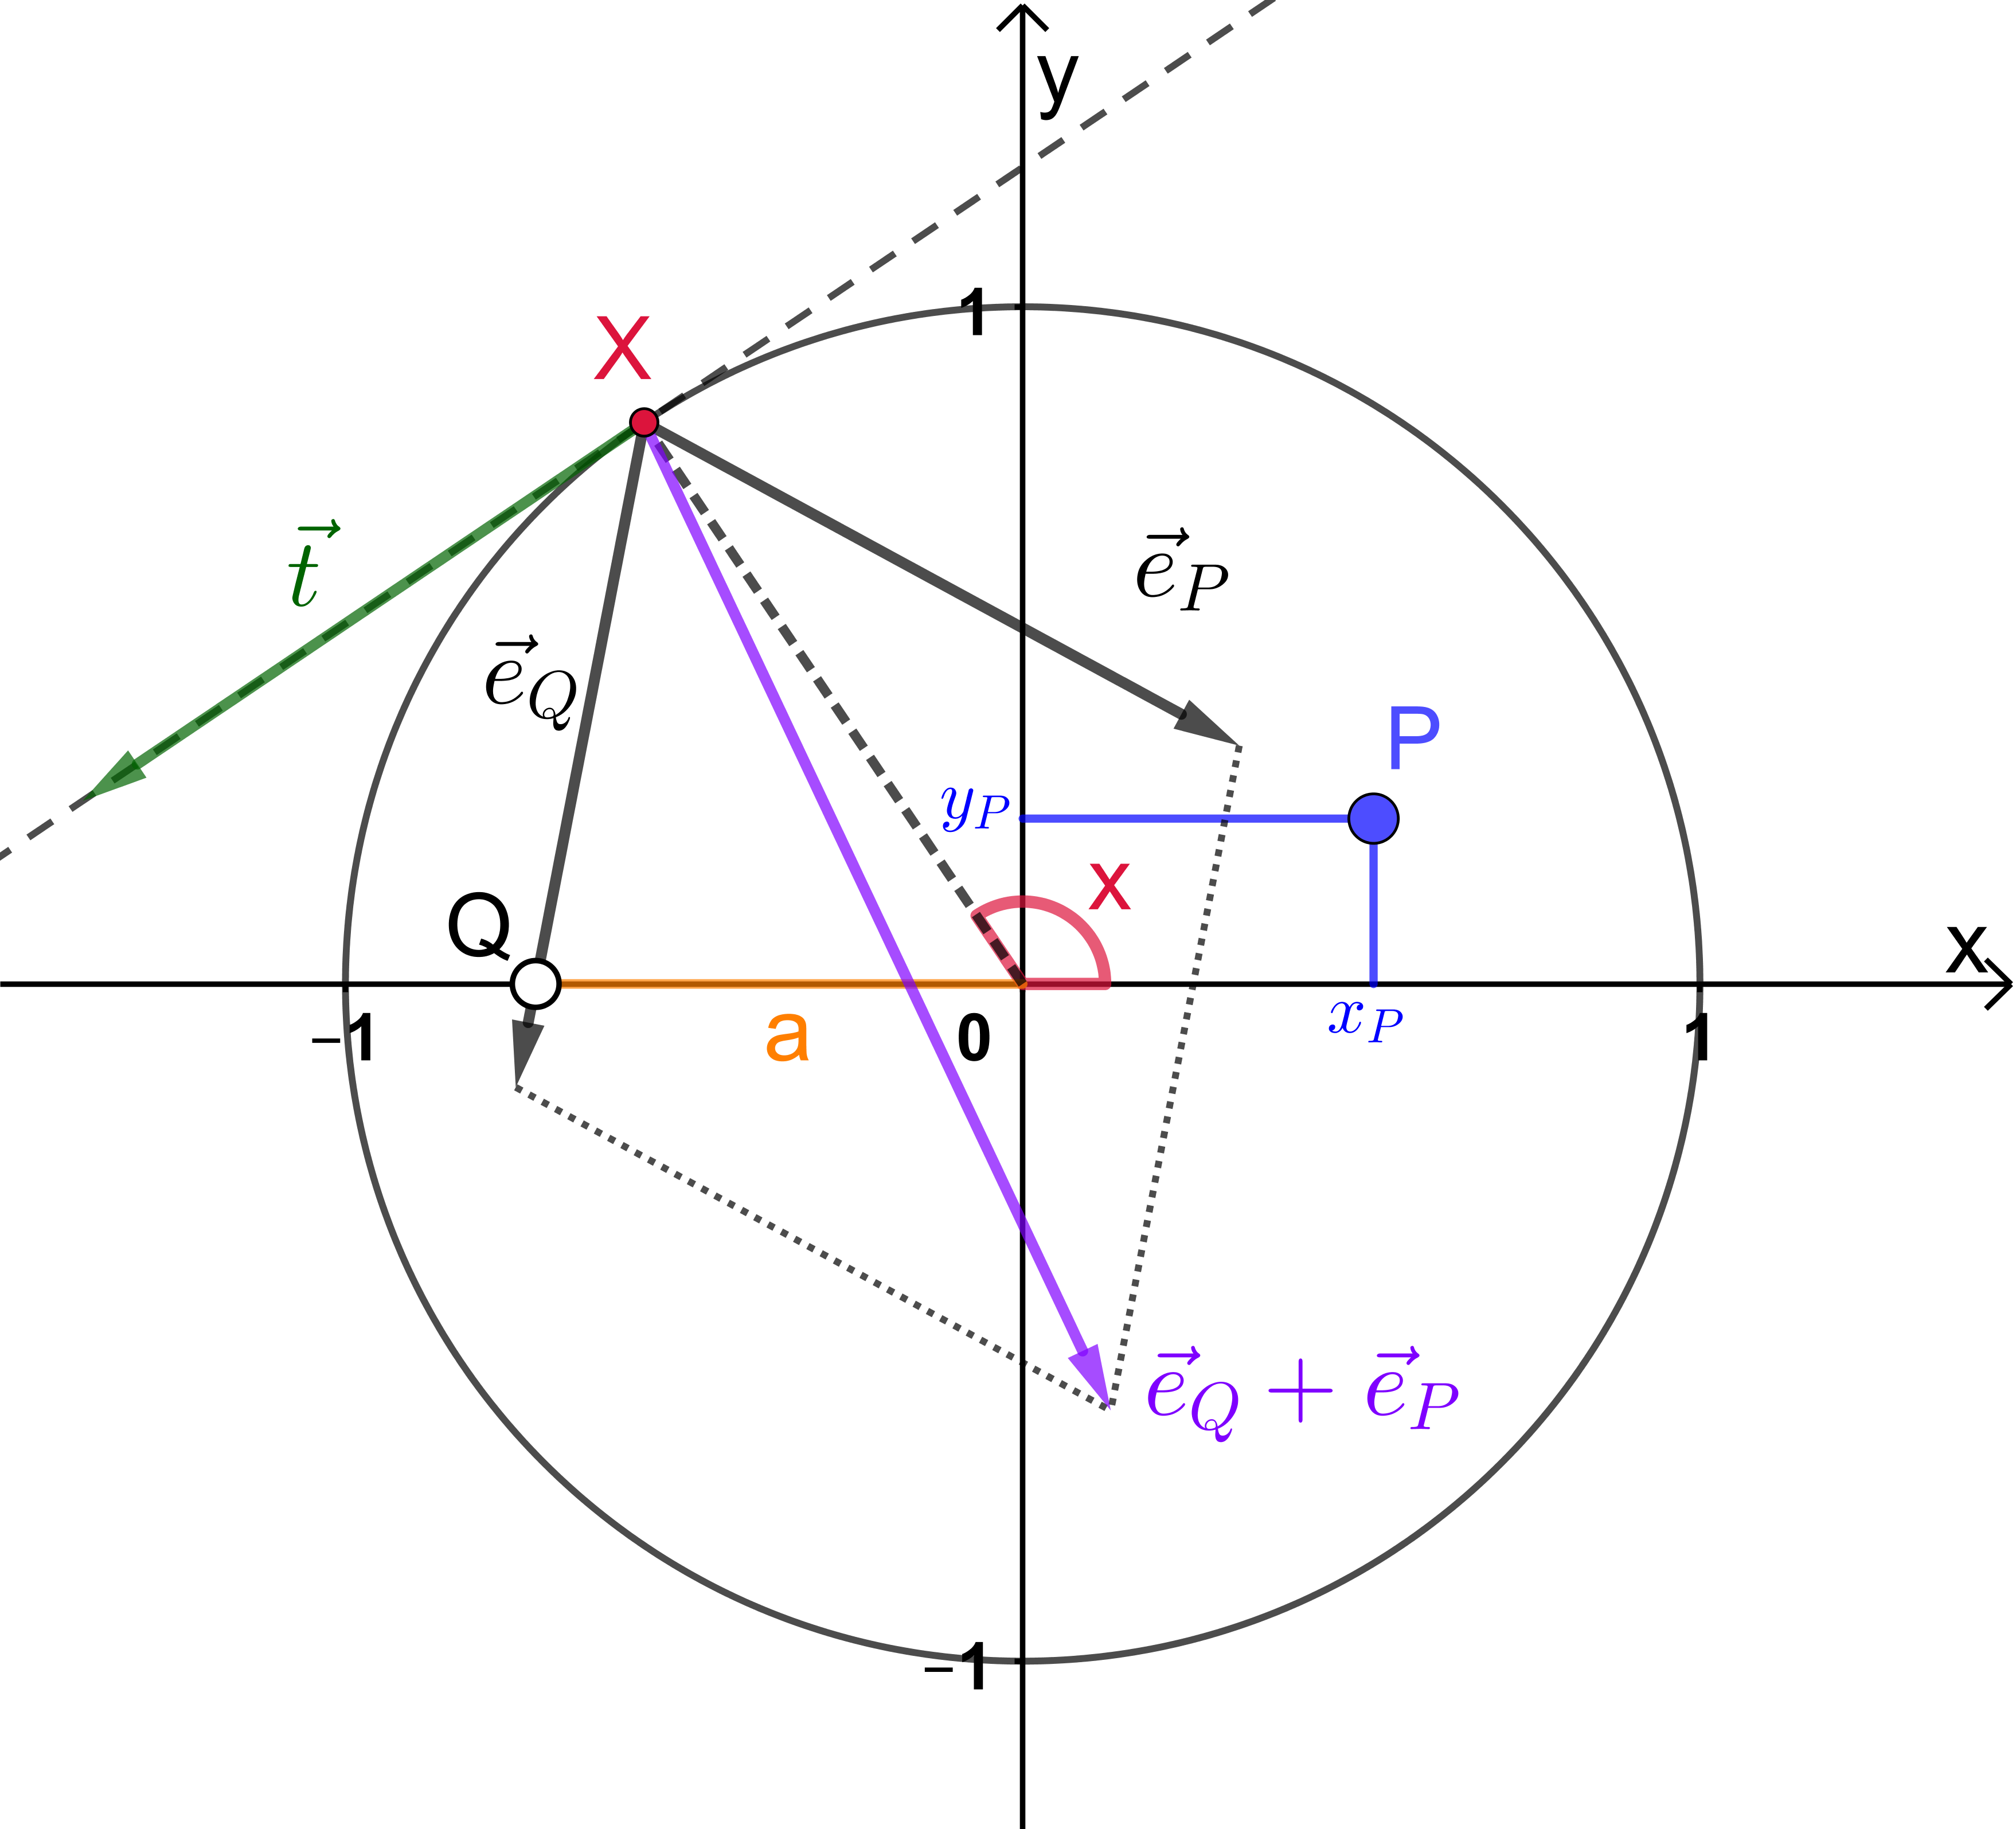
\includegraphics{CircularBillard_sketch.png}

}

\caption{Billard auf einem runden Tisch}

\end{figure}

Wir betrachten nun die Einheitsvektoren \(\vec{e}_Q\) in Richtung
\(\overrightarrow{XQ}\) und \(\vec{e}_P\) in Richtung
\(\overrightarrow{XP}\). Wenn die weisse Kugel die blaue treffen soll,
dann müssen die Winkel zwischen der Tangente und diesen Vektoren gleich
sein. Das ist genau dann der Fall, wenn \(\vec{t}\) senkrecht steht auf
\(\vec{e}_Q + \vec{e}_P\). Wir müssen also \(x\) so bestimmen, dass
\(\vec{t} \cdot (\vec{e}_Q + \vec{e}_P) = 0\) ist.

Das folgende Programm berechnet das Skalarprodukt der linken Seite
dieser Gleichung.

\begin{Shaded}
\begin{Highlighting}[]
\ImportTok{import}\NormalTok{ math}
\ImportTok{import}\NormalTok{ matplotlib.pyplot }\ImportTok{as}\NormalTok{ plt}

\KeywordTok{def}\NormalTok{ f(x):}
    \CommentTok{\# Parameter}
\NormalTok{    a }\OperatorTok{=} \OperatorTok{{-}}\FloatTok{0.8}           \CommentTok{\# Position von Q = (a|0)}
\NormalTok{    px, py }\OperatorTok{=} \FloatTok{0.5}\NormalTok{, }\FloatTok{0.5}  \CommentTok{\# Position von P = (px|py)}

    \CommentTok{\# Berechnung des Skalarprodukts}
\NormalTok{    v0 }\OperatorTok{=}\NormalTok{ x}
\NormalTok{    v1 }\OperatorTok{=}\NormalTok{ math.cos(v0)  }\CommentTok{\# x{-}Koordinate von X}
\NormalTok{    v2 }\OperatorTok{=}\NormalTok{ math.sin(v0)  }\CommentTok{\# y{-}Koordinate von X}
\NormalTok{    v3 }\OperatorTok{=}\NormalTok{ px }\OperatorTok{{-}}\NormalTok{ v1       }\CommentTok{\# x{-}Komponente des Vektors XP}
\NormalTok{    v4 }\OperatorTok{=}\NormalTok{ py }\OperatorTok{{-}}\NormalTok{ v2       }\CommentTok{\# y{-}Komponente des Vektors XP}
\NormalTok{    v5 }\OperatorTok{=}\NormalTok{ math.sqrt(v3}\OperatorTok{**}\DecValTok{2} \OperatorTok{+}\NormalTok{ v4}\OperatorTok{**}\DecValTok{2}\NormalTok{)  }\CommentTok{\# Länge des Vektors XP}
\NormalTok{    v6 }\OperatorTok{=}\NormalTok{ v3 }\OperatorTok{/}\NormalTok{ v5       }\CommentTok{\# x{-}Komponente des Einheitsvektors eP}
\NormalTok{    v7 }\OperatorTok{=}\NormalTok{ v4 }\OperatorTok{/}\NormalTok{ v5       }\CommentTok{\# y{-}Komponente des Einheitsvektors eP}
    
\NormalTok{    v8 }\OperatorTok{=}\NormalTok{ a }\OperatorTok{{-}}\NormalTok{ v1        }\CommentTok{\# x{-}Komponente des Vektors XQ}
\NormalTok{    v9 }\OperatorTok{=} \OperatorTok{{-}}\NormalTok{v2           }\CommentTok{\# y{-}Komponente des Vektors XQ}
\NormalTok{    v10 }\OperatorTok{=}\NormalTok{ math.sqrt(v8}\OperatorTok{**}\DecValTok{2} \OperatorTok{+}\NormalTok{ v9}\OperatorTok{**}\DecValTok{2}\NormalTok{)  }\CommentTok{\# Länge des Vektors XQ}
\NormalTok{    v11 }\OperatorTok{=}\NormalTok{ v8 }\OperatorTok{/}\NormalTok{ v10     }\CommentTok{\# x{-}Komponente des Vektors eQ    }
\NormalTok{    v12 }\OperatorTok{=}\NormalTok{ v9 }\OperatorTok{/}\NormalTok{ v10     }\CommentTok{\# y{-}Komponente des Vektors eQ   }
\NormalTok{    y }\OperatorTok{=}\NormalTok{ (v6 }\OperatorTok{+}\NormalTok{ v11) }\OperatorTok{*}\NormalTok{ v2 }\OperatorTok{{-}}\NormalTok{ (v7 }\OperatorTok{+}\NormalTok{ v12) }\OperatorTok{*}\NormalTok{ v1  }\CommentTok{\# Skalarprodukt}
    \ControlFlowTok{return}\NormalTok{ y   }

\CommentTok{\# Graph der Funktion f(x) plotten}
\NormalTok{fig }\OperatorTok{=}\NormalTok{ plt.figure()}
\NormalTok{ax }\OperatorTok{=}\NormalTok{ plt.gca()}
\NormalTok{ax.set\_xlim((}\DecValTok{0}\NormalTok{,}\DecValTok{2}\OperatorTok{*}\NormalTok{math.pi))}
\NormalTok{ax.set\_ylim((}\OperatorTok{{-}}\FloatTok{1.5}\NormalTok{,}\FloatTok{1.5}\NormalTok{))}
\NormalTok{X }\OperatorTok{=}\NormalTok{ [}\DecValTok{2}\OperatorTok{*}\NormalTok{math.pi }\OperatorTok{*}\NormalTok{ k }\OperatorTok{/} \DecValTok{1000} \ControlFlowTok{for}\NormalTok{ k }\KeywordTok{in} \BuiltInTok{range}\NormalTok{(}\DecValTok{1001}\NormalTok{)]}
\NormalTok{Y }\OperatorTok{=}\NormalTok{ [f(x) }\ControlFlowTok{for}\NormalTok{ x }\KeywordTok{in}\NormalTok{ X]}
\NormalTok{plt.plot([}\DecValTok{0}\NormalTok{, }\DecValTok{2}\OperatorTok{*}\NormalTok{math.pi], [}\DecValTok{0}\NormalTok{, }\DecValTok{0}\NormalTok{], }\StringTok{\textquotesingle{}k{-}{-}\textquotesingle{}}\NormalTok{) }\CommentTok{\# x{-}Achse}
\NormalTok{plt.plot(X,Y)}
\NormalTok{plt.xticks([}\DecValTok{0}\NormalTok{, math.pi}\OperatorTok{/}\DecValTok{2}\NormalTok{, math.pi, }\DecValTok{3}\OperatorTok{*}\NormalTok{math.pi}\OperatorTok{/}\DecValTok{2}\NormalTok{, }\DecValTok{2}\OperatorTok{*}\NormalTok{math.pi],}
\NormalTok{           [}\StringTok{\textquotesingle{}0\textquotesingle{}}\NormalTok{, }\StringTok{\textquotesingle{}π/2\textquotesingle{}}\NormalTok{, }\StringTok{\textquotesingle{}π\textquotesingle{}}\NormalTok{, }\StringTok{\textquotesingle{}3π/2\textquotesingle{}}\NormalTok{, }\StringTok{\textquotesingle{}2π\textquotesingle{}}\NormalTok{])}
\NormalTok{plt.show()  }
\end{Highlighting}
\end{Shaded}

\begin{figure}[H]

{\centering 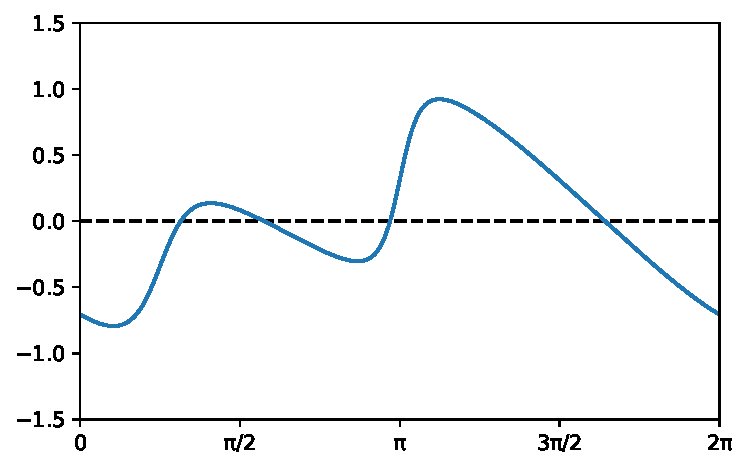
\includegraphics{intro_files/figure-pdf/fig-graphofbillard-output-1.pdf}

}

\caption{\label{fig-graphofbillard}Graph des Skalarprodukts als Funktion
des Polarwinkels \(x\) des Punktes \(X = (cos(x) | sin(x))\). Die
Nullstellen entsprechen den Winkeln, bei denen die weisse Kugel die
blaue Kugel trifft, nachdem sie genau einmal an die Bande gespielt
wurde.}

\end{figure}

Wir möchten die Nullstellen der Funktion \texttt{f(x)} mit unserer
Funtion \texttt{newton} bestimmmen. Dazu müssen wir jedoch die Ableitung
von \texttt{f} berechnen.

\end{example}

\begin{center}\rule{0.5\linewidth}{0.5pt}\end{center}

\hypertarget{sec-gradientDescent}{%
\subsection{Gradient Descent zum Auffinden lokaler
Minima}\label{sec-gradientDescent}}

Eine weitere wichtige Aufgabe besteht darin, ein Minimum einer Funktion
zu finden. Auch hier wollen wir mit Hilfe der Ableitung eine Folge von
Näherungswerten \(x_0, x_1, x_2, \ldots\) finden, deren Grenzwert die
\(x\)-Koordinate eines (lokalen) Minimums von \(f\) ist.

Wenn \(f'(x_n)>0\) ist, dann wissen wir, dass die Funktion \(f\) an der
Stelle \(x_0\) streng monoton wachsend ist. D.h., dass die
Funktionswerte links von \(x_n\) kleiner sind, als an der Stelle
\(x_n\). Analog gilt, dass wenn \(f'(x_n)<0\) ist, die Funktion monoton
fallend ist und wir uns nach rechts bewegen sollten, um ein Minimum zu
finden. In der Nähe eines Minimums ist ausserdem \(|f'(x)|\) sehr klein
und wir können entsprechend kleinere Schritte machen, um uns diesem
anzunähern. Um also von \(x_n\) zu \(x_{n+1}\) zu kommen, machen wir
einen Schritt, der proportional zu \(-f'(x_n)\) ist. Mit dem
Proporionalitätsfaktor \(\lambda\in\mathbb{R}\) und einem geeignet
gewählten Startwert \(x_0\) erhalten wir die Iterationsvorschrift
\begin{equation}\protect\hypertarget{eq-gradientDescent}{}{
x_{n+1} = x_n - \lambda\cdot f'(x_n)
}\label{eq-gradientDescent}\end{equation}

\begin{exercise}[Eigenschaften der Gradient Descent
Methode]\protect\hypertarget{exr-GradientDescentBasicProperties}{}\label{exr-GradientDescentBasicProperties}

Experimentiere mit verschiedenen Funktionen und verschiedenen
Schrittweiten \(\lambda\). Was passiert, wenn die Schrittweite zu klein
bzw. zu gross gewählt wird? Was passiert, wenn \(f\) an der Stelle
\(x_0\) ein lokales Maximum aufweist? Was passiert in der Nähe eines
Sattelpunktes?

\end{exercise}

\begin{tcolorbox}[enhanced jigsaw, titlerule=0mm, title=\textcolor{quarto-callout-tip-color}{\faLightbulb}\hspace{0.5em}{Lösung}, breakable, coltitle=black, leftrule=.75mm, bottomrule=.15mm, colback=white, rightrule=.15mm, opacitybacktitle=0.6, bottomtitle=1mm, toptitle=1mm, left=2mm, toprule=.15mm, colbacktitle=quarto-callout-tip-color!10!white, colframe=quarto-callout-tip-color-frame, arc=.35mm, opacityback=0]

Ist \(\lambda\) zu klein, dann konvergiert das Verfahren nur sehr
langsam. Ist \(\lambda\) dagegen zu gross, dann kann es passieren, dass
die Iteration zwischen zwei oder mehr Werten hin- und herspringt oder
sogar nach \(\pm\infty\) divergiert.

Falls \(x_0\) gerade mit der Stelle eines lokalen Maximums oder eines
Sattelpunktes zusammenfällt, gilt auch \(f'(x_0)=0\) und damit auch
\(x_n = x_0\) für alle \(n\in\mathbb{N}\). Maxima sind aber labile
Gleichgewichtspunkte in dem Sinn, dass sich \(x_n\) von ihnen wegbewegt,
wenn \(x_0\) auch nur ein bisschen links oder rechts davon liegt.
Ähnlich verhält es sich bei Sattelpunkten. Die Folge konvergiert gegen
die Stelle des Sattelpunktes, wenn \(f(x_0)\) grösser als der \(y\)-Wert
des Sattelpunktes ist und \(\lambda\) nicht zu gross ist.

\end{tcolorbox}

\begin{exercise}[Gradient Descent
programmieren]\protect\hypertarget{exr-GradientDescentFirstTry}{}\label{exr-GradientDescentFirstTry}

Schreibe ein Programm, das mit Hilfe des Gradient Descent Verfahrens
(Gleichung~\ref{eq-gradientDescent}) ein lokales Minimums der Funktion
\(f(x) = \frac{1}{16}x^4 - \frac{1}{3}x^3 + \frac{1}{8}x^2 + x + 2\)
berechnet. Verwende den Startwert \(x_0 = 1.5\) und die Schrittweite
\(\lambda = 0.5\). Du kannst abbrechen, wenn die Differenz
\(|x_{n+1} - x_n|\) kleiner als eine bestimmte Toleranz wird, z.B.
kleiner als \texttt{tol\ =\ 1e-6}. Wie flexibel ist dein Programm
einsetzbar? Überlege dir z.B., wie viele Änderungen du vornehmen
müsstest, wenn du ein lokales Minimum einer anderen Funktion berechnen
müsstest.

\end{exercise}

\begin{tcolorbox}[enhanced jigsaw, titlerule=0mm, title=\textcolor{quarto-callout-tip-color}{\faLightbulb}\hspace{0.5em}{Lösung}, breakable, coltitle=black, leftrule=.75mm, bottomrule=.15mm, colback=white, rightrule=.15mm, opacitybacktitle=0.6, bottomtitle=1mm, toptitle=1mm, left=2mm, toprule=.15mm, colbacktitle=quarto-callout-tip-color!10!white, colframe=quarto-callout-tip-color-frame, arc=.35mm, opacityback=0]

Welche der folgenden Lösungsvorschläge kommt deinem Programm am
nächsten?

\section{Version 1}

\begin{Shaded}
\begin{Highlighting}[]
\ImportTok{from}\NormalTok{ math }\ImportTok{import}\NormalTok{ fabs}

\NormalTok{x0 }\OperatorTok{=} \FloatTok{1.5}
\NormalTok{lam }\OperatorTok{=} \FloatTok{0.5}
\NormalTok{tol }\OperatorTok{=} \FloatTok{1e{-}6}
\CommentTok{\# Erster Schritt berechnen}
\NormalTok{x1 }\OperatorTok{=}\NormalTok{ x0 }\OperatorTok{{-}}\NormalTok{ lam }\OperatorTok{*}\NormalTok{ (}\DecValTok{1}\OperatorTok{/}\DecValTok{4} \OperatorTok{*}\NormalTok{ x0}\OperatorTok{**}\DecValTok{3} \OperatorTok{{-}}\NormalTok{ x0}\OperatorTok{**}\DecValTok{2} \OperatorTok{+} \DecValTok{1}\OperatorTok{/}\DecValTok{4} \OperatorTok{*}\NormalTok{ x0 }\OperatorTok{+} \DecValTok{1}\NormalTok{)}
\ControlFlowTok{while}\NormalTok{ fabs(x1}\OperatorTok{{-}}\NormalTok{x0) }\OperatorTok{\textgreater{}}\NormalTok{ tol:}
\NormalTok{    x0 }\OperatorTok{=}\NormalTok{ x1}
\NormalTok{    x1 }\OperatorTok{=}\NormalTok{ x0 }\OperatorTok{{-}}\NormalTok{ lam }\OperatorTok{*}\NormalTok{ (}\DecValTok{1}\OperatorTok{/}\DecValTok{4} \OperatorTok{*}\NormalTok{ x0}\OperatorTok{**}\DecValTok{3} \OperatorTok{{-}}\NormalTok{ x0}\OperatorTok{**}\DecValTok{2} \OperatorTok{+} \DecValTok{1}\OperatorTok{/}\DecValTok{4} \OperatorTok{*}\NormalTok{ x0 }\OperatorTok{+} \DecValTok{1}\NormalTok{)}
\BuiltInTok{print}\NormalTok{(x1)}
\end{Highlighting}
\end{Shaded}

\begin{verbatim}
3.3429230748530196
\end{verbatim}

Das Gradient Descent Verfahren wird als main-Funktion (d.h. im
Hauptprogramm) ausgeführt. Um das Minimum einer anderen Funktion zu
bestimmen, muss ein neues Programm geschrieben werden. Die Ableitung
wurde von Hand berechnet

\section{Version 2}

\begin{Shaded}
\begin{Highlighting}[]
\ImportTok{from}\NormalTok{ math }\ImportTok{import}\NormalTok{ fabs}

\KeywordTok{def}\NormalTok{ fdot(x):}
\NormalTok{    ydot }\OperatorTok{=} \DecValTok{1}\OperatorTok{/}\DecValTok{4} \OperatorTok{*}\NormalTok{ x}\OperatorTok{**}\DecValTok{3} \OperatorTok{{-}}\NormalTok{ x}\OperatorTok{**}\DecValTok{2} \OperatorTok{+} \DecValTok{1}\OperatorTok{/}\DecValTok{4} \OperatorTok{*}\NormalTok{ x }\OperatorTok{+} \DecValTok{1}
    \ControlFlowTok{return}\NormalTok{ ydot}

\NormalTok{x0 }\OperatorTok{=} \FloatTok{1.5}
\NormalTok{lam }\OperatorTok{=} \FloatTok{0.5}
\NormalTok{tol }\OperatorTok{=} \FloatTok{1e{-}6}
\CommentTok{\# Erster Schritt berechnen}
\NormalTok{x1 }\OperatorTok{=}\NormalTok{ x0 }\OperatorTok{{-}}\NormalTok{ lam }\OperatorTok{*}\NormalTok{ fdot(x0)}
\ControlFlowTok{while}\NormalTok{ fabs(x1}\OperatorTok{{-}}\NormalTok{x0) }\OperatorTok{\textgreater{}}\NormalTok{ tol:}
\NormalTok{    x0 }\OperatorTok{=}\NormalTok{ x1}
\NormalTok{    x1 }\OperatorTok{=}\NormalTok{ x0 }\OperatorTok{{-}}\NormalTok{ lam }\OperatorTok{*}\NormalTok{ fdot(x0)}
\BuiltInTok{print}\NormalTok{(x1)}
\end{Highlighting}
\end{Shaded}

\begin{verbatim}
3.3429230748530196
\end{verbatim}

Das Gradient Descent Verfahren wird als main-Funktion (d.h. im
Hauptprogramm) ausgeführt, aber die Berechnung von \(f'\) wurde in die
Funktion \texttt{fdot(x)} ausgelagert. Das macht das Programm etwas
flexibler. Die Ableitung wurde wieder von Hand berechnet.

\section{Version 3}

\begin{Shaded}
\begin{Highlighting}[]
\ImportTok{from}\NormalTok{ math }\ImportTok{import}\NormalTok{ fabs}

\KeywordTok{def}\NormalTok{ gradient\_descent(fdot, x0, lam):}
\NormalTok{    tol }\OperatorTok{=} \FloatTok{1e{-}6}
    \CommentTok{\# Erster Schritt berechnen}
\NormalTok{    x1 }\OperatorTok{=}\NormalTok{ x0 }\OperatorTok{{-}}\NormalTok{ lam }\OperatorTok{*}\NormalTok{ fdot(x0)}
    \ControlFlowTok{while}\NormalTok{ fabs(x1}\OperatorTok{{-}}\NormalTok{x0) }\OperatorTok{\textgreater{}}\NormalTok{ tol:}
\NormalTok{        x0 }\OperatorTok{=}\NormalTok{ x1}
\NormalTok{        x1 }\OperatorTok{=}\NormalTok{ x0 }\OperatorTok{{-}}\NormalTok{ lam }\OperatorTok{*}\NormalTok{ fdot(x0)}
    \ControlFlowTok{return}\NormalTok{ x1}

\KeywordTok{def}\NormalTok{ fdot(x):}
\NormalTok{    ydot }\OperatorTok{=} \DecValTok{1}\OperatorTok{/}\DecValTok{4} \OperatorTok{*}\NormalTok{ x}\OperatorTok{**}\DecValTok{3} \OperatorTok{{-}}\NormalTok{ x}\OperatorTok{**}\DecValTok{2} \OperatorTok{+} \DecValTok{1}\OperatorTok{/}\DecValTok{4} \OperatorTok{*}\NormalTok{ x }\OperatorTok{+} \DecValTok{1}
    \ControlFlowTok{return}\NormalTok{ ydot}

\NormalTok{x0 }\OperatorTok{=} \FloatTok{1.5}
\NormalTok{lam }\OperatorTok{=} \FloatTok{0.5}
\NormalTok{xmin }\OperatorTok{=}\NormalTok{ gradient\_descent(fdot, x0, lam)}
\BuiltInTok{print}\NormalTok{(xmin)}
\end{Highlighting}
\end{Shaded}

\begin{verbatim}
3.3429230748530196
\end{verbatim}

Das Gradient Descent Verfahren wird als eigene Funktion
\texttt{gradient\_descent(fdot,\ x0,\ lam)} implementiert. Dieser
Funktion werden die Ableitung \(f'\), der Startwert \(x_0\), sowie die
Schrittweite \(\lambda\) als Argumente übergeben. Sie kann dann im
Hauptprogramm aufgerufen werden. Die Ableitung wurde aber immer noch von
Hand berechnet.

\section{Version 4}

\begin{Shaded}
\begin{Highlighting}[]
\ImportTok{from}\NormalTok{ math }\ImportTok{import}\NormalTok{ fabs}

\KeywordTok{def}\NormalTok{ gradient\_descent(f, x0, lam):}
\NormalTok{    tol }\OperatorTok{=} \FloatTok{1e{-}6}
    \CommentTok{\# Erster Schritt berechnen}
    \CommentTok{\# Ableitung an der Stelle x0 annähern}
\NormalTok{    h }\OperatorTok{=} \FloatTok{1e{-}6}
\NormalTok{    ydot }\OperatorTok{=}\NormalTok{ ( f(x0 }\OperatorTok{+}\NormalTok{ h) }\OperatorTok{{-}}\NormalTok{ f(x0) ) }\OperatorTok{/}\NormalTok{ h}
\NormalTok{    x1 }\OperatorTok{=}\NormalTok{ x0 }\OperatorTok{{-}}\NormalTok{ lam }\OperatorTok{*}\NormalTok{ ydot}
    \ControlFlowTok{while}\NormalTok{ fabs(x1}\OperatorTok{{-}}\NormalTok{x0) }\OperatorTok{\textgreater{}}\NormalTok{ tol:}
\NormalTok{        x0 }\OperatorTok{=}\NormalTok{ x1}
\NormalTok{        ydot }\OperatorTok{=}\NormalTok{ ( f(x0 }\OperatorTok{+}\NormalTok{ h) }\OperatorTok{{-}}\NormalTok{ f(x0) ) }\OperatorTok{/}\NormalTok{ h}
\NormalTok{        x1 }\OperatorTok{=}\NormalTok{ x0 }\OperatorTok{{-}}\NormalTok{ lam }\OperatorTok{*}\NormalTok{ ydot}
    \ControlFlowTok{return}\NormalTok{ x1}

\KeywordTok{def}\NormalTok{ f(x):}
\NormalTok{    y }\OperatorTok{=} \DecValTok{1}\OperatorTok{/}\DecValTok{16} \OperatorTok{*}\NormalTok{ x}\OperatorTok{**}\DecValTok{4} \OperatorTok{{-}} \DecValTok{1}\OperatorTok{/}\DecValTok{3} \OperatorTok{*}\NormalTok{ x}\OperatorTok{**}\DecValTok{3} \OperatorTok{+} \DecValTok{1}\OperatorTok{/}\DecValTok{8} \OperatorTok{*}\NormalTok{ x}\OperatorTok{**}\DecValTok{2} \OperatorTok{+}\NormalTok{ x }\OperatorTok{+} \DecValTok{2}
    \ControlFlowTok{return}\NormalTok{ y}

\NormalTok{x0 }\OperatorTok{=} \FloatTok{1.5}
\NormalTok{lam }\OperatorTok{=} \FloatTok{0.5}
\NormalTok{xmin }\OperatorTok{=}\NormalTok{ gradient\_descent(fdot, x0, lam)}
\BuiltInTok{print}\NormalTok{(xmin)}
\end{Highlighting}
\end{Shaded}

\begin{verbatim}
2.535183236464121
\end{verbatim}

Das Gradient Descent Verfahren wird als eigene Funktion
\texttt{gradient\_descent(f,\ x0,\ lam)} implementiert. Dieser Funktion
werden die ursprüngliche Funktion \(f\), der Startwert \(x_0\), sowie
die Schrittweite \(\lambda\) als Argumente übergeben. Die Ableitung wird
nicht mehr von Hand berechnet, sondern durch den Differenzenquotienten
\(f'(x_0) \approx \frac{f(x_0 + h) - f(x_0)}{h}\) angenähert. Dabei wird
einfach \texttt{h\ =\ 1e-6} gesetzt und gehofft, dass der entstehende
Rundungsfehler klein genug ist. Offensichtlich ist diese Annahme jedoch
nicht gerechtfertigt.

\end{tcolorbox}

Die Übungsaufgabe~\ref{exr-GradientDescentFirstTry} verdeutlicht
nochmals das Problem, welches wir bereits in
Übungsaufgabe~\ref{exr-NewtonFirstTry} gesehen haben. Wir müssen für den
Algorithmus die Ableitung \(f'\) an mehreren Stellen auswerten. Wir
möchten aber die Ableitung einerseits nicht von Hand berechnen und
andererseits können wir uns auch nicht mit einer Approximation zufrieden
geben.

Wir beschliessen dieses Kapitel mit einer praktischen Anwendung der
Gradient Descent Methode.

\begin{example}[Minimaler
Abstand]\protect\hypertarget{exm-GDApplication}{}\label{exm-GDApplication}

Die Punkte \(P\) und \(Q\) bewegen sich auf Ellipsen im Raum. Die
Position des Punktes \(P\) zur Zeit \(t\) ist gegeben durch

\begin{align*}
    x_P(t) &= 2 \cos(t) - 1 \\
    y_P(t) &= 1.5 \sin(t)   \\
    z_P(t) &= 0             
\end{align*}

und die Position von \(Q\) zum Zeitpunkt \(t\) lässt sich durch

\begin{align*}
    x_Q(t) &= -3 \sin(2t)     \\
    y_Q(t) &= 2 \cos(2t) + 1  \\
    z_Q(t) &= 2 \sin(2t) + 1  
\end{align*}

bestimmen.

Der Abstand zwischen den beiden Punkten lässt sich zu jedem Zeitpunkt
\(t\) berechnen durch \(d = d(t) = |\overrightarrow{PQ}|\). Das folgende
Programm berechnet diese Funktion und zeichnet ihren Graph.

\begin{Shaded}
\begin{Highlighting}[]
\ImportTok{import}\NormalTok{ math}
\ImportTok{import}\NormalTok{ matplotlib.pyplot }\ImportTok{as}\NormalTok{ plt}

\KeywordTok{def}\NormalTok{ d(t):}
\NormalTok{    v0 }\OperatorTok{=}\NormalTok{ t}
\NormalTok{    v1 }\OperatorTok{=} \DecValTok{2} \OperatorTok{*}\NormalTok{ math.cos(v0) }\OperatorTok{{-}} \DecValTok{1}    \CommentTok{\# x{-}Koordinate von P}
\NormalTok{    v2 }\OperatorTok{=} \FloatTok{1.5} \OperatorTok{*}\NormalTok{ math.sin(v0)      }\CommentTok{\# y{-}Koordinate von P}
\NormalTok{    v3 }\OperatorTok{=} \DecValTok{0}                       \CommentTok{\# z{-}Koordinate von P}
\NormalTok{    v4 }\OperatorTok{=} \OperatorTok{{-}}\DecValTok{3} \OperatorTok{*}\NormalTok{ math.sin(}\DecValTok{2}\OperatorTok{*}\NormalTok{v0)     }\CommentTok{\# x{-}Koordinate von Q}
\NormalTok{    v5 }\OperatorTok{=} \DecValTok{2} \OperatorTok{*}\NormalTok{ math.cos(}\DecValTok{2}\OperatorTok{*}\NormalTok{v0) }\OperatorTok{+} \DecValTok{1}  \CommentTok{\# y{-}Koordinate von Q}
\NormalTok{    v6 }\OperatorTok{=} \DecValTok{2} \OperatorTok{*}\NormalTok{ math.sin(}\DecValTok{2}\OperatorTok{*}\NormalTok{v0) }\OperatorTok{+} \DecValTok{1}  \CommentTok{\# z{-}Koordinate von Q}
\NormalTok{    y }\OperatorTok{=}\NormalTok{ math.sqrt((v4}\OperatorTok{{-}}\NormalTok{v1)}\OperatorTok{**}\DecValTok{2} \OperatorTok{+}\NormalTok{ (v5}\OperatorTok{{-}}\NormalTok{v2)}\OperatorTok{**}\DecValTok{2} \OperatorTok{+}\NormalTok{ (v6}\OperatorTok{{-}}\NormalTok{v3)}\OperatorTok{**}\DecValTok{2}\NormalTok{)}
    \ControlFlowTok{return}\NormalTok{ y}

\CommentTok{\# Graph der Funktion d(t) plotten}
\NormalTok{fig }\OperatorTok{=}\NormalTok{ plt.figure()}
\NormalTok{ax }\OperatorTok{=}\NormalTok{ plt.gca()}
\NormalTok{ax.set\_xlim((}\DecValTok{0}\NormalTok{,}\DecValTok{2}\OperatorTok{*}\NormalTok{math.pi))}
\NormalTok{ax.set\_ylim((}\DecValTok{0}\NormalTok{,}\DecValTok{6}\NormalTok{))}
\NormalTok{T }\OperatorTok{=}\NormalTok{ [}\DecValTok{2}\OperatorTok{*}\NormalTok{math.pi }\OperatorTok{*}\NormalTok{ k }\OperatorTok{/} \DecValTok{1000} \ControlFlowTok{for}\NormalTok{ k }\KeywordTok{in} \BuiltInTok{range}\NormalTok{(}\DecValTok{1001}\NormalTok{)]}
\NormalTok{Y }\OperatorTok{=}\NormalTok{ [d(t) }\ControlFlowTok{for}\NormalTok{ t }\KeywordTok{in}\NormalTok{ T]}
\NormalTok{plt.plot(T,Y)}
\NormalTok{plt.xticks([}\DecValTok{0}\NormalTok{, math.pi}\OperatorTok{/}\DecValTok{2}\NormalTok{, math.pi, }\DecValTok{3}\OperatorTok{*}\NormalTok{math.pi}\OperatorTok{/}\DecValTok{2}\NormalTok{, }\DecValTok{2}\OperatorTok{*}\NormalTok{math.pi],}
\NormalTok{           [}\StringTok{\textquotesingle{}0\textquotesingle{}}\NormalTok{, }\StringTok{\textquotesingle{}π/2\textquotesingle{}}\NormalTok{, }\StringTok{\textquotesingle{}π\textquotesingle{}}\NormalTok{, }\StringTok{\textquotesingle{}3π/2\textquotesingle{}}\NormalTok{, }\StringTok{\textquotesingle{}2π\textquotesingle{}}\NormalTok{])}
\NormalTok{plt.show()  }
\end{Highlighting}
\end{Shaded}

\begin{figure}[H]

{\centering 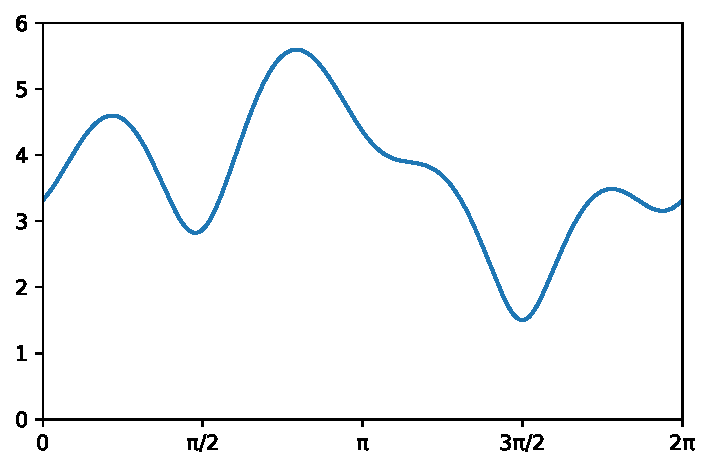
\includegraphics{intro_files/figure-pdf/fig-graphofdistanceproblem-output-1.pdf}

}

\caption{\label{fig-graphofdistanceproblem}Graph der Abstandsfunktion
\(d(t)\).}

\end{figure}

Wir möchten das Minimum der Funktion \(d(t)\) mit Hilfe der Gradient
Descent Methode finden. Dazu müssen wir aber \(d\) ableiten können.

\end{example}

\begin{center}\rule{0.5\linewidth}{0.5pt}\end{center}

\bookmarksetup{startatroot}

\hypertarget{sec-ADisnot}{%
\chapter{AD ist nicht \ldots{}}\label{sec-ADisnot}}

Bevor wir uns mit den konkreten Implementationen von algorithmischer
Differentiation beschäftigen, wollen wir herausstellen, was AD
\emph{nicht} ist.

\hypertarget{sec-ADnotNumDiff}{%
\section{AD ist nicht numerisches Ableiten}\label{sec-ADnotNumDiff}}

Eine Funktion \(y = f(x)\) ist bekanntlich differenzierbar an der Stelle
\(x_0 \in \mathbb{D}\), wenn der Grenzwert
\[ \lim_{h\rightarrow 0} \frac{f(x_0 + h) - f(x_0)}{h} \] existiert. In
dem Fall ist \(f'(x_0)\) einfach der Wert dieses Grenzwerts.

Ein erster Ansatz zur numerischen Berechnung könnte also sein, den
Differenzenquotienten für kleine \(h\) auszuwerten\footnote{Dieser
  Ansatz kann verbessert werden indem man z.B.
  \(f'(x_0) \approx \frac{f(x_0 + h) - f(x_0 - h)}{2h}\) verwendet. Die
  im Beispiel beschriebenen Probleme bleiben aber auch dann bestehen.}.

\begin{example}[Numerische
Ableitung]\protect\hypertarget{exm-numDiff}{}\label{exm-numDiff}

Leite die Funktion \(f(x) = x^2\) an der Stelle \(x_0 = 0.2\) ab.

\begin{Shaded}
\begin{Highlighting}[]
\KeywordTok{def}\NormalTok{ f(x):}
\NormalTok{    y }\OperatorTok{=}\NormalTok{ x }\OperatorTok{**} \DecValTok{2}
    \ControlFlowTok{return}\NormalTok{ y}

\KeywordTok{def}\NormalTok{ fdot(f, x0, h):}
\NormalTok{    df }\OperatorTok{=}\NormalTok{ (f(x0 }\OperatorTok{+}\NormalTok{ h) }\OperatorTok{{-}}\NormalTok{ f(x0)) }\OperatorTok{/}\NormalTok{ h}
    \ControlFlowTok{return}\NormalTok{ df}

\NormalTok{x0 }\OperatorTok{=} \FloatTok{0.2}
\NormalTok{H }\OperatorTok{=}\NormalTok{ [}\FloatTok{0.1}\NormalTok{, }\FloatTok{0.01}\NormalTok{, }\FloatTok{0.001}\NormalTok{, }\FloatTok{0.0001}\NormalTok{]}
\ControlFlowTok{for}\NormalTok{ h }\KeywordTok{in}\NormalTok{ H:}
\NormalTok{    ydot }\OperatorTok{=}\NormalTok{ fdot(f, x0, h)}
    \BuiltInTok{print}\NormalTok{(}\StringTok{"h = "} \OperatorTok{+} \BuiltInTok{str}\NormalTok{(h) }\OperatorTok{+} \StringTok{" }\CharTok{\textbackslash{}t}\StringTok{=\textgreater{} f\textquotesingle{}(x0) = "} \OperatorTok{+} \BuiltInTok{str}\NormalTok{(ydot))}
\end{Highlighting}
\end{Shaded}

\begin{verbatim}
h = 0.1     => f'(x0) = 0.5000000000000001
h = 0.01    => f'(x0) = 0.4099999999999999
h = 0.001   => f'(x0) = 0.4009999999999986
h = 0.0001  => f'(x0) = 0.40009999999993107
\end{verbatim}

Es scheint zunächst, als ob die Werte für kleiner werdende \(h\) zum
korrekten Wert \(f'(0.2)=0.4\) konvergieren. Wenn wir aber an sehr
genauen Werten interessiert sind und entsprechend \(h\) sehr klein
wählen, beobachten wir folgendes:

\begin{Shaded}
\begin{Highlighting}[]
\KeywordTok{def}\NormalTok{ f(x):}
\NormalTok{    y }\OperatorTok{=}\NormalTok{ x }\OperatorTok{**} \DecValTok{2}
    \ControlFlowTok{return}\NormalTok{ y}

\KeywordTok{def}\NormalTok{ fdot(f, x0, h):}
\NormalTok{    df }\OperatorTok{=}\NormalTok{ (f(x0 }\OperatorTok{+}\NormalTok{ h) }\OperatorTok{{-}}\NormalTok{ f(x0)) }\OperatorTok{/}\NormalTok{ h}
    \ControlFlowTok{return}\NormalTok{ df}

\NormalTok{x0 }\OperatorTok{=} \FloatTok{0.2}
\NormalTok{H }\OperatorTok{=}\NormalTok{ [}\DecValTok{10} \OperatorTok{**} \OperatorTok{{-}}\DecValTok{8}\NormalTok{, }\DecValTok{10} \OperatorTok{**} \OperatorTok{{-}}\DecValTok{9}\NormalTok{, }\DecValTok{10} \OperatorTok{**} \OperatorTok{{-}}\DecValTok{10}\NormalTok{, }\DecValTok{10} \OperatorTok{**} \OperatorTok{{-}}\DecValTok{11}\NormalTok{]}
\ControlFlowTok{for}\NormalTok{ h }\KeywordTok{in}\NormalTok{ H:}
\NormalTok{    ydot }\OperatorTok{=}\NormalTok{ fdot(f, x0, h)}
    \BuiltInTok{print}\NormalTok{(}\StringTok{"h = "} \OperatorTok{+} \BuiltInTok{str}\NormalTok{(h) }\OperatorTok{+} \StringTok{"}\CharTok{\textbackslash{}t}\StringTok{=\textgreater{} f\textquotesingle{}(x0) = "} \OperatorTok{+} \BuiltInTok{str}\NormalTok{(ydot))}
\end{Highlighting}
\end{Shaded}

\begin{verbatim}
h = 1e-08   => f'(x0) = 0.4000000095039091
h = 1e-09   => f'(x0) = 0.3999999984016789
h = 1e-10   => f'(x0) = 0.4000000330961484
h = 1e-11   => f'(x0) = 0.3999994779846361
\end{verbatim}

Mit kleiner werdendem \(h\) scheint sich der Näherungswert für die
Ableitung zu verschlechtern. Das Phänomen wird noch deutlicher, wenn wir
den Fehler \(E(h) = \lvert\frac{f(x_0+h)-f(x_0)}{h} - f'(x_0)\rvert\)
als Funktion von \(h\) plotten. Beachte die doppelt logarithmische
Skala.

\begin{Shaded}
\begin{Highlighting}[]
\ImportTok{import}\NormalTok{ matplotlib.pyplot }\ImportTok{as}\NormalTok{ plt}
\ImportTok{import}\NormalTok{ math}

\KeywordTok{def}\NormalTok{ f(x):}
\NormalTok{    y }\OperatorTok{=}\NormalTok{ x }\OperatorTok{**} \DecValTok{2}
    \ControlFlowTok{return}\NormalTok{ y}

\KeywordTok{def}\NormalTok{ fdot(f, x0, h):}
\NormalTok{    df }\OperatorTok{=}\NormalTok{ (f(x0 }\OperatorTok{+}\NormalTok{ h) }\OperatorTok{{-}}\NormalTok{ f(x0)) }\OperatorTok{/}\NormalTok{ h}
    \ControlFlowTok{return}\NormalTok{ df}

\NormalTok{x0 }\OperatorTok{=} \FloatTok{0.2}
\NormalTok{H }\OperatorTok{=}\NormalTok{ [}\DecValTok{10}\OperatorTok{**}\NormalTok{(k}\OperatorTok{/}\DecValTok{100}\NormalTok{) }\ControlFlowTok{for}\NormalTok{ k }\KeywordTok{in} \BuiltInTok{range}\NormalTok{(}\OperatorTok{{-}}\DecValTok{1800}\NormalTok{, }\OperatorTok{{-}}\DecValTok{300}\NormalTok{)]}
\NormalTok{E }\OperatorTok{=}\NormalTok{ [math.fabs(fdot(f, x0, h) }\OperatorTok{{-}} \DecValTok{2}\OperatorTok{*}\NormalTok{x0) }\ControlFlowTok{for}\NormalTok{ h }\KeywordTok{in}\NormalTok{ H]}

\CommentTok{\# Plot}
\NormalTok{fig }\OperatorTok{=}\NormalTok{ plt.figure()}
\NormalTok{ax }\OperatorTok{=}\NormalTok{ fig.add\_axes([}\FloatTok{0.1}\NormalTok{, }\FloatTok{0.1}\NormalTok{, }\FloatTok{0.8}\NormalTok{, }\FloatTok{0.8}\NormalTok{])}
\NormalTok{ax.}\BuiltInTok{set}\NormalTok{(xlim}\OperatorTok{=}\NormalTok{(}\DecValTok{10}\OperatorTok{**{-}}\DecValTok{18}\NormalTok{, }\DecValTok{10}\OperatorTok{**{-}}\DecValTok{3}\NormalTok{), ylim}\OperatorTok{=}\NormalTok{(}\DecValTok{10}\OperatorTok{**{-}}\DecValTok{12}\NormalTok{, }\DecValTok{10}\OperatorTok{**}\DecValTok{0}\NormalTok{))}
\NormalTok{ax.set\_xscale(}\StringTok{\textquotesingle{}log\textquotesingle{}}\NormalTok{)}
\NormalTok{ax.set\_xlabel(}\StringTok{\textquotesingle{}h\textquotesingle{}}\NormalTok{)}
\NormalTok{ax.set\_yscale(}\StringTok{\textquotesingle{}log\textquotesingle{}}\NormalTok{)}
\NormalTok{ax.set\_ylabel(}\StringTok{\textquotesingle{}Fehler E(h)\textquotesingle{}}\NormalTok{)}
\NormalTok{plt.plot(H,E)}
\NormalTok{plt.show()}
\end{Highlighting}
\end{Shaded}

\begin{figure}[H]

{\centering 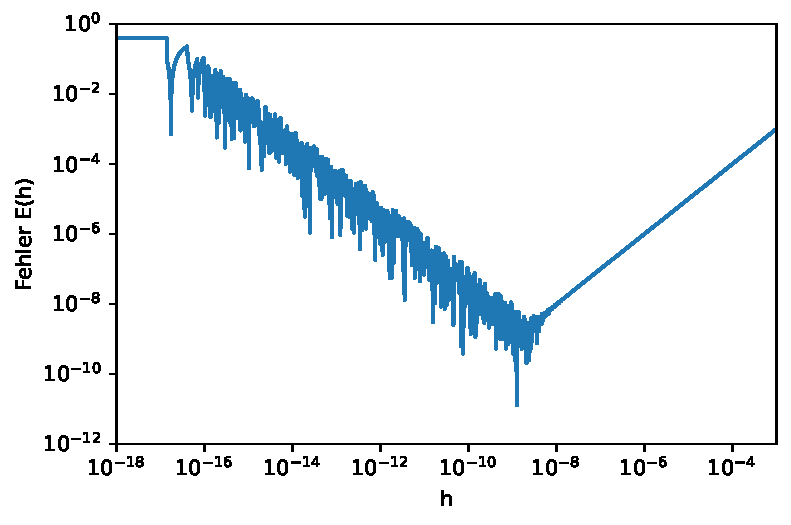
\includegraphics{notAD_files/figure-pdf/fig-numdiffproblem-output-1.pdf}

}

\caption{\label{fig-numdiffproblem}Grösse des Fehlers \(E(h)\) als
Funktion der Schrittweite \(h\). Ist \(h\) zu gross, dann ist der
Näherungswert für \(f'(x_0)\) ungenau. Bei kleiner werdendem \(h\) nimmt
der Fehler zunächst ab, aber ab einem gewissen Wert dominiert die
Auslöschung und der Fehler nimmt wieder zu.}

\end{figure}

\end{example}

\begin{center}\rule{0.5\linewidth}{0.5pt}\end{center}

\hypertarget{ausluxf6schung}{%
\subsection{Auslöschung}\label{ausluxf6schung}}

Im vorherigen Beispiel haben wir das Phänomen der
\href{https://de.wikipedia.org/wiki/Ausl\%C3\%B6schung_(numerische_Mathematik)}{Auslöschung}
beobachtet. Zunächst ist dir sicher aufgefallen, dass der Näherungswert
für \(f'(x_0)\) mit \(h=0.01\) nicht
\[ \frac{f(x_0 + h) - f(x_0)}{h} = \frac{0.21^2 - 0.2^2}{0.01}=0.41\]
ergab, sondern \(f'(x_0)\approx 0.40999...\). Das liegt daran, dass
Dezimalzahlen nicht exakt als Binärzahl dargestellt werden können. Da
nun die Werte von \(f(x_0 + h)\) und \(f(x_0)\) für kleine \(h\) fast
gleich sind, besteht ihre Differenz \(f(x_0 + h) - f(x_0)\) nur noch aus
diesen Rundungsfehlern. Diese (sinnlose) Differenz ist zwar sehr klein,
wird aber im nächsten Schritt mit der sehr grossen Zahl \(\frac{1}{h}\)
multipliziert, wodurch die Rundungsfehler die gleiche Grössenordnung
annehmen, wie die ursprünglichen Funktionswerte. Mehr über
Rundungsfehler und Auslöschung kann in Weitz (2021) ab S. 117
nachgelesen werden.

\hypertarget{sec-ADnotSymbDiff}{%
\section{AD ist nicht symbolisches Ableiten}\label{sec-ADnotSymbDiff}}

Computer Algebra Systeme (CAS) sind Programme zur Bearbeitung
algebraischer Ausdrücke. Mit solchen Programmen lassen sich auch
Ableitungen symbolisch bestimmen. Wie das funktioniert, wird in Slater
(2022) kurz angedeutet. Bekannte Beispiele für CAS sind etwa
\href{https://www.wolframalpha.com/}{Wolfram Alpha},
\href{https://maxima.sourceforge.io/download.html}{Maxima} oder
\href{https://www.sagemath.org/}{Sage}. Letzteres kann man
\href{https://sagecell.sagemath.org/}{hier} auch online ausprobieren.
Gib z.B. den folgenden Code ein, welcher die Ableitung der Funktion aus
Übungsaufgabe~\ref{exr-LoopProgToFun} bestimmt:

\begin{verbatim}
l(x) = x^2 + 1
f(x) = l(l(l(x)))
fdot = diff(f,x)
expand(fdot)
\end{verbatim}

\begin{tcolorbox}[enhanced jigsaw, titlerule=0mm, title=\textcolor{quarto-callout-tip-color}{\faLightbulb}\hspace{0.5em}{Tipp}, breakable, coltitle=black, leftrule=.75mm, bottomrule=.15mm, colback=white, rightrule=.15mm, opacitybacktitle=0.6, bottomtitle=1mm, toptitle=1mm, left=2mm, toprule=.15mm, colbacktitle=quarto-callout-tip-color!10!white, colframe=quarto-callout-tip-color-frame, arc=.35mm, opacityback=0]

Auf der Website kannst du rechts unter \texttt{Language} auch
\texttt{Maxima} auswählen und Maxima-Code ausführen. Maxima ist in Sage
integriert.

\end{tcolorbox}

Für Python gibt es die Bibliothek \texttt{sympy}, die ein CAS für Python
zur Verfügung stellt. Damit können wir die Funktion aus
Übungsaufgabe~\ref{exr-LoopProgToFun} direkt in Python ableiten:

\begin{example}[Symbolische
Ableitung]\protect\hypertarget{exm-symbDiff}{}\label{exm-symbDiff}

Leite die Funktion \(f(x) = l(l(l(x)))\), wobei \(l(x) = x^2 + 1\) ist,
an der Stelle \(x_0 = 1\) ab.

\begin{Shaded}
\begin{Highlighting}[]
\ImportTok{from}\NormalTok{ sympy }\ImportTok{import}\NormalTok{ symbols, diff}

\KeywordTok{def}\NormalTok{ f(x):}
\NormalTok{    v0 }\OperatorTok{=}\NormalTok{ x}
\NormalTok{    v1 }\OperatorTok{=}\NormalTok{ v0 }\OperatorTok{**} \DecValTok{2} \OperatorTok{+} \DecValTok{1}
\NormalTok{    v2 }\OperatorTok{=}\NormalTok{ v1 }\OperatorTok{**} \DecValTok{2} \OperatorTok{+} \DecValTok{1}
\NormalTok{    v3 }\OperatorTok{=}\NormalTok{ v2 }\OperatorTok{**} \DecValTok{2} \OperatorTok{+} \DecValTok{1}
\NormalTok{    y }\OperatorTok{=}\NormalTok{ v3}
    \ControlFlowTok{return}\NormalTok{ y}

\NormalTok{x }\OperatorTok{=}\NormalTok{ symbols(}\StringTok{\textquotesingle{}x\textquotesingle{}}\NormalTok{)}
\BuiltInTok{print}\NormalTok{(}\StringTok{"f(x) ="}\NormalTok{, f(x))}

\NormalTok{df }\OperatorTok{=}\NormalTok{ diff(f(x),x)}
\BuiltInTok{print}\NormalTok{(}\StringTok{"f\textquotesingle{}(x) ="}\NormalTok{, df)}

\NormalTok{x0 }\OperatorTok{=} \DecValTok{1}
\BuiltInTok{print}\NormalTok{(}\StringTok{"f\textquotesingle{}("} \OperatorTok{+} \BuiltInTok{str}\NormalTok{(x0) }\OperatorTok{+} \StringTok{") ="}\NormalTok{, df.evalf(subs}\OperatorTok{=}\NormalTok{\{x:x0\}))}
\end{Highlighting}
\end{Shaded}

\begin{verbatim}
f(x) = ((x**2 + 1)**2 + 1)**2 + 1
f'(x) = 8*x*(x**2 + 1)*((x**2 + 1)**2 + 1)
f'(1) = 80.0000000000000
\end{verbatim}

\end{example}

\begin{center}\rule{0.5\linewidth}{0.5pt}\end{center}

Damit erhält man die (bis auf Maschinengenauigkeit) exakten Werte der
Ableitungen. Der Grund, warum wir nicht auf symbolische Ausdrücke für
Ableitungen zurückgreifen wollen, liegt darin, dass diese Methode bei
komplizierten Funktionsausdrücken sehr ineffizient ist, insbesondere
dann, wenn wir auch Ableitungen von Funktionen
\(f : \mathbb{R}^n \rightarrow \mathbb{R}^m\) berechnen wollen.

\bookmarksetup{startatroot}

\hypertarget{sec-SADforOneDimFunctions}{%
\chapter{Standard Algorithmische Differentiation für eindimensionale
Funktionen}\label{sec-SADforOneDimFunctions}}

In Kapitel~\ref{sec-ADisnot} haben wir zwei Methoden für die Berechnung
von Ableitungen kennen gelernt, die beide ihre Schwächen haben. Während
die numerische Ableitung mit geringem Aufwand berechnet werden kann,
sind ihre Näherungswerte für viele Anwendungen zu ungenau. Symbolische
Ableitungen andererseits liefern zwar exakte Werte von Ableitungen, sind
aber mit grossem Rechenaufwand verbunden. Die hier vorgestellte
Algorithmische Differentiation (AD) vereinigt die Vorteile der beiden
Methoden. Sie liefert uns (bis auf Maschinengenauigkeit) exakte Werte
von Ableitungen mit nur einem geringen zusätzlichen Rechenaufwand:

\begin{quote}
``AD as a technical term refers to a specific family of techniques that
compute derivatives trhough accumulation of values during code execution
to generate numerical derivative evaluations rather than derivative
expressions. This allows accurate evaluation of derivatives at machine
precision with only a small constant factor of overhead and ideal
asymptotic efficiency.'' (Baydin u.~a. (2018), S. 2)
\end{quote}

In diesem Kapitel lernen wir die \emph{Standard Algorithmische
Differentiation} (SAD, auch Vorwärts-AD genannt) kennen, welche die
einfachste Variante der erwähnten ``family of techniques'' ist. Wir
beschränken uns zunächst wieder auf Funktionen
\(f : \mathbb{R} \rightarrow \mathbb{R}\) und werden dies später auf
Funktionen \(f : \mathbb{R}^n \rightarrow \mathbb{R}^m\) erweitern.
Neben der Standard-AD gibt es noch die \emph{Adjungierte Algorithmische
Differentiation} (AAD, auch Rückwärts-AD genannt). Die Vorteile dieser
Methode offenbaren sich jedoch erst für Funktionen in höherdimensionalen
Räumen. Der interessierte Leser findet hierzu eine kurze Einführung in
Kapitel~\ref{sec-AAD}.

Gemäss unserer Konvention in Kapitel~\ref{sec-ProgFunc} berechnen wir
eine mathematische Funktion, indem wir sie in ihre Bestandteile
zerlegen, und die Zwischenergebnisse Variablen \texttt{v} zuweisen. Wie
im obigen Zitat erwähnt, besteht die Grundidee der AD darin, eine Reihe
von Hilfsvariablen \texttt{vdot} einzuführen, welche jeweils die Werte
der Ableitungen enthalten. In diesem Kapitel machen wir dies explizit,
indem wir jede Programmzeile, die ein \texttt{v} berechnet, um die
Berechnung des zugehörigen \texttt{vdot} erweitern. Dies scheint
zunächst umständlich zu sein, aber im nächsten Abschnitt werden wir eine
Klasse schreiben, die diese Schritte für uns automatisiert. Wie Marc
Henrard in seinem Buch schreibt:

\begin{quote}
``There are as many shades of AD as there are AD users. {[}This
chapter{]} provides to the user the black and the white; it is up to him
to get the correct shade of grey that fits his taste and his
requirements.'' (Henrard (2017), S. 18)
\end{quote}

\hypertarget{sec-SadManualImplementation}{%
\section{Manuelle Implementation der
SAD}\label{sec-SadManualImplementation}}

Beginnen wir mit einem Beispiel:

Wir möchten den Funktionswert und die Ableitung der Funktion
\(y=f(x)=\sin(x^2)\) an der Stelle \(x_0=\frac{\pi}{2}\) bestimmen. Das
folgende Programm berechnet den Funktionswert.

\begin{Shaded}
\begin{Highlighting}[]
\ImportTok{import}\NormalTok{ math}

\KeywordTok{def}\NormalTok{ f(x):}
\NormalTok{    v0 }\OperatorTok{=}\NormalTok{ x}
\NormalTok{    v1 }\OperatorTok{=}\NormalTok{ v0}\OperatorTok{**}\DecValTok{2}
\NormalTok{    v2 }\OperatorTok{=}\NormalTok{ math.sin(v1)}
\NormalTok{    y }\OperatorTok{=}\NormalTok{ v2}
    \ControlFlowTok{return}\NormalTok{ y}

\NormalTok{x0 }\OperatorTok{=}\NormalTok{ math.pi }\OperatorTok{/} \DecValTok{2}
\BuiltInTok{print}\NormalTok{(f(x0))}
\end{Highlighting}
\end{Shaded}

\begin{verbatim}
0.6242659526396992
\end{verbatim}

\(f\) ist eine zusammengesetzte Funktion, die wir mit den Funktionen

\begin{align*}
    v_0(x)   &= x \\
    v_1(v_0) &= v_0 ^2 \\
    v_2(v_1) &= \sin(v_1)
\end{align*}

schreiben können als \(y=f(x)=v_2(v_1(v_0(x)))\). Die Ableitung
berechnet sich dann mit der Kettenregel zu \[
f'(x) = \frac{dv_2}{dv_1} \cdot \frac{dv_1}{dv_0} \cdot \frac{dv_0}{dx} = \cos(v_1)\cdot 2v_0 \cdot 1 = \cos(x^2) \cdot 2x \cdot 1
\] Wir können also die Ableitung von \texttt{f(x)} berechnen, indem wir
jede Zeile des Programms gemäss den bekannten Regeln ableiten:

\begin{verbatim}
v0dot = 1
v1dot = 2 * v0 * v0dot
v2dot = math.cos(v1) * v1dot
\end{verbatim}

Man beachte, dass durch die Konvention, immer mit \texttt{v0\ =\ x} zu
beginnen , auch immer \texttt{v0dot\ =\ 1} ist. Nun können wir unsere
Funktion so ergänzen, dass nicht nur der Funktionswert, sondern auch die
Ableitung an der Stelle \(x_0\) berechnet wird:

\begin{Shaded}
\begin{Highlighting}[]
\ImportTok{import}\NormalTok{ math}

\KeywordTok{def}\NormalTok{ f(x):}
\NormalTok{    v0dot }\OperatorTok{=} \DecValTok{1}
\NormalTok{    v0 }\OperatorTok{=}\NormalTok{ x}
\NormalTok{    v1dot }\OperatorTok{=} \DecValTok{2} \OperatorTok{*}\NormalTok{ v0 }\OperatorTok{*}\NormalTok{ v0dot}
\NormalTok{    v1 }\OperatorTok{=}\NormalTok{ v0}\OperatorTok{**}\DecValTok{2}
\NormalTok{    v2dot }\OperatorTok{=}\NormalTok{ math.cos(v1) }\OperatorTok{*}\NormalTok{ v1dot}
\NormalTok{    v2 }\OperatorTok{=}\NormalTok{ math.sin(v1)}
\NormalTok{    ydot }\OperatorTok{=}\NormalTok{ v2dot}
\NormalTok{    y }\OperatorTok{=}\NormalTok{ v2}
    \ControlFlowTok{return}\NormalTok{ [y, ydot]}

\NormalTok{x0 }\OperatorTok{=}\NormalTok{ math.pi }\OperatorTok{/} \DecValTok{2}
\BuiltInTok{print}\NormalTok{(f(x0))}
\end{Highlighting}
\end{Shaded}

\begin{verbatim}
[0.6242659526396992, -2.4542495411512917]
\end{verbatim}

Die Korrektheit des Programms können wir mit
\href{https://www.geogebra.org/m/u4rkpzsr}{GeoGebra} überprüfen, welches
Ableitungen symbolisch berechnet.

Beachte, dass wir konsequent die Kettenregel verwendet haben. So wird
aus \texttt{v1\ =\ v0**2} etwa \texttt{v1dot\ =\ 2\ *\ v0\ *\ v0dot}
oder aus \texttt{v2\ =\ sin(v1)} wird
\texttt{v2dot\ =\ cos(v1)\ *\ v1dot}.

\begin{exercise}[Programm
ableiten]\protect\hypertarget{exr-ErstesADBspErweitern}{}\label{exr-ErstesADBspErweitern}

Ändere das vorherige Programm so ab, dass der Funktionswert und die
Ableitung der Funktion \(y = f(x) = \ln(\sin(x^2))\) an der Stelle
\(x_0 = \frac{\pi}{2}\) berechnet wird. Überprüfe deine Lösung mit
GeoGebra.

\end{exercise}

\begin{tcolorbox}[enhanced jigsaw, titlerule=0mm, title=\textcolor{quarto-callout-tip-color}{\faLightbulb}\hspace{0.5em}{Lösung}, breakable, coltitle=black, leftrule=.75mm, bottomrule=.15mm, colback=white, rightrule=.15mm, opacitybacktitle=0.6, bottomtitle=1mm, toptitle=1mm, left=2mm, toprule=.15mm, colbacktitle=quarto-callout-tip-color!10!white, colframe=quarto-callout-tip-color-frame, arc=.35mm, opacityback=0]

Es müssen lediglich zwei weitere Zeilen eingefügt werden und zwar für
die Berechnung von \texttt{v3} und \texttt{v3dot}. Vergiss nicht, die
richtigen Werte zurückzugeben.

\begin{Shaded}
\begin{Highlighting}[]
\ImportTok{import}\NormalTok{ math}

\KeywordTok{def}\NormalTok{ f(x):}
\NormalTok{    v0dot }\OperatorTok{=} \DecValTok{1}
\NormalTok{    v0 }\OperatorTok{=}\NormalTok{ x}
\NormalTok{    v1dot }\OperatorTok{=} \DecValTok{2} \OperatorTok{*}\NormalTok{ v0 }\OperatorTok{*}\NormalTok{ v0dot}
\NormalTok{    v1 }\OperatorTok{=}\NormalTok{ v0}\OperatorTok{**}\DecValTok{2}
\NormalTok{    v2dot }\OperatorTok{=}\NormalTok{ math.cos(v1) }\OperatorTok{*}\NormalTok{ v1dot}
\NormalTok{    v2 }\OperatorTok{=}\NormalTok{ math.sin(v1)}
\NormalTok{    v3dot }\OperatorTok{=} \DecValTok{1} \OperatorTok{/}\NormalTok{ v2 }\OperatorTok{*}\NormalTok{ v2dot}
\NormalTok{    v3 }\OperatorTok{=}\NormalTok{ math.log(v2)}
\NormalTok{    ydot }\OperatorTok{=}\NormalTok{ v3dot}
\NormalTok{    y }\OperatorTok{=}\NormalTok{ v3}
    \ControlFlowTok{return}\NormalTok{ [y, ydot]}

\NormalTok{x0 }\OperatorTok{=}\NormalTok{ math.pi }\OperatorTok{/} \DecValTok{2}
\BuiltInTok{print}\NormalTok{(f(x0))}
\end{Highlighting}
\end{Shaded}

\begin{verbatim}
[-0.4711787952593891, -3.9314166194288416]
\end{verbatim}

\end{tcolorbox}

\begin{tcolorbox}[enhanced jigsaw, titlerule=0mm, title=\textcolor{quarto-callout-important-color}{\faExclamation}\hspace{0.5em}{Konvention}, breakable, coltitle=black, leftrule=.75mm, bottomrule=.15mm, colback=white, rightrule=.15mm, opacitybacktitle=0.6, bottomtitle=1mm, toptitle=1mm, left=2mm, toprule=.15mm, colbacktitle=quarto-callout-important-color!10!white, colframe=quarto-callout-important-color-frame, arc=.35mm, opacityback=0]

Ein Programm, welches gemäss der Konvention in
Kapitel~\ref{sec-ProgFunc} geschrieben ist, wird folgendermassen
abgeleitet:

\begin{enumerate}
\def\labelenumi{\arabic{enumi}.}
\tightlist
\item
  Für jede Variable \texttt{v} wird eine neue Variable \texttt{vdot} für
  den Wert der Ableitung definiert, angefangen bei \texttt{v0dot\ =\ 1}.
\item
  Jede Programmzeile wird gemäss den bekannten Regeln aus
  Tabelle~\ref{tbl-DiffGrundfunktionen} und Tabelle~\ref{tbl-DiffRegeln}
  abgeleitet. Dabei wird insbesondere in \emph{jeder} Zeile die
  Kettenregel verwendet.
\item
  Die abgeleitete Anweisung wird jeweils \emph{vor} (!) die zu
  ableitende Anweisung eingeschoben.
\end{enumerate}

\end{tcolorbox}

\begin{exercise}[Kostenfunktion mit
Ableitung]\protect\hypertarget{exr-SADKostenfunktionManuell}{}\label{exr-SADKostenfunktionManuell}

Leite das Programm aus
Übungsaufgabe~\ref{exr-OptimierungsproblemNachKonvention} gemäss der
Konvention ab.

\end{exercise}

\begin{tcolorbox}[enhanced jigsaw, titlerule=0mm, title=\textcolor{quarto-callout-tip-color}{\faLightbulb}\hspace{0.5em}{Lösung}, breakable, coltitle=black, leftrule=.75mm, bottomrule=.15mm, colback=white, rightrule=.15mm, opacitybacktitle=0.6, bottomtitle=1mm, toptitle=1mm, left=2mm, toprule=.15mm, colbacktitle=quarto-callout-tip-color!10!white, colframe=quarto-callout-tip-color-frame, arc=.35mm, opacityback=0]

\begin{Shaded}
\begin{Highlighting}[]
\ImportTok{import}\NormalTok{ math}

\KeywordTok{def}\NormalTok{ kosten(x):}
\NormalTok{    v0dot }\OperatorTok{=} \DecValTok{1}
\NormalTok{    v0 }\OperatorTok{=}\NormalTok{ x       }\CommentTok{\# sX}
\NormalTok{    v1dot }\OperatorTok{=} \OperatorTok{{-}}\NormalTok{v0dot}
\NormalTok{    v1 }\OperatorTok{=} \DecValTok{16} \OperatorTok{{-}}\NormalTok{ v0 }\CommentTok{\# d}
\NormalTok{    v2dot }\OperatorTok{=} \DecValTok{2}\OperatorTok{*}\NormalTok{v1 }\OperatorTok{*}\NormalTok{ v1dot}
\NormalTok{    v2 }\OperatorTok{=}\NormalTok{ v1}\OperatorTok{**}\DecValTok{2} \OperatorTok{+} \DecValTok{12}\OperatorTok{**}\DecValTok{2}
\NormalTok{    v3dot }\OperatorTok{=} \DecValTok{1}\OperatorTok{/}\NormalTok{(}\DecValTok{2}\OperatorTok{*}\NormalTok{math.sqrt(v2)) }\OperatorTok{*}\NormalTok{ v2dot}
\NormalTok{    v3 }\OperatorTok{=}\NormalTok{ math.sqrt(v2) }\CommentTok{\# sLand}
\NormalTok{    v4dot }\OperatorTok{=} \DecValTok{15000} \OperatorTok{*}\NormalTok{ v0dot}
\NormalTok{    v4 }\OperatorTok{=} \DecValTok{15000} \OperatorTok{*}\NormalTok{ v0 }\CommentTok{\# kKueste}
\NormalTok{    v5dot }\OperatorTok{=} \DecValTok{25000} \OperatorTok{*}\NormalTok{ v3dot}
\NormalTok{    v5 }\OperatorTok{=} \DecValTok{25000} \OperatorTok{*}\NormalTok{ v3 }\CommentTok{\# kLand}
\NormalTok{    ydot }\OperatorTok{=}\NormalTok{ v4dot }\OperatorTok{+}\NormalTok{ v5dot}
\NormalTok{    y }\OperatorTok{=}\NormalTok{ v4 }\OperatorTok{+}\NormalTok{ v5}
    \ControlFlowTok{return}\NormalTok{ [y, ydot]}

\NormalTok{x0 }\OperatorTok{=} \DecValTok{8}
\NormalTok{[k, kdot] }\OperatorTok{=}\NormalTok{ kosten(x0)}
\BuiltInTok{print}\NormalTok{(}\StringTok{"Kosten"}\NormalTok{, k)}
\BuiltInTok{print}\NormalTok{(}\StringTok{"Ableitung"}\NormalTok{, kdot)}
\end{Highlighting}
\end{Shaded}

\begin{verbatim}
Kosten 480555.1275463989
Ableitung 1132.495094369271
\end{verbatim}

Die Ableitung ist positiv, was uns zeigt, dass die Kostenfunktion in der
Nähe der Stelle \(x_0=8\) wachsend ist und sich das lokale Minimum links
davon befinden muss.

\end{tcolorbox}

In Übungsaufgabe~\ref{exr-MinKosten} werden wir die Position des
Minimums mit Hilfe der Gradient Descent Verfahren bestimmen.

\begin{exercise}[Produktregel]\protect\hypertarget{exr-SADProduktregel}{}\label{exr-SADProduktregel}

Das folgende Programm berechnet die Funktion \(y = f(x) = (2+x)(x-3)\):

\begin{Shaded}
\begin{Highlighting}[]
\KeywordTok{def}\NormalTok{ f(x):}
\NormalTok{    v0 }\OperatorTok{=}\NormalTok{ x}
\NormalTok{    v1 }\OperatorTok{=} \DecValTok{2} \OperatorTok{+}\NormalTok{ v0}
\NormalTok{    v2 }\OperatorTok{=}\NormalTok{ v0 }\OperatorTok{{-}} \DecValTok{3}
\NormalTok{    y }\OperatorTok{=}\NormalTok{ v1 }\OperatorTok{*}\NormalTok{ v2}
    \ControlFlowTok{return}\NormalTok{ y}
\end{Highlighting}
\end{Shaded}

Leite dieses Programm ab. Dein Programm soll die Gleichung der Tangente
\(t(x) = f(x_0) + f'(x_0)\cdot (x-x_0)\) an der Stelle \(x_0 = 2\)
ausgeben.

\end{exercise}

\begin{tcolorbox}[enhanced jigsaw, titlerule=0mm, title=\textcolor{quarto-callout-tip-color}{\faLightbulb}\hspace{0.5em}{Lösung}, breakable, coltitle=black, leftrule=.75mm, bottomrule=.15mm, colback=white, rightrule=.15mm, opacitybacktitle=0.6, bottomtitle=1mm, toptitle=1mm, left=2mm, toprule=.15mm, colbacktitle=quarto-callout-tip-color!10!white, colframe=quarto-callout-tip-color-frame, arc=.35mm, opacityback=0]

\begin{Shaded}
\begin{Highlighting}[]
\KeywordTok{def}\NormalTok{ f(x):}
\NormalTok{    v0dot }\OperatorTok{=} \DecValTok{1}
\NormalTok{    v0 }\OperatorTok{=}\NormalTok{ x}
\NormalTok{    v1dot }\OperatorTok{=}\NormalTok{ v0dot}
\NormalTok{    v1 }\OperatorTok{=} \DecValTok{2} \OperatorTok{+}\NormalTok{ v0}
\NormalTok{    v2dot }\OperatorTok{=}\NormalTok{ v0dot}
\NormalTok{    v2 }\OperatorTok{=}\NormalTok{ v0 }\OperatorTok{{-}} \DecValTok{3}
\NormalTok{    ydot }\OperatorTok{=}\NormalTok{ v1dot }\OperatorTok{*}\NormalTok{ v2 }\OperatorTok{+}\NormalTok{ v1 }\OperatorTok{*}\NormalTok{ v2dot }\CommentTok{\# Produktregel}
\NormalTok{    y }\OperatorTok{=}\NormalTok{ v1 }\OperatorTok{*}\NormalTok{ v2}
    \ControlFlowTok{return}\NormalTok{ [y, ydot]}

\NormalTok{x0 }\OperatorTok{=} \DecValTok{2}
\NormalTok{[y0, y0dot] }\OperatorTok{=}\NormalTok{ f(x0)}
\BuiltInTok{print}\NormalTok{(}\StringTok{"t(x) ="}\NormalTok{, y0, }\StringTok{"+"}\NormalTok{, y0dot, }\StringTok{"* ( x {-}"}\NormalTok{, x0, }\StringTok{")"}\NormalTok{)}
\end{Highlighting}
\end{Shaded}

\begin{verbatim}
t(x) = -4 + 3 * ( x - 2 )
\end{verbatim}

\end{tcolorbox}

\begin{exercise}[Programm
ableiten]\protect\hypertarget{exr-SAD1}{}\label{exr-SAD1}

Leite die Funktion aus Übungsaufgabe~\ref{exr-ProgToFun} ab. Gib den
Funktionswert und den Wert der Ableitung an der Stelle \(x_0=-2\) aus.

\end{exercise}

\begin{tcolorbox}[enhanced jigsaw, titlerule=0mm, title=\textcolor{quarto-callout-tip-color}{\faLightbulb}\hspace{0.5em}{Lösung}, breakable, coltitle=black, leftrule=.75mm, bottomrule=.15mm, colback=white, rightrule=.15mm, opacitybacktitle=0.6, bottomtitle=1mm, toptitle=1mm, left=2mm, toprule=.15mm, colbacktitle=quarto-callout-tip-color!10!white, colframe=quarto-callout-tip-color-frame, arc=.35mm, opacityback=0]

\begin{Shaded}
\begin{Highlighting}[]
\ImportTok{import}\NormalTok{ math}

\KeywordTok{def}\NormalTok{ f(x):}
\NormalTok{    v0dot }\OperatorTok{=} \DecValTok{1}
\NormalTok{    v0 }\OperatorTok{=}\NormalTok{ x}
\NormalTok{    v1dot }\OperatorTok{=} \DecValTok{2} \OperatorTok{*}\NormalTok{ v0 }\OperatorTok{*}\NormalTok{ v0dot}
\NormalTok{    v1 }\OperatorTok{=}\NormalTok{ v0 }\OperatorTok{**} \DecValTok{2}
\NormalTok{    v2dot }\OperatorTok{=}\NormalTok{ v1dot}
\NormalTok{    v2 }\OperatorTok{=}\NormalTok{ v1 }\OperatorTok{+} \DecValTok{2}
\NormalTok{    v3dot }\OperatorTok{=} \OperatorTok{{-}}\DecValTok{1}\OperatorTok{/}\DecValTok{2} \OperatorTok{*}\NormalTok{ v1dot}
\NormalTok{    v3 }\OperatorTok{=} \OperatorTok{{-}}\NormalTok{v1 }\OperatorTok{/} \DecValTok{2}
\NormalTok{    v4dot }\OperatorTok{=} \OperatorTok{{-}}\NormalTok{math.sin(v2) }\OperatorTok{*}\NormalTok{ v2dot}
\NormalTok{    v4 }\OperatorTok{=}\NormalTok{ math.cos(v2)}
\NormalTok{    v5dot }\OperatorTok{=}\NormalTok{ math.exp(v3) }\OperatorTok{*}\NormalTok{ v3dot}
\NormalTok{    v5 }\OperatorTok{=}\NormalTok{ math.exp(v3)}
\NormalTok{    v6dot }\OperatorTok{=}\NormalTok{ v4dot }\OperatorTok{*}\NormalTok{ v5 }\OperatorTok{+}\NormalTok{ v4 }\OperatorTok{*}\NormalTok{ v5dot}
\NormalTok{    v6 }\OperatorTok{=}\NormalTok{ v4 }\OperatorTok{*}\NormalTok{ v5}
\NormalTok{    ydot }\OperatorTok{=}\NormalTok{ v6dot }\OperatorTok{{-}} \DecValTok{1} \OperatorTok{/}\NormalTok{ v0}\OperatorTok{**}\DecValTok{2} \OperatorTok{*}\NormalTok{ v0dot}
\NormalTok{    y }\OperatorTok{=}\NormalTok{ v6 }\OperatorTok{+} \DecValTok{1} \OperatorTok{/}\NormalTok{ v0}
    \ControlFlowTok{return}\NormalTok{ [y, ydot]}

\NormalTok{x0 }\OperatorTok{=} \OperatorTok{{-}}\DecValTok{2}
\BuiltInTok{print}\NormalTok{(f(x0))}
\end{Highlighting}
\end{Shaded}

\begin{verbatim}
[-0.3700550823007931, -0.14136926695938976]
\end{verbatim}

\end{tcolorbox}

\begin{exercise}[Programm
ableiten]\protect\hypertarget{exr-SAD2}{}\label{exr-SAD2}

Leite die Funktion aus Übungsaufgabe~\ref{exr-FunToGraphProg} ab.

\end{exercise}

\begin{tcolorbox}[enhanced jigsaw, titlerule=0mm, title=\textcolor{quarto-callout-tip-color}{\faLightbulb}\hspace{0.5em}{Lösung}, breakable, coltitle=black, leftrule=.75mm, bottomrule=.15mm, colback=white, rightrule=.15mm, opacitybacktitle=0.6, bottomtitle=1mm, toptitle=1mm, left=2mm, toprule=.15mm, colbacktitle=quarto-callout-tip-color!10!white, colframe=quarto-callout-tip-color-frame, arc=.35mm, opacityback=0]

\begin{Shaded}
\begin{Highlighting}[]
\ImportTok{import}\NormalTok{ math}

\KeywordTok{def}\NormalTok{ f(x):}
\NormalTok{    v0dot }\OperatorTok{=} \DecValTok{1}
\NormalTok{    v0 }\OperatorTok{=}\NormalTok{ x}
\NormalTok{    v1dot }\OperatorTok{=} \DecValTok{2} \OperatorTok{*}\NormalTok{ v0 }\OperatorTok{*}\NormalTok{ v0dot}
\NormalTok{    v1 }\OperatorTok{=}\NormalTok{ v0 }\OperatorTok{**} \DecValTok{2}
\NormalTok{    v2dot }\OperatorTok{=}\NormalTok{ v1dot}
\NormalTok{    v2 }\OperatorTok{=}\NormalTok{ v1 }\OperatorTok{+} \DecValTok{1}
\NormalTok{    v3dot }\OperatorTok{=}\NormalTok{ v2dot }\OperatorTok{+}\NormalTok{ v0dot}
\NormalTok{    v3 }\OperatorTok{=}\NormalTok{ v2 }\OperatorTok{+}\NormalTok{ v0}
\NormalTok{    v4dot }\OperatorTok{=} \DecValTok{1} \OperatorTok{/}\NormalTok{ v2 }\OperatorTok{*}\NormalTok{ v2dot}
\NormalTok{    v4 }\OperatorTok{=}\NormalTok{ math.log(v2)}
\NormalTok{    v5dot }\OperatorTok{=} \DecValTok{1} \OperatorTok{/}\NormalTok{ (}\DecValTok{2} \OperatorTok{*}\NormalTok{ math.sqrt(v3)) }\OperatorTok{*}\NormalTok{ v3dot}
\NormalTok{    v5 }\OperatorTok{=}\NormalTok{ math.sqrt(v3)}
\NormalTok{    ydot }\OperatorTok{=}\NormalTok{ (v4dot }\OperatorTok{*}\NormalTok{ v5 }\OperatorTok{{-}}\NormalTok{ v4 }\OperatorTok{*}\NormalTok{ v5dot) }\OperatorTok{/}\NormalTok{ v5}\OperatorTok{**}\DecValTok{2}
\NormalTok{    y }\OperatorTok{=}\NormalTok{ v4 }\OperatorTok{/}\NormalTok{ v5}
    \ControlFlowTok{return}\NormalTok{ [y, ydot]}
\end{Highlighting}
\end{Shaded}

\end{tcolorbox}

Bei all diesen Beispielen könnten wir auch die Reihenfolge der
Anweisungen für \texttt{vdot} und \texttt{v} vertauschen, d.h. zuerst
die Variable \texttt{v} berechnen und erst danach das zugehörige
\texttt{vdot}. Die folgende Übung zeigt aber, warum der 3. Punkt unserer
Konvention wichtig ist.

\begin{exercise}[Ein Programm mit einer
Schleife]\protect\hypertarget{exr-SADmitSchleife}{}\label{exr-SADmitSchleife}

Betrachte die Funktion aus Übungsaufgabe~\ref{exr-LoopProgToFun}, welche
aus \(\ell(x) = x^2 + 1\) die Funktion
\(y = f(x) = \ell(\ell(\ell(x)))\) berechnet. Aus
Beispiel~\ref{exm-symbDiff} wissen wir, dass \(f'(1) = 80\) ist.
Vergleiche nun die beiden Varianten für die Ableitung des Programms:

\section{\texorpdfstring{\texttt{vdot} vor \texttt{v}}{vdot vor v}}

\begin{Shaded}
\begin{Highlighting}[]
\KeywordTok{def}\NormalTok{ f(x):}
\NormalTok{    v0dot }\OperatorTok{=} \DecValTok{1}
\NormalTok{    v0 }\OperatorTok{=}\NormalTok{ x}
    \ControlFlowTok{for}\NormalTok{ i }\KeywordTok{in} \BuiltInTok{range}\NormalTok{(}\DecValTok{3}\NormalTok{):}
\NormalTok{        v0dot }\OperatorTok{=} \DecValTok{2} \OperatorTok{*}\NormalTok{ v0 }\OperatorTok{*}\NormalTok{ v0dot}
\NormalTok{        v0 }\OperatorTok{=}\NormalTok{ v0 }\OperatorTok{**} \DecValTok{2} \OperatorTok{+} \DecValTok{1}
\NormalTok{    ydot }\OperatorTok{=}\NormalTok{ v0dot}
\NormalTok{    y }\OperatorTok{=}\NormalTok{ v0}
    \ControlFlowTok{return}\NormalTok{ [y, ydot]}

\BuiltInTok{print}\NormalTok{(f(}\DecValTok{1}\NormalTok{))}
\end{Highlighting}
\end{Shaded}

\begin{verbatim}
[26, 80]
\end{verbatim}

\section{\texorpdfstring{\texttt{v} vor \texttt{vdot}}{v vor vdot}}

\begin{Shaded}
\begin{Highlighting}[]
\KeywordTok{def}\NormalTok{ f(x):}
\NormalTok{    v0 }\OperatorTok{=}\NormalTok{ x}
\NormalTok{    v0dot }\OperatorTok{=} \DecValTok{1}
    \ControlFlowTok{for}\NormalTok{ i }\KeywordTok{in} \BuiltInTok{range}\NormalTok{(}\DecValTok{3}\NormalTok{):}
\NormalTok{        v0 }\OperatorTok{=}\NormalTok{ v0 }\OperatorTok{**} \DecValTok{2} \OperatorTok{+} \DecValTok{1}
\NormalTok{        v0dot }\OperatorTok{=} \DecValTok{2} \OperatorTok{*}\NormalTok{ v0 }\OperatorTok{*}\NormalTok{ v0dot}
\NormalTok{    y }\OperatorTok{=}\NormalTok{ v0}
\NormalTok{    ydot }\OperatorTok{=}\NormalTok{ v0dot}
    \ControlFlowTok{return}\NormalTok{ [y, ydot]}

\BuiltInTok{print}\NormalTok{(f(}\DecValTok{1}\NormalTok{))}
\end{Highlighting}
\end{Shaded}

\begin{verbatim}
[26, 2080]
\end{verbatim}

Warum wird bei der 2. Variante der Wert der Ableitung falsch berechnet?

\end{exercise}

\begin{tcolorbox}[enhanced jigsaw, titlerule=0mm, title=\textcolor{quarto-callout-tip-color}{\faLightbulb}\hspace{0.5em}{Lösung}, breakable, coltitle=black, leftrule=.75mm, bottomrule=.15mm, colback=white, rightrule=.15mm, opacitybacktitle=0.6, bottomtitle=1mm, toptitle=1mm, left=2mm, toprule=.15mm, colbacktitle=quarto-callout-tip-color!10!white, colframe=quarto-callout-tip-color-frame, arc=.35mm, opacityback=0]

Das Problem tritt in der Schleife auf. In der 2. Variante überschreiben
wir den Wert von \texttt{v0} bereits mit dem neuen Wert der Iteration.
Bei der Berechnung von \texttt{v0dot} hätten wir aber noch den alten
Wert gebraucht. Die Reihenfolge ist also nur in der 1. Version korrekt.
Würden wir die Schleife eliminieren und dafür wie in der Lösung zu
Übungsaufgabe~\ref{exr-LoopProgToFun} für jeden Schleifendurchgang
fortlaufend numerierte Variablen für die \texttt{v} und \texttt{vdot}
verwenden, dann wäre die Reihenfolge wieder egal.

\end{tcolorbox}

In der nächsten Übungsaufgabe verwenden wir die Technik der AD, um das
Billardproblem aus Kapitel~\ref{sec-Newtonverfahren1D} mit dem
Newtonverfahren zu lösen. Da uns die Funktion \texttt{f(x)} nun nicht
mehr nur der Funktionswert, sondern auch die Ableitung berechnet, können
wir das Newtonverfahren ohne die Probleme aus
Übungsaufgabe~\ref{exr-NewtonFirstTry} implementieren.

\begin{exercise}[Das
Billard-Problem]\protect\hypertarget{exr-BillardSADmanualSOlution}{}\label{exr-BillardSADmanualSOlution}

Leite das Programm aus Beispiel~\ref{exm-Billard} ab. Schreibe danach
eine Funktion \texttt{newton(f,\ x0)}, welche ausnutzt, dass der
Funktionsaufruf \texttt{f(x0)} auch den exakten Wert der Ableitung
zurückgibt. Stelle alle gefundenen Lösungen grafisch dar.

\end{exercise}

\begin{tcolorbox}[enhanced jigsaw, titlerule=0mm, title=\textcolor{quarto-callout-tip-color}{\faLightbulb}\hspace{0.5em}{Lösung}, breakable, coltitle=black, leftrule=.75mm, bottomrule=.15mm, colback=white, rightrule=.15mm, opacitybacktitle=0.6, bottomtitle=1mm, toptitle=1mm, left=2mm, toprule=.15mm, colbacktitle=quarto-callout-tip-color!10!white, colframe=quarto-callout-tip-color-frame, arc=.35mm, opacityback=0]

\begin{Shaded}
\begin{Highlighting}[]
\ImportTok{import}\NormalTok{ math}
\ImportTok{import}\NormalTok{ matplotlib.pyplot }\ImportTok{as}\NormalTok{ plt}

\KeywordTok{def}\NormalTok{ f(x):}
    \CommentTok{\# Parameter werden im global space gefunden}
    \CommentTok{\# Berechnung des Skalarprodukts und dessen Ableitung}
\NormalTok{    v0dot }\OperatorTok{=} \DecValTok{1}
\NormalTok{    v0 }\OperatorTok{=}\NormalTok{ x}
\NormalTok{    v1dot }\OperatorTok{=} \OperatorTok{{-}}\NormalTok{math.sin(v0) }\OperatorTok{*}\NormalTok{ v0dot  }\CommentTok{\# Ableitung von ...}
\NormalTok{    v1 }\OperatorTok{=}\NormalTok{ math.cos(v0)  }\CommentTok{\# x{-}Koordinate von X}
\NormalTok{    v2dot }\OperatorTok{=}\NormalTok{ math.cos(v0) }\OperatorTok{*}\NormalTok{ v0dot   }\CommentTok{\# Ableitung von ...}
\NormalTok{    v2 }\OperatorTok{=}\NormalTok{ math.sin(v0)  }\CommentTok{\# y{-}Koordinate von X}
\NormalTok{    v3dot }\OperatorTok{=} \OperatorTok{{-}}\NormalTok{ v1dot    }\CommentTok{\# Ableitung von ...}
\NormalTok{    v3 }\OperatorTok{=}\NormalTok{ px }\OperatorTok{{-}}\NormalTok{ v1       }\CommentTok{\# x{-}Komponente des Vektors XP}
\NormalTok{    v4dot }\OperatorTok{=} \OperatorTok{{-}}\NormalTok{ v2dot    }\CommentTok{\# Ableitung von ...}
\NormalTok{    v4 }\OperatorTok{=}\NormalTok{ py }\OperatorTok{{-}}\NormalTok{ v2       }\CommentTok{\# y{-}Komponente des Vektors XP}
\NormalTok{    v5dot }\OperatorTok{=} \DecValTok{1} \OperatorTok{/}\NormalTok{ (}\DecValTok{2}\OperatorTok{*}\NormalTok{math.sqrt(v3}\OperatorTok{**}\DecValTok{2} \OperatorTok{+}\NormalTok{ v4}\OperatorTok{**}\DecValTok{2}\NormalTok{)) }\OperatorTok{\textbackslash{}}
        \OperatorTok{*}\NormalTok{ (}\DecValTok{2}\OperatorTok{*}\NormalTok{v3}\OperatorTok{*}\NormalTok{v3dot }\OperatorTok{+} \DecValTok{2}\OperatorTok{*}\NormalTok{v4}\OperatorTok{*}\NormalTok{v4dot)  }\CommentTok{\# Ableitung von ...}
\NormalTok{    v5 }\OperatorTok{=}\NormalTok{ math.sqrt(v3}\OperatorTok{**}\DecValTok{2} \OperatorTok{+}\NormalTok{ v4}\OperatorTok{**}\DecValTok{2}\NormalTok{)  }\CommentTok{\# Länge des Vektors XP}
\NormalTok{    v6dot }\OperatorTok{=}\NormalTok{ (v3dot }\OperatorTok{*}\NormalTok{ v5 }\OperatorTok{{-}}\NormalTok{ v3 }\OperatorTok{*}\NormalTok{ v5dot) }\OperatorTok{/}\NormalTok{ v5}\OperatorTok{**}\DecValTok{2}  \CommentTok{\# Ableitung von ...}
\NormalTok{    v6 }\OperatorTok{=}\NormalTok{ v3 }\OperatorTok{/}\NormalTok{ v5       }\CommentTok{\# x{-}Komponente des Einheitsvektors eP}
\NormalTok{    v7dot }\OperatorTok{=}\NormalTok{ (v4dot }\OperatorTok{*}\NormalTok{ v5 }\OperatorTok{{-}}\NormalTok{ v4 }\OperatorTok{*}\NormalTok{ v5dot) }\OperatorTok{/}\NormalTok{ v5}\OperatorTok{**}\DecValTok{2}  \CommentTok{\# Ableitung von ...}
\NormalTok{    v7 }\OperatorTok{=}\NormalTok{ v4 }\OperatorTok{/}\NormalTok{ v5       }\CommentTok{\# y{-}Komponente des Einheitsvektors eP}
\NormalTok{    v8dot }\OperatorTok{=} \OperatorTok{{-}}\NormalTok{v1dot     }\CommentTok{\# Ableitung von ...}
\NormalTok{    v8 }\OperatorTok{=}\NormalTok{ a }\OperatorTok{{-}}\NormalTok{ v1        }\CommentTok{\# x{-}Komponente des Vektors XQ}
\NormalTok{    v9dot }\OperatorTok{=} \OperatorTok{{-}}\NormalTok{v2dot     }\CommentTok{\# Ableitung von ...}
\NormalTok{    v9 }\OperatorTok{=} \OperatorTok{{-}}\NormalTok{v2           }\CommentTok{\# y{-}Komponente des Vektors XQ}
\NormalTok{    v10dot }\OperatorTok{=} \DecValTok{1} \OperatorTok{/}\NormalTok{ (}\DecValTok{2}\OperatorTok{*}\NormalTok{math.sqrt(v8}\OperatorTok{**}\DecValTok{2} \OperatorTok{+}\NormalTok{ v9}\OperatorTok{**}\DecValTok{2}\NormalTok{)) }\OperatorTok{\textbackslash{}}
        \OperatorTok{*}\NormalTok{ (}\DecValTok{2}\OperatorTok{*}\NormalTok{v8}\OperatorTok{*}\NormalTok{v8dot }\OperatorTok{+} \DecValTok{2}\OperatorTok{*}\NormalTok{v9}\OperatorTok{*}\NormalTok{v9dot)  }\CommentTok{\# Ableitung von ...}
\NormalTok{    v10 }\OperatorTok{=}\NormalTok{ math.sqrt(v8}\OperatorTok{**}\DecValTok{2} \OperatorTok{+}\NormalTok{ v9}\OperatorTok{**}\DecValTok{2}\NormalTok{)  }\CommentTok{\# Länge des Vektors XQ}
\NormalTok{    v11dot }\OperatorTok{=}\NormalTok{ (v8dot }\OperatorTok{*}\NormalTok{ v10 }\OperatorTok{{-}}\NormalTok{ v8 }\OperatorTok{*}\NormalTok{ v10dot) }\OperatorTok{/}\NormalTok{ v10}\OperatorTok{**}\DecValTok{2}  \CommentTok{\# Ableitung von ...}
\NormalTok{    v11 }\OperatorTok{=}\NormalTok{ v8 }\OperatorTok{/}\NormalTok{ v10     }\CommentTok{\# x{-}Komponente des Vektors eQ    }
\NormalTok{    v12dot }\OperatorTok{=}\NormalTok{ (v9dot }\OperatorTok{*}\NormalTok{ v10 }\OperatorTok{{-}}\NormalTok{ v9 }\OperatorTok{*}\NormalTok{ v10dot) }\OperatorTok{/}\NormalTok{ v10}\OperatorTok{**}\DecValTok{2}  \CommentTok{\# Ableitung von ... }
\NormalTok{    v12 }\OperatorTok{=}\NormalTok{ v9 }\OperatorTok{/}\NormalTok{ v10     }\CommentTok{\# y{-}Komponente des Vektors eQ   }
\NormalTok{    ydot }\OperatorTok{=}\NormalTok{ (v6dot }\OperatorTok{+}\NormalTok{ v11dot) }\OperatorTok{*}\NormalTok{ v2 }\OperatorTok{+}\NormalTok{ (v6 }\OperatorTok{+}\NormalTok{ v11) }\OperatorTok{*}\NormalTok{ v2dot }\OperatorTok{\textbackslash{}}
        \OperatorTok{{-}}\NormalTok{ ( (v7dot }\OperatorTok{+}\NormalTok{ v12dot) }\OperatorTok{*}\NormalTok{ v1 }\OperatorTok{+}\NormalTok{ (v7 }\OperatorTok{+}\NormalTok{ v12) }\OperatorTok{*}\NormalTok{ v1dot )  }\CommentTok{\# Ableitung von ...}
\NormalTok{    y }\OperatorTok{=}\NormalTok{ (v6 }\OperatorTok{+}\NormalTok{ v11) }\OperatorTok{*}\NormalTok{ v2 }\OperatorTok{{-}}\NormalTok{ (v7 }\OperatorTok{+}\NormalTok{ v12) }\OperatorTok{*}\NormalTok{ v1}
    \ControlFlowTok{return}\NormalTok{ [y, ydot]   }

\KeywordTok{def}\NormalTok{ newton(f, x0):}
\NormalTok{    tol }\OperatorTok{=} \FloatTok{1e{-}8}
    \CommentTok{\# Erster Schritt berechnen}
\NormalTok{    [y0, y0dot] }\OperatorTok{=}\NormalTok{ f(x0)}
\NormalTok{    x1 }\OperatorTok{=}\NormalTok{ x0 }\OperatorTok{{-}}\NormalTok{ y0 }\OperatorTok{/}\NormalTok{ y0dot}
    \ControlFlowTok{while}\NormalTok{ math.fabs(x1 }\OperatorTok{{-}}\NormalTok{ x0) }\OperatorTok{\textgreater{}}\NormalTok{ tol:}
\NormalTok{        x0 }\OperatorTok{=}\NormalTok{ x1}
\NormalTok{        [y0, y0dot] }\OperatorTok{=}\NormalTok{ f(x0)}
\NormalTok{        x1 }\OperatorTok{=}\NormalTok{ x0 }\OperatorTok{{-}}\NormalTok{ y0 }\OperatorTok{/}\NormalTok{ y0dot}
    \ControlFlowTok{return}\NormalTok{ x1 }


\ControlFlowTok{if} \VariableTok{\_\_name\_\_} \OperatorTok{==} \StringTok{"\_\_main\_\_"}\NormalTok{:}

    \CommentTok{\# Parameter definieren}
\NormalTok{    a }\OperatorTok{=} \OperatorTok{{-}}\FloatTok{0.8}           \CommentTok{\# Position von Q = (a|0)}
\NormalTok{    px, py }\OperatorTok{=} \FloatTok{0.5}\NormalTok{, }\FloatTok{0.5}  \CommentTok{\# Position von P = (px|py)}

    \CommentTok{\# Lösung des Billardproblems berechnen}
\NormalTok{    sol }\OperatorTok{=} \BuiltInTok{set}\NormalTok{(\{\}) }\CommentTok{\# leere Menge, in der die gefundenen Lösungen gespeichert werden}
\NormalTok{    X }\OperatorTok{=}\NormalTok{ [}\DecValTok{2}\OperatorTok{*}\NormalTok{math.pi }\OperatorTok{*}\NormalTok{ k }\OperatorTok{/} \DecValTok{10} \ControlFlowTok{for}\NormalTok{ k }\KeywordTok{in} \BuiltInTok{range}\NormalTok{(}\DecValTok{10}\NormalTok{)]  }\CommentTok{\# Liste der Startwerte für Newton}
    \ControlFlowTok{for}\NormalTok{ x0 }\KeywordTok{in}\NormalTok{ X:}
\NormalTok{        x }\OperatorTok{=}\NormalTok{ newton(f, x0)}
\NormalTok{        sol.add(x)}

    \CommentTok{\# Lösungen grafisch darstellen}
\NormalTok{    fig }\OperatorTok{=}\NormalTok{ plt.figure()}
\NormalTok{    ax }\OperatorTok{=}\NormalTok{ plt.gca()}
\NormalTok{    ax.set\_xlim((}\OperatorTok{{-}}\FloatTok{1.2}\NormalTok{, }\FloatTok{1.2}\NormalTok{))}
\NormalTok{    ax.set\_ylim((}\OperatorTok{{-}}\FloatTok{1.2}\NormalTok{, }\FloatTok{1.2}\NormalTok{))}
\NormalTok{    ax.set\_aspect(}\StringTok{\textquotesingle{}equal\textquotesingle{}}\NormalTok{)}
\NormalTok{    circle }\OperatorTok{=}\NormalTok{ plt.Circle((}\DecValTok{0}\NormalTok{,}\DecValTok{0}\NormalTok{), }\DecValTok{1}\NormalTok{, color}\OperatorTok{=}\StringTok{\textquotesingle{}b\textquotesingle{}}\NormalTok{, fill}\OperatorTok{=}\VariableTok{False}\NormalTok{)}
\NormalTok{    qBall }\OperatorTok{=}\NormalTok{ plt.Circle((a,}\DecValTok{0}\NormalTok{), }\FloatTok{0.02}\NormalTok{, color}\OperatorTok{=}\StringTok{\textquotesingle{}k\textquotesingle{}}\NormalTok{)}
\NormalTok{    pBall }\OperatorTok{=}\NormalTok{ plt.Circle([px, py], }\FloatTok{0.02}\NormalTok{, color}\OperatorTok{=}\StringTok{\textquotesingle{}k\textquotesingle{}}\NormalTok{)}
\NormalTok{    ax.add\_patch(circle)}
\NormalTok{    ax.add\_patch(qBall)}
\NormalTok{    ax.add\_patch(pBall)}
    \ControlFlowTok{for}\NormalTok{ x }\KeywordTok{in}\NormalTok{ sol:}
\NormalTok{        xcoords }\OperatorTok{=}\NormalTok{ [a, math.cos(x), px]}
\NormalTok{        ycoords }\OperatorTok{=}\NormalTok{ [}\DecValTok{0}\NormalTok{, math.sin(x), py]}
\NormalTok{        plt.plot(xcoords, ycoords, linewidth}\OperatorTok{=}\DecValTok{1}\NormalTok{, linestyle}\OperatorTok{=}\StringTok{\textquotesingle{}{-}{-}\textquotesingle{}}\NormalTok{)}
\NormalTok{    plt.show()}
\end{Highlighting}
\end{Shaded}

\begin{figure}[H]

{\centering 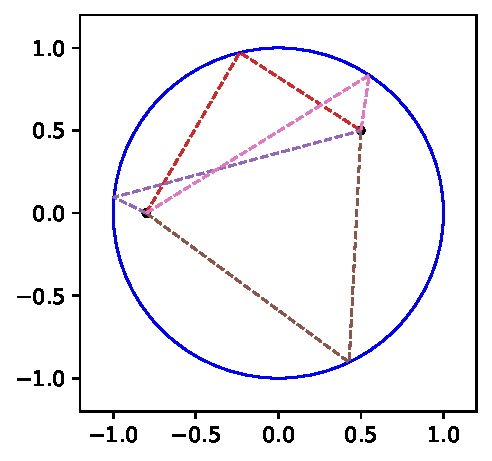
\includegraphics{ADOneDimManually_files/figure-pdf/fig-billardproblemsolution-output-1.pdf}

}

\caption{\label{fig-billardproblemsolution}Lösung des Billardproblems.}

\end{figure}

\end{tcolorbox}

In den folgenden beiden Aufgaben wollen wir das Gradient Descent
Verfahren aus Kapitel~\ref{sec-gradientDescent} anwenden, um eine
Funktion zu minimieren. Auch hier nutzen wir aus, dass uns der
Funktionsaufruf jeweils den exakten Wert der Ableitung mitliefert.

\begin{exercise}[Minimale Kosten mit Gradient
Descent]\protect\hypertarget{exr-MinKosten}{}\label{exr-MinKosten}

Benutze das Gradient Descent Verfahren, um das Minimum der Funktion
\texttt{kosten(x)} aus Übungsaufgabe~\ref{exr-SADKostenfunktionManuell}
zu bestimmen. Starte bei \texttt{x0\ =\ 8} und führe die Iteration so
lange aus, bis sich zwei aufeinanderfolgende Werte um nicht mehr als
eine bestimmte Toleranz, z.B. \texttt{tol\ =\ 1e-4}. Experimentiere mit
verschiedenen Werten für \(\lambda\)

\end{exercise}

\begin{tcolorbox}[enhanced jigsaw, titlerule=0mm, title=\textcolor{quarto-callout-tip-color}{\faLightbulb}\hspace{0.5em}{Lösung}, breakable, coltitle=black, leftrule=.75mm, bottomrule=.15mm, colback=white, rightrule=.15mm, opacitybacktitle=0.6, bottomtitle=1mm, toptitle=1mm, left=2mm, toprule=.15mm, colbacktitle=quarto-callout-tip-color!10!white, colframe=quarto-callout-tip-color-frame, arc=.35mm, opacityback=0]

\begin{Shaded}
\begin{Highlighting}[]
\ImportTok{import}\NormalTok{ math}

\KeywordTok{def}\NormalTok{ kosten(x):}
\NormalTok{    v0dot }\OperatorTok{=} \DecValTok{1}
\NormalTok{    v0 }\OperatorTok{=}\NormalTok{ x       }\CommentTok{\# sX}
\NormalTok{    v1dot }\OperatorTok{=} \OperatorTok{{-}}\NormalTok{v0dot}
\NormalTok{    v1 }\OperatorTok{=} \DecValTok{16} \OperatorTok{{-}}\NormalTok{ v0 }\CommentTok{\# d}
\NormalTok{    v2dot }\OperatorTok{=} \DecValTok{2}\OperatorTok{*}\NormalTok{v1 }\OperatorTok{*}\NormalTok{ v1dot}
\NormalTok{    v2 }\OperatorTok{=}\NormalTok{ v1}\OperatorTok{**}\DecValTok{2} \OperatorTok{+} \DecValTok{12}\OperatorTok{**}\DecValTok{2}
\NormalTok{    v3dot }\OperatorTok{=} \DecValTok{1}\OperatorTok{/}\NormalTok{(}\DecValTok{2}\OperatorTok{*}\NormalTok{math.sqrt(v2)) }\OperatorTok{*}\NormalTok{ v2dot}
\NormalTok{    v3 }\OperatorTok{=}\NormalTok{ math.sqrt(v2) }\CommentTok{\# sLand}
\NormalTok{    v4dot }\OperatorTok{=} \DecValTok{15000} \OperatorTok{*}\NormalTok{ v0dot}
\NormalTok{    v4 }\OperatorTok{=} \DecValTok{15000} \OperatorTok{*}\NormalTok{ v0 }\CommentTok{\# kKueste}
\NormalTok{    v5dot }\OperatorTok{=} \DecValTok{25000} \OperatorTok{*}\NormalTok{ v3dot}
\NormalTok{    v5 }\OperatorTok{=} \DecValTok{25000} \OperatorTok{*}\NormalTok{ v3 }\CommentTok{\# kLand}
\NormalTok{    ydot }\OperatorTok{=}\NormalTok{ v4dot }\OperatorTok{+}\NormalTok{ v5dot}
\NormalTok{    y }\OperatorTok{=}\NormalTok{ v4 }\OperatorTok{+}\NormalTok{ v5}
    \ControlFlowTok{return}\NormalTok{ [y, ydot]}

\NormalTok{x0 }\OperatorTok{=} \DecValTok{8}
\NormalTok{lam }\OperatorTok{=} \FloatTok{0.0001}
\NormalTok{tol }\OperatorTok{=} \FloatTok{1e{-}4}
\CommentTok{\# 1. Schritt}
\NormalTok{[k, kdot] }\OperatorTok{=}\NormalTok{ kosten(x0)}
\NormalTok{x1 }\OperatorTok{=}\NormalTok{ x0 }\OperatorTok{{-}}\NormalTok{ lam }\OperatorTok{*}\NormalTok{ kdot}
\ControlFlowTok{while}\NormalTok{ math.fabs(x1 }\OperatorTok{{-}}\NormalTok{ x0) }\OperatorTok{\textgreater{}}\NormalTok{ tol:}
\NormalTok{    x0 }\OperatorTok{=}\NormalTok{ x1}
\NormalTok{    [k, kdot] }\OperatorTok{=}\NormalTok{ kosten(x0)}
\NormalTok{    x1 }\OperatorTok{=}\NormalTok{ x0 }\OperatorTok{{-}}\NormalTok{ lam }\OperatorTok{*}\NormalTok{ kdot}
\BuiltInTok{print}\NormalTok{(}\StringTok{"Bei x ="}\NormalTok{, x1, }\StringTok{"sind die Kosten minimal."}\NormalTok{)}
\BuiltInTok{print}\NormalTok{(}\StringTok{"Sie belaufen sich auf"}\NormalTok{, k)}
\end{Highlighting}
\end{Shaded}

\begin{verbatim}
Bei x = 7.000767589818459 sind die Kosten minimal.
Sie belaufen sich auf 480000.000393777
\end{verbatim}

\end{tcolorbox}

\begin{exercise}[Minimaler
Abstand]\protect\hypertarget{exr-MinDistlSolution}{}\label{exr-MinDistlSolution}

Leite das Programm aus Beispiel~\ref{exm-GDApplication} ab. Schreibe
danach eine Funktion \texttt{gradient\_descent(f,\ x0,\ lam)}, welche
ausnutzt, dass der Funktionsaufruf \texttt{f(x0)} auch den exakten Wert
der Ableitung zurückgibt. Stelle die gefundene Lösung grafisch dar.

\end{exercise}

\begin{tcolorbox}[enhanced jigsaw, titlerule=0mm, title=\textcolor{quarto-callout-tip-color}{\faLightbulb}\hspace{0.5em}{Lösung}, breakable, coltitle=black, leftrule=.75mm, bottomrule=.15mm, colback=white, rightrule=.15mm, opacitybacktitle=0.6, bottomtitle=1mm, toptitle=1mm, left=2mm, toprule=.15mm, colbacktitle=quarto-callout-tip-color!10!white, colframe=quarto-callout-tip-color-frame, arc=.35mm, opacityback=0]

\begin{Shaded}
\begin{Highlighting}[]
\ImportTok{import}\NormalTok{ math}
\ImportTok{import}\NormalTok{ matplotlib.pyplot }\ImportTok{as}\NormalTok{ plt}

\KeywordTok{def}\NormalTok{ d(t):}
\NormalTok{    v0dot }\OperatorTok{=} \DecValTok{1}                    
\NormalTok{    v0 }\OperatorTok{=}\NormalTok{ t}
\NormalTok{    v1dot }\OperatorTok{=} \OperatorTok{{-}}\DecValTok{2} \OperatorTok{*}\NormalTok{ math.sin(v0) }\OperatorTok{*}\NormalTok{ v0dot   }\CommentTok{\# Ableitung von...}
\NormalTok{    v1 }\OperatorTok{=} \DecValTok{2} \OperatorTok{*}\NormalTok{ math.cos(v0) }\OperatorTok{{-}} \DecValTok{1}    \CommentTok{\# x{-}Koordinate von P}
\NormalTok{    v2dot }\OperatorTok{=} \FloatTok{1.5} \OperatorTok{*}\NormalTok{ math.cos(v0) }\OperatorTok{*}\NormalTok{ v0dot  }\CommentTok{\# Ableitung von...}
\NormalTok{    v2 }\OperatorTok{=} \FloatTok{1.5} \OperatorTok{*}\NormalTok{ math.sin(v0)      }\CommentTok{\# y{-}Koordinate von P}
\NormalTok{    v3dot }\OperatorTok{=} \DecValTok{0}                    \CommentTok{\# Ableitung von...}
\NormalTok{    v3 }\OperatorTok{=} \DecValTok{0}                       \CommentTok{\# z{-}Koordinate von P}
\NormalTok{    v4dot }\OperatorTok{=} \OperatorTok{{-}}\DecValTok{6} \OperatorTok{*}\NormalTok{ math.cos(}\DecValTok{2}\OperatorTok{*}\NormalTok{v0) }\OperatorTok{*}\NormalTok{ v0dot }\CommentTok{\# Ableitung von...}
\NormalTok{    v4 }\OperatorTok{=} \OperatorTok{{-}}\DecValTok{3} \OperatorTok{*}\NormalTok{ math.sin(}\DecValTok{2}\OperatorTok{*}\NormalTok{v0)     }\CommentTok{\# x{-}Koordinate von Q}
\NormalTok{    v5dot }\OperatorTok{=} \OperatorTok{{-}}\DecValTok{4} \OperatorTok{*}\NormalTok{ math.sin(}\DecValTok{2}\OperatorTok{*}\NormalTok{v0) }\OperatorTok{*}\NormalTok{ v0dot }\CommentTok{\# Ableitung von...}
\NormalTok{    v5 }\OperatorTok{=} \DecValTok{2} \OperatorTok{*}\NormalTok{ math.cos(}\DecValTok{2}\OperatorTok{*}\NormalTok{v0) }\OperatorTok{+} \DecValTok{1}  \CommentTok{\# y{-}Koordinate von Q}
\NormalTok{    v6dot }\OperatorTok{=} \DecValTok{4} \OperatorTok{*}\NormalTok{ math.cos(}\DecValTok{2}\OperatorTok{*}\NormalTok{v0) }\OperatorTok{*}\NormalTok{ v0dot  }\CommentTok{\# Ableitung von...}
\NormalTok{    v6 }\OperatorTok{=} \DecValTok{2} \OperatorTok{*}\NormalTok{ math.sin(}\DecValTok{2}\OperatorTok{*}\NormalTok{v0) }\OperatorTok{+} \DecValTok{1}  \CommentTok{\# z{-}Koordinate von Q}
\NormalTok{    ydot }\OperatorTok{=}\NormalTok{ (}\DecValTok{2}\OperatorTok{*}\NormalTok{(v4}\OperatorTok{{-}}\NormalTok{v1)}\OperatorTok{*}\NormalTok{(v4dot}\OperatorTok{{-}}\NormalTok{v1dot) }\OperatorTok{+} \DecValTok{2}\OperatorTok{*}\NormalTok{(v5}\OperatorTok{{-}}\NormalTok{v2)}\OperatorTok{*}\NormalTok{(v5dot}\OperatorTok{{-}}\NormalTok{v2dot) }\OperatorTok{+} \DecValTok{2}\OperatorTok{*}\NormalTok{(v6}\OperatorTok{{-}}\NormalTok{v3)}\OperatorTok{*}\NormalTok{(v6dot}\OperatorTok{{-}}\NormalTok{v3dot)) }\OperatorTok{\textbackslash{}}
         \OperatorTok{/}\NormalTok{ (}\DecValTok{2} \OperatorTok{*}\NormalTok{ math.sqrt((v4}\OperatorTok{{-}}\NormalTok{v1)}\OperatorTok{**}\DecValTok{2} \OperatorTok{+}\NormalTok{ (v5}\OperatorTok{{-}}\NormalTok{v2)}\OperatorTok{**}\DecValTok{2} \OperatorTok{+}\NormalTok{ (v6}\OperatorTok{{-}}\NormalTok{v3)}\OperatorTok{**}\DecValTok{2}\NormalTok{))}
\NormalTok{    y }\OperatorTok{=}\NormalTok{ math.sqrt((v4}\OperatorTok{{-}}\NormalTok{v1)}\OperatorTok{**}\DecValTok{2} \OperatorTok{+}\NormalTok{ (v5}\OperatorTok{{-}}\NormalTok{v2)}\OperatorTok{**}\DecValTok{2} \OperatorTok{+}\NormalTok{ (v6}\OperatorTok{{-}}\NormalTok{v3)}\OperatorTok{**}\DecValTok{2}\NormalTok{)}
    \ControlFlowTok{return}\NormalTok{ [y, ydot]}

\KeywordTok{def}\NormalTok{ gradient\_descent(f, x0, lam):}
\NormalTok{    tol }\OperatorTok{=} \FloatTok{1e{-}9}
    \CommentTok{\# Erster Schritt berechnen}
\NormalTok{    [y0, y0dot] }\OperatorTok{=}\NormalTok{ f(x0)}
\NormalTok{    x1 }\OperatorTok{=}\NormalTok{ x0 }\OperatorTok{{-}}\NormalTok{ lam }\OperatorTok{*}\NormalTok{ y0dot}
    \ControlFlowTok{while}\NormalTok{ math.fabs(x1}\OperatorTok{{-}}\NormalTok{x0) }\OperatorTok{\textgreater{}}\NormalTok{ tol:}
\NormalTok{        x0 }\OperatorTok{=}\NormalTok{ x1}
\NormalTok{        [y0, y0dot] }\OperatorTok{=}\NormalTok{ f(x0)}
\NormalTok{        x1 }\OperatorTok{=}\NormalTok{ x0 }\OperatorTok{{-}}\NormalTok{ lam }\OperatorTok{*}\NormalTok{ y0dot}
    \ControlFlowTok{return}\NormalTok{ x1}

\ControlFlowTok{if} \VariableTok{\_\_name\_\_} \OperatorTok{==} \StringTok{"\_\_main\_\_"}\NormalTok{:}
\NormalTok{    t0 }\OperatorTok{=} \DecValTok{3}
\NormalTok{    tmin }\OperatorTok{=}\NormalTok{ gradient\_descent(d, t0, }\FloatTok{0.01}\NormalTok{)}
\NormalTok{    [dmin, dmindot] }\OperatorTok{=}\NormalTok{ d(tmin)}
    \BuiltInTok{print}\NormalTok{(}\StringTok{"Minimum bei ("}\NormalTok{, tmin, dmin, }\StringTok{")"}\NormalTok{)}

\NormalTok{    fig }\OperatorTok{=}\NormalTok{ plt.figure()}
\NormalTok{    ax }\OperatorTok{=}\NormalTok{ plt.gca()}
\NormalTok{    ax.set\_xlim((}\DecValTok{0}\NormalTok{,}\DecValTok{2}\OperatorTok{*}\NormalTok{math.pi))}
\NormalTok{    ax.set\_ylim((}\DecValTok{0}\NormalTok{,}\DecValTok{6}\NormalTok{))}
\NormalTok{    T }\OperatorTok{=}\NormalTok{ [}\DecValTok{2}\OperatorTok{*}\NormalTok{math.pi }\OperatorTok{*}\NormalTok{ k }\OperatorTok{/} \DecValTok{1000} \ControlFlowTok{for}\NormalTok{ k }\KeywordTok{in} \BuiltInTok{range}\NormalTok{(}\DecValTok{1001}\NormalTok{)]}
\NormalTok{    Y }\OperatorTok{=}\NormalTok{ [d(t)[}\DecValTok{0}\NormalTok{] }\ControlFlowTok{for}\NormalTok{ t }\KeywordTok{in}\NormalTok{ T]  }\CommentTok{\# nur Funktionswert plotten}
\NormalTok{    plt.plot(T,Y)}
\NormalTok{    plt.xticks([}\DecValTok{0}\NormalTok{, math.pi}\OperatorTok{/}\DecValTok{2}\NormalTok{, math.pi, }\DecValTok{3}\OperatorTok{*}\NormalTok{math.pi}\OperatorTok{/}\DecValTok{2}\NormalTok{, }\DecValTok{2}\OperatorTok{*}\NormalTok{math.pi],}
\NormalTok{               [}\StringTok{\textquotesingle{}0\textquotesingle{}}\NormalTok{, }\StringTok{\textquotesingle{}π/2\textquotesingle{}}\NormalTok{, }\StringTok{\textquotesingle{}π\textquotesingle{}}\NormalTok{, }\StringTok{\textquotesingle{}3π/2\textquotesingle{}}\NormalTok{, }\StringTok{\textquotesingle{}2π\textquotesingle{}}\NormalTok{])}
\NormalTok{    plt.plot(tmin,dmin,color}\OperatorTok{=}\StringTok{\textquotesingle{}r\textquotesingle{}}\NormalTok{, marker}\OperatorTok{=}\StringTok{\textquotesingle{}o\textquotesingle{}}\NormalTok{)}
\NormalTok{    plt.show()      }
\end{Highlighting}
\end{Shaded}

\begin{verbatim}
Minimum bei ( 4.712388977478413 1.5 )
\end{verbatim}

\begin{figure}[H]

{\centering 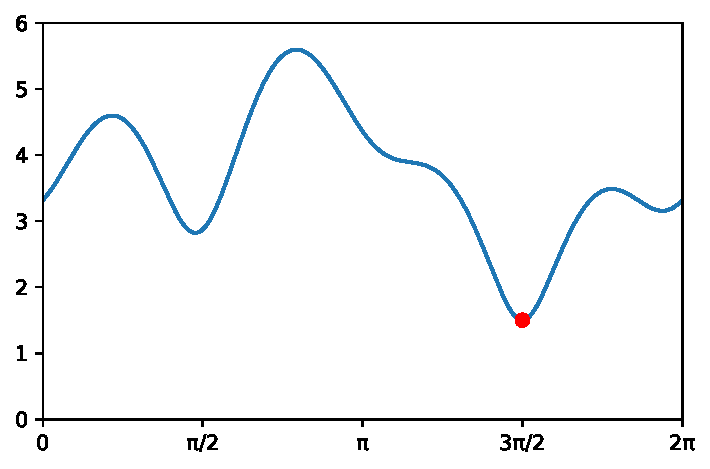
\includegraphics{ADOneDimManually_files/figure-pdf/fig-mindistproblemsolution-output-2.pdf}

}

\caption{\label{fig-mindistproblemsolution}Kürzester Abstand mit
Gradient Descent.}

\end{figure}

Beachte, dass beim Zeichnen des Funktionsgraphen neu
\texttt{Y\ =\ {[}d(t){[}0{]}\ for\ t\ in\ T{]}} steht. Der Grund dafür
ist, dass \texttt{d(t)} nun eine Liste mit zwei Elementen ist
(Funktionswert und Ableitung) und wir nur den Funktionswert zeichnen
wollen. Schreibt man stattdessen
\texttt{Y\ =\ {[}d(t)\ for\ t\ in\ T{]}}, dann wird zusätzlich auch der
Graph der Ableitung gezeichnet.

\end{tcolorbox}

\hypertarget{sec-SadImplementationOperatorOverloading}{%
\section{Implementation der SAD mit Operator
Overloading}\label{sec-SadImplementationOperatorOverloading}}

Nach dem letzten Abschnitt könnte man einwenden, dass wir die
Ableitungen der Funktionen ja doch von Hand berechnet haben, denn wir
haben jede Programmzeile, in der eine Variable \texttt{v} berechnet
wird, um eine weitere Zeile ergänzt, in der wir \texttt{vdot} nach den
bekannten Ableitungsregeln berechnet haben. Dieser Einwand ist auch
berechtigt - oder wie es Henrard ausdrückt:

\begin{quote}
``The bad news is that it {[}calculating the derivatives{]} has to be
done; it will not appear magically. It is not only a figure of speech
that `something has to be done' but that to have it working everything
has to be done''. (Henrard 2017, 17)
\end{quote}

Die gute Nachricht ist, dass wir diesen Prozess weiter automatisieren
können. Wir kennen die Ableitungsregeln für die elementaren Operationen
(\texttt{+,-,*,/}), sowie für die Grundfunktionen. In diesem Abschnitt
werden wir eine Klasse \texttt{FloatSad} schreiben, deren Instanzen
Funktionswerte und Werte der Ableitung speichern. Da solche Werte in der
Regel vom Typ \texttt{float} sind und wir die Standard-AD
implementieren, nennen wir die Klasse \texttt{FloatSad}. Die Arbeit
besteht dann darin, die Ableitungsregeln richtig in den Operatoren
dieser Klasse zu kodieren. Da Python \emph{Operator Overloading} kennt,
werden wir dann nach getaner Arbeit die Ableitungen wirklich ohne
zusätzlichen Programmieraufwand erhalten.

Der Grundstein für unsere Klasse wurde bereits im 19. Jahrhundert
gelegt, wie die folgende Infobox zeigt:

\begin{tcolorbox}[enhanced jigsaw, titlerule=0mm, title=\textcolor{quarto-callout-note-color}{\faInfo}\hspace{0.5em}{Hintergrund: Duale Zahlen}, breakable, coltitle=black, leftrule=.75mm, bottomrule=.15mm, colback=white, rightrule=.15mm, opacitybacktitle=0.6, bottomtitle=1mm, toptitle=1mm, left=2mm, toprule=.15mm, colbacktitle=quarto-callout-note-color!10!white, colframe=quarto-callout-note-color-frame, arc=.35mm, opacityback=0]

Duale Zahlen wurden 1873 durch William Clifford eingeführt und sind
ähnlich definiert, wie komplexe Zahlen. Zur Erinnerung: Eine komplexe
Zahl ist eine Zahl der Form \(a + bi\), wobei \(a,b \in \mathbb{R}\)
sind und \(i\) die Eigenschaft \(i^2 = -1\) hat. Eine duale Zahl ist
eine Zahl der Form \(a + a'\epsilon\), wobei wieder
\(a,a' \in \mathbb{R}\) gilt, aber \(\epsilon\) die Eigenschaft
\(\epsilon^2 = 0\) hat. Nun kann man nach dem Permanenzprinzip die
folgenden Operationen für duale Zahlen definieren:

\begin{alignat*}{3}
    &\textrm{Addition:} && (a+a'\epsilon) + (b+b'\epsilon) &&= (a+b) + (a'+b')\epsilon \\ \\
    &\textrm{Subtraktion:} && (a+a'\epsilon) - (b+b'\epsilon) &&= (a-b) + (a'-b')\epsilon \\ \\
    &\textrm{Multiplikation:}\quad && (a+a'\epsilon) \cdot (b+b'\epsilon) &&= ab + a'b\epsilon + ab'\epsilon + a'b'\epsilon^2 \\
    & && &&= ab + (a'b + ab')\epsilon \\ \\
    &\textrm{Division:} && (\textrm{für }b\ne 0) \quad \frac{a+a'\epsilon}{b+b'\epsilon} &&= \frac{(a+a'\epsilon)(b-b'\epsilon)}{(b+b'\epsilon)(b-b'\epsilon)} \\
    & && &&= \frac{ab+a'b\epsilon-ab'\epsilon-a'b'\epsilon^2}{b^2 - (b')^2\epsilon^2} \\ 
    & && &&= \frac{ab + (a'b-ab')\epsilon}{b^2} \\ 
    & && &&= \frac{a}{b} + \frac{a'b - ab'}{b^2} \epsilon
\end{alignat*}

Wir sehen, dass der reelle Teil den Wert der Operation und der duale
Teil den Wert der zugehörigen Ableitung enthält. Dies gilt auch für
Potenzen, wie man unter Anwendung des binomischen Satzes sieht:

\begin{align*}
    (a+a'\epsilon)^n &= \sum_{k=0}^n \binom n k a^{n-k} (a'\epsilon)^k  \\
    &= a^n + n \cdot a^{n-1} \cdot a'\epsilon + (\textrm{Terme mit }\epsilon^2) \\ 
    &= a^n + n \cdot a^{n-1} \cdot a' \epsilon
\end{align*}

Im dualen Teil erkennen wir die Kettenregel
\((a^n)' = n\cdot a^{n-1}\cdot a'\). Damit können wir duale Zahlen auch
in Polynome \(p(x) = p_0 + p_1 x + p_2 x^2 + \ldots + p_n x^n\)
einsetzen. Wir erhalten dann

\begin{align*}
    p(a+a'\epsilon) &= p_0 + p_1 (a+a'\epsilon) + p_2 (a+a'\epsilon)^2 + \ldots + p_n (a+a'\epsilon)^n \\ 
    &= p_0 + p_1 a + p_1 a'\epsilon + p_2 a^2 + p_2 \cdot 2a a' \epsilon + ... + p_n a^n + p_n \cdot n a^{n-1} a' \epsilon \\ 
    &= p_0 + p_1 a + p_2 a^2 + \ldots p_n a^n + (p_1 + p_2 \cdot 2a + \ldots + p_n \cdot n a^{n-1}) \cdot a' \epsilon \\
    &= p(a) + p'(a) \cdot a'\epsilon
\end{align*}

Dieses Resultat lässt sich auf allgemeine Funktionen \(f\)
verallgemeinern (für den Beweis entwickelt man \(f\) in eine Taylorreihe
und macht die gleichen Überlegungen wie für ein Polynom): \[
f(a+a'\epsilon) = f(a) + f'(a)\cdot a'\epsilon
\]

(\href{https://en.wikipedia.org/wiki/Dual_number}{Wikipedia: Dual
number} und Slater (2022))

\end{tcolorbox}

\hypertarget{sec-FoatSadClassDescription}{%
\subsection{\texorpdfstring{Die Klasse
\texttt{FloatSad}}{Die Klasse FloatSad}}\label{sec-FoatSadClassDescription}}

Beginnen wir nun mit der Implementation unserer Klasse
\texttt{FloatSad}. Analog zu den dualen Zahlen enthält jedes
\texttt{FloatSad}-Objekt zwei Attribute. Das Attribut \texttt{value}
speichert den Funktionswert und das Attribut \texttt{derivative}
speichert den Wert der Ableitung. Im Konstruktor der Klasse setzen wir
für \texttt{derivative} den Standardwert \texttt{1}. Damit können wir
eine gewöhnliche \texttt{Float}-Zahl korrekt in ein \texttt{FloatSad}
umwandeln. Dies wird im \texttt{main} Programm demonstriert.

\begin{Shaded}
\begin{Highlighting}[]
\ImportTok{import}\NormalTok{ math}

\KeywordTok{class}\NormalTok{ FloatSad:}

    \KeywordTok{def} \FunctionTok{\_\_init\_\_}\NormalTok{(}\VariableTok{self}\NormalTok{, value, derivative }\OperatorTok{=} \FloatTok{1.0}\NormalTok{):}
        \VariableTok{self}\NormalTok{.value }\OperatorTok{=} \BuiltInTok{float}\NormalTok{(value)}
        \VariableTok{self}\NormalTok{.derivative }\OperatorTok{=}\NormalTok{ derivative}


\ControlFlowTok{if} \VariableTok{\_\_name\_\_} \OperatorTok{==} \StringTok{\textquotesingle{}\_\_main\_\_\textquotesingle{}}\NormalTok{:}

    \KeywordTok{def}\NormalTok{ f(x):}
\NormalTok{        v0 }\OperatorTok{=}\NormalTok{ FloatSad(x)}
\NormalTok{        y }\OperatorTok{=}\NormalTok{ v0}
        \ControlFlowTok{return}\NormalTok{ y}

\NormalTok{    x0 }\OperatorTok{=} \DecValTok{2}
\NormalTok{    resultat }\OperatorTok{=}\NormalTok{ f(x0)}
    \BuiltInTok{print}\NormalTok{(}\StringTok{"Funktionswert:"}\NormalTok{, resultat.value)}
    \BuiltInTok{print}\NormalTok{(}\StringTok{"Ableitung:"}\NormalTok{, resultat.derivative)}
\end{Highlighting}
\end{Shaded}

\begin{verbatim}
Funktionswert: 2.0
Ableitung: 1.0
\end{verbatim}

In der Funktion \texttt{f} haben wir nun unsere Konvention, dass
\texttt{v0\ =\ x} sein soll, dazu verwendet, den Zahlenwert \texttt{x}
in ein \texttt{FloatSad}-Objekt umzuwandeln. Die Konvention
\texttt{v0dot\ =\ 1} ist im Konstruktor kodiert. Von nun an machen wir
also die folgende Konvention:

\begin{tcolorbox}[enhanced jigsaw, titlerule=0mm, title=\textcolor{quarto-callout-important-color}{\faExclamation}\hspace{0.5em}{Konvention}, breakable, coltitle=black, leftrule=.75mm, bottomrule=.15mm, colback=white, rightrule=.15mm, opacitybacktitle=0.6, bottomtitle=1mm, toptitle=1mm, left=2mm, toprule=.15mm, colbacktitle=quarto-callout-important-color!10!white, colframe=quarto-callout-important-color-frame, arc=.35mm, opacityback=0]

Eine Funktion berechnet aus einem Argument \texttt{x} vom Typ
\texttt{float} oder \texttt{int} einen Rückgabewert \texttt{y} vom Typ
\texttt{FloatSad} über eine Reihe von Hilfsvariablen \texttt{v}, die
alle vom Typ \texttt{FloatSad} sind. Insbesondere setzen wir am Anfang
immer \texttt{v0\ =\ FloatSad(x)}.

\end{tcolorbox}

Das obige Programm berechnet also den Funktionswert und den Wert der
Ableitung von \(f(x) = x\) an der Stelle \(x_0 = 2\).

Um die Ausgabe etwas einfacher zu gestalten implementieren wir als
nächstes die \texttt{print} Methode für unsere Klasse. Wir geben ein
\texttt{FloatSad}-Objekt einfach in der Form
\texttt{\textless{}\ value\ ;\ derivative\ \textgreater{}} aus.

\begin{Shaded}
\begin{Highlighting}[]
\KeywordTok{def} \FunctionTok{\_\_repr\_\_}\NormalTok{(}\VariableTok{self}\NormalTok{):}
        \ControlFlowTok{return} \StringTok{"\textless{} "} \OperatorTok{+} \BuiltInTok{str}\NormalTok{(}\VariableTok{self}\NormalTok{.value) }\OperatorTok{+} \StringTok{" ; "} \OperatorTok{+} \BuiltInTok{str}\NormalTok{(}\VariableTok{self}\NormalTok{.derivative) }\OperatorTok{+} \StringTok{" \textgreater{}"}
\end{Highlighting}
\end{Shaded}

Da wir nun die Funktion \(f(x) = x\) programmieren können, wollen wir
als nächstes auch die Funktion \(f(x) = -x\) programmieren können. Wir
müssen unsere \texttt{FloatSad}-Objekte also mit Vorzeichen versehen.

\hypertarget{vorzeichen}{%
\subsection{Vorzeichen}\label{vorzeichen}}

Natürlich wollen wir nicht nur das negative Vorzeichen, sondern auch das
positive Vorzeichen implementieren, damit wir in unseren Programmen z.B.
\texttt{v1\ =\ +v0} oder \texttt{v2\ =\ -v0} schreiben können. Beim
positiven Vorzeichen müssen wir nichts machen, wir geben also ein
\texttt{FloatSad}-Objekt mit den gleichen Attributen zurück. Beim
negativen Vorzeichen ändern beide Attribute ihr Vorzeichen.

\begin{Shaded}
\begin{Highlighting}[]
\KeywordTok{def} \FunctionTok{\_\_pos\_\_}\NormalTok{(}\VariableTok{self}\NormalTok{):}
        \ControlFlowTok{return}\NormalTok{ FloatSad(}\VariableTok{self}\NormalTok{.value, }\VariableTok{self}\NormalTok{.derivative)}
    
\KeywordTok{def} \FunctionTok{\_\_neg\_\_}\NormalTok{(}\VariableTok{self}\NormalTok{):}
\NormalTok{    newValue }\OperatorTok{=} \OperatorTok{{-}}\VariableTok{self}\NormalTok{.value}
\NormalTok{    newDerivative }\OperatorTok{=} \OperatorTok{{-}}\VariableTok{self}\NormalTok{.derivative}
    \ControlFlowTok{return}\NormalTok{ FloatSad(newValue, newDerivative)}
\end{Highlighting}
\end{Shaded}

Nun gehen wir daran, die Grundoperationen für \texttt{FloatSad}-Objekte
zu implementieren.

\hypertarget{sec-implementAddSubtract}{%
\subsection{\texorpdfstring{Die Operatoren \texttt{+} und
\texttt{-}}{Die Operatoren + und -}}\label{sec-implementAddSubtract}}

Wir möchten in unseren Programmen Anweisungen wie
\texttt{v2\ =\ v0\ +\ v1} verwenden können. Gemäss der Summenregel
können wir dazu einfach die Funktionswerte und auch die Werte der
Ableitungen addieren.

\begin{Shaded}
\begin{Highlighting}[]
\KeywordTok{def} \FunctionTok{\_\_add\_\_}\NormalTok{(}\VariableTok{self}\NormalTok{, other):}
\NormalTok{        newValue }\OperatorTok{=} \VariableTok{self}\NormalTok{.value }\OperatorTok{+}\NormalTok{ other.value}
\NormalTok{        newDerivative }\OperatorTok{=} \VariableTok{self}\NormalTok{.derivative }\OperatorTok{+}\NormalTok{ other.derivative}
        \ControlFlowTok{return}\NormalTok{ FloatSad(newValue, newDerivative)}
\end{Highlighting}
\end{Shaded}

Nun können wir zwei \texttt{FloatSad}-Objekte miteinander addieren.
Manchmal möchten wir aber auch ein \texttt{float}- oder
\texttt{int}-Wert zu einem \texttt{FloatSad}-Objekt addieren, z.B.
\texttt{v1\ =\ v0\ +\ 2}. Dazu machen wir eine Typabfrage und passen den
Wert der Ableitung entsprechend der Konstantenregel an:

\begin{Shaded}
\begin{Highlighting}[]
\KeywordTok{def} \FunctionTok{\_\_add\_\_}\NormalTok{(}\VariableTok{self}\NormalTok{, other):}
    \ControlFlowTok{if} \BuiltInTok{type}\NormalTok{(other) }\KeywordTok{in}\NormalTok{ (}\BuiltInTok{float}\NormalTok{, }\BuiltInTok{int}\NormalTok{):}
\NormalTok{        newValue }\OperatorTok{=} \VariableTok{self}\NormalTok{.value }\OperatorTok{+}\NormalTok{ other}
\NormalTok{        newDerivative }\OperatorTok{=} \VariableTok{self}\NormalTok{.derivative }\OperatorTok{+} \FloatTok{0.0}
    \ControlFlowTok{else}\NormalTok{:}
\NormalTok{        newValue }\OperatorTok{=} \VariableTok{self}\NormalTok{.value }\OperatorTok{+}\NormalTok{ other.value}
\NormalTok{        newDerivative }\OperatorTok{=} \VariableTok{self}\NormalTok{.derivative }\OperatorTok{+}\NormalTok{ other.derivative}
    \ControlFlowTok{return}\NormalTok{ FloatSad(newValue, newDerivative)}
\end{Highlighting}
\end{Shaded}

Jetzt funktioniert zwar die Anweisung \texttt{v1\ =\ v0\ +\ 2}, aber die
Anweisung \texttt{v1\ =\ 2\ +\ v0} erzeugt immer noch eine
Fehlermeldung. Um dieses Problem zu beheben, müssen wir als nächstes den
\emph{reverse-add}-Operator implementieren.

\begin{Shaded}
\begin{Highlighting}[]
\KeywordTok{def} \FunctionTok{\_\_radd\_\_}\NormalTok{(}\VariableTok{self}\NormalTok{, other):}
    \ControlFlowTok{if} \BuiltInTok{type}\NormalTok{(other) }\KeywordTok{in}\NormalTok{ (}\BuiltInTok{float}\NormalTok{, }\BuiltInTok{int}\NormalTok{):}
\NormalTok{        newValue }\OperatorTok{=}\NormalTok{ other }\OperatorTok{+} \VariableTok{self}\NormalTok{.value}
\NormalTok{        newDerivative }\OperatorTok{=} \FloatTok{0.0} \OperatorTok{+} \VariableTok{self}\NormalTok{.derivative}
    \ControlFlowTok{else}\NormalTok{:}
\NormalTok{        newValue }\OperatorTok{=}\NormalTok{ other.value }\OperatorTok{+} \VariableTok{self}\NormalTok{.value}
\NormalTok{        newDerivative }\OperatorTok{=}\NormalTok{ other.derivative }\OperatorTok{+} \VariableTok{self}\NormalTok{.derivative}
    \ControlFlowTok{return}\NormalTok{ FloatSad(newValue, newDerivative)}
\end{Highlighting}
\end{Shaded}

Hier ist die bisher implementierte Klasse zusammen mit einem kleinen
Testprogramm.

\begin{Shaded}
\begin{Highlighting}[]
\ImportTok{import}\NormalTok{ math}

\KeywordTok{class}\NormalTok{ FloatSad:}

    \KeywordTok{def} \FunctionTok{\_\_init\_\_}\NormalTok{(}\VariableTok{self}\NormalTok{, value, derivative }\OperatorTok{=} \FloatTok{1.0}\NormalTok{):}
        \VariableTok{self}\NormalTok{.value }\OperatorTok{=} \BuiltInTok{float}\NormalTok{(value)}
        \VariableTok{self}\NormalTok{.derivative }\OperatorTok{=}\NormalTok{ derivative}

    \KeywordTok{def} \FunctionTok{\_\_repr\_\_}\NormalTok{(}\VariableTok{self}\NormalTok{):}
        \ControlFlowTok{return} \StringTok{"\textless{} "} \OperatorTok{+} \BuiltInTok{str}\NormalTok{(}\VariableTok{self}\NormalTok{.value) }\OperatorTok{+} \StringTok{" ; "} \OperatorTok{+} \BuiltInTok{str}\NormalTok{(}\VariableTok{self}\NormalTok{.derivative) }\OperatorTok{+} \StringTok{" \textgreater{}"}


    \CommentTok{\# unäre Operatoren}

    \KeywordTok{def} \FunctionTok{\_\_pos\_\_}\NormalTok{(}\VariableTok{self}\NormalTok{):}
        \ControlFlowTok{return}\NormalTok{ FloatSad(}\VariableTok{self}\NormalTok{.value, }\VariableTok{self}\NormalTok{.derivative)}
    
    \KeywordTok{def} \FunctionTok{\_\_neg\_\_}\NormalTok{(}\VariableTok{self}\NormalTok{):}
\NormalTok{        newValue }\OperatorTok{=} \OperatorTok{{-}}\VariableTok{self}\NormalTok{.value}
\NormalTok{        newDerivative }\OperatorTok{=} \OperatorTok{{-}}\VariableTok{self}\NormalTok{.derivative}
        \ControlFlowTok{return}\NormalTok{ FloatSad(newValue, newDerivative)}
    

    \CommentTok{\# binäre Operatoren}

    \KeywordTok{def} \FunctionTok{\_\_add\_\_}\NormalTok{(}\VariableTok{self}\NormalTok{, other):}
        \ControlFlowTok{if} \BuiltInTok{type}\NormalTok{(other) }\KeywordTok{in}\NormalTok{ (}\BuiltInTok{float}\NormalTok{, }\BuiltInTok{int}\NormalTok{):}
\NormalTok{            newValue }\OperatorTok{=} \VariableTok{self}\NormalTok{.value }\OperatorTok{+}\NormalTok{ other}
\NormalTok{            newDerivative }\OperatorTok{=} \VariableTok{self}\NormalTok{.derivative }\OperatorTok{+} \FloatTok{0.0}
        \ControlFlowTok{else}\NormalTok{:}
\NormalTok{            newValue }\OperatorTok{=} \VariableTok{self}\NormalTok{.value }\OperatorTok{+}\NormalTok{ other.value}
\NormalTok{            newDerivative }\OperatorTok{=} \VariableTok{self}\NormalTok{.derivative }\OperatorTok{+}\NormalTok{ other.derivative}
        \ControlFlowTok{return}\NormalTok{ FloatSad(newValue, newDerivative)}

    \KeywordTok{def} \FunctionTok{\_\_radd\_\_}\NormalTok{(}\VariableTok{self}\NormalTok{, other):}
        \ControlFlowTok{if} \BuiltInTok{type}\NormalTok{(other) }\KeywordTok{in}\NormalTok{ (}\BuiltInTok{float}\NormalTok{, }\BuiltInTok{int}\NormalTok{):}
\NormalTok{            newValue }\OperatorTok{=}\NormalTok{ other }\OperatorTok{+} \VariableTok{self}\NormalTok{.value}
\NormalTok{            newDerivative }\OperatorTok{=} \FloatTok{0.0} \OperatorTok{+} \VariableTok{self}\NormalTok{.derivative}
        \ControlFlowTok{else}\NormalTok{:}
\NormalTok{            newValue }\OperatorTok{=}\NormalTok{ other.value }\OperatorTok{+} \VariableTok{self}\NormalTok{.value}
\NormalTok{            newDerivative }\OperatorTok{=}\NormalTok{ other.derivative }\OperatorTok{+} \VariableTok{self}\NormalTok{.derivative}
        \ControlFlowTok{return}\NormalTok{ FloatSad(newValue, newDerivative)}
    


\ControlFlowTok{if} \VariableTok{\_\_name\_\_} \OperatorTok{==} \StringTok{\textquotesingle{}\_\_main\_\_\textquotesingle{}}\NormalTok{:}

    \KeywordTok{def}\NormalTok{ f(x):}
\NormalTok{        v0 }\OperatorTok{=}\NormalTok{ FloatSad(x)}
\NormalTok{        v1 }\OperatorTok{=} \OperatorTok{{-}}\NormalTok{v0 }
\NormalTok{        v2 }\OperatorTok{=} \DecValTok{3} \OperatorTok{+}\NormalTok{ v1}
\NormalTok{        v3 }\OperatorTok{=}\NormalTok{ v2 }\OperatorTok{+}\NormalTok{ v1}
\NormalTok{        y  }\OperatorTok{=} \OperatorTok{+}\NormalTok{v3}
        \ControlFlowTok{return}\NormalTok{ y}

\NormalTok{    resultat }\OperatorTok{=}\NormalTok{ f(}\DecValTok{2}\NormalTok{)}
    \BuiltInTok{print}\NormalTok{(resultat)}
\end{Highlighting}
\end{Shaded}

\begin{verbatim}
< -1.0 ; -2.0 >
\end{verbatim}

\begin{exercise}[Korrektheit
überprüfen]\protect\hypertarget{exr-verifyFirstSADderivative}{}\label{exr-verifyFirstSADderivative}

Welche Funktion berechnet \texttt{f} im \texttt{main} Programm? Stimmt
die Ausgabe?

\end{exercise}

\begin{tcolorbox}[enhanced jigsaw, titlerule=0mm, title=\textcolor{quarto-callout-tip-color}{\faLightbulb}\hspace{0.5em}{Lösung}, breakable, coltitle=black, leftrule=.75mm, bottomrule=.15mm, colback=white, rightrule=.15mm, opacitybacktitle=0.6, bottomtitle=1mm, toptitle=1mm, left=2mm, toprule=.15mm, colbacktitle=quarto-callout-tip-color!10!white, colframe=quarto-callout-tip-color-frame, arc=.35mm, opacityback=0]

Es handelt sich um die Funktion \(f(x) = 3 - 2x\). Die Ausgabe
\(f(2) = -1, f'(2) = -2\) ist also korrekt.

\end{tcolorbox}

Für die nächste Übung musst du das obige Programm kopieren und in einer
Datei mit dem Namen \texttt{floatsad.py} abspeichern. Speichere die
Datei im gleichen Ordner wie die anderen Dateien.

\begin{exercise}[Den Operator \texttt{-}
implementieren]\protect\hypertarget{exr-ImplementSub}{}\label{exr-ImplementSub}

Implementiere auf die gleiche Weise den \texttt{-}-Operator. Die
Methoden lauten \texttt{\_\_sub\_\_(self,\ other)} bzw.
\texttt{\_\_rsub\_\_(self,\ other)}. Schreibe auch eine Testfunktion
\texttt{f}, welche die neuen Operatoren verwendet.

\end{exercise}

\begin{tcolorbox}[enhanced jigsaw, titlerule=0mm, title=\textcolor{quarto-callout-tip-color}{\faLightbulb}\hspace{0.5em}{Lösung}, breakable, coltitle=black, leftrule=.75mm, bottomrule=.15mm, colback=white, rightrule=.15mm, opacitybacktitle=0.6, bottomtitle=1mm, toptitle=1mm, left=2mm, toprule=.15mm, colbacktitle=quarto-callout-tip-color!10!white, colframe=quarto-callout-tip-color-frame, arc=.35mm, opacityback=0]

\begin{Shaded}
\begin{Highlighting}[]
\KeywordTok{def} \FunctionTok{\_\_sub\_\_}\NormalTok{(}\VariableTok{self}\NormalTok{, other):}
    \ControlFlowTok{if} \BuiltInTok{type}\NormalTok{(other) }\KeywordTok{in}\NormalTok{ (}\BuiltInTok{float}\NormalTok{, }\BuiltInTok{int}\NormalTok{):}
\NormalTok{        newValue }\OperatorTok{=} \VariableTok{self}\NormalTok{.value }\OperatorTok{{-}}\NormalTok{ other}
\NormalTok{        newDerivative }\OperatorTok{=} \VariableTok{self}\NormalTok{.derivative }\OperatorTok{{-}} \FloatTok{0.0}
    \ControlFlowTok{else}\NormalTok{:}
\NormalTok{        newValue }\OperatorTok{=} \VariableTok{self}\NormalTok{.value }\OperatorTok{{-}}\NormalTok{ other.value}
\NormalTok{        newDerivative }\OperatorTok{=} \VariableTok{self}\NormalTok{.derivative }\OperatorTok{{-}}\NormalTok{ other.derivative}
    \ControlFlowTok{return}\NormalTok{ FloatSad(newValue, newDerivative)}

\KeywordTok{def} \FunctionTok{\_\_rsub\_\_}\NormalTok{(}\VariableTok{self}\NormalTok{, other):}
    \ControlFlowTok{if} \BuiltInTok{type}\NormalTok{(other) }\KeywordTok{in}\NormalTok{ (}\BuiltInTok{float}\NormalTok{, }\BuiltInTok{int}\NormalTok{):}
\NormalTok{        newValue }\OperatorTok{=}\NormalTok{ other }\OperatorTok{{-}} \VariableTok{self}\NormalTok{.value}
\NormalTok{        newDerivative }\OperatorTok{=} \FloatTok{0.0} \OperatorTok{{-}} \VariableTok{self}\NormalTok{.derivative}
    \ControlFlowTok{else}\NormalTok{:}
\NormalTok{        newValue }\OperatorTok{=}\NormalTok{ other.value }\OperatorTok{{-}} \VariableTok{self}\NormalTok{.value}
\NormalTok{        newDerivative }\OperatorTok{=}\NormalTok{ other.derivative }\OperatorTok{{-}} \VariableTok{self}\NormalTok{.derivative}
    \ControlFlowTok{return}\NormalTok{ FloatSad(newValue, newDerivative)}
\end{Highlighting}
\end{Shaded}

\end{tcolorbox}

\hypertarget{die-operatoren-und}{%
\subsection{\texorpdfstring{Die Operatoren \texttt{*} und
\texttt{/}}{Die Operatoren * und /}}\label{die-operatoren-und}}

Als nächstes wollen wir die Multiplikation implementieren, um
Anweisungen der Form \texttt{v2\ =\ v0\ *\ v1} ausführen zu können. Dazu
müssen wir die Produktregel verwenden. Wie bei der Addition und der
Subtraktion soll unser \texttt{*}-Operator aber auch Anweisungen der
Form \texttt{v1\ =\ v0\ *\ 2} oder \texttt{v1\ =\ -3\ *\ v0} richtig
auswerten, bei denen die Faktorregel angewendet wird. Dazu ist wieder
eine Typabfrage nötig.

\begin{exercise}[Den Operator \texttt{*}
implementieren]\protect\hypertarget{exr-ImplementMul}{}\label{exr-ImplementMul}

Ergänze die Datei \texttt{floatsad.py} mit den Methoden
\texttt{\_\_mul\_\_(self,\ other)} und
\texttt{\_\_rmul\_\_(self,\ other)}. Überlege dir verschiedene Testfälle
und überzeuge dich von der Korrektheit deines Programms.

\end{exercise}

\begin{tcolorbox}[enhanced jigsaw, titlerule=0mm, title=\textcolor{quarto-callout-tip-color}{\faLightbulb}\hspace{0.5em}{Lösung}, breakable, coltitle=black, leftrule=.75mm, bottomrule=.15mm, colback=white, rightrule=.15mm, opacitybacktitle=0.6, bottomtitle=1mm, toptitle=1mm, left=2mm, toprule=.15mm, colbacktitle=quarto-callout-tip-color!10!white, colframe=quarto-callout-tip-color-frame, arc=.35mm, opacityback=0]

\begin{Shaded}
\begin{Highlighting}[]
\KeywordTok{def} \FunctionTok{\_\_mul\_\_}\NormalTok{(}\VariableTok{self}\NormalTok{, other):}
    \ControlFlowTok{if} \BuiltInTok{type}\NormalTok{(other) }\KeywordTok{in}\NormalTok{ (}\BuiltInTok{float}\NormalTok{, }\BuiltInTok{int}\NormalTok{):}
\NormalTok{        newValue }\OperatorTok{=} \VariableTok{self}\NormalTok{.value }\OperatorTok{*}\NormalTok{ other}
\NormalTok{        newDerivative }\OperatorTok{=} \VariableTok{self}\NormalTok{.derivative }\OperatorTok{*}\NormalTok{ other}
    \ControlFlowTok{else}\NormalTok{:}
\NormalTok{        newValue }\OperatorTok{=} \VariableTok{self}\NormalTok{.value }\OperatorTok{*}\NormalTok{ other.value}
\NormalTok{        newDerivative }\OperatorTok{=} \VariableTok{self}\NormalTok{.derivative }\OperatorTok{*}\NormalTok{ other.value }\OperatorTok{+} \VariableTok{self}\NormalTok{.value }\OperatorTok{*}\NormalTok{ other.derivative}
    \ControlFlowTok{return}\NormalTok{ FloatSad(newValue, newDerivative)}

\KeywordTok{def} \FunctionTok{\_\_rmul\_\_}\NormalTok{(}\VariableTok{self}\NormalTok{, other):}
    \ControlFlowTok{if} \BuiltInTok{type}\NormalTok{(other) }\KeywordTok{in}\NormalTok{ (}\BuiltInTok{float}\NormalTok{, }\BuiltInTok{int}\NormalTok{):}
\NormalTok{        newValue }\OperatorTok{=}\NormalTok{ other }\OperatorTok{*} \VariableTok{self}\NormalTok{.value}
\NormalTok{        newDerivative }\OperatorTok{=}\NormalTok{ other }\OperatorTok{*} \VariableTok{self}\NormalTok{.derivative}
    \ControlFlowTok{else}\NormalTok{:}
\NormalTok{        newValue }\OperatorTok{=}\NormalTok{ other.value }\OperatorTok{*} \VariableTok{self}\NormalTok{.value}
\NormalTok{        newDerivative }\OperatorTok{=}\NormalTok{  other.derivative }\OperatorTok{*} \VariableTok{self}\NormalTok{.value }\OperatorTok{+}\NormalTok{ other.value }\OperatorTok{*} \VariableTok{self}\NormalTok{.derivative}
    \ControlFlowTok{return}\NormalTok{ FloatSad(newValue, newDerivative)}
\end{Highlighting}
\end{Shaded}

\end{tcolorbox}

Es fehlt noch der Divisionsoperator, damit wir Anweisungen wie
\texttt{v2\ =\ v1\ /\ v0} verwenden können. Da wir es bei
differenzierbaren Funktionen immer mit \texttt{float}- bzw.
\texttt{FloatSad}-Objekten zu tun haben, implementieren wir nur den
\texttt{/}-Operator, also die Funktion
\texttt{\_\_truediv\_\_(self,\ other)} und nicht den
\texttt{//}-Operator. Wir wollen aber wieder die Fallunterscheidung nach
den Typen machen, so dass auch Anweisungen wie \texttt{v1\ =\ v0\ /\ 4}
verwendet werden können. Dabei benötigen wir nur die Faktorregel und
nicht die Quotientenregel. Um schliesslich auch noch
\texttt{v1\ =\ -4\ /\ v0} zu ermöglichen, muss noch
\texttt{\_\_rtruediv\_\_(self,\ other)} implementiert werden. Bei
letzterem darf nicht vergessen werden, dass auch die Kettenregel benutzt
werden muss, denn
\(\frac{dv_1}{dx} = \frac{dv_1}{dv_0}\cdot \frac{dv_0}{dx} = \frac{4}{v_0^2}\cdot v_0'\).
Quadrate kann man mit \texttt{math.pow(value,\ 2)} berechnen. Bei der
Implementierung müssen wir uns übrigens nicht um Fehlerbehandlungen, wie
das Abfangen einer Division durch Null, kümmern, weil diese bereits im
\texttt{/}-Operator, den wir verwenden, implementiert sind.

\begin{exercise}[Den Operator \texttt{/}
implementieren]\protect\hypertarget{exr-ImplementTrueDiv}{}\label{exr-ImplementTrueDiv}

Ergänze die Datei \texttt{floatsad.py} mit den Methoden
\texttt{\_\_truediv\_\_(self,\ other)} und
\texttt{\_\_rtruediv\_\_(self,\ other)}. Überlege dir auch wieder
verschiedene Testfälle und überzeuge dich von der Korrektheit deines
Programms.

\end{exercise}

\begin{tcolorbox}[enhanced jigsaw, titlerule=0mm, title=\textcolor{quarto-callout-tip-color}{\faLightbulb}\hspace{0.5em}{Lösung}, breakable, coltitle=black, leftrule=.75mm, bottomrule=.15mm, colback=white, rightrule=.15mm, opacitybacktitle=0.6, bottomtitle=1mm, toptitle=1mm, left=2mm, toprule=.15mm, colbacktitle=quarto-callout-tip-color!10!white, colframe=quarto-callout-tip-color-frame, arc=.35mm, opacityback=0]

\begin{Shaded}
\begin{Highlighting}[]
\KeywordTok{def} \FunctionTok{\_\_truediv\_\_}\NormalTok{(}\VariableTok{self}\NormalTok{, other):}
    \ControlFlowTok{if} \BuiltInTok{type}\NormalTok{(other) }\KeywordTok{in}\NormalTok{ (}\BuiltInTok{float}\NormalTok{, }\BuiltInTok{int}\NormalTok{):}
\NormalTok{        newValue }\OperatorTok{=} \VariableTok{self}\NormalTok{.value }\OperatorTok{/}\NormalTok{ other}
\NormalTok{        newDerivative }\OperatorTok{=} \VariableTok{self}\NormalTok{.derivative }\OperatorTok{/}\NormalTok{ other}
    \ControlFlowTok{else}\NormalTok{:}
\NormalTok{        newValue }\OperatorTok{=} \VariableTok{self}\NormalTok{.value }\OperatorTok{/}\NormalTok{ other.value}
\NormalTok{        newDerivative }\OperatorTok{=}\NormalTok{ (}\VariableTok{self}\NormalTok{.derivative }\OperatorTok{*}\NormalTok{ other.value }\OperatorTok{{-}} \VariableTok{self}\NormalTok{.value }\OperatorTok{*}\NormalTok{ other.derivative) }\OperatorTok{/}\NormalTok{ math.}\BuiltInTok{pow}\NormalTok{(other.value, }\DecValTok{2}\NormalTok{)}
    \ControlFlowTok{return}\NormalTok{ FloatSad(newValue, newDerivative)}

\KeywordTok{def} \FunctionTok{\_\_rtruediv\_\_}\NormalTok{(}\VariableTok{self}\NormalTok{, other):}
    \ControlFlowTok{if} \BuiltInTok{type}\NormalTok{(other) }\KeywordTok{in}\NormalTok{ (}\BuiltInTok{float}\NormalTok{, }\BuiltInTok{int}\NormalTok{):}
\NormalTok{        newValue }\OperatorTok{=}\NormalTok{ other }\OperatorTok{/} \VariableTok{self}\NormalTok{.value}
\NormalTok{        newDerivative }\OperatorTok{=} \OperatorTok{{-}}\NormalTok{ other }\OperatorTok{/}\NormalTok{ math.}\BuiltInTok{pow}\NormalTok{(}\VariableTok{self}\NormalTok{.value, }\DecValTok{2}\NormalTok{) }\OperatorTok{*} \VariableTok{self}\NormalTok{.derivative}
    \ControlFlowTok{else}\NormalTok{:}
\NormalTok{        newValue }\OperatorTok{=}\NormalTok{ other.value }\OperatorTok{/} \VariableTok{self}\NormalTok{.value}
\NormalTok{        newDerivative }\OperatorTok{=}\NormalTok{ (other.derivative }\OperatorTok{*} \VariableTok{self}\NormalTok{.value }\OperatorTok{{-}}\NormalTok{ other.value }\OperatorTok{*} \VariableTok{self}\NormalTok{.derivative) }\OperatorTok{/}\NormalTok{ math.}\BuiltInTok{pow}\NormalTok{(}\VariableTok{self}\NormalTok{.value, }\DecValTok{2}\NormalTok{) }\OperatorTok{*} \VariableTok{self}\NormalTok{.derivative}
    \ControlFlowTok{return}\NormalTok{ FloatSad(newValue, newDerivative)}
\end{Highlighting}
\end{Shaded}

\end{tcolorbox}

\hypertarget{sec-sadPowerOperator}{%
\subsection{\texorpdfstring{Der Operator
\texttt{**}}{Der Operator **}}\label{sec-sadPowerOperator}}

Interessant ist nun die Implementation des Potenzoperators. Hier sind
mehrere Fallunterscheidungen nötig.

Betrachten wir zuerst den Fall, \texttt{type(other)\ in\ (float,\ int)},
d.h. wir haben einen Ausdruck der Form \texttt{v1\ =\ v0\ **\ 3}. In
diesem Fall wenden wir die Potenzregel zusammen mit der Kettenregel an.

Im zweiten Fall haben wir einen Ausdruck wie \texttt{v3\ =\ v1\ **\ v2}.
Wir müssen uns also zuerst überlegen, wie wir einen Ausdruck der Form
\(v_3 (x) = v_1(x) ^{v_2 (x)}\) überhaupt ableiten. Offenbar muss dazu
\(v_1(x) > 0\) gelten. Um die Ableitung zu finden wenden wir den Trick
an, dass wir die Funktion zuerst logarithmieren, \[
\ln(v_3(x)) = \ln(v_1(x) ^{v_2 (x)}) = v_2(x) \cdot \ln(v_1(x))
\] und danach beide Seiten ableiten, wobei wir auf der rechten Seite die
Produktregel anwenden: \[
\frac{d}{dx}(\ln(v_3(x))) = v_2'(x) \cdot \ln(v_1(x)) + v_2(x) \cdot \frac{1}{v_1(x)} \cdot v_1'(x)
\] Die linke Seite ergibt andererseits
\(\frac{d}{dx}(\ln(v_3(x))) = \frac{1}{v_3(x)}\cdot v_3'(x)\), so dass
wir nun nach \(v_3'(x)\) auflösen können:

\begin{align*}
    v_3'(x) &= v_3(x) \cdot \left( v_2'(x) \cdot \ln(v_1(x)) + \frac{v_2(x)}{v_1(x)} \cdot v_1'(x) \right) \\ 
    &= v_1(x) ^{v_2 (x)} \cdot \left( \ln(v_1(x)) \cdot v_2'(x) + \frac{v_2(x)}{v_1(x)} \cdot v_1'(x) \right)
\end{align*}

Auch hier sind alle nötigen Fehlerbehandlungen bereits in
\texttt{math.pow} implementiert.

\begin{exercise}[Den Operator \texttt{**} implementieren - Teil
1]\protect\hypertarget{exr-ImplementPow}{}\label{exr-ImplementPow}

Ergänze die Datei \texttt{floatsad.py} mit der Methode
\texttt{\_\_pow\_\_(self,\ other)}. Dabei übernimmt \texttt{self} die
Rolle von \(v_1\) in der obigen Herleitung und \texttt{other} entspricht
\(v_2\). Die Funktion \(\ln(\ldots)\) heisst in Python
\texttt{math.log()}. Teste dein Programm an verschiedenen Funktionen.

\end{exercise}

\begin{tcolorbox}[enhanced jigsaw, titlerule=0mm, title=\textcolor{quarto-callout-tip-color}{\faLightbulb}\hspace{0.5em}{Lösung}, breakable, coltitle=black, leftrule=.75mm, bottomrule=.15mm, colback=white, rightrule=.15mm, opacitybacktitle=0.6, bottomtitle=1mm, toptitle=1mm, left=2mm, toprule=.15mm, colbacktitle=quarto-callout-tip-color!10!white, colframe=quarto-callout-tip-color-frame, arc=.35mm, opacityback=0]

\begin{Shaded}
\begin{Highlighting}[]
\KeywordTok{def} \FunctionTok{\_\_pow\_\_}\NormalTok{(}\VariableTok{self}\NormalTok{, other):}
    \ControlFlowTok{if} \BuiltInTok{type}\NormalTok{(other) }\KeywordTok{in}\NormalTok{ (}\BuiltInTok{float}\NormalTok{, }\BuiltInTok{int}\NormalTok{):}
\NormalTok{        newValue }\OperatorTok{=}\NormalTok{ math.}\BuiltInTok{pow}\NormalTok{(}\VariableTok{self}\NormalTok{.value, other)}
\NormalTok{        newDerivative }\OperatorTok{=}\NormalTok{ other }\OperatorTok{*}\NormalTok{ math.}\BuiltInTok{pow}\NormalTok{(}\VariableTok{self}\NormalTok{.value, other }\OperatorTok{{-}} \DecValTok{1}\NormalTok{) }\OperatorTok{*} \VariableTok{self}\NormalTok{.derivative}
    \ControlFlowTok{else}\NormalTok{:}
\NormalTok{        newValue }\OperatorTok{=}\NormalTok{ math.}\BuiltInTok{pow}\NormalTok{(}\VariableTok{self}\NormalTok{.value, other.value)}
\NormalTok{        newDerivative }\OperatorTok{=}\NormalTok{ math.}\BuiltInTok{pow}\NormalTok{(}\VariableTok{self}\NormalTok{.value, other.value) }\OperatorTok{*} \OperatorTok{\textbackslash{}}
\NormalTok{            (other.derivative }\OperatorTok{*}\NormalTok{ math.log(}\VariableTok{self}\NormalTok{.value) }\OperatorTok{+}\NormalTok{ other.value }\OperatorTok{*} \VariableTok{self}\NormalTok{.derivative }\OperatorTok{/} \VariableTok{self}\NormalTok{.value)}
    \ControlFlowTok{return}\NormalTok{ FloatSad(newValue, newDerivative)}
\end{Highlighting}
\end{Shaded}

\end{tcolorbox}

Nun implementieren wir auch noch die Methode
\texttt{\_\_rpow\_\_(self,\ other)}. Im Fall, dass
\texttt{type(other)\ in\ (float,\ int)} ist, handelt es sich hierbei um
eine Exponentialfunktion. \texttt{math.pow} stellt dann sicher, dass die
Basis, also \texttt{other}, eine positive Zahl ist. Falls \texttt{other}
ebenfalls ein \texttt{FloatSad} ist, dann kann die Ableitung gleich wie
oben berechnet werden, ausser, dass jetzt \texttt{self} und
\texttt{other} ihre Rollen tauschen.

\begin{exercise}[Den Operator \texttt{**} implementieren - Teil
2]\protect\hypertarget{exr-ImplementRpow}{}\label{exr-ImplementRpow}

Ergänze die Datei \texttt{floatsad.py} mit der Methode
\texttt{\_\_rpow\_\_(self,\ other)}. Teste dein Programm an
verschiedenen Funktionen.

\end{exercise}

\begin{tcolorbox}[enhanced jigsaw, titlerule=0mm, title=\textcolor{quarto-callout-tip-color}{\faLightbulb}\hspace{0.5em}{Lösung}, breakable, coltitle=black, leftrule=.75mm, bottomrule=.15mm, colback=white, rightrule=.15mm, opacitybacktitle=0.6, bottomtitle=1mm, toptitle=1mm, left=2mm, toprule=.15mm, colbacktitle=quarto-callout-tip-color!10!white, colframe=quarto-callout-tip-color-frame, arc=.35mm, opacityback=0]

\begin{Shaded}
\begin{Highlighting}[]
\KeywordTok{def} \FunctionTok{\_\_rpow\_\_}\NormalTok{(}\VariableTok{self}\NormalTok{, other):}
    \ControlFlowTok{if} \BuiltInTok{type}\NormalTok{(other) }\KeywordTok{in}\NormalTok{ (}\BuiltInTok{float}\NormalTok{, }\BuiltInTok{int}\NormalTok{):}
\NormalTok{        newValue }\OperatorTok{=}\NormalTok{ math.}\BuiltInTok{pow}\NormalTok{(other, }\VariableTok{self}\NormalTok{.value)}
\NormalTok{        newDerivative }\OperatorTok{=}\NormalTok{ math.}\BuiltInTok{pow}\NormalTok{(other, }\VariableTok{self}\NormalTok{.value) }\OperatorTok{*}\NormalTok{ math.log(other) }\OperatorTok{*} \VariableTok{self}\NormalTok{.derivative}
    \ControlFlowTok{else}\NormalTok{:}
\NormalTok{        newValue }\OperatorTok{=}\NormalTok{ math.}\BuiltInTok{pow}\NormalTok{(other.value, }\VariableTok{self}\NormalTok{.value)}
\NormalTok{        newDerivative }\OperatorTok{=}\NormalTok{ math.}\BuiltInTok{pow}\NormalTok{(other.value, }\VariableTok{self}\NormalTok{.value) }\OperatorTok{*} \OperatorTok{\textbackslash{}}
\NormalTok{            (}\VariableTok{self}\NormalTok{.derivative }\OperatorTok{*}\NormalTok{ math.log(other.value) }\OperatorTok{+} \VariableTok{self}\NormalTok{.value }\OperatorTok{*}\NormalTok{ other.derivative }\OperatorTok{/}\NormalTok{ other.value)}
    \ControlFlowTok{return}\NormalTok{ FloatSad(newValue, newDerivative)}
\end{Highlighting}
\end{Shaded}

\end{tcolorbox}

\hypertarget{vergleichsoperatoren}{%
\subsection{Vergleichsoperatoren}\label{vergleichsoperatoren}}

Es könnte sein, dass wir \texttt{FloatSad}-Objekte auch miteinander
vergleichen wollen, also eine der Abfragen aus
Tabelle~\ref{tbl-Vergleichsmethoden} machen wollen.

\hypertarget{tbl-Vergleichsmethoden}{}
\begin{longtable}[]{@{}ll@{}}
\toprule\noalign{}
Operator & Methode \\
\midrule\noalign{}
\endfirsthead
\toprule\noalign{}
Operator & Methode \\
\midrule\noalign{}
\endhead
\bottomrule\noalign{}
\endlastfoot
\texttt{\textless{}} & \texttt{\_\_lt\_\_(self,\ other)} \\
\texttt{\textless{}=} & \texttt{\_\_le\_\_(self,\ other)} \\
\texttt{==} & \texttt{\_\_eq\_\_(self,\ other)} \\
\texttt{!=} & \texttt{\_\_ne\_\_(self,\ other)} \\
\texttt{\textgreater{}} & \texttt{\_\_gt\_\_(self,\ other)} \\
\texttt{\textgreater{}=} & \texttt{\_\_ge\_\_(self,\ other)} \\
\caption{\label{tbl-Vergleichsmethoden}Vergleichsoperatoren}\tabularnewline
\end{longtable}

Dazu vergleichen wir jeweils nur die Funktionswerte. Die Implementation
sieht dann folgendermassen aus:

\begin{Shaded}
\begin{Highlighting}[]
\CommentTok{\# Vergleichsoperatoren }

\KeywordTok{def} \FunctionTok{\_\_lt\_\_}\NormalTok{(}\VariableTok{self}\NormalTok{, other):}
    \ControlFlowTok{if} \BuiltInTok{type}\NormalTok{(other) }\KeywordTok{in}\NormalTok{ (}\BuiltInTok{float}\NormalTok{, }\BuiltInTok{int}\NormalTok{):}
        \ControlFlowTok{return} \VariableTok{self}\NormalTok{.value }\OperatorTok{\textless{}}\NormalTok{ other}
    \ControlFlowTok{else}\NormalTok{:}
        \ControlFlowTok{return} \VariableTok{self}\NormalTok{.value }\OperatorTok{\textless{}}\NormalTok{ other.value}

\KeywordTok{def} \FunctionTok{\_\_le\_\_}\NormalTok{(}\VariableTok{self}\NormalTok{, other):}
    \ControlFlowTok{if} \BuiltInTok{type}\NormalTok{(other) }\KeywordTok{in}\NormalTok{ (}\BuiltInTok{float}\NormalTok{, }\BuiltInTok{int}\NormalTok{):}
        \ControlFlowTok{return} \VariableTok{self}\NormalTok{.value }\OperatorTok{\textless{}=}\NormalTok{ other}
    \ControlFlowTok{else}\NormalTok{:}
        \ControlFlowTok{return} \VariableTok{self}\NormalTok{.value }\OperatorTok{\textless{}=}\NormalTok{ other.value}

\KeywordTok{def} \FunctionTok{\_\_eq\_\_}\NormalTok{(}\VariableTok{self}\NormalTok{, other):}
    \ControlFlowTok{if} \BuiltInTok{type}\NormalTok{(other) }\KeywordTok{in}\NormalTok{ (}\BuiltInTok{float}\NormalTok{, }\BuiltInTok{int}\NormalTok{):}
        \ControlFlowTok{return} \VariableTok{self}\NormalTok{.value }\OperatorTok{==}\NormalTok{ other}
    \ControlFlowTok{else}\NormalTok{:}
        \ControlFlowTok{return} \VariableTok{self}\NormalTok{.value }\OperatorTok{==}\NormalTok{ other.value}

\KeywordTok{def} \FunctionTok{\_\_ne\_\_}\NormalTok{(}\VariableTok{self}\NormalTok{, other):}
    \ControlFlowTok{if} \BuiltInTok{type}\NormalTok{(other) }\KeywordTok{in}\NormalTok{ (}\BuiltInTok{float}\NormalTok{, }\BuiltInTok{int}\NormalTok{):}
        \ControlFlowTok{return} \VariableTok{self}\NormalTok{.value }\OperatorTok{!=}\NormalTok{ other}
    \ControlFlowTok{else}\NormalTok{:}
        \ControlFlowTok{return} \VariableTok{self}\NormalTok{.value }\OperatorTok{!=}\NormalTok{ other.value}

\KeywordTok{def} \FunctionTok{\_\_gt\_\_}\NormalTok{(}\VariableTok{self}\NormalTok{, other):}
    \ControlFlowTok{if} \BuiltInTok{type}\NormalTok{(other) }\KeywordTok{in}\NormalTok{ (}\BuiltInTok{float}\NormalTok{, }\BuiltInTok{int}\NormalTok{):}
        \ControlFlowTok{return} \VariableTok{self}\NormalTok{.value }\OperatorTok{\textgreater{}}\NormalTok{ other}
    \ControlFlowTok{else}\NormalTok{:}
        \ControlFlowTok{return} \VariableTok{self}\NormalTok{.value }\OperatorTok{\textgreater{}}\NormalTok{ other.value}

\KeywordTok{def} \FunctionTok{\_\_ge\_\_}\NormalTok{(}\VariableTok{self}\NormalTok{, other):}
    \ControlFlowTok{if} \BuiltInTok{type}\NormalTok{(other) }\KeywordTok{in}\NormalTok{ (}\BuiltInTok{float}\NormalTok{, }\BuiltInTok{int}\NormalTok{):}
        \ControlFlowTok{return} \VariableTok{self}\NormalTok{.value }\OperatorTok{\textgreater{}=}\NormalTok{ other}
    \ControlFlowTok{else}\NormalTok{:}
        \ControlFlowTok{return} \VariableTok{self}\NormalTok{.value }\OperatorTok{\textgreater{}=}\NormalTok{ other.value}
\end{Highlighting}
\end{Shaded}

\hypertarget{die-klasse-floatsad-im-einsatz}{%
\section{\texorpdfstring{Die Klasse \texttt{FloatSad} im
Einsatz}{Die Klasse FloatSad im Einsatz}}\label{die-klasse-floatsad-im-einsatz}}

Falls im letzten Abschnitt etwas nicht geklappt haben sollte, kann die
fertige Klasse \texttt{FloatSad} von \href{floatsad.py}{hier} kopiert
werden.

Um unsere Klasse zu verwenden müssen wir sie jeweils am Anfang mit

\begin{Shaded}
\begin{Highlighting}[]
\ImportTok{from}\NormalTok{ floatsad }\ImportTok{import}\NormalTok{ FloatSad}
\end{Highlighting}
\end{Shaded}

einbinden.

\begin{example}[Ein Programm mit
FloatSad]\protect\hypertarget{exm-FloatSadUsage1}{}\label{exm-FloatSadUsage1}

Betrachte die Funktion aus Beispiel~\ref{exm-FirstFunctionAsProgram}.
Wir übernehmen das Programm und passen lediglich die erste Zeile der
Funktion gemäss der Konvention aus
Kapitel~\ref{sec-FoatSadClassDescription} an.

\begin{Shaded}
\begin{Highlighting}[]
\ImportTok{from}\NormalTok{ floatsad }\ImportTok{import}\NormalTok{ FloatSad}

\KeywordTok{def}\NormalTok{ f(x):}
\NormalTok{    v0 }\OperatorTok{=}\NormalTok{ FloatSad(x)}
\NormalTok{    v1 }\OperatorTok{=} \DecValTok{2} \OperatorTok{+}\NormalTok{ v0}
\NormalTok{    v2 }\OperatorTok{=}\NormalTok{ v0 }\OperatorTok{{-}} \DecValTok{3}
\NormalTok{    y }\OperatorTok{=}\NormalTok{ v1 }\OperatorTok{*}\NormalTok{ v2}
    \ControlFlowTok{return}\NormalTok{ y}

\NormalTok{x0 }\OperatorTok{=} \DecValTok{2}
\BuiltInTok{print}\NormalTok{(f(x0))}
\end{Highlighting}
\end{Shaded}

\begin{verbatim}
< -4.0 ; 3.0 >
\end{verbatim}

Da nun alle Ableitungsregeln in den verwendeten Operatoren integriert
sind, können wir sogar auf die Zwischenschritte mit den \texttt{v}
verzichten:

\begin{Shaded}
\begin{Highlighting}[]
\ImportTok{from}\NormalTok{ floatsad }\ImportTok{import}\NormalTok{ FloatSad}

\KeywordTok{def}\NormalTok{ f(x):}
\NormalTok{    x }\OperatorTok{=}\NormalTok{ FloatSad(x)}
\NormalTok{    y }\OperatorTok{=}\NormalTok{ (}\DecValTok{2}\OperatorTok{+}\NormalTok{x) }\OperatorTok{*}\NormalTok{ (x}\OperatorTok{{-}}\DecValTok{3}\NormalTok{)}
    \ControlFlowTok{return}\NormalTok{ y}

\NormalTok{x0 }\OperatorTok{=} \DecValTok{2}
\BuiltInTok{print}\NormalTok{(f(x0))}
\end{Highlighting}
\end{Shaded}

\begin{verbatim}
< -4.0 ; 3.0 >
\end{verbatim}

\end{example}

\begin{center}\rule{0.5\linewidth}{0.5pt}\end{center}

Wir sehen, dass wir also alle unsere Konventionen, die dazu dienten,
komplizierte Funktionsausdrücke in ihre Bestandteile zu zerlegen und
diese mit den elementaren Ableitungsregeln zu differenzieren, wieder
aufgeben können! Der einzige Zusatzaufwand, den wir bei der
Programmierung haben, ist das Umwandeln des Arguments \texttt{x} in ein
\texttt{FloatSad}-Objekt.

\begin{exercise}[\texttt{FloatSad}
anwenden]\protect\hypertarget{exr-FloatSadAnwenden1}{}\label{exr-FloatSadAnwenden1}

Vereinfache die Lösung von Übungsaufgabe~\ref{exr-SADmitSchleife} mit
Hilfe der Klasse \texttt{FloatSad}. Überzeuge dich davon, dass die
Ableitungen auch für Programme mit Schleifen korrekt berechnet werden.

\end{exercise}

\begin{tcolorbox}[enhanced jigsaw, titlerule=0mm, title=\textcolor{quarto-callout-tip-color}{\faLightbulb}\hspace{0.5em}{Lösung}, breakable, coltitle=black, leftrule=.75mm, bottomrule=.15mm, colback=white, rightrule=.15mm, opacitybacktitle=0.6, bottomtitle=1mm, toptitle=1mm, left=2mm, toprule=.15mm, colbacktitle=quarto-callout-tip-color!10!white, colframe=quarto-callout-tip-color-frame, arc=.35mm, opacityback=0]

\begin{Shaded}
\begin{Highlighting}[]
\ImportTok{from}\NormalTok{ floatsad }\ImportTok{import}\NormalTok{ FloatSad}

\KeywordTok{def}\NormalTok{ l(x):}
\NormalTok{    y }\OperatorTok{=}\NormalTok{ x}\OperatorTok{**}\DecValTok{2} \OperatorTok{+} \DecValTok{1}
    \ControlFlowTok{return}\NormalTok{ y}

\KeywordTok{def}\NormalTok{ f(x):}
\NormalTok{    x }\OperatorTok{=}\NormalTok{ FloatSad(x)}
    \ControlFlowTok{for}\NormalTok{ i }\KeywordTok{in} \BuiltInTok{range}\NormalTok{(}\DecValTok{3}\NormalTok{):}
\NormalTok{        x }\OperatorTok{=}\NormalTok{ l(x)}
    \ControlFlowTok{return}\NormalTok{ x}

\BuiltInTok{print}\NormalTok{(f(}\DecValTok{1}\NormalTok{))}
\end{Highlighting}
\end{Shaded}

\begin{verbatim}
< 26.0 ; 80.0 >
\end{verbatim}

\end{tcolorbox}

\hypertarget{sec-modulMathSad}{%
\section{\texorpdfstring{Das Modul
\texttt{mathsad}}{Das Modul mathsad}}\label{sec-modulMathSad}}

Mit der Klasse \texttt{FloatSad} können wir Funktionswerte und
Ableitungen von algebraischen Funktionen bilden. Wir können aber unsere
\texttt{FloatSad}-Objekte noch nicht mit den Funktionen aus dem
Python-Modul \texttt{math} verwenden, z.B. mit \texttt{exp} oder
\texttt{sin}. In diesem Abschnitt wollen wir ein eigenes Modul
\texttt{mathsad} schreiben, in dem wir die Funktionen aus
Tabelle~\ref{tbl-mathFunctions} so implementieren, dass wir sie auf
\texttt{FloatSad}-Objekte anwenden können.

\hypertarget{tbl-mathFunctions}{}
\begin{longtable}[]{@{}ccc@{}}
\toprule\noalign{}
\endfirsthead
\endhead
\bottomrule\noalign{}
\endlastfoot
\texttt{sqrt} & \texttt{exp} & \texttt{log} \\
\texttt{sin} & \texttt{cos} & \texttt{tan} \\
\texttt{asin} & \texttt{acos} & \texttt{atan} \\
\texttt{sinh} & \texttt{cosh} & \texttt{tanh} \\
\texttt{asinh} & \texttt{acosh} & \texttt{atanh} \\
\texttt{fabs} & & \\
\caption{\label{tbl-mathFunctions}Funktionen des Moduls \texttt{math}
(Auswahl)}\tabularnewline
\end{longtable}

Gemäss der
\href{https://docs.python.org/3.8/library/math.html}{Python-Dokumentation}
liefert die Funktion \texttt{math.exp(x)} präzisere Werte als
\texttt{math.e\ **\ x} oder \texttt{math.pow(math.e,\ x)}. Die Funktion
\texttt{math.log(x)} berechnet den Logarithmus zur Basis \(e\), man kann
ihr aber als zweites Argument auch eine andere Basis übergeben, z.B.
\texttt{math.log(x,b)}, was dann mit \texttt{math.log(x)/math.log(b)}
berechnet wird. Die Funktion \texttt{math.fabs(x)} schliesslich
berechnet den Absolutbetrag \(|x|\). Ihre Ableitung ist

\begin{Shaded}
\begin{Highlighting}[]
\NormalTok{(math.fabs(v)).derivative }\OperatorTok{=}\NormalTok{ v.derivative }\ControlFlowTok{if}\NormalTok{ v}\OperatorTok{\textgreater{}=}\DecValTok{0} \ControlFlowTok{else} \OperatorTok{{-}}\NormalTok{v.derivative}
\end{Highlighting}
\end{Shaded}

Die Funktion \(y=|x|\) ist an der Stelle \(x=0\) eigentlich nicht
differenzierbar. Da wir aber nicht Ableitungsfunktionen, sondern nur
Werte von Ableitungen an einer bestimmten Stelle berechnen, reicht es,
den rechts- oder linksseitigen Grenzwert zurückzugeben, siehe Gander
(1992). Wir müssen es dem Benutzer überlassen, das Ergebnis im
jeweiligen Kontext korrekt zu interpretieren.

\hypertarget{die-funktion-sqrt}{%
\subsection{\texorpdfstring{Die Funktion
\texttt{sqrt}}{Die Funktion sqrt}}\label{die-funktion-sqrt}}

Beginnen wir mit der Implementierung der Wurzelfunktion.

\begin{Shaded}
\begin{Highlighting}[]
\ImportTok{import}\NormalTok{ math}
\ImportTok{from}\NormalTok{ floatsad }\ImportTok{import}\NormalTok{ FloatSad}

\KeywordTok{def}\NormalTok{ sqrt(x):}
\NormalTok{    newValue }\OperatorTok{=}\NormalTok{ math.sqrt(x.value)}
\NormalTok{    newDerivative }\OperatorTok{=} \DecValTok{1}\OperatorTok{/}\NormalTok{(}\DecValTok{2}\OperatorTok{*}\NormalTok{math.sqrt(x.value)) }\OperatorTok{*}\NormalTok{ x.derivative}
    \ControlFlowTok{return}\NormalTok{ FloatSad(newValue, newDerivative)}

\ControlFlowTok{if} \VariableTok{\_\_name\_\_} \OperatorTok{==} \StringTok{\textquotesingle{}\_\_main\_\_\textquotesingle{}}\NormalTok{:}

    \KeywordTok{def}\NormalTok{ f(x):}
\NormalTok{        x }\OperatorTok{=}\NormalTok{ FloatSad(x)}
\NormalTok{        y }\OperatorTok{=} \DecValTok{1} \OperatorTok{/}\NormalTok{ sqrt(x}\OperatorTok{**}\DecValTok{2} \OperatorTok{+} \DecValTok{1}\NormalTok{)}
        \ControlFlowTok{return}\NormalTok{ y}

\NormalTok{    x0 }\OperatorTok{=} \OperatorTok{{-}}\DecValTok{1}
    \BuiltInTok{print}\NormalTok{(f(x0))}
\end{Highlighting}
\end{Shaded}

\begin{verbatim}
< 0.7071067811865475 ; 0.3535533905932737 >
\end{verbatim}

Wir gehen davon aus, dass \texttt{x} ein \texttt{FloatSad}-Objekt ist.
Für den Wert von \texttt{sqrt(x)} verwenden wir einfach die Funktion
\texttt{math.sqrt}. Diese enthält auch die nötige Fehlerbehandlung.
Zusätzlich berechnen wir aber noch den Wert der Ableitung mit Hilfe der
bekannten Ableitungsregel und wie zuvor wenden wir immer die Kettenregel
an. Das Programm enthält auch ein Testprogramm, welches die Ableitung
der Funktion \(f(x) = \frac{1}{\sqrt{x^2+1}}\) an der Stelle
\(x_0 = -1\) berechnet. Zur Kontrolle kann die GeoGebra-Vorlage zu
Beginn von Kapitel~\ref{sec-SadManualImplementation} verwendet werden.

\hypertarget{die-funktionen-exp-und-log}{%
\subsection{\texorpdfstring{Die Funktionen \texttt{exp} und
\texttt{log}}{Die Funktionen exp und log}}\label{die-funktionen-exp-und-log}}

\begin{exercise}[Exponentialfunktion]\protect\hypertarget{exr-implementExp}{}\label{exr-implementExp}

Kopiere den obigen Code und speichere ihn in einer Datei mit dem Namen
\texttt{mathsad.py}. Speichere die Datei im gleichen Ordner wie die
anderen Dateien. Ergänze die Datei danach mit der Funktion \texttt{exp}.
Wähle eine neue Testfunktion im \texttt{main}, um dich von der
Richtigkeit deiner Lösung zu überzeugen.

\end{exercise}

\begin{tcolorbox}[enhanced jigsaw, titlerule=0mm, title=\textcolor{quarto-callout-tip-color}{\faLightbulb}\hspace{0.5em}{Lösung}, breakable, coltitle=black, leftrule=.75mm, bottomrule=.15mm, colback=white, rightrule=.15mm, opacitybacktitle=0.6, bottomtitle=1mm, toptitle=1mm, left=2mm, toprule=.15mm, colbacktitle=quarto-callout-tip-color!10!white, colframe=quarto-callout-tip-color-frame, arc=.35mm, opacityback=0]

\begin{Shaded}
\begin{Highlighting}[]
\KeywordTok{def}\NormalTok{ exp(x):}
\NormalTok{    newValue }\OperatorTok{=}\NormalTok{ math.exp(x.value)}
\NormalTok{    newDerivative }\OperatorTok{=}\NormalTok{ math.exp(x.value) }\OperatorTok{*}\NormalTok{ x.derivative}
    \ControlFlowTok{return}\NormalTok{ FloatSad(newValue, newDerivative)}
\end{Highlighting}
\end{Shaded}

\end{tcolorbox}

Für die Logarithmusfunktion müssen wir uns wieder etwas mehr Gedanken
machen. Mit \texttt{def\ log(x,\ b\ =\ math.e)} kann man der Basis \(b\)
wie oben beschrieben den Standardwert \(b=e\) geben. Solange \texttt{b}
vom Typ \texttt{int} oder \texttt{float} ist, kann man einfach die
bekannte Ableitungsregel anwenden. Wenn aber \texttt{b} ein
\texttt{FloatSad}-Objekt ist, wie z.B. in
\texttt{v3\ =\ math.log(v1,\ v2)}, dann müssen wir den Basiswechselsatz
\[
v_3(x) = \log_{v_2(x)}(v_1(x)) = \frac{\ln(v_1(x))}{\ln(v_2(x))}
\] verwenden und mit der Quotientenregel ableiten.

\begin{exercise}[Logarithmusfunktion]\protect\hypertarget{exr-implementLog}{}\label{exr-implementLog}

Überlege dir, wie die Ableitung von \(v_3(x)\) aussieht. Ergänze danach
die Datei \texttt{mathsad.py} mit der Implementation der
Logarithmusfunktion. Überzeuge dich mit einer Testfunktion von der
Richtigkeit deines Programms.

\end{exercise}

\begin{tcolorbox}[enhanced jigsaw, titlerule=0mm, title=\textcolor{quarto-callout-tip-color}{\faLightbulb}\hspace{0.5em}{Lösung}, breakable, coltitle=black, leftrule=.75mm, bottomrule=.15mm, colback=white, rightrule=.15mm, opacitybacktitle=0.6, bottomtitle=1mm, toptitle=1mm, left=2mm, toprule=.15mm, colbacktitle=quarto-callout-tip-color!10!white, colframe=quarto-callout-tip-color-frame, arc=.35mm, opacityback=0]

Die Ableitung lautet \[
\frac{d}{dx}v_3(x) = \frac{\frac{v_1'(x)}{v_1(x)}\cdot \ln(v_2(x))-\ln(v_1(x))\cdot\frac{v_2'(x)}{v_2(x)}}{\ln^2(v_2(x))}
\]

\begin{Shaded}
\begin{Highlighting}[]
\KeywordTok{def}\NormalTok{ log(x, b }\OperatorTok{=}\NormalTok{ math.e):}
    \ControlFlowTok{if} \BuiltInTok{type}\NormalTok{(b) }\KeywordTok{in}\NormalTok{ (}\BuiltInTok{float}\NormalTok{, }\BuiltInTok{int}\NormalTok{):}
\NormalTok{        newValue }\OperatorTok{=}\NormalTok{ math.log(x.value, b)}
\NormalTok{        newDerivative }\OperatorTok{=} \DecValTok{1} \OperatorTok{/}\NormalTok{ (x.value }\OperatorTok{*}\NormalTok{ math.log(b)) }\OperatorTok{*}\NormalTok{ x.derivative}
    \ControlFlowTok{else}\NormalTok{:}
\NormalTok{        newValue }\OperatorTok{=}\NormalTok{ math.log(x.value, b.value)}
\NormalTok{        newDerivative }\OperatorTok{=}\NormalTok{ (x.derivative}\OperatorTok{/}\NormalTok{x.value }\OperatorTok{*}\NormalTok{ math.log(b.value) }\OperatorTok{{-}}\NormalTok{ math.log(x.value) }\OperatorTok{*}\NormalTok{ b.derivative }\OperatorTok{/}\NormalTok{ b.value) }\OperatorTok{\textbackslash{}}
            \OperatorTok{/}\NormalTok{ math.}\BuiltInTok{pow}\NormalTok{(math.log(b.value), }\DecValTok{2}\NormalTok{)}
    \ControlFlowTok{return}\NormalTok{ FloatSad(newValue, newDerivative)}
\end{Highlighting}
\end{Shaded}

\end{tcolorbox}

\hypertarget{die-trigonometrischen-funktionen-und-ihre-umkehrfunktionen}{%
\subsection{Die trigonometrischen Funktionen und ihre
Umkehrfunktionen}\label{die-trigonometrischen-funktionen-und-ihre-umkehrfunktionen}}

Bei den trigonometrischen Funktionen und den Arcus Funktionen können wir
einfach die bekannten Ableitungsregeln verwenden.

\begin{exercise}[Trigonometrische
Funktionen]\protect\hypertarget{exr-implementTrig}{}\label{exr-implementTrig}

Ergänze die Datei \texttt{mathsad.py} mit den Funktionen \texttt{sin},
\texttt{cos} und \texttt{tan}, sowie den Funktionen \texttt{asin},
\texttt{acos} und \texttt{atan}.

\end{exercise}

\begin{tcolorbox}[enhanced jigsaw, titlerule=0mm, title=\textcolor{quarto-callout-tip-color}{\faLightbulb}\hspace{0.5em}{Lösung}, breakable, coltitle=black, leftrule=.75mm, bottomrule=.15mm, colback=white, rightrule=.15mm, opacitybacktitle=0.6, bottomtitle=1mm, toptitle=1mm, left=2mm, toprule=.15mm, colbacktitle=quarto-callout-tip-color!10!white, colframe=quarto-callout-tip-color-frame, arc=.35mm, opacityback=0]

Beachte, dass man für \texttt{tan} einfach
\(\tan(x)=\frac{\sin(x)}{\cos(x)}\) verwenden kann, wenn \texttt{sin}
und \texttt{cos} bereits implementiert sind.

\begin{Shaded}
\begin{Highlighting}[]
\KeywordTok{def}\NormalTok{ sin(x):}
\NormalTok{    newValue }\OperatorTok{=}\NormalTok{ math.sin(x.value)}
\NormalTok{    newDerivative }\OperatorTok{=}\NormalTok{ math.cos(x.value) }\OperatorTok{*}\NormalTok{ x.derivative}
    \ControlFlowTok{return}\NormalTok{ FloatSad(newValue, newDerivative)}

\KeywordTok{def}\NormalTok{ cos(x):}
\NormalTok{    newValue }\OperatorTok{=}\NormalTok{ math.cos(x.value)}
\NormalTok{    newDerivative }\OperatorTok{=} \OperatorTok{{-}}\NormalTok{math.sin(x.value) }\OperatorTok{*}\NormalTok{ x.derivative}
    \ControlFlowTok{return}\NormalTok{ FloatSad(newValue, newDerivative)}

\KeywordTok{def}\NormalTok{ tan(x):}
    \ControlFlowTok{return}\NormalTok{ sin(x) }\OperatorTok{/}\NormalTok{ cos(x)}

\KeywordTok{def}\NormalTok{ asin(x):}
\NormalTok{    newValue }\OperatorTok{=}\NormalTok{ math.asin(x.value)}
\NormalTok{    newDerivative }\OperatorTok{=} \DecValTok{1}\OperatorTok{/}\NormalTok{math.sqrt( }\DecValTok{1} \OperatorTok{{-}}\NormalTok{ math.}\BuiltInTok{pow}\NormalTok{(x.value, }\DecValTok{2}\NormalTok{)) }\OperatorTok{*}\NormalTok{ x.derivative}
    \ControlFlowTok{return}\NormalTok{ FloatSad(newValue, newDerivative)}

\KeywordTok{def}\NormalTok{ acos(x):}
\NormalTok{    newValue }\OperatorTok{=}\NormalTok{ math.acos(x.value)}
\NormalTok{    newDerivative }\OperatorTok{=} \OperatorTok{{-}}\DecValTok{1}\OperatorTok{/}\NormalTok{math.sqrt( }\DecValTok{1} \OperatorTok{{-}}\NormalTok{ math.}\BuiltInTok{pow}\NormalTok{(x.value, }\DecValTok{2}\NormalTok{)) }\OperatorTok{*}\NormalTok{ x.derivative}
    \ControlFlowTok{return}\NormalTok{ FloatSad(newValue, newDerivative)}

\KeywordTok{def}\NormalTok{ atan(x):}
\NormalTok{    newValue }\OperatorTok{=}\NormalTok{ math.atan(x.value)}
\NormalTok{    newDerivative }\OperatorTok{=} \DecValTok{1}\OperatorTok{/}\NormalTok{(math.}\BuiltInTok{pow}\NormalTok{(x.value, }\DecValTok{2}\NormalTok{) }\OperatorTok{+} \DecValTok{1}\NormalTok{) }\OperatorTok{*}\NormalTok{ x.derivative}
    \ControlFlowTok{return}\NormalTok{ FloatSad(newValue, newDerivative) }
\end{Highlighting}
\end{Shaded}

\end{tcolorbox}

\hypertarget{die-hyperbolischen-funktionen-und-ihre-umkehrfunktionen}{%
\subsection{Die hyperbolischen Funktionen und ihre
Umkehrfunktionen}\label{die-hyperbolischen-funktionen-und-ihre-umkehrfunktionen}}

Auch bei den hyperbolischen Funktionen und den Area Funktionen verwenden
wir die bekannten Ableitungsregeln.

\begin{exercise}[Hyperbolische
Funktionen]\protect\hypertarget{exr-implementHyp}{}\label{exr-implementHyp}

Ergänze die Datei \texttt{mathsad.py} mit den Funktionen \texttt{sinh},
\texttt{cosh} und \texttt{tanh}, sowie den Funktionen \texttt{asinh},
\texttt{acosh} und \texttt{atanh}.

\end{exercise}

\begin{tcolorbox}[enhanced jigsaw, titlerule=0mm, title=\textcolor{quarto-callout-tip-color}{\faLightbulb}\hspace{0.5em}{Lösung}, breakable, coltitle=black, leftrule=.75mm, bottomrule=.15mm, colback=white, rightrule=.15mm, opacitybacktitle=0.6, bottomtitle=1mm, toptitle=1mm, left=2mm, toprule=.15mm, colbacktitle=quarto-callout-tip-color!10!white, colframe=quarto-callout-tip-color-frame, arc=.35mm, opacityback=0]

Wie bei den trigonometrischen Funktionen gilt auch hier
\(\tanh(x)=\frac{\sinh(x)}{\cosh(x)}\).

\begin{Shaded}
\begin{Highlighting}[]
\KeywordTok{def}\NormalTok{ sinh(x):}
\NormalTok{    newValue }\OperatorTok{=}\NormalTok{ math.sinh(x.value)}
\NormalTok{    newDerivative }\OperatorTok{=}\NormalTok{ math.cosh(x.value) }\OperatorTok{*}\NormalTok{ x.derivative}
    \ControlFlowTok{return}\NormalTok{ FloatSad(newValue, newDerivative)}

\KeywordTok{def}\NormalTok{ cosh(x):}
\NormalTok{    newValue }\OperatorTok{=}\NormalTok{ math.cosh(x.value)}
\NormalTok{    newDerivative }\OperatorTok{=}\NormalTok{ math.sinh(x.value) }\OperatorTok{*}\NormalTok{ x.derivative}
    \ControlFlowTok{return}\NormalTok{ FloatSad(newValue, newDerivative)}

\KeywordTok{def}\NormalTok{ tanh(x):}
    \ControlFlowTok{return}\NormalTok{ sinh(x) }\OperatorTok{/}\NormalTok{ cosh(x)}

\KeywordTok{def}\NormalTok{ asinh(x):}
\NormalTok{    newValue }\OperatorTok{=}\NormalTok{ math.asinh(x.value)}
\NormalTok{    newDerivative }\OperatorTok{=} \DecValTok{1}\OperatorTok{/}\NormalTok{math.sqrt(math.}\BuiltInTok{pow}\NormalTok{(x.value, }\DecValTok{2}\NormalTok{) }\OperatorTok{+} \DecValTok{1}\NormalTok{) }\OperatorTok{*}\NormalTok{ x.derivative}
    \ControlFlowTok{return}\NormalTok{ FloatSad(newValue, newDerivative)}

\KeywordTok{def}\NormalTok{ acosh(x):}
\NormalTok{    newValue }\OperatorTok{=}\NormalTok{ math.acosh(x.value)}
\NormalTok{    newDerivative }\OperatorTok{=} \DecValTok{1}\OperatorTok{/}\NormalTok{math.sqrt(math.}\BuiltInTok{pow}\NormalTok{(x.value, }\DecValTok{2}\NormalTok{) }\OperatorTok{{-}} \DecValTok{1}\NormalTok{) }\OperatorTok{*}\NormalTok{ x.derivative}
    \ControlFlowTok{return}\NormalTok{ FloatSad(newValue, newDerivative)}

\KeywordTok{def}\NormalTok{ atanh(x):}
\NormalTok{    newValue }\OperatorTok{=}\NormalTok{ math.atanh(x.value)}
\NormalTok{    newDerivative }\OperatorTok{=} \OperatorTok{{-}}\DecValTok{1}\OperatorTok{/}\NormalTok{(math.}\BuiltInTok{pow}\NormalTok{(x.value, }\DecValTok{2}\NormalTok{) }\OperatorTok{{-}} \DecValTok{1}\NormalTok{) }\OperatorTok{*}\NormalTok{ x.derivative}
    \ControlFlowTok{return}\NormalTok{ FloatSad(newValue, newDerivative)}
\end{Highlighting}
\end{Shaded}

\end{tcolorbox}

\hypertarget{die-betragsfunktion}{%
\subsection{Die Betragsfunktion}\label{die-betragsfunktion}}

Schliesslich ergänzen wir die Datei \texttt{mathsad.py} noch mit der
Funktion \texttt{fabs} wie oben beschrieben:

\begin{Shaded}
\begin{Highlighting}[]
\KeywordTok{def}\NormalTok{ fabs(x):}
\NormalTok{    newValue }\OperatorTok{=}\NormalTok{ math.fabs(x.value)}
\NormalTok{    newDerivative }\OperatorTok{=}\NormalTok{ x.derivative }\ControlFlowTok{if}\NormalTok{ x}\OperatorTok{\textgreater{}=}\DecValTok{0} \ControlFlowTok{else} \OperatorTok{{-}}\NormalTok{x.derivative}
    \ControlFlowTok{return}\NormalTok{ FloatSad(newValue, newDerivative)}
\end{Highlighting}
\end{Shaded}

\begin{example}[Motivation für die Funktion
fabs]\protect\hypertarget{exm-fabsMotivation}{}\label{exm-fabsMotivation}

Dieses Beispiel stammt aus Griewank und Walther (2008), S. 24. Die
Funktion \(f(x) = \sqrt{x^6} = |x|^3\) ist auch an der Stelle \(x_0=0\)
differenzierbar, aber die Wurzelfunktion wie auch die Betragsfunktion
sind es nicht. Die folgenden Programme scheitern an dieser
Schwierigkeit.

\begin{Shaded}
\begin{Highlighting}[]
\ImportTok{from}\NormalTok{ floatsad }\ImportTok{import}\NormalTok{ FloatSad}

\KeywordTok{def}\NormalTok{ f(x):}
\NormalTok{    x }\OperatorTok{=}\NormalTok{ FloatSad(x)}
\NormalTok{    v }\OperatorTok{=}\NormalTok{ x}\OperatorTok{**}\DecValTok{6}
\NormalTok{    y }\OperatorTok{=}\NormalTok{ v}\OperatorTok{**}\FloatTok{0.5}
    \ControlFlowTok{return}\NormalTok{ y}

\NormalTok{x0 }\OperatorTok{=} \DecValTok{0}
\BuiltInTok{print}\NormalTok{(f(x0)) }\CommentTok{\# math domain error}
\end{Highlighting}
\end{Shaded}

Der rationale Exponent (Wurzel) führt zu einem Fehler.

\begin{Shaded}
\begin{Highlighting}[]
\ImportTok{from}\NormalTok{ floatsad }\ImportTok{import}\NormalTok{ FloatSad}
\ImportTok{import}\NormalTok{ mathsad}

\KeywordTok{def}\NormalTok{ g(x):}
\NormalTok{    x }\OperatorTok{=}\NormalTok{ FloatSad(x)}
\NormalTok{    v }\OperatorTok{=}\NormalTok{ x}\OperatorTok{**}\DecValTok{6}
\NormalTok{    y }\OperatorTok{=}\NormalTok{ mathsad.sqrt(v)}
    \ControlFlowTok{return}\NormalTok{ Y}

\NormalTok{x0 }\OperatorTok{=} \DecValTok{0}
\BuiltInTok{print}\NormalTok{(g(x0)) }\CommentTok{\# float division by zero}
\end{Highlighting}
\end{Shaded}

Die Auswertung der Ableitung der Wurzelfunktion an der Stelle 0 erzeugt
einen Fehler. Mit unserer Funktion \texttt{fabs} erhalten wir jedoch den
korrekten Wert:

\begin{Shaded}
\begin{Highlighting}[]
\ImportTok{from}\NormalTok{ floatsad }\ImportTok{import}\NormalTok{ FloatSad}
\ImportTok{import}\NormalTok{ mathsad}

\KeywordTok{def}\NormalTok{ h(x):}
\NormalTok{    x }\OperatorTok{=}\NormalTok{ FloatSad(x)}
\NormalTok{    v }\OperatorTok{=}\NormalTok{ mathsad.fabs(x)}
\NormalTok{    y }\OperatorTok{=}\NormalTok{ v}\OperatorTok{**}\DecValTok{3}
    \ControlFlowTok{return}\NormalTok{ y}

\NormalTok{x0 }\OperatorTok{=} \DecValTok{0}
\BuiltInTok{print}\NormalTok{(h(x0)) }\CommentTok{\# funktioniert}
\end{Highlighting}
\end{Shaded}

\begin{verbatim}
< 0.0 ; 0.0 >
\end{verbatim}

\end{example}

\begin{center}\rule{0.5\linewidth}{0.5pt}\end{center}

Das fertige Modul kann auch von \href{mathsad.py}{hier} kopiert werden.

\hypertarget{das-modul-mathsad-im-einsatz}{%
\section{\texorpdfstring{Das Modul \texttt{mathsad} im
Einsatz}{Das Modul mathsad im Einsatz}}\label{das-modul-mathsad-im-einsatz}}

Nun können wir unser Modul mit

\begin{Shaded}
\begin{Highlighting}[]
\ImportTok{import}\NormalTok{ mathsad}
\end{Highlighting}
\end{Shaded}

einbinden und verwenden. Die Funktion aus Übungsaufgabe~\ref{exr-SAD1}
beispielsweise können wir nun direkt hinschreiben:

\begin{Shaded}
\begin{Highlighting}[]
\ImportTok{from}\NormalTok{ floatsad }\ImportTok{import}\NormalTok{ FloatSad}
\ImportTok{import}\NormalTok{ mathsad}

\KeywordTok{def}\NormalTok{ f(x):}
\NormalTok{    x }\OperatorTok{=}\NormalTok{ FloatSad(x)}
\NormalTok{    y }\OperatorTok{=}\NormalTok{ mathsad.cos(x}\OperatorTok{**}\DecValTok{2} \OperatorTok{+} \DecValTok{2}\NormalTok{) }\OperatorTok{*}\NormalTok{ mathsad.exp(}\OperatorTok{{-}}\DecValTok{1}\OperatorTok{/}\DecValTok{2} \OperatorTok{*}\NormalTok{ x}\OperatorTok{**}\DecValTok{2}\NormalTok{) }\OperatorTok{+} \DecValTok{1}\OperatorTok{/}\NormalTok{x}
    \ControlFlowTok{return}\NormalTok{ y}

\NormalTok{x0 }\OperatorTok{=} \OperatorTok{{-}}\DecValTok{2}
\BuiltInTok{print}\NormalTok{(f(x0))}
\end{Highlighting}
\end{Shaded}

\begin{verbatim}
< -0.3700550823007931 ; -0.14136926695938976 >
\end{verbatim}

\begin{exercise}[Verwendung von
\texttt{mathsad}]\protect\hypertarget{exr-mathsadAnwenden}{}\label{exr-mathsadAnwenden}

Verwende das Modul \texttt{mathsad}, um die Lösung von
Übungsaufgabe~\ref{exr-SAD2} zu vereinfachen. Bestimme die Ableitung von
\(f\) an der Stelle \(x_0=\sqrt{2}\).

\end{exercise}

\begin{tcolorbox}[enhanced jigsaw, titlerule=0mm, title=\textcolor{quarto-callout-tip-color}{\faLightbulb}\hspace{0.5em}{Lösung}, breakable, coltitle=black, leftrule=.75mm, bottomrule=.15mm, colback=white, rightrule=.15mm, opacitybacktitle=0.6, bottomtitle=1mm, toptitle=1mm, left=2mm, toprule=.15mm, colbacktitle=quarto-callout-tip-color!10!white, colframe=quarto-callout-tip-color-frame, arc=.35mm, opacityback=0]

\begin{Shaded}
\begin{Highlighting}[]
\ImportTok{from}\NormalTok{ floatsad }\ImportTok{import}\NormalTok{ FloatSad}
\ImportTok{import}\NormalTok{ math}
\ImportTok{import}\NormalTok{ mathsad}

\KeywordTok{def}\NormalTok{ f(x):}
\NormalTok{    x }\OperatorTok{=}\NormalTok{ FloatSad(x)}
\NormalTok{    u }\OperatorTok{=}\NormalTok{ x}\OperatorTok{**}\DecValTok{2} \OperatorTok{+} \DecValTok{1}
\NormalTok{    y }\OperatorTok{=}\NormalTok{ mathsad.log(u) }\OperatorTok{/}\NormalTok{ mathsad.sqrt(u }\OperatorTok{+}\NormalTok{ x)}
    \ControlFlowTok{return}\NormalTok{ y}

\NormalTok{x0 }\OperatorTok{=}\NormalTok{ math.sqrt(}\DecValTok{2}\NormalTok{)}
\NormalTok{f0 }\OperatorTok{=}\NormalTok{ f(x0)}
\BuiltInTok{print}\NormalTok{(f0.derivative)}
\end{Highlighting}
\end{Shaded}

\begin{verbatim}
0.22198842685304976
\end{verbatim}

\end{tcolorbox}

\begin{exercise}[Billard-Problem mit
\texttt{mathsad}]\protect\hypertarget{exr-billardMathsadSolutions}{}\label{exr-billardMathsadSolutions}

Verwende das Modul \texttt{mathsad}, um die Lösung des Billard-Problems
aus Übungsaufgabe~\ref{exr-BillardSADmanualSOlution} zu vereinfachen.
Programmiere dazu nochmals die Funktion \texttt{f(x)}, aber verwende
aussagekräfigere Variablen. Weil \texttt{f} nun
\texttt{FloatSad}-Objekte zurückgibt, muss auch die Funktion
\texttt{newton(f,\ x0)} angepasst werden. Die Funktion \texttt{main}
kann aus der obigen Lösung kopiert werden.

\end{exercise}

\begin{tcolorbox}[enhanced jigsaw, titlerule=0mm, title=\textcolor{quarto-callout-tip-color}{\faLightbulb}\hspace{0.5em}{Lösung}, breakable, coltitle=black, leftrule=.75mm, bottomrule=.15mm, colback=white, rightrule=.15mm, opacitybacktitle=0.6, bottomtitle=1mm, toptitle=1mm, left=2mm, toprule=.15mm, colbacktitle=quarto-callout-tip-color!10!white, colframe=quarto-callout-tip-color-frame, arc=.35mm, opacityback=0]

In der Funktion \texttt{newton(f,\ x0)} muss lediglich die Berechnung
des neuen Näherungswertes angepasst werden durch
\texttt{x1\ =\ x0\ -\ y0.value\ /\ y0.derivative}.

\begin{Shaded}
\begin{Highlighting}[]
\ImportTok{from}\NormalTok{ floatsad }\ImportTok{import}\NormalTok{ FloatSad}
\ImportTok{import}\NormalTok{ math}
\ImportTok{import}\NormalTok{ mathsad}
\ImportTok{import}\NormalTok{ matplotlib.pyplot }\ImportTok{as}\NormalTok{ plt}

\KeywordTok{def}\NormalTok{ f(x):}
    \CommentTok{\# Parameter a, px, py werden im global space gefunden}
\NormalTok{    x }\OperatorTok{=}\NormalTok{ FloatSad(x)}
\NormalTok{    Xx, Xy }\OperatorTok{=}\NormalTok{ mathsad.cos(x), mathsad.sin(x) }\CommentTok{\# Koordinaten von X}
\NormalTok{    tx, ty }\OperatorTok{=} \OperatorTok{{-}}\NormalTok{Xy, Xx                        }\CommentTok{\# Komponenten des Tangentialvektors}
\NormalTok{    XPx, XPy }\OperatorTok{=}\NormalTok{ px }\OperatorTok{{-}}\NormalTok{ Xx, py }\OperatorTok{{-}}\NormalTok{ Xy             }\CommentTok{\# Komponenten des Vektors XP}
\NormalTok{    lXP }\OperatorTok{=}\NormalTok{ mathsad.sqrt(XPx}\OperatorTok{**}\DecValTok{2} \OperatorTok{+}\NormalTok{ XPy}\OperatorTok{**}\DecValTok{2}\NormalTok{)     }\CommentTok{\# Länge des Vektors XP}
\NormalTok{    ePx, ePy }\OperatorTok{=}\NormalTok{ XPx }\OperatorTok{/}\NormalTok{ lXP, XPy }\OperatorTok{/}\NormalTok{ lXP         }\CommentTok{\# Komponenten des Einheitsvektors in Richtung XP}
\NormalTok{    XQx, XQy }\OperatorTok{=}\NormalTok{ a }\OperatorTok{{-}}\NormalTok{ Xx, }\OperatorTok{{-}}\NormalTok{Xy                  }\CommentTok{\# Komponenten des Vektors XQ}
\NormalTok{    lXQ }\OperatorTok{=}\NormalTok{ mathsad.sqrt(XQx}\OperatorTok{**}\DecValTok{2} \OperatorTok{+}\NormalTok{ XQy}\OperatorTok{**}\DecValTok{2}\NormalTok{)     }\CommentTok{\# Länge des Vektors XQ}
\NormalTok{    eQx, eQy }\OperatorTok{=}\NormalTok{ XQx }\OperatorTok{/}\NormalTok{ lXQ, XQy }\OperatorTok{/}\NormalTok{ lXQ         }\CommentTok{\# Komponenten des Einheitsvektors in Richtung XQ}
\NormalTok{    y }\OperatorTok{=}\NormalTok{ (ePx }\OperatorTok{+}\NormalTok{ eQx) }\OperatorTok{*}\NormalTok{ tx }\OperatorTok{+}\NormalTok{ (ePy }\OperatorTok{+}\NormalTok{ eQy) }\OperatorTok{*}\NormalTok{ ty }\CommentTok{\# Skalarprodukt}
    \ControlFlowTok{return}\NormalTok{ y}

\KeywordTok{def}\NormalTok{ newton(f, x0):}
\NormalTok{    tol }\OperatorTok{=} \FloatTok{1e{-}8}
\NormalTok{    y0 }\OperatorTok{=}\NormalTok{ f(x0)}
\NormalTok{    x1 }\OperatorTok{=}\NormalTok{ x0 }\OperatorTok{{-}}\NormalTok{ y0.value }\OperatorTok{/}\NormalTok{ y0.derivative}
    \ControlFlowTok{while}\NormalTok{ math.fabs(x1 }\OperatorTok{{-}}\NormalTok{ x0) }\OperatorTok{\textgreater{}}\NormalTok{ tol:}
\NormalTok{        x0 }\OperatorTok{=}\NormalTok{ x1}
\NormalTok{        y0 }\OperatorTok{=}\NormalTok{ f(x0)}
\NormalTok{        x1 }\OperatorTok{=}\NormalTok{ x0 }\OperatorTok{{-}}\NormalTok{ y0.value }\OperatorTok{/}\NormalTok{ y0.derivative}
    \ControlFlowTok{return}\NormalTok{ x1}

\CommentTok{\# Parameter definieren}
\NormalTok{a }\OperatorTok{=} \OperatorTok{{-}}\FloatTok{0.5}          \CommentTok{\# Position von Q = (a|0)}
\NormalTok{px, py }\OperatorTok{=} \FloatTok{0.2}\NormalTok{, }\FloatTok{0.6} \CommentTok{\# Position von P = (px|py)}
\CommentTok{\# Lösung des Billardproblems berechnen}
\NormalTok{sol }\OperatorTok{=} \BuiltInTok{set}\NormalTok{(\{\}) }\CommentTok{\# leere Menge, in der die gefundenen Lösungen gespeichert werden}
\NormalTok{X }\OperatorTok{=}\NormalTok{ [}\DecValTok{2}\OperatorTok{*}\NormalTok{math.pi }\OperatorTok{*}\NormalTok{ k }\OperatorTok{/} \DecValTok{10} \ControlFlowTok{for}\NormalTok{ k }\KeywordTok{in} \BuiltInTok{range}\NormalTok{(}\DecValTok{10}\NormalTok{)]  }\CommentTok{\# Liste der Startwerte für Newton}
\ControlFlowTok{for}\NormalTok{ x0 }\KeywordTok{in}\NormalTok{ X:}
\NormalTok{    x }\OperatorTok{=}\NormalTok{ newton(f, x0)}
\NormalTok{    sol.add(x)}
\CommentTok{\# Lösungen grafisch darstellen}
\NormalTok{fig }\OperatorTok{=}\NormalTok{ plt.figure()}
\NormalTok{ax }\OperatorTok{=}\NormalTok{ plt.gca()}
\NormalTok{ax.set\_xlim((}\OperatorTok{{-}}\FloatTok{1.2}\NormalTok{, }\FloatTok{1.2}\NormalTok{))}
\NormalTok{ax.set\_ylim((}\OperatorTok{{-}}\FloatTok{1.2}\NormalTok{, }\FloatTok{1.2}\NormalTok{))}
\NormalTok{ax.set\_aspect(}\StringTok{\textquotesingle{}equal\textquotesingle{}}\NormalTok{)}
\NormalTok{circle }\OperatorTok{=}\NormalTok{ plt.Circle((}\DecValTok{0}\NormalTok{,}\DecValTok{0}\NormalTok{), }\DecValTok{1}\NormalTok{, color}\OperatorTok{=}\StringTok{\textquotesingle{}b\textquotesingle{}}\NormalTok{, fill}\OperatorTok{=}\VariableTok{False}\NormalTok{)}
\NormalTok{qBall }\OperatorTok{=}\NormalTok{ plt.Circle((a,}\DecValTok{0}\NormalTok{), }\FloatTok{0.02}\NormalTok{, color}\OperatorTok{=}\StringTok{\textquotesingle{}k\textquotesingle{}}\NormalTok{)}
\NormalTok{pBall }\OperatorTok{=}\NormalTok{ plt.Circle([px, py], }\FloatTok{0.02}\NormalTok{, color}\OperatorTok{=}\StringTok{\textquotesingle{}k\textquotesingle{}}\NormalTok{)}
\NormalTok{ax.add\_patch(circle)}
\NormalTok{ax.add\_patch(qBall)}
\NormalTok{ax.add\_patch(pBall)}
\ControlFlowTok{for}\NormalTok{ x }\KeywordTok{in}\NormalTok{ sol:}
\NormalTok{    xcoords }\OperatorTok{=}\NormalTok{ [a, math.cos(x), px]}
\NormalTok{    ycoords }\OperatorTok{=}\NormalTok{ [}\DecValTok{0}\NormalTok{, math.sin(x), py]}
\NormalTok{    plt.plot(xcoords, ycoords, linewidth}\OperatorTok{=}\DecValTok{1}\NormalTok{, linestyle}\OperatorTok{=}\StringTok{\textquotesingle{}{-}{-}\textquotesingle{}}\NormalTok{)}
\NormalTok{plt.show()}
\end{Highlighting}
\end{Shaded}

\begin{figure}[H]

{\centering 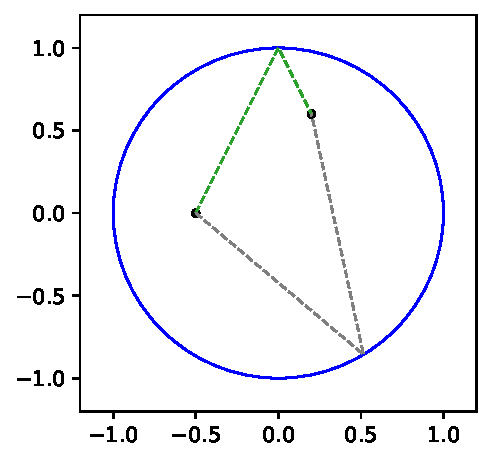
\includegraphics{ADOneDimManually_files/figure-pdf/fig-billardproblemsolutionwithmathsad-output-1.pdf}

}

\caption{\label{fig-billardproblemsolutionwithmathsad}Lösung des
Billardproblems mit anderen Startwerten.}

\end{figure}

\end{tcolorbox}

\begin{exercise}[Kürzeste Distanz mit
\texttt{mathsad}]\protect\hypertarget{exr-minDistSolutionWithSAD}{}\label{exr-minDistSolutionWithSAD}

Verwende das Modul \texttt{mathsad}, um die Lösung von
Übungsaufgabe~\ref{exr-MinDistlSolution} zu vereinfachen. Weil
\texttt{d} nun \texttt{FloatSad}-Objekte zurückgibt, muss auch die
Funktion \texttt{gradient\_descent(f,\ x0,\ lam)} angepasst werden.

\end{exercise}

\begin{tcolorbox}[enhanced jigsaw, titlerule=0mm, title=\textcolor{quarto-callout-tip-color}{\faLightbulb}\hspace{0.5em}{Lösung}, breakable, coltitle=black, leftrule=.75mm, bottomrule=.15mm, colback=white, rightrule=.15mm, opacitybacktitle=0.6, bottomtitle=1mm, toptitle=1mm, left=2mm, toprule=.15mm, colbacktitle=quarto-callout-tip-color!10!white, colframe=quarto-callout-tip-color-frame, arc=.35mm, opacityback=0]

In der Funktion \texttt{gradient\_descent(f,\ x0,\ lam)} muss lediglich
die Berechnung des neuen Näherungswertes angepasst werden. Statt des
Graphen wird hier nur das globale Minimum als Punkt ausgegeben.

\begin{Shaded}
\begin{Highlighting}[]
\ImportTok{from}\NormalTok{ floatsad }\ImportTok{import}\NormalTok{ FloatSad}
\ImportTok{import}\NormalTok{ math}
\ImportTok{import}\NormalTok{ mathsad}

\KeywordTok{def}\NormalTok{ d(t):}
\NormalTok{    t }\OperatorTok{=}\NormalTok{ FloatSad(t)}
\NormalTok{    Px }\OperatorTok{=} \DecValTok{2} \OperatorTok{*}\NormalTok{ mathsad.cos(t) }\OperatorTok{{-}} \DecValTok{1}    \CommentTok{\# x{-}Koordinate von P}
\NormalTok{    Py }\OperatorTok{=} \FloatTok{1.5} \OperatorTok{*}\NormalTok{ mathsad.sin(t)      }\CommentTok{\# y{-}Koordinate von P}
\NormalTok{    Pz }\OperatorTok{=} \DecValTok{0}                         \CommentTok{\# z{-}Koordinate von P}
\NormalTok{    Qx }\OperatorTok{=} \OperatorTok{{-}}\DecValTok{3} \OperatorTok{*}\NormalTok{ mathsad.sin(}\DecValTok{2}\OperatorTok{*}\NormalTok{t)     }\CommentTok{\# x{-}Koordinate von Q}
\NormalTok{    Qy }\OperatorTok{=} \DecValTok{2} \OperatorTok{*}\NormalTok{ mathsad.cos(}\DecValTok{2}\OperatorTok{*}\NormalTok{t) }\OperatorTok{+} \DecValTok{1}  \CommentTok{\# y{-}Koordinate von Q}
\NormalTok{    Qz }\OperatorTok{=} \DecValTok{2} \OperatorTok{*}\NormalTok{ mathsad.sin(}\DecValTok{2}\OperatorTok{*}\NormalTok{t) }\OperatorTok{+} \DecValTok{1}  \CommentTok{\# z{-}Koordinate von Q}
\NormalTok{    y }\OperatorTok{=}\NormalTok{ mathsad.sqrt((Px}\OperatorTok{{-}}\NormalTok{Qx)}\OperatorTok{**}\DecValTok{2} \OperatorTok{+}\NormalTok{ (Py}\OperatorTok{{-}}\NormalTok{Qy)}\OperatorTok{**}\DecValTok{2} \OperatorTok{+}\NormalTok{ (Pz}\OperatorTok{{-}}\NormalTok{Qz)}\OperatorTok{**}\DecValTok{2}\NormalTok{)}
    \ControlFlowTok{return}\NormalTok{ y}

\KeywordTok{def}\NormalTok{ gradient\_descent(f, x0, lam):}
\NormalTok{    tol }\OperatorTok{=} \FloatTok{1e{-}9}
    \CommentTok{\# Erster Schritt berechnen}
\NormalTok{    y0 }\OperatorTok{=}\NormalTok{ f(x0)}
\NormalTok{    x1 }\OperatorTok{=}\NormalTok{ x0 }\OperatorTok{{-}}\NormalTok{ lam }\OperatorTok{*}\NormalTok{ y0.derivative}
    \ControlFlowTok{while}\NormalTok{ math.fabs(x1}\OperatorTok{{-}}\NormalTok{x0) }\OperatorTok{\textgreater{}}\NormalTok{ tol:}
\NormalTok{        x0 }\OperatorTok{=}\NormalTok{ x1}
\NormalTok{        y0 }\OperatorTok{=}\NormalTok{ f(x0)}
\NormalTok{        x1 }\OperatorTok{=}\NormalTok{ x0 }\OperatorTok{{-}}\NormalTok{ lam }\OperatorTok{*}\NormalTok{ y0.derivative}
    \ControlFlowTok{return}\NormalTok{ x1}


\NormalTok{t0 }\OperatorTok{=} \DecValTok{3}
\NormalTok{tmin }\OperatorTok{=}\NormalTok{ gradient\_descent(d, t0, }\FloatTok{0.01}\NormalTok{)}
\NormalTok{dmin }\OperatorTok{=}\NormalTok{ d(tmin)}
\BuiltInTok{print}\NormalTok{(}\StringTok{"Minimum bei ("}\NormalTok{, tmin, dmin.value, }\StringTok{")"}\NormalTok{)}
\end{Highlighting}
\end{Shaded}

\begin{verbatim}
Minimum bei ( 4.712388977478413 1.5 )
\end{verbatim}

\end{tcolorbox}

\bookmarksetup{startatroot}

\hypertarget{sec-HigherDimFunctions}{%
\chapter{Funktionen mit mehreren In- und
Outputs}\label{sec-HigherDimFunctions}}

Wir wollen nun unsere Betrachtungen erweitern auf Funktionen, die zu
einem Eingabewert mehrere Ausgabewerte produzieren, d.h.
\(f : \mathbb{R}\rightarrow\mathbb{R}^m\) (Parameterkurven) oder aus
mehreren Eingabewerten einen Ausgabewert berechnen, d.h.
\(f : \mathbb{R}^n \rightarrow\mathbb{R}\) oder im allgemeinen Fall aus
\(n\) Eingabewerten \(m\) Ausgabewerte berechnen, d.h.
\(f : \mathbb{R}^n \rightarrow\mathbb{R}^m\).

\hypertarget{funktionen-mit-mehreren-ausgabewerten}{%
\section{Funktionen mit mehreren
Ausgabewerten}\label{funktionen-mit-mehreren-ausgabewerten}}

Eine vektorwertige Funktion \(f : \mathbb{R}\rightarrow\mathbb{R}^m\)
mit

\[
f(t) = \begin{pmatrix} y_1(t) \\ \vdots \\ y_m(t) \end{pmatrix}
\]

kann man sich als eine Kurve in einem \(m\)-dimensionalen Raum
vorstellen. Im Beispiel~\ref{exm-GDApplication} wird etwa die Bahn des
Punktes \(Q\) durch die Funktion

\[
f(t) = \left( \begin{align*} -3 &\sin(2t) \\ 2 &\cos(2t) + 1 \\ 2 &\sin(2t) + 1 \end{align*}  \right)
\]

beschrieben. Die Ableitung einer solchen Funktion wird komponentenweise
berechnet und gibt zu einem bestimmten Zeitpunkt \(t_0\) den
Tangentialvektor im Kurvenpunkt \(f(t_0)\) an:

\[
\dot{f}(t_0) = \begin{pmatrix} \dot y_1(t_0) \\ \vdots \\ \dot y_m(t_0) \end{pmatrix}
\]

Physikalisch entspricht dies dem Geschwindigkeitsvektor zum Zeitpunkt
\(t_0\). Mehr über die Ableitung von Parameterkurven findet man z.B. in
Arens u.~a. (2022), S. 947.

Als Programm können wir die obige Kurve so darstellen

\begin{Shaded}
\begin{Highlighting}[]
\ImportTok{import}\NormalTok{ math}

\KeywordTok{def}\NormalTok{ f(t):}
\NormalTok{    y1 }\OperatorTok{=} \OperatorTok{{-}}\DecValTok{3}\OperatorTok{*}\NormalTok{math.sin(}\DecValTok{2}\OperatorTok{*}\NormalTok{t)}
\NormalTok{    y2 }\OperatorTok{=}  \DecValTok{2}\OperatorTok{*}\NormalTok{math.cos(}\DecValTok{2}\OperatorTok{*}\NormalTok{t) }\OperatorTok{+} \DecValTok{1}
\NormalTok{    y3 }\OperatorTok{=}  \DecValTok{2}\OperatorTok{*}\NormalTok{math.sin(}\DecValTok{2}\OperatorTok{*}\NormalTok{t) }\OperatorTok{+} \DecValTok{1}
\NormalTok{    y }\OperatorTok{=}\NormalTok{ [y1, y2, y3]}
    \ControlFlowTok{return}\NormalTok{ y}

\NormalTok{t0 }\OperatorTok{=} \DecValTok{2}
\NormalTok{y0 }\OperatorTok{=}\NormalTok{ f(t0)}
\BuiltInTok{print}\NormalTok{(y0)}
\end{Highlighting}
\end{Shaded}

\begin{verbatim}
[2.2704074859237844, -0.3072872417272239, -0.5136049906158564]
\end{verbatim}

Für die Ableitung können wir unser Modul \texttt{FloatSad} benutzen. Der
Rückgabewert der Funktion ist dann eine Liste mit drei
\texttt{FloatSad}-Objekten.

\begin{Shaded}
\begin{Highlighting}[]
\ImportTok{from}\NormalTok{ floatsad }\ImportTok{import}\NormalTok{ FloatSad }
\ImportTok{import}\NormalTok{ mathsad}

\KeywordTok{def}\NormalTok{ f(t):}
\NormalTok{    t }\OperatorTok{=}\NormalTok{ FloatSad(t)}
\NormalTok{    y1 }\OperatorTok{=} \OperatorTok{{-}}\DecValTok{3}\OperatorTok{*}\NormalTok{mathsad.sin(}\DecValTok{2}\OperatorTok{*}\NormalTok{t)}
\NormalTok{    y2 }\OperatorTok{=}  \DecValTok{2}\OperatorTok{*}\NormalTok{mathsad.cos(}\DecValTok{2}\OperatorTok{*}\NormalTok{t) }\OperatorTok{+} \DecValTok{1}
\NormalTok{    y3 }\OperatorTok{=}  \DecValTok{2}\OperatorTok{*}\NormalTok{mathsad.sin(}\DecValTok{2}\OperatorTok{*}\NormalTok{t) }\OperatorTok{+} \DecValTok{1}
\NormalTok{    y }\OperatorTok{=}\NormalTok{ [y1, y2, y3]}
    \ControlFlowTok{return}\NormalTok{ y}

\NormalTok{t0 }\OperatorTok{=} \DecValTok{2}
\NormalTok{y0 }\OperatorTok{=}\NormalTok{ f(t0)}
\BuiltInTok{print}\NormalTok{(}\StringTok{"y1("} \OperatorTok{+} \BuiltInTok{str}\NormalTok{(t0) }\OperatorTok{+} \StringTok{") = "} \OperatorTok{+} \BuiltInTok{str}\NormalTok{(y0[}\DecValTok{0}\NormalTok{].value))}
\BuiltInTok{print}\NormalTok{(}\StringTok{"y1\textquotesingle{}("} \OperatorTok{+} \BuiltInTok{str}\NormalTok{(t0) }\OperatorTok{+} \StringTok{") = "} \OperatorTok{+} \BuiltInTok{str}\NormalTok{(y0[}\DecValTok{0}\NormalTok{].derivative))}
\end{Highlighting}
\end{Shaded}

\begin{verbatim}
y1(2) = 2.2704074859237844
y1'(2) = 3.921861725181672
\end{verbatim}

Diese Implementation hat den Nachteil, dass die Handhabung etwas
kompliziert wird. Insbesondere kann man nicht einfach \texttt{y0.value}
schreiben, um eine Liste der Funktionswerte zu erhalten. Abhilfe schafft
dabei das Modul \texttt{numpy}. Wir verwenden daraus die Möglichkeit,
Funktionen zu vektorisieren, um zwei Funktionen \texttt{getValues(y)}
und \texttt{getDerivatives(y)} zu definieren, welche aus der Liste
\texttt{y} von \texttt{FloatSad}-Objekten jeweils die Funktionswerte,
respektive die Werte der Ableitungen extrahieren.

\begin{Shaded}
\begin{Highlighting}[]
\ImportTok{from}\NormalTok{ floatsad }\ImportTok{import}\NormalTok{ FloatSad}
\ImportTok{import}\NormalTok{ mathsad}
\ImportTok{import}\NormalTok{ numpy }\ImportTok{as}\NormalTok{ np}

\KeywordTok{def}\NormalTok{ f(t):}
\NormalTok{    t }\OperatorTok{=}\NormalTok{ FloatSad(t)}
\NormalTok{    y1 }\OperatorTok{=} \OperatorTok{{-}}\DecValTok{3}\OperatorTok{*}\NormalTok{mathsad.sin(}\DecValTok{2}\OperatorTok{*}\NormalTok{t)}
\NormalTok{    y2 }\OperatorTok{=}  \DecValTok{2}\OperatorTok{*}\NormalTok{mathsad.cos(}\DecValTok{2}\OperatorTok{*}\NormalTok{t) }\OperatorTok{+} \DecValTok{1}
\NormalTok{    y3 }\OperatorTok{=}  \DecValTok{2}\OperatorTok{*}\NormalTok{mathsad.sin(}\DecValTok{2}\OperatorTok{*}\NormalTok{t) }\OperatorTok{+} \DecValTok{1}
\NormalTok{    y }\OperatorTok{=}\NormalTok{ [y1, y2, y3]}
    \ControlFlowTok{return}\NormalTok{ y}

\NormalTok{getValues }\OperatorTok{=}\NormalTok{ np.vectorize(}\KeywordTok{lambda}\NormalTok{ y : y.value)}
\NormalTok{getDerivatives }\OperatorTok{=}\NormalTok{ np.vectorize(}\KeywordTok{lambda}\NormalTok{ y : y.derivative)}

\NormalTok{t0 }\OperatorTok{=} \DecValTok{2}
\NormalTok{y0 }\OperatorTok{=}\NormalTok{ f(t0)}
\BuiltInTok{print}\NormalTok{(getValues(y0))}
\BuiltInTok{print}\NormalTok{(getDerivatives(y0))}
\end{Highlighting}
\end{Shaded}

\begin{verbatim}
[ 2.27040749 -0.30728724 -0.51360499]
[ 3.92186173  3.02720998 -2.61457448]
\end{verbatim}

\hypertarget{sec-FunktionenMehrereInputs}{%
\section{Funktionen mit mehreren
Eingabewerten}\label{sec-FunktionenMehrereInputs}}

Die Ableitung einer Funktion \(f : \mathbb{R}^n \rightarrow \mathbb{R}\)
ist der Gradient

\[
\nabla f = \left( \frac{\partial f}{\partial x_1}, \ldots, \frac{\partial f}{\partial x_n} \right)
\]

Für weitere Details zum Gradienten sei auf Arens u.~a. (2022), S. 870
verwiesen.

\begin{example}[Eine Funktion mit drei
Eingabwerten]\protect\hypertarget{exm-ExampleFunctionRnToR}{}\label{exm-ExampleFunctionRnToR}

Betrachten wir als Beispiel die Funktion
\(f : \mathbb{R}^3 \rightarrow \mathbb{R}\)

\[
f(x_0, x_1, x_2) = x_0^2 + 2\cdot x_0 \cdot x_1 - \frac{x_1}{x_2 ^3}
\]

Das folgende Programm berechnet den Funktionswert
\(f(1, 2, 3)=\frac{133}{27}\approx 4.9259...\)

\begin{Shaded}
\begin{Highlighting}[]
\KeywordTok{def}\NormalTok{ f(x):}
\NormalTok{    y }\OperatorTok{=}\NormalTok{ x[}\DecValTok{0}\NormalTok{]}\OperatorTok{**}\DecValTok{2} \OperatorTok{+} \DecValTok{2}\OperatorTok{*}\NormalTok{x[}\DecValTok{0}\NormalTok{]}\OperatorTok{*}\NormalTok{x[}\DecValTok{1}\NormalTok{] }\OperatorTok{{-}}\NormalTok{ x[}\DecValTok{1}\NormalTok{]}\OperatorTok{/}\NormalTok{x[}\DecValTok{2}\NormalTok{]}\OperatorTok{**}\DecValTok{3}
    \ControlFlowTok{return}\NormalTok{ y}

\NormalTok{x0 }\OperatorTok{=}\NormalTok{ [}\DecValTok{1}\NormalTok{, }\DecValTok{2}\NormalTok{, }\DecValTok{3}\NormalTok{]}
\NormalTok{y0 }\OperatorTok{=}\NormalTok{ f(x0)}
\BuiltInTok{print}\NormalTok{(y0)}
\end{Highlighting}
\end{Shaded}

\begin{verbatim}
4.925925925925926
\end{verbatim}

Der Gradient dieser Funktion ist \[
\nabla f = \left( 2x_0+2x_1, 2x_0 - \frac{1}{x_2^3}, 3\frac{x_1}{x_2^4} \right)
\]

bzw. ausgewertet an der Stelle \((x_0, x_1, x_2) = (1, 2, 3)\) \[
\begin{align*}
\nabla f \vert _{(1, 2, 3)} &= \left( 6, \frac{53}{27}, \frac2{27} \right) \\
&\approx \left( 6, 1.9629..., 0.0740... \right)
\end{align*}
\]

\end{example}

\begin{center}\rule{0.5\linewidth}{0.5pt}\end{center}

Mit der Standard Algorithmischen Differentiation kann der Gradient nicht
in einem Durchgang berechnet werden. Bei der Umwandlung der Anfangswerte
in \texttt{FloatSad}-Objekte müssen wir allen Variablen in
\(x = (x_1, \ldots, x_n)\) einen Anfangswert
\(\dot{x} = (\dot x_1, \ldots, \dot x_n)\) geben. Wenn wir für die
Initialisierung \(\dot{x} = e_i = (0, \ldots, 1, \ldots, 0)\) verwenden
(mit \(1\) an der \(i\)-ten Stelle und sonst lauter \(0\)), dann
bekommen wir den Wert der \(i\)-ten partiellen Ableitung
\(\frac{\partial f}{\partial x_i}\).

Um die Funktion im obigen Beispiel mit unserer Klasse \texttt{FloatSad}
abzuleiten, verwenden wir wieder \texttt{numpy}. Als erstes definieren
wir eine vektorisierte Funktion \texttt{float2FloatSad}, mit der wir aus
der Liste \texttt{x} eine Liste von \texttt{FloatSad}-Objekten erzeugen.
Die Werte der Ableitungen werden zu Beginn explizit in der Variablen
\texttt{xdot} initialisiert.

\section{\texorpdfstring{Ableitung nach \texttt{x0}}{Ableitung nach x0}}

\begin{Shaded}
\begin{Highlighting}[]
\ImportTok{from}\NormalTok{ floatsad }\ImportTok{import}\NormalTok{ FloatSad}
\ImportTok{import}\NormalTok{ numpy }\ImportTok{as}\NormalTok{ np}

\KeywordTok{def}\NormalTok{ f(x):}
\NormalTok{    xdot }\OperatorTok{=}\NormalTok{ [}\DecValTok{1}\NormalTok{, }\DecValTok{0}\NormalTok{, }\DecValTok{0}\NormalTok{]}
\NormalTok{    x }\OperatorTok{=}\NormalTok{ float2FloatSad(x, xdot)}
\NormalTok{    y }\OperatorTok{=}\NormalTok{ x[}\DecValTok{0}\NormalTok{]}\OperatorTok{**}\DecValTok{2} \OperatorTok{+} \DecValTok{2}\OperatorTok{*}\NormalTok{x[}\DecValTok{0}\NormalTok{]}\OperatorTok{*}\NormalTok{x[}\DecValTok{1}\NormalTok{] }\OperatorTok{{-}}\NormalTok{ x[}\DecValTok{1}\NormalTok{]}\OperatorTok{/}\NormalTok{x[}\DecValTok{2}\NormalTok{]}\OperatorTok{**}\DecValTok{3}
    \ControlFlowTok{return}\NormalTok{ y}

\NormalTok{float2FloatSad }\OperatorTok{=}\NormalTok{ np.vectorize(}\KeywordTok{lambda}\NormalTok{ x, v : FloatSad(x,v))}

\NormalTok{x0 }\OperatorTok{=}\NormalTok{ [}\DecValTok{1}\NormalTok{, }\DecValTok{2}\NormalTok{, }\DecValTok{3}\NormalTok{]}
\NormalTok{y0 }\OperatorTok{=}\NormalTok{ f(x0)}
\BuiltInTok{print}\NormalTok{(y0)}
\end{Highlighting}
\end{Shaded}

\begin{verbatim}
< 4.925925925925926 ; 6.0 >
\end{verbatim}

\section{\texorpdfstring{Ableitung nach \texttt{x1}}{Ableitung nach x1}}

\begin{Shaded}
\begin{Highlighting}[]
\ImportTok{from}\NormalTok{ floatsad }\ImportTok{import}\NormalTok{ FloatSad}
\ImportTok{import}\NormalTok{ numpy }\ImportTok{as}\NormalTok{ np}

\KeywordTok{def}\NormalTok{ f(x):}
\NormalTok{    xdot }\OperatorTok{=}\NormalTok{ [}\DecValTok{0}\NormalTok{, }\DecValTok{1}\NormalTok{, }\DecValTok{0}\NormalTok{]}
\NormalTok{    x }\OperatorTok{=}\NormalTok{ float2FloatSad(x, xdot)}
\NormalTok{    y }\OperatorTok{=}\NormalTok{ x[}\DecValTok{0}\NormalTok{]}\OperatorTok{**}\DecValTok{2} \OperatorTok{+} \DecValTok{2}\OperatorTok{*}\NormalTok{x[}\DecValTok{0}\NormalTok{]}\OperatorTok{*}\NormalTok{x[}\DecValTok{1}\NormalTok{] }\OperatorTok{{-}}\NormalTok{ x[}\DecValTok{1}\NormalTok{]}\OperatorTok{/}\NormalTok{x[}\DecValTok{2}\NormalTok{]}\OperatorTok{**}\DecValTok{3}
    \ControlFlowTok{return}\NormalTok{ y}

\NormalTok{float2FloatSad }\OperatorTok{=}\NormalTok{ np.vectorize(}\KeywordTok{lambda}\NormalTok{ x, v : FloatSad(x,v))}

\NormalTok{x0 }\OperatorTok{=}\NormalTok{ [}\DecValTok{1}\NormalTok{, }\DecValTok{2}\NormalTok{, }\DecValTok{3}\NormalTok{]}
\NormalTok{y0 }\OperatorTok{=}\NormalTok{ f(x0)}
\BuiltInTok{print}\NormalTok{(y0)}
\end{Highlighting}
\end{Shaded}

\begin{verbatim}
< 4.925925925925926 ; 1.962962962962963 >
\end{verbatim}

\section{\texorpdfstring{Ableitung nach \texttt{x2}}{Ableitung nach x2}}

\begin{Shaded}
\begin{Highlighting}[]
\ImportTok{from}\NormalTok{ floatsad }\ImportTok{import}\NormalTok{ FloatSad}
\ImportTok{import}\NormalTok{ numpy }\ImportTok{as}\NormalTok{ np}

\KeywordTok{def}\NormalTok{ f(x):}
\NormalTok{    xdot }\OperatorTok{=}\NormalTok{ [}\DecValTok{0}\NormalTok{, }\DecValTok{0}\NormalTok{, }\DecValTok{1}\NormalTok{]}
\NormalTok{    x }\OperatorTok{=}\NormalTok{ float2FloatSad(x, xdot)}
\NormalTok{    y }\OperatorTok{=}\NormalTok{ x[}\DecValTok{0}\NormalTok{]}\OperatorTok{**}\DecValTok{2} \OperatorTok{+} \DecValTok{2}\OperatorTok{*}\NormalTok{x[}\DecValTok{0}\NormalTok{]}\OperatorTok{*}\NormalTok{x[}\DecValTok{1}\NormalTok{] }\OperatorTok{{-}}\NormalTok{ x[}\DecValTok{1}\NormalTok{]}\OperatorTok{/}\NormalTok{x[}\DecValTok{2}\NormalTok{]}\OperatorTok{**}\DecValTok{3}
    \ControlFlowTok{return}\NormalTok{ y}

\NormalTok{float2FloatSad }\OperatorTok{=}\NormalTok{ np.vectorize(}\KeywordTok{lambda}\NormalTok{ x, v : FloatSad(x,v))}

\NormalTok{x0 }\OperatorTok{=}\NormalTok{ [}\DecValTok{1}\NormalTok{, }\DecValTok{2}\NormalTok{, }\DecValTok{3}\NormalTok{]}
\NormalTok{y0 }\OperatorTok{=}\NormalTok{ f(x0)}
\BuiltInTok{print}\NormalTok{(y0)}
\end{Highlighting}
\end{Shaded}

\begin{verbatim}
< 4.925925925925926 ; 0.07407407407407407 >
\end{verbatim}

Initialisiert man die Ableitungen beispielsweise mit
\texttt{xdot\ =\ {[}1,\ 1,\ 1{]}}, dann erhält man die Summe der drei
Richtungsableitungen:

\begin{verbatim}
< 4.925925925925926 ; 8.037037037037036 >
\end{verbatim}

Allgemein gilt: Initialisiert man \texttt{xdot} mit dem Vektor
\(\vec r = (r_1, \ldots, r_n)^\intercal\), dann erhält man das
Skalarprodukt \[
\nabla f \cdot \vec r = 
\left ( \left .\frac{\partial f}{\partial x_1} \right \vert_{(x_1, \ldots, x_n)}, \ldots, \left .\frac{\partial f}{\partial x_n} \right \vert_{(x_1, \ldots, x_n)}  \right ) \cdot \begin{pmatrix} r_1 \\ \vdots \\ r_n \end{pmatrix} 
\]

\hypertarget{sec-FuncRnToRm}{%
\section{Funktionen mit mehreren Ein- und
Ausgabewerten}\label{sec-FuncRnToRm}}

Eine Funktion \(f : \mathbb{R}^n \rightarrow \mathbb{R}^m\) hat die Form
\[
f(x_1, \ldots, x_n) = \left( \begin{align*} y_1(x_1, &\ldots, x_n) \\ &\vdots \\ y_m(x_1, &\ldots, x_n) \end{align*} \right)
\] Die Ableitung einer solchen Funktion wird durch die Jacobi Matrix \[
Jf = \begin{pmatrix}
    \frac{\partial y_1}{\partial x_1} & \ldots & \frac{\partial y_1}{\partial x_n} \\
    \vdots & & \vdots \\
    \frac{\partial y_m}{\partial x_1} & \ldots & \frac{\partial y_m}{\partial x_n}
\end{pmatrix}
\in\mathbb{R}^{m\times n}
\] gegeben. Auch hierzu findet der Leser mehr Informationen in Arens
u.~a. (2022), S. 878.

\begin{example}[Eine Funktion mit zwei Ein- und drei
Ausgabwerten]\protect\hypertarget{exm-ExFunctionR2ToR3}{}\label{exm-ExFunctionR2ToR3}

Betrachte die Funktion \(f : \mathbb{R}^2 \rightarrow \mathbb{R}^3\) \[
f(x_0, x_1) = 
    \begin{pmatrix}
        x_0\cdot \sqrt{x_1} + 3x_1 \\
        \cos(x_0) / x_1 \\
        e^{x_0 ^2\cdot x_1}
    \end{pmatrix}
\]

Die Jacobi Matrix lautet in diesem Fall \[
Jf = 
\begin{pmatrix}
    \sqrt{x_1} & \frac{x_0}{2\sqrt{x_1}} + 3 \\
    -\frac{\sin(x_0)}{x_1} & -\frac{\cos(x_0)}{x_1^2} \\
    e^{x_0^2\cdot x_1}\cdot 2 x_0 x_1 & e^{x_0^2\cdot x_1}\cdot x_0^2
\end{pmatrix}
\]

Ausgewertet an der Stelle \((x_0, x_1) = (2, 1)\) ergibt dies
\begin{align*}
f(2,1) &\approx \begin{pmatrix} 5 \\ -0.4161... \\ 54.5981... \end{pmatrix}, \\ 
JF \vert _{(2,1)} &\approx 
    \begin{pmatrix}  
        1 & 4 \\
        -0.9092... & 0.4161... \\
        218.3926... & 218.3926...
    \end{pmatrix}
\end{align*}

\end{example}

\begin{center}\rule{0.5\linewidth}{0.5pt}\end{center}

Um die Funktion aus dem Beispiel mit SAD abzuleiten kombinieren wir die
Techniken aus den beiden vorherigen Abschnitten. Je nach Initialisierung
von \texttt{xdot} erhalten wir die erste oder die zweite Spalte von
\(JF\).

\section{1. Spalte}

\begin{Shaded}
\begin{Highlighting}[]
\ImportTok{from}\NormalTok{ floatsad }\ImportTok{import}\NormalTok{ FloatSad}
\ImportTok{import}\NormalTok{ mathsad}
\ImportTok{import}\NormalTok{ numpy }\ImportTok{as}\NormalTok{ np}

\KeywordTok{def}\NormalTok{ f(x):}
\NormalTok{    xdot }\OperatorTok{=}\NormalTok{ [}\DecValTok{1}\NormalTok{, }\DecValTok{0}\NormalTok{]}
\NormalTok{    x }\OperatorTok{=}\NormalTok{ float2FloatSad(x, xdot)}
\NormalTok{    y1 }\OperatorTok{=}\NormalTok{ x[}\DecValTok{0}\NormalTok{]}\OperatorTok{*}\NormalTok{mathsad.sqrt(x[}\DecValTok{1}\NormalTok{]) }\OperatorTok{+} \DecValTok{3}\OperatorTok{*}\NormalTok{x[}\DecValTok{1}\NormalTok{]}
\NormalTok{    y2 }\OperatorTok{=}\NormalTok{ mathsad.cos(x[}\DecValTok{0}\NormalTok{]) }\OperatorTok{/}\NormalTok{ x[}\DecValTok{1}\NormalTok{]}
\NormalTok{    y3 }\OperatorTok{=}\NormalTok{ mathsad.exp(x[}\DecValTok{0}\NormalTok{]}\OperatorTok{**}\DecValTok{2} \OperatorTok{*}\NormalTok{ x[}\DecValTok{1}\NormalTok{])}
    \ControlFlowTok{return}\NormalTok{ [y1, y2, y3]    }


\NormalTok{float2FloatSad }\OperatorTok{=}\NormalTok{ np.vectorize(}\KeywordTok{lambda}\NormalTok{ x, v : FloatSad(x,v))}
\NormalTok{getValues }\OperatorTok{=}\NormalTok{ np.vectorize(}\KeywordTok{lambda}\NormalTok{ y : y.value)}
\NormalTok{getDerivatives }\OperatorTok{=}\NormalTok{ np.vectorize(}\KeywordTok{lambda}\NormalTok{ y : y.derivative)}


\NormalTok{x0 }\OperatorTok{=}\NormalTok{ (}\DecValTok{2}\NormalTok{, }\DecValTok{1}\NormalTok{)}
\NormalTok{y0 }\OperatorTok{=}\NormalTok{ f(x0)}
\BuiltInTok{print}\NormalTok{(}\StringTok{"Funktionswerte:"}\NormalTok{)}
\BuiltInTok{print}\NormalTok{(getValues(y0))}
\BuiltInTok{print}\NormalTok{(}\StringTok{"1. Spalte von Jf:"}\NormalTok{)}
\BuiltInTok{print}\NormalTok{(getDerivatives(y0))}
\end{Highlighting}
\end{Shaded}

\begin{verbatim}
Funktionswerte:
[ 5.         -0.41614684 54.59815003]
1. Spalte von Jf:
[  1.          -0.90929743 218.39260013]
\end{verbatim}

\section{2. Spalte}

\begin{Shaded}
\begin{Highlighting}[]
\ImportTok{from}\NormalTok{ floatsad }\ImportTok{import}\NormalTok{ FloatSad}
\ImportTok{import}\NormalTok{ mathsad}
\ImportTok{import}\NormalTok{ numpy }\ImportTok{as}\NormalTok{ np}

\KeywordTok{def}\NormalTok{ f(x):}
\NormalTok{    xdot }\OperatorTok{=}\NormalTok{ [}\DecValTok{0}\NormalTok{, }\DecValTok{1}\NormalTok{]}
\NormalTok{    x }\OperatorTok{=}\NormalTok{ float2FloatSad(x, xdot)}
\NormalTok{    y1 }\OperatorTok{=}\NormalTok{ x[}\DecValTok{0}\NormalTok{]}\OperatorTok{*}\NormalTok{mathsad.sqrt(x[}\DecValTok{1}\NormalTok{]) }\OperatorTok{+} \DecValTok{3}\OperatorTok{*}\NormalTok{x[}\DecValTok{1}\NormalTok{]}
\NormalTok{    y2 }\OperatorTok{=}\NormalTok{ mathsad.cos(x[}\DecValTok{0}\NormalTok{]) }\OperatorTok{/}\NormalTok{ x[}\DecValTok{1}\NormalTok{]}
\NormalTok{    y3 }\OperatorTok{=}\NormalTok{ mathsad.exp(x[}\DecValTok{0}\NormalTok{]}\OperatorTok{**}\DecValTok{2} \OperatorTok{*}\NormalTok{ x[}\DecValTok{1}\NormalTok{])}
    \ControlFlowTok{return}\NormalTok{ [y1, y2, y3]    }


\NormalTok{float2FloatSad }\OperatorTok{=}\NormalTok{ np.vectorize(}\KeywordTok{lambda}\NormalTok{ x, v : FloatSad(x,v))}
\NormalTok{getValues }\OperatorTok{=}\NormalTok{ np.vectorize(}\KeywordTok{lambda}\NormalTok{ y : y.value)}
\NormalTok{getDerivatives }\OperatorTok{=}\NormalTok{ np.vectorize(}\KeywordTok{lambda}\NormalTok{ y : y.derivative)}


\NormalTok{x0 }\OperatorTok{=}\NormalTok{ (}\DecValTok{2}\NormalTok{, }\DecValTok{1}\NormalTok{)}
\NormalTok{y0 }\OperatorTok{=}\NormalTok{ f(x0)}
\BuiltInTok{print}\NormalTok{(}\StringTok{"Funktionswerte:"}\NormalTok{)}
\BuiltInTok{print}\NormalTok{(getValues(y0))}
\BuiltInTok{print}\NormalTok{(}\StringTok{"2. Spalte von Jf:"}\NormalTok{)}
\BuiltInTok{print}\NormalTok{(getDerivatives(y0))}
\end{Highlighting}
\end{Shaded}

\begin{verbatim}
Funktionswerte:
[ 5.         -0.41614684 54.59815003]
2. Spalte von Jf:
[  4.           0.41614684 218.39260013]
\end{verbatim}

Initialisiert man allgemein \texttt{xdot} mit dem Vektor
\(\vec{r} = (r_1, \ldots, r_n)^\intercal\), dann erhält man als Resultat
das Produkt \[
Jf \cdot \vec{r} = 
\begin{pmatrix}
    \frac{\partial y_1}{\partial x_1} & \ldots & \frac{\partial y_1}{\partial x_n} \\
    \vdots & & \vdots \\
    \frac{\partial y_m}{\partial x_1} & \ldots & \frac{\partial y_m}{\partial x_n}
\end{pmatrix}
\cdot \begin{pmatrix} r_1 \\ \vdots \\ r_n \end{pmatrix} 
\]

Braucht man die gesammte Jacobi Matrix, dann muss man also die Funktion
so oft aufrufen, wie die Matrix Spalten hat, d.h. \texttt{len(x)} Mal.
Die SAD Methode ist also effizient, wenn eine Funktion mehr Aus- als
Eingabewerte hat. Der ineffizienteste Fall tritt auf, wenn die Funktion
aus vielen Eingabewerte nur einen Ausgabewert berechnet. Mit anderen
Worten: Das Bestimmen des Gradienten einer Funktion
\(f: \mathbb{R}^n \rightarrow \mathbb{R}\) benötigt den grössten Aufwand
gemessen an der Anzahl der zu berechnenden Werte. Abhilfe schafft in so
einem Fall die Adjungierte Automatische Differentiation (AAD).

Zum Schluss sei noch angemerkt, dass die Definition der drei Funktionen
\texttt{float2FloatSad}, \texttt{getValues} und \texttt{getDerivatives}
in die Datei \texttt{floatsad.py} geschrieben werden könnten (beachte,
dass sie \emph{nicht} eingerückt werden wie die restlichen Befehle der
Klasse). Dann vereinfacht sich das obige Programm:

\begin{Shaded}
\begin{Highlighting}[]
\ImportTok{from}\NormalTok{ floatsad }\ImportTok{import} \OperatorTok{*}
\ImportTok{import}\NormalTok{ mathsad}

\KeywordTok{def}\NormalTok{ f(x):}
\NormalTok{    xdot }\OperatorTok{=}\NormalTok{ [}\DecValTok{1}\NormalTok{, }\DecValTok{0}\NormalTok{]}
\NormalTok{    x }\OperatorTok{=}\NormalTok{ float2FloatSad(x, xdot)}
\NormalTok{    y1 }\OperatorTok{=}\NormalTok{ x[}\DecValTok{0}\NormalTok{]}\OperatorTok{*}\NormalTok{mathsad.sqrt(x[}\DecValTok{1}\NormalTok{]) }\OperatorTok{+} \DecValTok{3}\OperatorTok{*}\NormalTok{x[}\DecValTok{1}\NormalTok{]}
\NormalTok{    y2 }\OperatorTok{=}\NormalTok{ mathsad.cos(x[}\DecValTok{0}\NormalTok{]) }\OperatorTok{/}\NormalTok{ x[}\DecValTok{1}\NormalTok{]}
\NormalTok{    y3 }\OperatorTok{=}\NormalTok{ mathsad.exp(x[}\DecValTok{0}\NormalTok{]}\OperatorTok{**}\DecValTok{2} \OperatorTok{*}\NormalTok{ x[}\DecValTok{1}\NormalTok{])}
    \ControlFlowTok{return}\NormalTok{ [y1, y2, y3]    }

\NormalTok{x0 }\OperatorTok{=}\NormalTok{ (}\DecValTok{2}\NormalTok{, }\DecValTok{1}\NormalTok{)}
\NormalTok{y0 }\OperatorTok{=}\NormalTok{ f(x0)}
\BuiltInTok{print}\NormalTok{(getValues(y0))}
\BuiltInTok{print}\NormalTok{(getDerivatives(y0))}
\end{Highlighting}
\end{Shaded}

\bookmarksetup{startatroot}

\hypertarget{sec-AAD}{%
\chapter{Adjungierte Algorithmische Differentiation}\label{sec-AAD}}

In Kapitel~\ref{sec-HigherDimFunctions} haben wir gesehen, dass wir mit
der Standard Algorithmischen Differentiation (SAD) alle \(m\)
Ableitungen einer Funktion \(f : \mathbb{R} \rightarrow \mathbb{R}^m\)
mit einem einzigen Funktionsaufruf berechnen können. Die Berechnung des
Gradienten einer Funktion \(f : \mathbb{R}^n \rightarrow \mathbb{R}\)
benötigt jedoch \(n\) Funktionsaufrufe, nämlich einen für jede partielle
Ableitung \(\partial f / \partial x_i\). In diesem Kapitel wollen wir
eine Methode entwickeln, die alle \(n\) partiellen Ableitungen in einem
Funktionsaufruf berechnet.

Ähnlich wie die SAD beruht auch diese Methode darauf, dass wir eine
komplizierte Funktion schrittweise mit Hilfe von elementaren Operationen
berechnen und in jedem Schritt die Ableitungen in separaten Variablen
akkumulieren. Wir führen also wieder unsere Konvention aus
Kapitel~\ref{sec-ProgFunc} ein. Auch dieses Mal werden wir in jedem
Schritt die Kettenregel verwenden. Diesmal fangen wir jedoch am Ende der
Funktion an und werden uns dann rückwärts durch alle Ableitungen
arbeiten. Aus diesem Grund wird das Verfahren auch Rückwärts-AD
\footnote{Im Englischen spricht man von \emph{reverse mode
  differentiation} weil \emph{backward differentiation} für bestimmte
  Methoden zur Integration von Differentialgleichungen verwendet wird.}
oder Adjungierte AD (AAD) genannt.

\hypertarget{manuelle-implementation-der-aad}{%
\section{Manuelle Implementation der
AAD}\label{manuelle-implementation-der-aad}}

Wir erläutern die Methode zuerst an einem einfachen Beispiel, welches
eine leicht abgeänderte Version des Beispiels von Radcliffe (2021) ist.

\begin{example}[Gradient mit
AAD]\protect\hypertarget{exm-firstAADbyHand}{}\label{exm-firstAADbyHand}

Betrachten wir die Funktion \(f : \mathbb{R}^2 \rightarrow \mathbb{R}\)
\[
y = f(x_0, x_1) = (x_0 + x_1) \cdot x_0 - x_1
\]

Als Programm können wir die Funktion unter Berücksichtigung der
Konvention so schreiben (siehe auch Abbildung~\ref{fig-compTreeMulti}):

\begin{Shaded}
\begin{Highlighting}[]
\KeywordTok{def}\NormalTok{ f(x0, x1):}
\NormalTok{    v0 }\OperatorTok{=}\NormalTok{ x0}
\NormalTok{    v1 }\OperatorTok{=}\NormalTok{ x1}
\NormalTok{    v2 }\OperatorTok{=}\NormalTok{ v0 }\OperatorTok{+}\NormalTok{ v1}
\NormalTok{    v3 }\OperatorTok{=}\NormalTok{ v2 }\OperatorTok{*}\NormalTok{ v0}
\NormalTok{    v4 }\OperatorTok{=}\NormalTok{ v3 }\OperatorTok{{-}}\NormalTok{ v1}
\NormalTok{    y }\OperatorTok{=}\NormalTok{ v4}
    \ControlFlowTok{return}\NormalTok{ y}

\NormalTok{x0, x1 }\OperatorTok{=} \DecValTok{2}\NormalTok{, }\DecValTok{3}
\NormalTok{y0 }\OperatorTok{=}\NormalTok{ f(x0, x1)}
\BuiltInTok{print}\NormalTok{(}\StringTok{"f("} \OperatorTok{+} \BuiltInTok{str}\NormalTok{(x0) }\OperatorTok{+} \StringTok{","} \OperatorTok{+} \BuiltInTok{str}\NormalTok{(x1) }\OperatorTok{+} \StringTok{") = "} \OperatorTok{+} \BuiltInTok{str}\NormalTok{(y0))}
\end{Highlighting}
\end{Shaded}

\begin{verbatim}
f(2,3) = 7
\end{verbatim}

\begin{figure}

{\centering 

\begin{figure}[H]

{\centering \includegraphics[width=5.5in,height=3.5in]{aad_files/figure-latex/dot-figure-1.png}

}

\end{figure}

}

\caption{\label{fig-compTreeMulti}Computational Graph für
\texttt{y\ =\ (x0\ +\ x1)\ *\ x0\ -\ x1}.}

\end{figure}

Die partiellen Ableitungen von \(f\) lauten \[
\begin{align*}
    \frac{\partial y}{\partial x_0} &= \frac{\partial f}{\partial x_0} = (1+0)\cdot x_0 + (x_0 + x_1)\cdot 1 - 0=2x_0 + x_1 \\
    \frac{\partial y}{\partial x_1} &= \frac{\partial f}{\partial x_1} = (0 + 1)\cdot x_0 - 1 = x_0 - 1
\end{align*}
\] wobei für die Ableitung nach \(x_0\) die Produktregel verwendet
wurde. Die partielle Ableitung \(\partial y / \partial x_0\) können wir
auch berechnen, indem wir bei \(y = v_4\) anfangen und jeweils die
Definition der Hilfsvariablen einsetzen: \[
\begin{align*}
    \frac{\partial y}{\partial x_0} &= \frac{\partial v_4}{\partial x_0} \\
    &= \frac{\partial (v_3 - v_1)}{\partial x_0} \\
    &= \frac{\partial v_3}{\partial x_0} - \frac{\partial v_1}{\partial x_0} \\
    &= \frac{\partial (v_2 \cdot v_0)}{\partial x_0} - \frac{\partial x_1}{\partial x_0} \\
    &= \frac{\partial v_2}{\partial x_0} \cdot v_0 + v_2 \cdot \frac{\partial v_0}{\partial x_0} - 0 \\
    &= \frac{\partial (v_0 + v_1)}{\partial x_0} \cdot v_0 + v_2 \cdot \frac{\partial x_0}{\partial x_0} \\
    &= \left( \frac{\partial v_0}{\partial x_0} + \frac{\partial v_1}{\partial x_0} \right) \cdot x_0 + (v_0 + v_1) \cdot 1 \\
    &= \left( \frac{\partial x_0}{\partial x_0} + \frac{\partial x_1}{\partial x_0} \right) \cdot x_0 + (x_0 + x_1) \\
    &= (1 + 0) \cdot x_0 + (x_0 + x_1) \\
    &= 2x_0 + x_1   
\end{align*}
\]

Analog findet man \(\partial y / \partial x_1\) (diesmal lassen wir
einige der offensichtlicheren Zwischenschritte weg): \[
\begin{align*}
    \frac{\partial y}{\partial x_1} &= \frac{\partial v_4}{\partial x_1} \\
    &= \frac{\partial v_3}{\partial x_1} - \frac{\partial v_1}{\partial x_1} \\
    &= \frac{\partial (v_2 \cdot v_0)}{\partial x_1} - 1 \\
    &= \frac{\partial v_2}{\partial x_1} \cdot v_0 + v_2 \cdot \frac{\partial v_0}{\partial x_1} - 1 \\
    &= \frac{\partial (v_0 + v_1)}{\partial x_1} \cdot x_0 + v_2 \cdot 0 - 1 \\
    &= \left( \frac{\partial v_0}{\partial x_1} + \frac{\partial v_1}{\partial x_1} \right) \cdot x_0 - 1 \\
    &= ( 0 + 1) \cdot x_0 - 1 \\
    &= x_0 - 1   
\end{align*}
\]

Um die beiden Rechnungen zusammenzufassen, führen wir nun für jede
Hilfsvariable \(v_i\) eine neue Variable \(\bar v_i\) ein, welche
definiert ist als \[
\bar v_i = \frac{\partial y}{\partial v_i}
\] Ähnlich wie die \(\dot v_i\) aus der SAD speichern diese Variablen
die Werte der Ableitungen. Die neue Notation soll anzeigen, dass es sich
um die AAD Methode handelt. Unser Ziel ist es also,
\(\bar v_0 = \partial y / \partial v_0 = \partial y / \partial x_0\) und
\(\bar v_1 = \partial y / \partial v_1 = \partial y / \partial x_1\) zu
bestimmen. Beginnen wir in der letzten Zeile des Programms, dann gilt
offenbar immer \(\bar v_4 = \partial y / \partial v_4 = 1\). In der
Zeile darüber können wir \(\bar v_3\) und \(\bar v_1\) berechnen, indem
wir die Kettenregel verwenden.

\begin{align*}
    \bar v_3 &= \frac{\partial y}{\partial v_3} = \frac{\partial y}{\partial v_4} \cdot \frac{\partial v_4}{\partial v_3} = \bar v_4 \cdot (1-0)=\bar v_4  \\

    \bar v_1 &= \frac{\partial y}{\partial v_1} = \frac{\partial y}{\partial v_4} \cdot \frac{\partial v_4}{\partial v_1} = \bar v_4 \cdot (0-1)= -\bar v_4
\end{align*}

Also sind \(\bar v_3 = 1\) und \(\bar v_1 = -1\). Der Zwischenwert in
\(\bar v_1\) wird später ergänzt werden. Aus der Zeile
\(v_3 = v_2 \cdot v_0\) lassen sich als nächstes Ausdrücke für
\(\bar v_2\) und \(\bar v_0\) finden.

\begin{align*}
    \bar v_2 &= \frac{\partial y}{\partial v_2} = \frac{\partial y}{\partial v_3} \cdot \frac{\partial v_3}{\partial v_2} = \bar v_3 \cdot v_0 \\

    \bar v_0 &= \frac{\partial y}{\partial v_0} = \frac{\partial y}{\partial v_3} \cdot \frac{\partial v_3}{\partial v_0} = \bar v_3 \cdot v_2 
\end{align*}

Mit den vorher berechneten Werten erhalten wir also \(\bar v_2 = v_0\)
und \(\bar v_0 = v_2\). Beide Werte sind durch die Funktion bereits
berechnet worden. Im obigen Beispiel gilt etwa \texttt{v0\ =\ x0\ =\ 2}
und \texttt{v2\ =\ x0\ +\ x1\ =\ 5}. Auch diese Zwischenwerte werden im
nächsten Schritt ergänzt. Aus der Zeile \(v_2 = v_0 + v_1\) ergibt sich
nämlich

\begin{align*}
    \bar v_0 &= \bar v_0 + \frac{\partial y}{\partial v_0} = \bar v_0 + \frac{\partial y}{\partial v_2} \cdot \frac{\partial v_2}{\partial v_0} \\
    &= \bar v_0 + \bar v_2 \cdot (1+0) = \bar v_0 + \bar v_2 \\ & \\

    \bar v_1 &= \bar v_1 + \frac{\partial y}{\partial v_1} = \bar v_1 + \frac{\partial y}{\partial v_2} \cdot \frac{\partial v_2}{\partial v_1} \\
    &= \bar v_1 + \bar v_2 \cdot (0+1) = \bar v_1 + \bar v_2
\end{align*}

Mit den bereits bekannten Werten erhalten wir \(\bar v_0 = v_2 + v_0\)
(bzw. mit den konkreten Werten des Beispiels \texttt{v0bar\ =\ 5\ +\ 2})
und \(\bar v_1 = -1 + v_0\) (bzw. \texttt{v1bar\ =\ -1\ +\ 2}). Nun
enthalten die Variablen \(\bar v_0\) und \(\bar v_1\) die Werte der
gewünschten Ableitungen, nämlich
\(\bar v_0 = (v_0 + v_1) + v_0 = 2x_0 + x_1\) und
\(\bar v_1 = -1 + x_0\). Wir können aber die letzten Schritte analog zu
den vorherigen ausführen:

\begin{align*}
    \bar x_1 &= \frac{\partial y}{\partial x_1} = \frac{\partial y}{\partial v_1} \cdot \frac{\partial v_1}{\partial x_1} = \bar v_1 \cdot 1  \\

    \bar x_0 &= \frac{\partial y}{\partial x_0} = \frac{\partial y}{\partial v_0} \cdot \frac{\partial v_0}{\partial x_0} = \bar v_0 \cdot 1  \\
\end{align*}

Die Schwierigkeit besteht darin, dass wir nicht wie bei der SAD in jedem
Schritt die Variable \(v_i\) und gleichzeitig die Variable \(\dot v_i\)
berechnen können. Um die \(\bar v_i\) zu bestimmen muss man zuerst die
Funktion komplett ausführen, und sich dabei den Aufbau des Computational
Graph merken. Erst dann kann man rückwärts die Ableitungswerte
berechnen, angefangen bei der letzten Hilfsvariablen \(\bar v_4 = 1\).
Das folgende Schema fasst die obigen Rechnungen zusammen.

\begin{equation*}
\left \downarrow 
    \begin{aligned}[c] 
        v_0 &= x_0 \\ 
        v_1 &= x_1 \\
        v_2 &= v_0 + v_1 \\
        v_3 &= v_2 \cdot v_0 \\
        v_4 &= v_3 - v_1 \\
        y &= v_4
    \end{aligned}  
\right .

\qquad

\begin{aligned}[c] 
    & \\ 
    & \\
    & \\
    & \\
    & \\
    &\longrightarrow
\end{aligned}  

\qquad

\left \uparrow 
    \begin{aligned}[c] 
        \bar x_0 &= \bar v_0 = 2\cdot x_0 + x_1 \\ 
        \bar x_1 &= \bar v_1 = -1 + x_0 \\
        \bar v_0 &= \bar v_0 + \bar v_2, \quad \bar v_1 = \bar v_1 + \bar v_2 \\
        \bar v_2 &= \bar v_3 \cdot v_0, \quad \bar v_0 = \bar v_3 \cdot v_2 \\
        \bar v_3 &= \bar v_4, \quad \bar v_1 = -\bar v_4 \\
        \bar v_4 &= \bar y = 1
    \end{aligned}  
\right . 
\end{equation*}

\begin{Shaded}
\begin{Highlighting}[]
\KeywordTok{def}\NormalTok{ f(x0, x1):}
\NormalTok{    v0 }\OperatorTok{=}\NormalTok{ x0}
\NormalTok{    v1 }\OperatorTok{=}\NormalTok{ x1}
\NormalTok{    v2 }\OperatorTok{=}\NormalTok{ v0 }\OperatorTok{+}\NormalTok{ v1}
\NormalTok{    v3 }\OperatorTok{=}\NormalTok{ v2 }\OperatorTok{*}\NormalTok{ v0}
\NormalTok{    v4 }\OperatorTok{=}\NormalTok{ v3 }\OperatorTok{{-}}\NormalTok{ v1}
\NormalTok{    y }\OperatorTok{=}\NormalTok{ v4}
\NormalTok{    v4bar }\OperatorTok{=} \DecValTok{1}
\NormalTok{    v3bar }\OperatorTok{=}\NormalTok{ v4bar}
\NormalTok{    v1bar }\OperatorTok{=} \OperatorTok{{-}}\NormalTok{v4bar}
\NormalTok{    v2bar }\OperatorTok{=}\NormalTok{ v3bar }\OperatorTok{*}\NormalTok{ v0}
\NormalTok{    v0bar }\OperatorTok{=}\NormalTok{ v3bar }\OperatorTok{*}\NormalTok{ v2}
\NormalTok{    v0bar }\OperatorTok{=}\NormalTok{ v0bar }\OperatorTok{+}\NormalTok{ v2bar}
\NormalTok{    v1bar }\OperatorTok{=}\NormalTok{ v1bar }\OperatorTok{+}\NormalTok{ v2bar}
\NormalTok{    grad }\OperatorTok{=}\NormalTok{ [v0bar, v1bar]}
    \ControlFlowTok{return}\NormalTok{ [y, grad]}

\NormalTok{x0, x1 }\OperatorTok{=} \DecValTok{2}\NormalTok{, }\DecValTok{3}
\NormalTok{[y0, dy] }\OperatorTok{=}\NormalTok{ f(x0, x1)}
\BuiltInTok{print}\NormalTok{(}\StringTok{"Funktionswert: "} \OperatorTok{+} \BuiltInTok{str}\NormalTok{(y0))}
\BuiltInTok{print}\NormalTok{(}\StringTok{"Gradient: "} \OperatorTok{+} \BuiltInTok{str}\NormalTok{(dy))}
\end{Highlighting}
\end{Shaded}

\begin{verbatim}
Funktionswert: 7
Gradient: [7, 1]
\end{verbatim}

Die Werte der Ableitungen \(\bar v_i\) lassen sich auch im Computational
Graph verfolgen, siehe Abbildung~\ref{fig-compTreeMultiReversed}. Der
Wert bei der Kante von \(v_i\) nach \(v_j\) entspricht der partiellen
Ableitung \(\partial v_i / \partial v_j\). Entlang eines Weges werden
die Werte multipliziert. Führen mehrere Wege zu einer Variablen \(x_i\),
so werden die Werte der einzelnen Wege addiert.

\begin{figure}

{\centering 

\begin{figure}[H]

{\centering \includegraphics[width=5.5in,height=3.5in]{aad_files/figure-latex/dot-figure-3.png}

}

\end{figure}

}

\caption{\label{fig-compTreeMultiReversed}Werte der Hilfsvariablen
\texttt{vbar}.}

\end{figure}

\end{example}

\begin{center}\rule{0.5\linewidth}{0.5pt}\end{center}

\begin{exercise}[Eigene Beispiele
finden]\protect\hypertarget{exr-EigeneAADBeispiele1}{}\label{exr-EigeneAADBeispiele1}

Schreibe eine eigene Funktion
\(f : \mathbb{R}^n \rightarrow \mathbb{R}\) für
\(n\in\lbrace 2, 3 \rbrace\) hin und erstelle den Computational Graph
und ein Programm. Leite das Programm nach der oben beschriebenen AAD
Methode ab und überzeuge dich an verschiedenen Stellen davon, dass der
Gradient korrekt ist.

\end{exercise}

\begin{tcolorbox}[enhanced jigsaw, titlerule=0mm, title=\textcolor{quarto-callout-tip-color}{\faLightbulb}\hspace{0.5em}{Lösung}, breakable, coltitle=black, leftrule=.75mm, bottomrule=.15mm, colback=white, rightrule=.15mm, opacitybacktitle=0.6, bottomtitle=1mm, toptitle=1mm, left=2mm, toprule=.15mm, colbacktitle=quarto-callout-tip-color!10!white, colframe=quarto-callout-tip-color-frame, arc=.35mm, opacityback=0]

Beispiele findet man in der Literatur, z.B. bei Radcliffe (2021), Slater
(2022), Baydin u.~a. (2018) (S. 13), Griewank und Walther (2008) (S. 9,
S. 42) oder Henrard (2017) (S. 24).

\end{tcolorbox}

\hypertarget{sec-AADmitOperatorOverloading}{%
\section{Implementation der AAD mit Operator
Overloading}\label{sec-AADmitOperatorOverloading}}

Nun wollen wir ähnlich wie im
Kapitel~\ref{sec-SadImplementationOperatorOverloading} eine Klasse
\texttt{FloatAad} entwerfen, welche die Berechnung aller Hilfsvariablen
\texttt{vbar} automatisch ausführt. Wie auch zuvor hat jedes
\texttt{FloatAad}-Objekt ein Attribut \texttt{value} vom Typ
\texttt{Int} oder \texttt{Float}. Allerdings reicht es nicht mehr aus,
ein \texttt{Float}-Attribut \texttt{derivative} zu definieren, um den
Wert der Ableitung zu speichern weil auch die Struktur des Computational
Graph gespeichert werden muss. Als Attribut \texttt{derivatives} wählen
wir ein \texttt{tuple}, dessen erster Eintrag ein
\texttt{FloatAad}-Objekt ist, nämlich die Variable, nach der die
partielle Ableitung berechnet wird. Der zweite Eintrag ist der Wert
dieser partiellen Ableitung. Da das erste Element des Tupels selber auch
ein Attribut \texttt{derivatives} hat, entsteht so eine rekursive
Darstellung des Computational Graph.

Die folgende Implementation lehnt sich stark an Radcliffe (2021) an. Die
Variablennamen wurden angepasst, so dass sie konsistent mit den
Bezeichnungen aus Kapitel~\ref{sec-SADforOneDimFunctions} sind.
Ausserdem werden wir unsere Klasse noch mit einiger zusätzlicher
Funktionalität ausstatten, etwa mit Typunterscheidungen, so dass wir
z.B. auch wieder \texttt{Int}-Zahlen zu \texttt{FloatAad}-Objekten
addieren können.

\hypertarget{die-klasse-floataad}{%
\subsection{\texorpdfstring{Die Klasse
\texttt{FloatAad}}{Die Klasse FloatAad}}\label{die-klasse-floataad}}

Wir beginnen unsere Klasse mit einer neuen Datei, welche wir
\texttt{floataad.py} nennen. Als erstes definieren wir einen
Konstruktor, der uns das Umwandeln von \texttt{Int}- oder
\texttt{Float}-Objekten in \texttt{FloatAad}-Objekte erlaubt. Ausserdem
definieren wir auch gleich eine Funktion \texttt{float2FloatAad}, mit
der wir eine Liste von solchen \texttt{Int} oder \texttt{Float} in eine
Liste von \texttt{FloatAad} umwandeln können und eine Funktion
\texttt{getValues}, welche aus einer Liste von
\texttt{FloatAad}-Objekten die Funktionswerte ausliest, siehe dazu
Kapitel~\ref{sec-FunktionenMehrereInputs}.

\begin{Shaded}
\begin{Highlighting}[]
\ImportTok{import}\NormalTok{ numpy }\ImportTok{as}\NormalTok{ np}

\KeywordTok{class}\NormalTok{ FloatAad:}

    \KeywordTok{def} \FunctionTok{\_\_init\_\_}\NormalTok{(}\VariableTok{self}\NormalTok{, value, derivatives }\OperatorTok{=}\NormalTok{ ()):}
        \VariableTok{self}\NormalTok{.value }\OperatorTok{=}\NormalTok{ value}
        \VariableTok{self}\NormalTok{.derivatives }\OperatorTok{=}\NormalTok{ derivatives}

\NormalTok{float2FloatAad }\OperatorTok{=}\NormalTok{ np.vectorize(}\KeywordTok{lambda}\NormalTok{ x: FloatAad(x))}
\NormalTok{getValues }\OperatorTok{=}\NormalTok{ np.vectorize(}\KeywordTok{lambda}\NormalTok{ x : x.value)}

\ControlFlowTok{if} \VariableTok{\_\_name\_\_} \OperatorTok{==} \StringTok{\textquotesingle{}\_\_main\_\_\textquotesingle{}}\NormalTok{:}

\NormalTok{    x }\OperatorTok{=}\NormalTok{ FloatAad(}\DecValTok{2}\NormalTok{)}
    \BuiltInTok{print}\NormalTok{(x.value)}
    \BuiltInTok{print}\NormalTok{(x.derivatives)}
    \BuiltInTok{print}\NormalTok{(}\StringTok{""}\NormalTok{)}

\NormalTok{    x }\OperatorTok{=}\NormalTok{ [}\DecValTok{1}\NormalTok{,}\DecValTok{2}\NormalTok{]}
\NormalTok{    v }\OperatorTok{=}\NormalTok{ float2FloatAad(x)}
    \BuiltInTok{print}\NormalTok{(}\BuiltInTok{type}\NormalTok{(v))}
    \BuiltInTok{print}\NormalTok{(}\BuiltInTok{type}\NormalTok{(v[}\DecValTok{0}\NormalTok{]))}
    \BuiltInTok{print}\NormalTok{(}\BuiltInTok{type}\NormalTok{(v[}\DecValTok{0}\NormalTok{].value))}
    \BuiltInTok{print}\NormalTok{(}\BuiltInTok{type}\NormalTok{(v[}\DecValTok{0}\NormalTok{].derivatives))}
\end{Highlighting}
\end{Shaded}

\begin{verbatim}
2
()

<class 'numpy.ndarray'>
<class '__main__.FloatAad'>
<class 'int'>
<class 'tuple'>
\end{verbatim}

\hypertarget{vorzeichen-1}{%
\subsection{Vorzeichen}\label{vorzeichen-1}}

Wir gehen bei der Implementation der unären und binären Operatoren etwas
anders vor als im Kapitel~\ref{sec-SadImplementationOperatorOverloading}
. Wir definieren zunächst Funktionen für die Operationen und benutzen
diese, um die Operatoren zu überladen. Für das negative Vorzeichen sieht
das so aus:

\begin{Shaded}
\begin{Highlighting}[]
\ImportTok{import}\NormalTok{ numpy }\ImportTok{as}\NormalTok{ np}

\KeywordTok{class}\NormalTok{ FloatAad:}

    \KeywordTok{def} \FunctionTok{\_\_init\_\_}\NormalTok{(}\VariableTok{self}\NormalTok{, value, derivatives }\OperatorTok{=}\NormalTok{ ()):}
        \VariableTok{self}\NormalTok{.value }\OperatorTok{=}\NormalTok{ value}
        \VariableTok{self}\NormalTok{.derivatives }\OperatorTok{=}\NormalTok{ derivatives}

    \KeywordTok{def} \FunctionTok{\_\_pos\_\_}\NormalTok{(}\VariableTok{self}\NormalTok{):}
        \ControlFlowTok{return} \VariableTok{self}

    \KeywordTok{def} \FunctionTok{\_\_neg\_\_}\NormalTok{(}\VariableTok{self}\NormalTok{):}
        \ControlFlowTok{return}\NormalTok{ neg(}\VariableTok{self}\NormalTok{)}

\NormalTok{float2FloatAad }\OperatorTok{=}\NormalTok{ np.vectorize(}\KeywordTok{lambda}\NormalTok{ x: FloatAad(x))}
\NormalTok{getValues }\OperatorTok{=}\NormalTok{ np.vectorize(}\KeywordTok{lambda}\NormalTok{ x : x.value)}

\KeywordTok{def}\NormalTok{ neg(a):}
\NormalTok{    newValue }\OperatorTok{=} \OperatorTok{{-}}\DecValTok{1} \OperatorTok{*}\NormalTok{ a.value}
\NormalTok{    newDerivative }\OperatorTok{=}\NormalTok{ (}
\NormalTok{        (a, }\OperatorTok{{-}}\DecValTok{1}\NormalTok{),}
\NormalTok{    )}
    \ControlFlowTok{return}\NormalTok{ FloatAad(newValue, newDerivative)}


\ControlFlowTok{if} \VariableTok{\_\_name\_\_} \OperatorTok{==} \StringTok{\textquotesingle{}\_\_main\_\_\textquotesingle{}}\NormalTok{:}

\NormalTok{    x }\OperatorTok{=}\NormalTok{ FloatAad(}\DecValTok{2}\NormalTok{)}
\NormalTok{    v }\OperatorTok{=} \OperatorTok{{-}}\NormalTok{x}

    \BuiltInTok{print}\NormalTok{(v.value)}
    \BuiltInTok{print}\NormalTok{(v.derivatives)}
\end{Highlighting}
\end{Shaded}

\begin{verbatim}
-2
((<__main__.FloatAad object at 0x000001B47E6E0430>, -1),)
\end{verbatim}

Der Wert von \texttt{v.derivatives} ist ein Tupel, dessen erster Eintrag
eine Referenz auf das \texttt{FloatAad}-Objekt \texttt{x} ist und der
Wert des zweiten Eintrags ist \texttt{-1} weil
\(\partial v / \partial x = -1\) ist.

\hypertarget{die-operatoren-und--}{%
\subsection{\texorpdfstring{Die Operatoren \texttt{+} und
\texttt{-}}{Die Operatoren + und -}}\label{die-operatoren-und--}}

Wenn wir zwei \texttt{FloatAad}-Objekte \texttt{a} und \texttt{b}
addieren, dann müssen wir zwei Tupel als Ableitung zurückgeben, nämlich
für \[
\frac{\partial}{\partial a}(a+b)=1 \qquad\textrm{und für}\qquad \frac{\partial}{\partial b}(a+b)=1
\]

Die entsprechende Funktion sieht so aus:

\begin{Shaded}
\begin{Highlighting}[]
\KeywordTok{def}\NormalTok{ add(a, b):}
\NormalTok{    newValue }\OperatorTok{=}\NormalTok{ a.value }\OperatorTok{+}\NormalTok{ b.value}
\NormalTok{    newDerivative }\OperatorTok{=}\NormalTok{ (}
\NormalTok{        (a, }\DecValTok{1}\NormalTok{),  }\CommentTok{\# a+b nach a abgeleitet gibt 1}
\NormalTok{        (b, }\DecValTok{1}\NormalTok{)   }\CommentTok{\# a+b nach b abgeleitet gibt 1}
\NormalTok{    )}
    \ControlFlowTok{return}\NormalTok{ FloatAad(newValue, newDerivative)}
\end{Highlighting}
\end{Shaded}

Für das Überladen des \texttt{+}-Operators geben wir dann einfach
\texttt{return\ add(self,\ other)} zurück. Wir wollen bei dieser
Gelegenheit aber gleich noch die Typabfrage implementieren, so dass wir
nicht nur zwei \texttt{FloatAad}-Objekte addieren können, sondern auch
Ausdrücke wie \texttt{x\ +\ 1} schreiben können. In diesem Fall brauchen
wir für die \texttt{newDerivative} nur ein Tupel, welches wir direkt in
der Funktion \texttt{\_\_add\_\_} bestimmen. Der
\texttt{\_\_radd\_\_}-Operator, mit dem wir einen Ausdruck wie
\texttt{1\ +\ x} schreiben können, wird analog definiert.

\begin{Shaded}
\begin{Highlighting}[]
\KeywordTok{def} \FunctionTok{\_\_add\_\_}\NormalTok{(}\VariableTok{self}\NormalTok{, other):}
    \ControlFlowTok{if} \BuiltInTok{type}\NormalTok{(other) }\KeywordTok{in}\NormalTok{ [}\BuiltInTok{int}\NormalTok{, }\BuiltInTok{float}\NormalTok{]:}
\NormalTok{        newValue }\OperatorTok{=} \VariableTok{self}\NormalTok{.value }\OperatorTok{+}\NormalTok{ other}
\NormalTok{        newDerivative }\OperatorTok{=}\NormalTok{ (}
\NormalTok{            (}\VariableTok{self}\NormalTok{, }\DecValTok{1}\NormalTok{),}
\NormalTok{        )}
        \ControlFlowTok{return}\NormalTok{ FloatAad(newValue, newDerivative)}
    \ControlFlowTok{else}\NormalTok{:}
        \ControlFlowTok{return}\NormalTok{ add(}\VariableTok{self}\NormalTok{, other)}
    
\KeywordTok{def} \FunctionTok{\_\_radd\_\_}\NormalTok{(}\VariableTok{self}\NormalTok{, other):}
    \ControlFlowTok{if} \BuiltInTok{type}\NormalTok{(other) }\KeywordTok{in}\NormalTok{ [}\BuiltInTok{int}\NormalTok{, }\BuiltInTok{float}\NormalTok{]:}
\NormalTok{        newValue }\OperatorTok{=}\NormalTok{ other }\OperatorTok{+} \VariableTok{self}\NormalTok{.value}
\NormalTok{        newDerivative }\OperatorTok{=}\NormalTok{ (}
\NormalTok{            (}\VariableTok{self}\NormalTok{, }\DecValTok{1}\NormalTok{),}
\NormalTok{        )}
        \ControlFlowTok{return}\NormalTok{ FloatAad(newValue, newDerivative)}
    \ControlFlowTok{else}\NormalTok{:}
        \ControlFlowTok{return}\NormalTok{ add(other, }\VariableTok{self}\NormalTok{)}
\end{Highlighting}
\end{Shaded}

\begin{exercise}[Den Operator \texttt{-}
implementieren]\protect\hypertarget{exr-AadMinusOp}{}\label{exr-AadMinusOp}

Implementiere die Funktionen \texttt{\_\_sub\_\_} und
\texttt{\_\_rsub\_\_}. Du kannst dafür die Funktionen \texttt{neg(a)}
und \texttt{add(a,b)} verwenden.

\end{exercise}

\begin{tcolorbox}[enhanced jigsaw, titlerule=0mm, title=\textcolor{quarto-callout-tip-color}{\faLightbulb}\hspace{0.5em}{Lösung}, breakable, coltitle=black, leftrule=.75mm, bottomrule=.15mm, colback=white, rightrule=.15mm, opacitybacktitle=0.6, bottomtitle=1mm, toptitle=1mm, left=2mm, toprule=.15mm, colbacktitle=quarto-callout-tip-color!10!white, colframe=quarto-callout-tip-color-frame, arc=.35mm, opacityback=0]

\begin{Shaded}
\begin{Highlighting}[]
\KeywordTok{def} \FunctionTok{\_\_sub\_\_}\NormalTok{(}\VariableTok{self}\NormalTok{, other):}
    \ControlFlowTok{if} \BuiltInTok{type}\NormalTok{(other) }\KeywordTok{in}\NormalTok{ [}\BuiltInTok{int}\NormalTok{, }\BuiltInTok{float}\NormalTok{]:}
\NormalTok{        newValue }\OperatorTok{=} \VariableTok{self}\NormalTok{.value }\OperatorTok{{-}}\NormalTok{ other}
\NormalTok{        newDerivative }\OperatorTok{=}\NormalTok{ (}
\NormalTok{            (}\VariableTok{self}\NormalTok{, }\DecValTok{1}\NormalTok{),}
\NormalTok{        )}
        \ControlFlowTok{return}\NormalTok{ FloatAad(newValue, newDerivative)}
    \ControlFlowTok{else}\NormalTok{:}
        \ControlFlowTok{return}\NormalTok{ add(}\VariableTok{self}\NormalTok{, neg(other))}
        
\KeywordTok{def} \FunctionTok{\_\_rsub\_\_}\NormalTok{(}\VariableTok{self}\NormalTok{, other):}
    \ControlFlowTok{if} \BuiltInTok{type}\NormalTok{(other) }\KeywordTok{in}\NormalTok{ [}\BuiltInTok{int}\NormalTok{, }\BuiltInTok{float}\NormalTok{]:}
\NormalTok{        newValue }\OperatorTok{=}\NormalTok{ other }\OperatorTok{{-}} \VariableTok{self}\NormalTok{.value}
\NormalTok{        newDerivative }\OperatorTok{=}\NormalTok{ (}
\NormalTok{            (}\VariableTok{self}\NormalTok{, }\OperatorTok{{-}}\DecValTok{1}\NormalTok{),}
\NormalTok{        )}
        \ControlFlowTok{return}\NormalTok{ FloatAad(newValue, newDerivative)}
    \ControlFlowTok{else}\NormalTok{:}
        \ControlFlowTok{return}\NormalTok{ add(other, neg(}\VariableTok{self}\NormalTok{)) }
\end{Highlighting}
\end{Shaded}

\end{tcolorbox}

\hypertarget{gradienten-berechnen}{%
\subsection{Gradienten berechnen}\label{gradienten-berechnen}}

Hier ist die bisher implementierte Klasse zusammen mit einem kleinen
Testprogramm, welches die Funktion \(f(x_0, x_1) = 2x_0 - x_1 + 5\)
berechnet.

\begin{Shaded}
\begin{Highlighting}[]
\ImportTok{import}\NormalTok{ numpy }\ImportTok{as}\NormalTok{ np}

\KeywordTok{class}\NormalTok{ FloatAad:}

    \KeywordTok{def} \FunctionTok{\_\_init\_\_}\NormalTok{(}\VariableTok{self}\NormalTok{, value, derivatives }\OperatorTok{=}\NormalTok{ ()):}
        \VariableTok{self}\NormalTok{.value }\OperatorTok{=}\NormalTok{ value}
        \VariableTok{self}\NormalTok{.derivatives }\OperatorTok{=}\NormalTok{ derivatives}

    \KeywordTok{def} \FunctionTok{\_\_pos\_\_}\NormalTok{(}\VariableTok{self}\NormalTok{):}
        \ControlFlowTok{return} \VariableTok{self}

    \KeywordTok{def} \FunctionTok{\_\_neg\_\_}\NormalTok{(}\VariableTok{self}\NormalTok{):}
        \ControlFlowTok{return}\NormalTok{ neg(}\VariableTok{self}\NormalTok{)}

    \KeywordTok{def} \FunctionTok{\_\_add\_\_}\NormalTok{(}\VariableTok{self}\NormalTok{, other):}
        \ControlFlowTok{if} \BuiltInTok{type}\NormalTok{(other) }\KeywordTok{in}\NormalTok{ [}\BuiltInTok{int}\NormalTok{, }\BuiltInTok{float}\NormalTok{]:}
\NormalTok{            newValue }\OperatorTok{=} \VariableTok{self}\NormalTok{.value }\OperatorTok{+}\NormalTok{ other}
\NormalTok{            newDerivative }\OperatorTok{=}\NormalTok{ (}
\NormalTok{                (}\VariableTok{self}\NormalTok{, }\DecValTok{1}\NormalTok{),}
\NormalTok{            )}
            \ControlFlowTok{return}\NormalTok{ FloatAad(newValue, newDerivative)}
        \ControlFlowTok{else}\NormalTok{:}
            \ControlFlowTok{return}\NormalTok{ add(}\VariableTok{self}\NormalTok{, other)}
        
    \KeywordTok{def} \FunctionTok{\_\_radd\_\_}\NormalTok{(}\VariableTok{self}\NormalTok{, other):}
        \ControlFlowTok{if} \BuiltInTok{type}\NormalTok{(other) }\KeywordTok{in}\NormalTok{ [}\BuiltInTok{int}\NormalTok{, }\BuiltInTok{float}\NormalTok{]:}
\NormalTok{            newValue }\OperatorTok{=}\NormalTok{ other }\OperatorTok{+} \VariableTok{self}\NormalTok{.value}
\NormalTok{            newDerivative }\OperatorTok{=}\NormalTok{ (}
\NormalTok{                (}\VariableTok{self}\NormalTok{, }\DecValTok{1}\NormalTok{),}
\NormalTok{            )}
            \ControlFlowTok{return}\NormalTok{ FloatAad(newValue, newDerivative)}
        \ControlFlowTok{else}\NormalTok{:}
            \ControlFlowTok{return}\NormalTok{ add(other, }\VariableTok{self}\NormalTok{)}
    
    \KeywordTok{def} \FunctionTok{\_\_sub\_\_}\NormalTok{(}\VariableTok{self}\NormalTok{, other):}
        \ControlFlowTok{if} \BuiltInTok{type}\NormalTok{(other) }\KeywordTok{in}\NormalTok{ [}\BuiltInTok{int}\NormalTok{, }\BuiltInTok{float}\NormalTok{]:}
\NormalTok{            newValue }\OperatorTok{=} \VariableTok{self}\NormalTok{.value }\OperatorTok{{-}}\NormalTok{ other}
\NormalTok{            newDerivative }\OperatorTok{=}\NormalTok{ (}
\NormalTok{                (}\VariableTok{self}\NormalTok{, }\DecValTok{1}\NormalTok{),}
\NormalTok{            )}
            \ControlFlowTok{return}\NormalTok{ FloatAad(newValue, newDerivative)}
        \ControlFlowTok{else}\NormalTok{:}
            \ControlFlowTok{return}\NormalTok{ add(}\VariableTok{self}\NormalTok{, neg(other))}
        
    \KeywordTok{def} \FunctionTok{\_\_rsub\_\_}\NormalTok{(}\VariableTok{self}\NormalTok{, other):}
        \ControlFlowTok{if} \BuiltInTok{type}\NormalTok{(other) }\KeywordTok{in}\NormalTok{ [}\BuiltInTok{int}\NormalTok{, }\BuiltInTok{float}\NormalTok{]:}
\NormalTok{            newValue }\OperatorTok{=}\NormalTok{ other }\OperatorTok{{-}} \VariableTok{self}\NormalTok{.value}
\NormalTok{            newDerivative }\OperatorTok{=}\NormalTok{ (}
\NormalTok{                (}\VariableTok{self}\NormalTok{, }\OperatorTok{{-}}\DecValTok{1}\NormalTok{),}
\NormalTok{            )}
            \ControlFlowTok{return}\NormalTok{ FloatAad(newValue, newDerivative)}
        \ControlFlowTok{else}\NormalTok{:}
            \ControlFlowTok{return}\NormalTok{ add(other, neg(}\VariableTok{self}\NormalTok{)) }

\NormalTok{float2FloatAad }\OperatorTok{=}\NormalTok{ np.vectorize(}\KeywordTok{lambda}\NormalTok{ x: FloatAad(x))}
\NormalTok{getValues }\OperatorTok{=}\NormalTok{ np.vectorize(}\KeywordTok{lambda}\NormalTok{ x : x.value)}

\KeywordTok{def}\NormalTok{ neg(a):}
\NormalTok{    newValue }\OperatorTok{=} \OperatorTok{{-}}\DecValTok{1} \OperatorTok{*}\NormalTok{ a.value}
\NormalTok{    newDerivative }\OperatorTok{=}\NormalTok{ (}
\NormalTok{        (a, }\OperatorTok{{-}}\DecValTok{1}\NormalTok{),}
\NormalTok{    )}
    \ControlFlowTok{return}\NormalTok{ FloatAad(newValue, newDerivative)}

\KeywordTok{def}\NormalTok{ add(a, b):}
\NormalTok{    newValue }\OperatorTok{=}\NormalTok{ a.value }\OperatorTok{+}\NormalTok{ b.value}
\NormalTok{    newDerivative }\OperatorTok{=}\NormalTok{ (}
\NormalTok{        (a, }\DecValTok{1}\NormalTok{),  }\CommentTok{\# a+b nach a abgeleitet gibt 1}
\NormalTok{        (b, }\DecValTok{1}\NormalTok{)   }\CommentTok{\# a+b nach b abgeleitet gibt 1}
\NormalTok{    )}
    \ControlFlowTok{return}\NormalTok{ FloatAad(newValue, newDerivative)}

\ControlFlowTok{if} \VariableTok{\_\_name\_\_} \OperatorTok{==} \StringTok{\textquotesingle{}\_\_main\_\_\textquotesingle{}}\NormalTok{:}

\NormalTok{    x0 }\OperatorTok{=}\NormalTok{ FloatAad(}\DecValTok{2}\NormalTok{)}
\NormalTok{    x1 }\OperatorTok{=}\NormalTok{ FloatAad(}\DecValTok{3}\NormalTok{)}
\NormalTok{    y }\OperatorTok{=}\NormalTok{ x0 }\OperatorTok{+}\NormalTok{ x0 }\OperatorTok{{-}}\NormalTok{ x1 }\OperatorTok{+} \DecValTok{5}

    \BuiltInTok{print}\NormalTok{(y.value)}
    \BuiltInTok{print}\NormalTok{(y.derivatives)}
    \BuiltInTok{print}\NormalTok{(y.derivatives[}\DecValTok{0}\NormalTok{][}\DecValTok{0}\NormalTok{].derivatives)}
\end{Highlighting}
\end{Shaded}

\begin{verbatim}
6
((<__main__.FloatAad object at 0x000001B47E63FB50>, 1),)
((<__main__.FloatAad object at 0x000001B47E63E0B0>, 1), (<__main__.FloatAad object at 0x000001B47E63FAF0>, 1))
\end{verbatim}

Wir sehen, dass der Funktionswert \(f(2,3) = 6\) korrekt ist. Als
Ableitung sehen wir jedoch nur ein Tupel bestehend aus einer Referenz
auf ein \texttt{FloatAad}-Objekt und einem Zwischenschritt bei der
Berechnung der Ableitung. Auch die Ableitung des referenzierten
\texttt{FloatAad}-Objekts enthält nur ein weiteres solches Tupel. Mit
anderen Worten, wir sehen noch nirgends den Wert der partiellen
Ableitungen \(\partial f / \partial x_0 = 2\) und
\(\partial f / \partial x_1 = -1\). Wir schreiben dafür nun eine
Funktion \texttt{getDerivatives(y)}, welche aus dem
\texttt{FloatAad}-Objekt \texttt{y} rekursiv die partiellen Ableitungen
berechnet. Dies geschieht nach der Regel, dass die Zwischenwerte der
Ableitungen entlang eines Weges im Computational Graph multipliziert
werden und Werte von verschiedenen Wegen, die zur gleichen Variablen
\(x_i\) führen, addiert werden. Für diese rekursive Berechnung
definieren wir eine lokale Funktion \texttt{computeDerivative}. Der
Rückgabewert soll dann ein Dictionary sein (\texttt{defaultdict} aus dem
Modul \texttt{collections}, welches zu Beginn importiert werden muss),
dessen Schlüsselwerte die Variablen \texttt{x0,\ x1} etc. sind und die
zugehörigen Werte sind die partiellen Ableitungen
\(\partial f / \partial x_i\).

\begin{Shaded}
\begin{Highlighting}[]
\KeywordTok{def}\NormalTok{ getDerivatives(y):}
\NormalTok{    dy }\OperatorTok{=}\NormalTok{ defaultdict(}\KeywordTok{lambda}\NormalTok{: }\DecValTok{0}\NormalTok{)}

    \KeywordTok{def}\NormalTok{ computeDerivatives(y, pathValue):}
        \ControlFlowTok{for}\NormalTok{ node, localDerivative }\KeywordTok{in}\NormalTok{ y.derivatives:}
            \CommentTok{\# Multipliziere entlang eines Weges im Graph}
\NormalTok{            valueOfPathToNode }\OperatorTok{=}\NormalTok{ pathValue }\OperatorTok{*}\NormalTok{ localDerivative}
            \CommentTok{\# Addiere entlang unterschiedlicher Wege}
\NormalTok{            dy[node] }\OperatorTok{=}\NormalTok{ dy[node] }\OperatorTok{+}\NormalTok{ valueOfPathToNode}
            \CommentTok{\# Rekursion zum Durchlaufen des ganzen Graphen}
\NormalTok{            computeDerivatives(node, valueOfPathToNode)}

    \CommentTok{\# Initialisierung mit 1 (Ableitung von y nach y)}
\NormalTok{    computeDerivatives(y, pathValue }\OperatorTok{=} \DecValTok{1}\NormalTok{)}
    \ControlFlowTok{return}\NormalTok{ dy}
\end{Highlighting}
\end{Shaded}

Die partiellen Ableitungen können nun mit
\texttt{dy\ =\ getDerivatives(y)} berechnet und mit \texttt{dy{[}x0{]}},
bzw. \texttt{dy{[}x1{]}} ausgegeben werden.

Wenn der Input der Funktion eine Liste \texttt{x0} ist, dann möchten wir
noch eine Funktion \texttt{getGradient(x0,\ y)} haben, welche den
Gradienten von \texttt{y} in Form einer Liste zurückgibt.

\begin{Shaded}
\begin{Highlighting}[]
\KeywordTok{def}\NormalTok{ getGradient(x0, y):}
\NormalTok{    dy }\OperatorTok{=}\NormalTok{ getDerivatives(y)}
\NormalTok{    grad }\OperatorTok{=}\NormalTok{ []}
    \ControlFlowTok{for}\NormalTok{ i }\KeywordTok{in} \BuiltInTok{range}\NormalTok{(}\BuiltInTok{len}\NormalTok{(x0)):}
\NormalTok{        grad.append(dy[x0[i]])}
    \ControlFlowTok{return}\NormalTok{ grad}
\end{Highlighting}
\end{Shaded}

Mit diesen Befehlen können wir nun unsere Programme testen.

\begin{Shaded}
\begin{Highlighting}[]
\ControlFlowTok{if} \VariableTok{\_\_name\_\_} \OperatorTok{==} \StringTok{\textquotesingle{}\_\_main\_\_\textquotesingle{}}\NormalTok{:}

\NormalTok{    x }\OperatorTok{=}\NormalTok{ [}\DecValTok{2}\NormalTok{, }\DecValTok{3}\NormalTok{]}
\NormalTok{    x }\OperatorTok{=}\NormalTok{ float2FloatAad(x)}
    
\NormalTok{    y }\OperatorTok{=}\NormalTok{ x[}\DecValTok{0}\NormalTok{] }\OperatorTok{+}\NormalTok{ x[}\DecValTok{0}\NormalTok{] }\OperatorTok{{-}}\NormalTok{ x[}\DecValTok{1}\NormalTok{] }\OperatorTok{+} \DecValTok{5}
\NormalTok{    dy }\OperatorTok{=}\NormalTok{ getGradient(x, y)}

    \BuiltInTok{print}\NormalTok{(y.value)}
    \BuiltInTok{print}\NormalTok{(dy)}
\end{Highlighting}
\end{Shaded}

\begin{verbatim}
6
[2, -1]
\end{verbatim}

\hypertarget{die-operatoren-und-1}{%
\subsection{\texorpdfstring{Die Operatoren \texttt{*} und
\texttt{/}}{Die Operatoren * und /}}\label{die-operatoren-und-1}}

Wenn wir zwei \texttt{FloatAad}-Objekte \texttt{a} und \texttt{b}
multiplizieren, dann lauten die partiellen Ableitungen \[
\frac{\partial}{\partial a}(a \cdot b)=b \qquad\textrm{und}\qquad \frac{\partial}{\partial b}(a \cdot b)=a
\]

Wir erzeugen also wieder zwei Tupel für die Ableitung.

\begin{Shaded}
\begin{Highlighting}[]
\KeywordTok{def}\NormalTok{ mul(a, b):}
\NormalTok{    newValue }\OperatorTok{=}\NormalTok{ a.value }\OperatorTok{*}\NormalTok{ b.value}
\NormalTok{    newDerivative }\OperatorTok{=}\NormalTok{ (}
\NormalTok{        (a, b.value),  }\CommentTok{\# a*b nach a abgeleitet gibt b}
\NormalTok{        (b, a.value)   }\CommentTok{\# a*b nach b abgeleitet gibt a}
\NormalTok{    )}
    \ControlFlowTok{return}\NormalTok{ FloatAad(newValue, newDerivative)}
\end{Highlighting}
\end{Shaded}

Damit überladen wir nun den \texttt{*}-Operator:

\begin{Shaded}
\begin{Highlighting}[]
\KeywordTok{def} \FunctionTok{\_\_mul\_\_}\NormalTok{(}\VariableTok{self}\NormalTok{, other):}
    \ControlFlowTok{if} \BuiltInTok{type}\NormalTok{(other) }\KeywordTok{in}\NormalTok{ [}\BuiltInTok{int}\NormalTok{, }\BuiltInTok{float}\NormalTok{]:}
\NormalTok{        newValue }\OperatorTok{=} \VariableTok{self}\NormalTok{.value }\OperatorTok{*}\NormalTok{ other}
\NormalTok{        newDerivative }\OperatorTok{=}\NormalTok{ (}
\NormalTok{            (}\VariableTok{self}\NormalTok{, other), }
\NormalTok{        )}
        \ControlFlowTok{return}\NormalTok{ FloatAad(newValue, newDerivative)}
    \ControlFlowTok{else}\NormalTok{:}
        \ControlFlowTok{return}\NormalTok{ mul(}\VariableTok{self}\NormalTok{, other)}
        
\KeywordTok{def} \FunctionTok{\_\_rmul\_\_}\NormalTok{(}\VariableTok{self}\NormalTok{, other):}
    \ControlFlowTok{if} \BuiltInTok{type}\NormalTok{(other) }\KeywordTok{in}\NormalTok{ [}\BuiltInTok{int}\NormalTok{, }\BuiltInTok{float}\NormalTok{]:}
\NormalTok{        newValue }\OperatorTok{=}\NormalTok{ other }\OperatorTok{*} \VariableTok{self}\NormalTok{.value}
\NormalTok{        newDerivative }\OperatorTok{=}\NormalTok{ (}
\NormalTok{            (}\VariableTok{self}\NormalTok{, other), }
\NormalTok{        )}
        \ControlFlowTok{return}\NormalTok{ FloatAad(newValue, newDerivative)}
    \ControlFlowTok{else}\NormalTok{:}
        \ControlFlowTok{return}\NormalTok{ mul(other, }\VariableTok{self}\NormalTok{)}
\end{Highlighting}
\end{Shaded}

\begin{exercise}[Den Operator \texttt{/}
implementieren]\protect\hypertarget{exr-AadDivOp}{}\label{exr-AadDivOp}

Ähnlich wie in Übungsaufgabe~\ref{exr-AadMinusOp} können wir die
Division mit Hilfe der Funktion \texttt{mul(a,b)} realisieren. Schreibe
dafür eine Funktion \texttt{inv(a)}, welche in \(\frac{1}{a}\) als
\texttt{FloatAad}-Objekt berechnet. Implementiere damit die Funktionen
\texttt{\_\_truediv\_\_} und \texttt{\_\_rtruediv\_\_}.

\end{exercise}

\begin{tcolorbox}[enhanced jigsaw, titlerule=0mm, title=\textcolor{quarto-callout-tip-color}{\faLightbulb}\hspace{0.5em}{Lösung}, breakable, coltitle=black, leftrule=.75mm, bottomrule=.15mm, colback=white, rightrule=.15mm, opacitybacktitle=0.6, bottomtitle=1mm, toptitle=1mm, left=2mm, toprule=.15mm, colbacktitle=quarto-callout-tip-color!10!white, colframe=quarto-callout-tip-color-frame, arc=.35mm, opacityback=0]

Die Funktion \texttt{inv(a)}:

\begin{Shaded}
\begin{Highlighting}[]
\KeywordTok{def}\NormalTok{ inv(a):}
\NormalTok{    newValue }\OperatorTok{=} \FloatTok{1.} \OperatorTok{/}\NormalTok{ a.value}
\NormalTok{    newDerivative }\OperatorTok{=}\NormalTok{ (}
\NormalTok{        (a, }\OperatorTok{{-}}\FloatTok{1.} \OperatorTok{/}\NormalTok{ a.value}\OperatorTok{**}\DecValTok{2}\NormalTok{), }
\NormalTok{    )}
    \ControlFlowTok{return}\NormalTok{ FloatAad(newValue, newDerivative)}
\end{Highlighting}
\end{Shaded}

Und damit der \texttt{/}-Operator

\begin{Shaded}
\begin{Highlighting}[]
\KeywordTok{def} \FunctionTok{\_\_truediv\_\_}\NormalTok{(}\VariableTok{self}\NormalTok{, other):}
    \ControlFlowTok{if} \BuiltInTok{type}\NormalTok{(other) }\KeywordTok{in}\NormalTok{ [}\BuiltInTok{int}\NormalTok{, }\BuiltInTok{float}\NormalTok{]:}
\NormalTok{        newValue }\OperatorTok{=} \VariableTok{self}\NormalTok{.value }\OperatorTok{/}\NormalTok{ other}
\NormalTok{        newDerivative }\OperatorTok{=}\NormalTok{ (}
\NormalTok{            (}\VariableTok{self}\NormalTok{, }\DecValTok{1} \OperatorTok{/}\NormalTok{ other),}
\NormalTok{        )}
        \ControlFlowTok{return}\NormalTok{ FloatAad(newValue, newDerivative)}
    \ControlFlowTok{else}\NormalTok{:}
        \ControlFlowTok{return}\NormalTok{ mul(}\VariableTok{self}\NormalTok{, inv(other))}
        
\KeywordTok{def} \FunctionTok{\_\_rtruediv\_\_}\NormalTok{(}\VariableTok{self}\NormalTok{, other):}
    \ControlFlowTok{if} \BuiltInTok{type}\NormalTok{(other) }\KeywordTok{in}\NormalTok{ [}\BuiltInTok{int}\NormalTok{, }\BuiltInTok{float}\NormalTok{]:}
\NormalTok{        newValue }\OperatorTok{=}\NormalTok{ other }\OperatorTok{/} \VariableTok{self}\NormalTok{.value}
\NormalTok{        newDerivative }\OperatorTok{=}\NormalTok{ (}
\NormalTok{            (}\VariableTok{self}\NormalTok{, }\OperatorTok{{-}}\NormalTok{ other }\OperatorTok{/}\NormalTok{ math.}\BuiltInTok{pow}\NormalTok{(}\VariableTok{self}\NormalTok{.value,}\DecValTok{2}\NormalTok{)),}
\NormalTok{        )}
        \ControlFlowTok{return}\NormalTok{ FloatAad(newValue, newDerivative)}
    \ControlFlowTok{else}\NormalTok{:}
        \ControlFlowTok{return}\NormalTok{ mul(other, inv(}\VariableTok{self}\NormalTok{))}
\end{Highlighting}
\end{Shaded}

\end{tcolorbox}

\hypertarget{der-operator}{%
\subsection{\texorpdfstring{Der Operator
\texttt{**}}{Der Operator **}}\label{der-operator}}

Es fehlt nun nur noch der Potenzoperator. Die partiellen Ableitungen von
\(a^b\) lauten \[
\frac{\partial}{\partial a}(a^b)=b\cdot a^{b-1} \qquad\textrm{und}\qquad \frac{\partial}{\partial b}(a^b)=a^b \cdot \ln(a)
\]

Wieder definieren wir uns zuerst eine Funktion

\begin{Shaded}
\begin{Highlighting}[]
\KeywordTok{def} \BuiltInTok{pow}\NormalTok{(a, b):}
\NormalTok{    newValue }\OperatorTok{=}\NormalTok{ math.}\BuiltInTok{pow}\NormalTok{(a.value,b.value)}
\NormalTok{    newDerivative }\OperatorTok{=}\NormalTok{ (}
\NormalTok{        (a, b.value }\OperatorTok{*}\NormalTok{ math.}\BuiltInTok{pow}\NormalTok{(a.value, b.value}\OperatorTok{{-}}\DecValTok{1}\NormalTok{)), }\CommentTok{\# a\^{}b nach a abgeleitet gibt b*a\^{}(b{-}1)}
\NormalTok{        (b, math.}\BuiltInTok{pow}\NormalTok{(a.value, b.value) }\OperatorTok{*}\NormalTok{ math.log(a.value))  }\CommentTok{\# a\^{}b nach b abgeleitet gibt a\^{}b * ln(a)}
\NormalTok{    )}
    \ControlFlowTok{return}\NormalTok{ FloatAad(newValue, newDerivative)}
\end{Highlighting}
\end{Shaded}

und benutzen diese zur Überladung des \texttt{**}-Operators:

\begin{Shaded}
\begin{Highlighting}[]
\KeywordTok{def} \FunctionTok{\_\_pow\_\_}\NormalTok{(}\VariableTok{self}\NormalTok{, other):}
    \ControlFlowTok{if} \BuiltInTok{type}\NormalTok{(other) }\KeywordTok{in}\NormalTok{ [}\BuiltInTok{int}\NormalTok{, }\BuiltInTok{float}\NormalTok{]:}
\NormalTok{        newValue }\OperatorTok{=}\NormalTok{ math.}\BuiltInTok{pow}\NormalTok{(}\VariableTok{self}\NormalTok{.value, other)}
\NormalTok{        newDerivative }\OperatorTok{=}\NormalTok{ (}
\NormalTok{            (}\VariableTok{self}\NormalTok{, other }\OperatorTok{*}\NormalTok{ math.}\BuiltInTok{pow}\NormalTok{(}\VariableTok{self}\NormalTok{.value, other }\OperatorTok{{-}} \DecValTok{1}\NormalTok{)),}
\NormalTok{        ) }
        \ControlFlowTok{return}\NormalTok{ FloatAad(newValue, newDerivative)           }
    \ControlFlowTok{else}\NormalTok{:}
        \ControlFlowTok{return} \BuiltInTok{pow}\NormalTok{(}\VariableTok{self}\NormalTok{, other)}
    
\KeywordTok{def} \FunctionTok{\_\_rpow\_\_}\NormalTok{(}\VariableTok{self}\NormalTok{, other):}
    \ControlFlowTok{if} \BuiltInTok{type}\NormalTok{(other) }\KeywordTok{in}\NormalTok{ [}\BuiltInTok{int}\NormalTok{, }\BuiltInTok{float}\NormalTok{]:}
\NormalTok{        newValue }\OperatorTok{=}\NormalTok{ math.}\BuiltInTok{pow}\NormalTok{(other, }\VariableTok{self}\NormalTok{.value)}
\NormalTok{        newDerivative }\OperatorTok{=}\NormalTok{ (}
\NormalTok{            (}\VariableTok{self}\NormalTok{, math.}\BuiltInTok{pow}\NormalTok{(other, }\VariableTok{self}\NormalTok{.value) }\OperatorTok{*}\NormalTok{ math.log(other)),}
\NormalTok{        )}
        \ControlFlowTok{return}\NormalTok{ FloatAad(newValue, newDerivative)}
    \ControlFlowTok{else}\NormalTok{:}
        \ControlFlowTok{return} \BuiltInTok{pow}\NormalTok{(other, }\VariableTok{self}\NormalTok{)}
\end{Highlighting}
\end{Shaded}

Die fertige Klasse \texttt{FloatAad} von \href{floataad.py}{hier}
kopiert werden.

\hypertarget{die-klasse-floataad-im-einsatz}{%
\section{\texorpdfstring{Die Klasse \texttt{FloatAad} im
Einsatz}{Die Klasse FloatAad im Einsatz}}\label{die-klasse-floataad-im-einsatz}}

Wir sind nun in der Lage, Gradienten von Funktionen zu berechnen,
solange darin noch keine Ausdrücke wie \(\sin(x)\) oder \(\ln(x)\) etc.
vorkommen.

\begin{example}[Gradient mit
\texttt{FloatAad}]\protect\hypertarget{exm-gradientsWithAAD}{}\label{exm-gradientsWithAAD}

Betrachte die Funktion \[
f(x_0, x_1, x_2) = x_0 \cdot x_1^2 + \frac{2 ^{x_1}}{x_2} - \frac{2}{x_2^2}
\] Der Gradient lautet \[
\nabla f = \begin{pmatrix} 
    x_1^2  , \;
    2x_0x_1 + \frac{2^{x_1}\cdot\ln(2)}{x_2} , \;
    -\frac{2^{x_1}}{x_2^2}+\frac{4}{x_2^3}
    \end{pmatrix}
\]

Werten wir die Funktion an der Stelle \((x_0, x_1, x_2) = (3, 2, -1)\)
aus, dann erhalten wir \(f(3, 2, -1) = 6\) und

\begin{align*}
\nabla f|_{(3, 2 -1)} &= \begin{pmatrix} 
    4  , \;
    12-4\cdot \ln(2) ,\;
     -8
    \end{pmatrix} \\
    &\approx \begin{pmatrix} 
    4  , \;
    9.23 , \;
     -8
    \end{pmatrix}
\end{align*}

Testen wir dies mit unserer Klasse:

\begin{Shaded}
\begin{Highlighting}[]
\ImportTok{from}\NormalTok{ floataad }\ImportTok{import}\NormalTok{ float2FloatAad, getGradient}

\KeywordTok{def}\NormalTok{ f(x):}
\NormalTok{    v1 }\OperatorTok{=}\NormalTok{ x[}\DecValTok{0}\NormalTok{] }\OperatorTok{*}\NormalTok{ x[}\DecValTok{1}\NormalTok{]}\OperatorTok{**}\DecValTok{2}
\NormalTok{    v2 }\OperatorTok{=} \DecValTok{2}\OperatorTok{**}\NormalTok{x[}\DecValTok{1}\NormalTok{] }\OperatorTok{/}\NormalTok{ x[}\DecValTok{2}\NormalTok{]}
\NormalTok{    v3 }\OperatorTok{=} \DecValTok{2} \OperatorTok{/}\NormalTok{ x[}\DecValTok{2}\NormalTok{]}\OperatorTok{**}\DecValTok{2}
\NormalTok{    y }\OperatorTok{=}\NormalTok{ v1 }\OperatorTok{+}\NormalTok{ v2 }\OperatorTok{{-}}\NormalTok{ v3}
    \ControlFlowTok{return}\NormalTok{ y}

\NormalTok{x0 }\OperatorTok{=}\NormalTok{ [}\DecValTok{3}\NormalTok{,}\DecValTok{2}\NormalTok{,}\OperatorTok{{-}}\DecValTok{1}\NormalTok{]}
\NormalTok{x0 }\OperatorTok{=}\NormalTok{ float2FloatAad(x0)}

\NormalTok{y }\OperatorTok{=}\NormalTok{ f(x0)}
\NormalTok{y0 }\OperatorTok{=}\NormalTok{ y.value}
\NormalTok{dy }\OperatorTok{=}\NormalTok{ getGradient(x0, y)}

\BuiltInTok{print}\NormalTok{(}\StringTok{"Funktionswert: "} \OperatorTok{+} \BuiltInTok{str}\NormalTok{(y0))}
\BuiltInTok{print}\NormalTok{(}\StringTok{"Gradient: "} \OperatorTok{+} \BuiltInTok{str}\NormalTok{(dy))}
\end{Highlighting}
\end{Shaded}

\begin{verbatim}
Funktionswert: 6.0
Gradient: [4.0, 9.227411277760218, -8.0]
\end{verbatim}

\end{example}

\begin{center}\rule{0.5\linewidth}{0.5pt}\end{center}

Wir können mit der Klasse \texttt{FloatAad} auch die Jacobi Matrix einer
Funktion \(f : \mathbb{R}^n \rightarrow \mathbb{R}^m\) bestimmen.
Ähnlich wie in Kapitel~\ref{sec-FuncRnToRm} benötigen wir dazu jedoch
mehrere Durchgänge. Diesmal muss jede \emph{Zeile} der Matrix \(Jf\)
einzeln berechnet werden. Dafür müssen wir die Methode
\texttt{getGradient} \(m\) Mal aufrufen, nämlich einmal für jedes
\texttt{y{[}i{]}}. Um dies zu automatisieren definieren wir uns wieder
zwei Funktionen \texttt{getValues} und \texttt{getJacobian} (welche wir
natürlich auch in die Klasse \texttt{FloatAad} schreiben könnten).
Während \texttt{FloatSad} günstig war, solange \(n<m\) war, so ist
\texttt{FloatAad} günstig, wenn \(n>m\) ist.

\begin{example}[Jacobi Matrix mit
\texttt{FloatAad}]\protect\hypertarget{exm-JacobianWithAad}{}\label{exm-JacobianWithAad}

Wir betrachten die Funktion
\(f : \mathbb{R}^3 \rightarrow \mathbb{R}^2\) mit \[
f(x_0, x_1, x_2) = 
    \begin{pmatrix}
        y_0 \\ y_1
    \end{pmatrix}
    =
    \begin{pmatrix}
        x_0 + x_1^2 + \frac{1}{x_2} \\
        x_0 \cdot x_1 \cdot x_2
    \end{pmatrix}
\]

Die Jacobi Matrix lautet \begin{align*}
Jf &= 
    \begin{pmatrix}
        \frac{\partial y_0}{\partial x_0} & \frac{\partial y_0}{\partial x_1} & \frac{\partial y_0}{\partial x_2} \\
        \frac{\partial y_1}{\partial x_0} & \frac{\partial y_1}{\partial x_1} & \frac{\partial y_1}{\partial x_2}
    \end{pmatrix} \\
    &=
    \begin{pmatrix}
        1 & 2x_1 & -\frac{1}{x_2 ^2} \\
        x_1 x_2 & x_0 x_2 & x_0 x_1
    \end{pmatrix}
\end{align*}

Ausgewertet an der Stelle \((x_0, x_1, x_2) = (-2, -4, 0.5)\) erhalten
wir \(f(-2, -4, 0.5) = (16, 4)^\intercal\) und \[
Jf|_{(-2,-4,0.5)} = 
\begin{pmatrix}
    1 & -8 & -4 \\
    -2 & -1 & 8
\end{pmatrix}
\]

Als Programm mit den oben beschriebenen Funktionen erhalten wir

\begin{Shaded}
\begin{Highlighting}[]
\ImportTok{from}\NormalTok{ floataad }\ImportTok{import}\NormalTok{ float2FloatAad, getGradient}
\ImportTok{import}\NormalTok{ numpy }\ImportTok{as}\NormalTok{ np}

\KeywordTok{def}\NormalTok{ f(x):}
\NormalTok{    y0 }\OperatorTok{=}\NormalTok{ x[}\DecValTok{0}\NormalTok{] }\OperatorTok{+}\NormalTok{ x[}\DecValTok{1}\NormalTok{]}\OperatorTok{**}\DecValTok{2} \OperatorTok{+} \DecValTok{1}\OperatorTok{/}\NormalTok{x[}\DecValTok{2}\NormalTok{]}
\NormalTok{    y1 }\OperatorTok{=}\NormalTok{ x[}\DecValTok{0}\NormalTok{] }\OperatorTok{*}\NormalTok{ x[}\DecValTok{1}\NormalTok{] }\OperatorTok{*}\NormalTok{ x[}\DecValTok{2}\NormalTok{]}
    \ControlFlowTok{return}\NormalTok{ [y0, y1]}

\NormalTok{x0 }\OperatorTok{=}\NormalTok{ [}\OperatorTok{{-}}\DecValTok{2}\NormalTok{,}\OperatorTok{{-}}\DecValTok{4}\NormalTok{,}\FloatTok{0.5}\NormalTok{]}
\NormalTok{x0 }\OperatorTok{=}\NormalTok{ float2FloatAad(x0)}

\NormalTok{getValues }\OperatorTok{=}\NormalTok{ np.vectorize(}\KeywordTok{lambda}\NormalTok{ y : y.value)}
\NormalTok{getJacobian }\OperatorTok{=} \KeywordTok{lambda}\NormalTok{ x,y : np.array([getGradient(x, y[i]) }\ControlFlowTok{for}\NormalTok{ i }\KeywordTok{in} \BuiltInTok{range}\NormalTok{(}\BuiltInTok{len}\NormalTok{(y))])}

\NormalTok{y }\OperatorTok{=}\NormalTok{ f(x0)}

\NormalTok{val }\OperatorTok{=}\NormalTok{ getValues(y)}
\NormalTok{Jacobian }\OperatorTok{=}\NormalTok{ getJacobian(x0, y)}

\BuiltInTok{print}\NormalTok{(}\StringTok{"Funktionswert: "} \OperatorTok{+}\BuiltInTok{str}\NormalTok{(val))}
\BuiltInTok{print}\NormalTok{(}\StringTok{"Jf ="}\NormalTok{)}
\BuiltInTok{print}\NormalTok{(Jacobian)}
\end{Highlighting}
\end{Shaded}

\begin{verbatim}
Funktionswert: [16.  4.]
Jf =
[[ 1. -8. -4.]
 [-2. -1.  8.]]
\end{verbatim}

\end{example}

\begin{center}\rule{0.5\linewidth}{0.5pt}\end{center}

\hypertarget{gradient-descent-zum-auffinden-lokaler-minima}{%
\subsection{Gradient Descent zum Auffinden lokaler
Minima}\label{gradient-descent-zum-auffinden-lokaler-minima}}

Eine Funktion \(f : \mathbb{R}^2 \rightarrow \mathbb{R}\) kann man sich
als eine i.A. gekrümmte Fläche im \(\mathbb{R}^3\) vorstellen. Der
Gradient \(\nabla f|_{(x_0, x_1)}\) ist ein Vektor in \(\mathbb{R}^2\),
der gerade in die Richtung des steilsten Anstiegs der Fläche beim Punkt
\((x_0, x_1)\) zeigt. Entsprechend zeigt \(-\nabla f\) in die Richtung
des steilsten Abstiegs, siehe Arens u.~a. (2022), S. 871. Damit lässt
sich die Gradient Descent Methode zur Bestimmung eines lokalen Minimums,
die wir im Kapitel~\ref{sec-gradientDescent} kennen gelernt haben, auch
zum Auffinden eines lokalen Minimums einer Fläche verwenden. Sie lässt
sich sogar auf Funktionen \(f : \mathbb{R}^n \rightarrow \mathbb{R}\)
anwenden, siehe Arens u.~a. (2022), S. 1324.

Im Fall einer 2-dimensionalen Fläche starten wir an einem Punkt
\((x_{0,0}, x_{1,0})\), welchen wir durch seinen Ortsvektor
\(\vec{x}_0\) beschreiben. Dann berechnen wir rekursiv eine Folge von
(Ortsvektoren zu) Punkten \(\vec{x}_n\), welche im Idealfall zu einem
lokalen Minimum der Funktion konvergieren, gemäss der Vorschrift \[
\vec{x}_{n+1} = \vec{x}_n - \lambda\cdot(\nabla f(\vec{x}_n))^\intercal
\]

\(\lambda\in\mathbb{R}^+\) beeinflusst wie im
Kapitel~\ref{sec-gradientDescent} die Schrittweite. Ist \(\lambda\) zu
klein, dann konvergiert die Iteration nur sehr langsam, wird \(\lambda\)
hingegen zu gross gewählt, dann kann es passieren, dass sich die
Iteration von einem lokalen Minimum wieder weg bewegt.

\begin{example}[Gradient Descent auf einer
Fläche]\protect\hypertarget{exm-gradientDescentWithAAD}{}\label{exm-gradientDescentWithAAD}

Betrachte die Funktion
\(f(x_0, x_1) = x_0^4 + x_1^4 + x_0 x_1^3 - x_0^2 x_1 - x_1^2\).

Nun wollen wir ein lokales Minimum mit Hilfe der Gradient Descent
Methode finden. Damit wir \(\lambda \cdot (\nabla f)\) als
\texttt{lam\ *\ df} berechnen können, wandeln wir die Liste, die wir mit
\texttt{getGradient} erhalten, in ein \texttt{numpy}-array um. Die oben
beschriebene Iteration wird so lange ausgeführt, bis
\(|\vec{x}_{n+1}-\vec{x}_n|\le 10^{-6}\) ist.

\begin{Shaded}
\begin{Highlighting}[]
\ImportTok{from}\NormalTok{ floataad }\ImportTok{import}\NormalTok{ float2FloatAad, getGradient}
\ImportTok{import}\NormalTok{ numpy }\ImportTok{as}\NormalTok{ np}

\KeywordTok{def}\NormalTok{ f(x):}
\NormalTok{    y }\OperatorTok{=}\NormalTok{ x[}\DecValTok{0}\NormalTok{]}\OperatorTok{**}\DecValTok{4} \OperatorTok{+}\NormalTok{ x[}\DecValTok{1}\NormalTok{]}\OperatorTok{**}\DecValTok{4} \OperatorTok{+}\NormalTok{ x[}\DecValTok{0}\NormalTok{] }\OperatorTok{*}\NormalTok{ x[}\DecValTok{1}\NormalTok{]}\OperatorTok{**}\DecValTok{3}
\NormalTok{    y }\OperatorTok{=}\NormalTok{ y }\OperatorTok{{-}}\NormalTok{ x[}\DecValTok{0}\NormalTok{]}\OperatorTok{**}\DecValTok{2} \OperatorTok{*}\NormalTok{ x[}\DecValTok{1}\NormalTok{] }\OperatorTok{{-}}\NormalTok{ x[}\DecValTok{1}\NormalTok{]}\OperatorTok{**}\DecValTok{2}
    \ControlFlowTok{return}\NormalTok{ y}

\NormalTok{getValues }\OperatorTok{=}\NormalTok{ np.vectorize(}\KeywordTok{lambda}\NormalTok{ y : y.value)}

\CommentTok{\# Startwert und Lambda für Gradient Descent}
\NormalTok{x0 }\OperatorTok{=}\NormalTok{ [}\FloatTok{0.5}\NormalTok{, }\DecValTok{0}\NormalTok{]}
\NormalTok{lam }\OperatorTok{=} \FloatTok{0.1}
\NormalTok{tol }\OperatorTok{=} \FloatTok{1e{-}6} \CommentTok{\# Toleranz für Abbruchbedingung}

\NormalTok{x0 }\OperatorTok{=}\NormalTok{ float2FloatAad(x0)}
\NormalTok{y0 }\OperatorTok{=}\NormalTok{ f(x0)}
\NormalTok{dy }\OperatorTok{=}\NormalTok{ np.array(getGradient(x0, y0))}

\CommentTok{\# Erster Schritt}
\NormalTok{x1 }\OperatorTok{=}\NormalTok{ x0 }\OperatorTok{{-}}\NormalTok{ lam }\OperatorTok{*}\NormalTok{ dy}

\CommentTok{\# Iteration bis die Distanz zwischen zwei}
\CommentTok{\# aufeinanderfolgenden Punkten kleiner ist als tol.}
\ControlFlowTok{while}\NormalTok{ np.linalg.norm(getValues(x0) }\OperatorTok{{-}}\NormalTok{ getValues(x1)) }\OperatorTok{\textgreater{}}\NormalTok{ tol:}
\NormalTok{    x0 }\OperatorTok{=}\NormalTok{ x1}
\NormalTok{    y0 }\OperatorTok{=}\NormalTok{ f(x0)}
\NormalTok{    dy }\OperatorTok{=}\NormalTok{ np.array(getGradient(x0, y0))}
\NormalTok{    x1 }\OperatorTok{=}\NormalTok{ x0 }\OperatorTok{{-}}\NormalTok{ lam }\OperatorTok{*}\NormalTok{ dy}

\BuiltInTok{print}\NormalTok{(}\StringTok{"Lokales Minimum gefunden in der Nähe von"}\NormalTok{)}
\BuiltInTok{print}\NormalTok{(getValues(x1))}
\end{Highlighting}
\end{Shaded}

\begin{verbatim}
Lokales Minimum gefunden in der Nähe von
\end{verbatim}

\begin{verbatim}

[0.40427048 0.6160611 ]
\end{verbatim}

\end{example}

\begin{center}\rule{0.5\linewidth}{0.5pt}\end{center}

Die folgenden drei Abschnitte beschreiben verschiedene Anwendungen des
Gradient Descent Verfahrens, die wir mit Hilfe von \texttt{FloatAad}
programmieren können.

\hypertarget{lineare-regression}{%
\subsection{Lineare Regression}\label{lineare-regression}}

Beim klassischen Ausgleichsproblem sind \(n\) Datenpunkte
\((x_i , y_i)\) (Messwerte) gegeben, zwischen denen ein linearer
Zusammenhang vermutet wird, d.h.
\(y_i \approx g(x_i) = a\cdot x_i + b\). Auf Grund von Messfehlern und
anderen Einflüssen können wir jedoch nicht erwarten, dass der
Zusammenhang exakt einer linearen Funktion entspricht, d.h. der Fehler
\(y_i - g(x_i)\) ist im Allgemeinen nicht Null. Das Ziel ist nun, die
Parameter \(a\) und \(b\) so zu bestimmen, dass die Summe der Quadrate
dieser Fehler möglichst klein wird. Mit anderen Worten: wir suchen das
Minimum der Funktion \(\Phi : \mathbb{R}^2 \rightarrow \mathbb{R}\) \[
\Phi(a, b) = \sum_{i = 1}^n (y_i - (a\cdot x_i + b))^2
\] Dieser Ansatz stammt von Gauss und wird auch die Methode der
kleinsten Fehlerquadrate genannt. Die Funktion \(\Phi\) wird
insbesondere im Kontext des maschinellen Lernens auch \emph{Loss
Funktion} genannt. Da es sich bei \(\Phi(a,b)\) um eine quadratische
Funktion in \(a\) und \(b\) handelt, besitzt sie ein eindeutiges
Minimum, welches auch rein analytisch gefunden werden kann, siehe z.B.
Arens u.~a. (2022), S. 1526. Wir wollen das Minimum aber mit dem
Gradient Descent Verfahren bestimmen. Als Startwert verwenden wir
einfach \((a, b) = (0, 0)\).

\begin{example}[Lineare Regression mit Gradient Descent und
\texttt{AAD}]\protect\hypertarget{exm-LinearRegressionWithGradientDescent}{}\label{exm-LinearRegressionWithGradientDescent}

In diesem Beispiel gehen wir davon aus, dass der korrekte, aber
unbekannte, lineare Zusammenhang durch \(y = f(x) = 2x+3\) gegeben ist.
Wir erzeugen zunächst eine Anzahl von \texttt{anz\ =\ 50} Datenpunkten,
die zufällig um diese Gerade streuen. Danach versuchen wir, die
Parameter \(a\) und \(b\) mittels linearer Regression aus diesen
Datenpunkten zu rekonstruieren. Die Funktion \texttt{loss(a,\ b)}
berechnet die Funktion \(\Phi(a,b)\), deren Ableitung automatisch
mittels \texttt{FloatAad} berechnet wird. Der so berechnete Gradient von
\(\Phi\) wird für das Gradient Descent Verfahren verwendet. Da die
Funktion nur zwei unabhängige Variablen hat, verwenden wir direkt den
Konstruktor \texttt{FloatAad} und die Methode \texttt{getDerivatives}
anstelle der vektorisierten Methoden \texttt{float2FloatAad} und
\texttt{getGradient}. Schliesslich werden die Datenpunkte zusammen mit
der korrekten Funktion \(f\) und der Ausgleichsgeraden \(g\) grafisch
dargestellt.

\begin{Shaded}
\begin{Highlighting}[]
\ImportTok{from}\NormalTok{ floataad }\ImportTok{import}\NormalTok{ FloatAad, getDerivatives}
\ImportTok{import}\NormalTok{ numpy }\ImportTok{as}\NormalTok{ np}
\ImportTok{import}\NormalTok{ matplotlib.pyplot }\ImportTok{as}\NormalTok{ plt}

\KeywordTok{def}\NormalTok{ loss(a, b):}
    \CommentTok{\# X und Y werden im global space gefunden}
    \BuiltInTok{sum} \OperatorTok{=} \DecValTok{0}
    \ControlFlowTok{for}\NormalTok{ i }\KeywordTok{in} \BuiltInTok{range}\NormalTok{(}\BuiltInTok{len}\NormalTok{(X)):}
\NormalTok{        d }\OperatorTok{=} \BuiltInTok{float}\NormalTok{(Y[i]) }\OperatorTok{{-}}\NormalTok{ (a }\OperatorTok{*} \BuiltInTok{float}\NormalTok{(X[i]) }\OperatorTok{+}\NormalTok{ b)}
        \BuiltInTok{sum} \OperatorTok{+=}\NormalTok{ d}\OperatorTok{**}\DecValTok{2}
    \ControlFlowTok{return}\NormalTok{ np.}\BuiltInTok{sum}\NormalTok{(}\BuiltInTok{sum}\NormalTok{)}
    

\CommentTok{\# Parameter zur Erzeugung der Datenpunkte}
\NormalTok{anz }\OperatorTok{=} \DecValTok{50} \CommentTok{\# Anzahl Datenpunkte}
\NormalTok{xmin, xmax }\OperatorTok{=} \DecValTok{0}\NormalTok{, }\DecValTok{10}
\NormalTok{s }\OperatorTok{=} \DecValTok{2}    \CommentTok{\# Streuung}

\CommentTok{\# Erzeugende Funktion}
\NormalTok{f }\OperatorTok{=} \KeywordTok{lambda}\NormalTok{ x: }\DecValTok{2} \OperatorTok{*}\NormalTok{ x }\OperatorTok{+} \DecValTok{3}

\CommentTok{\# Daten erzeugen}
\NormalTok{X }\OperatorTok{=}\NormalTok{ np.linspace(xmin, xmax, anz)}
\NormalTok{Y }\OperatorTok{=}\NormalTok{ f(X)}
\CommentTok{\# Rauschen hinzufügen}
\NormalTok{Y }\OperatorTok{=}\NormalTok{ Y }\OperatorTok{+}\NormalTok{ s }\OperatorTok{*}\NormalTok{ np.random.randn(anz)}


\CommentTok{\# Gradient Descent}
\NormalTok{lam }\OperatorTok{=} \FloatTok{0.0005}

\NormalTok{a0, b0 }\OperatorTok{=}\NormalTok{ FloatAad(}\DecValTok{0}\NormalTok{), FloatAad(}\DecValTok{0}\NormalTok{) }\CommentTok{\# Startwerte}

\NormalTok{Phi }\OperatorTok{=}\NormalTok{ loss(a0, b0)}
\NormalTok{dPhi }\OperatorTok{=}\NormalTok{ getDerivatives(Phi)}

\NormalTok{a1 }\OperatorTok{=}\NormalTok{ a0 }\OperatorTok{{-}}\NormalTok{ lam }\OperatorTok{*}\NormalTok{ dPhi[a0]}
\NormalTok{b1 }\OperatorTok{=}\NormalTok{ b0 }\OperatorTok{{-}}\NormalTok{ lam }\OperatorTok{*}\NormalTok{ dPhi[b0]}

\ControlFlowTok{while}\NormalTok{ (a1.value}\OperatorTok{{-}}\NormalTok{a0.value)}\OperatorTok{**}\DecValTok{2} \OperatorTok{+}\NormalTok{ (b1.value}\OperatorTok{{-}}\NormalTok{b0.value)}\OperatorTok{**}\DecValTok{2} \OperatorTok{\textgreater{}} \FloatTok{1e{-}9}\NormalTok{:}
\NormalTok{    a0, b0 }\OperatorTok{=}\NormalTok{ a1, b1}
\NormalTok{    Phi }\OperatorTok{=}\NormalTok{ loss(a0, b0)}
\NormalTok{    dPhi }\OperatorTok{=}\NormalTok{ getDerivatives(Phi)}
\NormalTok{    a1 }\OperatorTok{=}\NormalTok{ a0 }\OperatorTok{{-}}\NormalTok{ lam }\OperatorTok{*}\NormalTok{ dPhi[a0]}
\NormalTok{    b1 }\OperatorTok{=}\NormalTok{ b0 }\OperatorTok{{-}}\NormalTok{ lam }\OperatorTok{*}\NormalTok{ dPhi[b0]}

\CommentTok{\# Regressionsgerade}
\NormalTok{a, b }\OperatorTok{=}\NormalTok{ a1.value, b1.value}
\NormalTok{g }\OperatorTok{=}\NormalTok{ np.vectorize(}\KeywordTok{lambda}\NormalTok{ x : a }\OperatorTok{*}\NormalTok{ x }\OperatorTok{+}\NormalTok{ b)}
\BuiltInTok{print}\NormalTok{(}\StringTok{"y = g(x) = "} \OperatorTok{+} \BuiltInTok{str}\NormalTok{(a) }\OperatorTok{+} \StringTok{"x + "} \OperatorTok{+} \BuiltInTok{str}\NormalTok{(b))}

\CommentTok{\# Daten darstellen}
\NormalTok{plt.plot(X,Y, }\StringTok{\textquotesingle{}b.\textquotesingle{}}\NormalTok{, X, f(X), }\StringTok{\textquotesingle{}r{-}{-}\textquotesingle{}}\NormalTok{, X, g(X), }\StringTok{\textquotesingle{}g{-}.\textquotesingle{}}\NormalTok{)}
\NormalTok{plt.legend([}\StringTok{"Datenpunkte"}\NormalTok{, }\StringTok{"Erzeugende Funktion"}\NormalTok{, }\StringTok{"Regressionsgerade"}\NormalTok{])}
\NormalTok{plt.show()}
\end{Highlighting}
\end{Shaded}

\begin{verbatim}
y = g(x) = 1.9689153914520452x + 3.188798019363436
\end{verbatim}

\begin{figure}[H]

{\centering 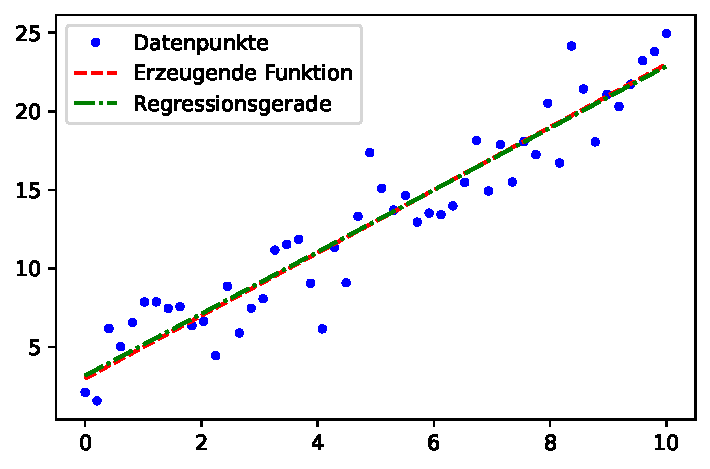
\includegraphics{aad_files/figure-pdf/fig-graphoflinearregression-output-2.pdf}

}

\caption{\label{fig-graphoflinearregression}Ausgleichsgerade.}

\end{figure}

\end{example}

\begin{center}\rule{0.5\linewidth}{0.5pt}\end{center}

\hypertarget{sec-deblurringImages}{%
\subsection{Bilder schärfen}\label{sec-deblurringImages}}

Die Idee zu dieser Anwendung stammt von Slater (2022). Beim
Fotografieren kann es passieren, dass die Linse der Kamera nicht richtig
fokussiert ist und das Bild dadurch unscharf wirkt. Es ist jedoch
möglich, ein Bild bis zu einem gewissen Grad nachträglich zu schärfen.

Als Testbild verwenden wir das folgende Bild eines Teddybären, welches
unter der Creative Commons 4.0 Lizenz auf
\url{https://www.pngall.com/toy-png/download/55843} {[}Letzter Zugriff
02.04.2023{]} zur Verfügung gestellt wird. Allerdings müssen wir die
Auflösung von ursprünglich 180 x 180 Pixel auf 30 x 30 Pixel reduzieren,
was mit jeder Bildbearbeitungssoftware gemacht werden kann. Der Grund
dafür ist, dass die Anzahl Pixel darüber entscheidet, wie viele
\texttt{FloatAad}-Objekte wir erzeugen müssen und während des Gradient
Descent Verfahrens wird der Computational Graph bei vielen Variablen
sehr gross, so dass beim Berechnen der Ableitungen die maximale
Rekursionstiefe überschritten würde. Wir verwenden also das in rechts
dargestellte Bild \texttt{Bear30.jpg}.

\begin{figure}

\begin{minipage}[b]{0.50\linewidth}

{\centering 

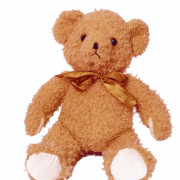
\includegraphics{Bear_original.png}

}

\subcaption{\label{fig-originalTeddy}Original 180 x 180}
\end{minipage}%
%
\begin{minipage}[b]{0.50\linewidth}

{\centering 


\includegraphics[width=1.875in,height=\textheight]{Bear30.jpg}

}

\subcaption{\label{fig-smallTeddy}Testbild 30 x 30}
\end{minipage}%

\caption{\label{fig-teddys}Testbild eines Teddybärs.}

\end{figure}

Es stellt sich heraus, dass selbst diese kleine Auflösung noch zu viele
\texttt{FloatAad}-Objekte benötigt weil jedes Pixel drei Farbkanäle hat.
Daher wandeln wir das Bild nach dem Laden zuerst in ein Graustufenbild
um.

\begin{Shaded}
\begin{Highlighting}[]
\ImportTok{from}\NormalTok{ matplotlib.image }\ImportTok{import}\NormalTok{ imread}
\ImportTok{from}\NormalTok{ floataad }\ImportTok{import}\NormalTok{ float2FloatAad, getGradient}

\ImportTok{import}\NormalTok{ matplotlib.pyplot }\ImportTok{as}\NormalTok{ plt}
\ImportTok{import}\NormalTok{ math}
\ImportTok{import}\NormalTok{ numpy }\ImportTok{as}\NormalTok{ np}

\NormalTok{original }\OperatorTok{=}\NormalTok{ imread(}\StringTok{\textquotesingle{}bear30.jpg\textquotesingle{}}\NormalTok{) }\OperatorTok{/} \DecValTok{255}
\CommentTok{\# Bild in Graustufenbild umwandeln}
\NormalTok{image }\OperatorTok{=} \DecValTok{1}\OperatorTok{/}\DecValTok{3} \OperatorTok{*}\NormalTok{ (original[:,:,}\DecValTok{0}\NormalTok{] }\OperatorTok{+}\NormalTok{ original[:,:,}\DecValTok{1}\NormalTok{] }\OperatorTok{+}\NormalTok{ original[:,:,}\DecValTok{2}\NormalTok{])}
\NormalTok{[length, width] }\OperatorTok{=}\NormalTok{ np.shape(image)}
\end{Highlighting}
\end{Shaded}

Um die Unschärfe einer schlecht fokussierten Linse zu simulieren, wenden
wir einen \emph{Gaussian Blur} an. Wie das genau funktioniert wird z.B.
in diesem Video von Grant Sanderson von
\href{https://www.3blue1brown.com}{3blue1brown} {[}Letzter Aufruf
02.04.2023{]} erklärt.

\url{https://youtu.be/KuXjwB4LzSA}

Die folgende Funktion wendet einen solchen Gaussian Blur auf ein Bild
an. Die Vorlage des Codes stammt aus dem Forumsbeitrag
\href{https://stackoverflow.com/questions/29920114/how-to-gauss-filter-blur-a-floating-point-numpy-array}{How
to gauss-filter (blur) a floating point numpy array} von stackoverflow
{[}Letzter Zugriff 02.04.2023{]} und wurde so abgeändert, dass die
kernel-Grösse selber bestimmt werden kann.

\begin{Shaded}
\begin{Highlighting}[]
\KeywordTok{def}\NormalTok{ blur(a): }
    \CommentTok{\# kernel erzeugen}
\NormalTok{    kernel\_size }\OperatorTok{=} \DecValTok{4}
\NormalTok{    k1 }\OperatorTok{=}\NormalTok{ [np.array([math.comb(kernel\_size, k) }\ControlFlowTok{for}\NormalTok{ k }\KeywordTok{in} \BuiltInTok{range}\NormalTok{(kernel\_size)])]}
\NormalTok{    kernel }\OperatorTok{=}\NormalTok{ np.dot(np.transpose(k1), k1)}
\NormalTok{    kernel }\OperatorTok{=}\NormalTok{ kernel }\OperatorTok{/}\NormalTok{ np.}\BuiltInTok{sum}\NormalTok{(kernel)}
    
    \CommentTok{\# Faltung (Convolution) ausführen}
\NormalTok{    arraylist }\OperatorTok{=}\NormalTok{ []}
    \ControlFlowTok{for}\NormalTok{ y }\KeywordTok{in} \BuiltInTok{range}\NormalTok{(kernel\_size):}
\NormalTok{        temparray }\OperatorTok{=}\NormalTok{ np.copy(a)}
\NormalTok{        temparray }\OperatorTok{=}\NormalTok{ np.roll(temparray, y }\OperatorTok{{-}} \DecValTok{1}\NormalTok{, axis}\OperatorTok{=}\DecValTok{0}\NormalTok{)}
        \ControlFlowTok{for}\NormalTok{ x }\KeywordTok{in} \BuiltInTok{range}\NormalTok{(kernel\_size):}
\NormalTok{            temparray\_X }\OperatorTok{=}\NormalTok{ np.copy(temparray)}
\NormalTok{            temparray\_X }\OperatorTok{=}\NormalTok{ np.roll(temparray\_X, x }\OperatorTok{{-}} \DecValTok{1}\NormalTok{, axis}\OperatorTok{=}\DecValTok{1}\NormalTok{)}\OperatorTok{*}\NormalTok{kernel[y,x]}
\NormalTok{            arraylist.append(temparray\_X)}

\NormalTok{    arraylist }\OperatorTok{=}\NormalTok{ np.array(arraylist)}
\NormalTok{    arraylist\_sum }\OperatorTok{=}\NormalTok{ np.}\BuiltInTok{sum}\NormalTok{(arraylist, axis}\OperatorTok{=}\DecValTok{0}\NormalTok{)}
    \ControlFlowTok{return}\NormalTok{ arraylist\_sum}
\end{Highlighting}
\end{Shaded}

Nun wenden wir diesen Filter auf unser Testbild an.

\begin{Shaded}
\begin{Highlighting}[]
\CommentTok{\# Blur erzeugen}
\NormalTok{blurredimage }\OperatorTok{=}\NormalTok{ blur(image)}
\NormalTok{blurrarray }\OperatorTok{=}\NormalTok{ np.reshape(blurredimage, length}\OperatorTok{*}\NormalTok{width)}

\CommentTok{\# Plot}
\NormalTok{ax }\OperatorTok{=}\NormalTok{ plt.subplot(}\DecValTok{1}\NormalTok{,}\DecValTok{2}\NormalTok{,}\DecValTok{1}\NormalTok{)}
\NormalTok{ax.set\_title(}\StringTok{"Original"}\NormalTok{)}
\NormalTok{ax.set\_axis\_off()}
\NormalTok{plt.imshow(image, cmap }\OperatorTok{=} \StringTok{"gray"}\NormalTok{)}

\NormalTok{ax }\OperatorTok{=}\NormalTok{ plt.subplot(}\DecValTok{1}\NormalTok{,}\DecValTok{2}\NormalTok{,}\DecValTok{2}\NormalTok{)}
\NormalTok{ax.set\_title(}\StringTok{"Blurred"}\NormalTok{)}
\NormalTok{ax.set\_axis\_off()}
\NormalTok{plt.imshow(blurredimage, cmap }\OperatorTok{=} \StringTok{"gray"}\NormalTok{)}

\NormalTok{plt.show()}
\end{Highlighting}
\end{Shaded}

\begin{figure}[H]

{\centering 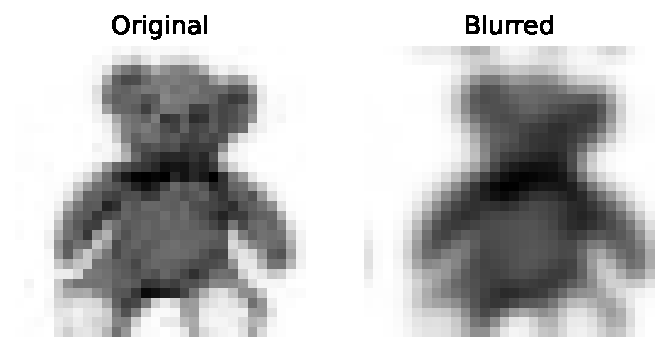
\includegraphics{aad_files/figure-pdf/fig-testbildmitblur-output-1.pdf}

}

\caption{\label{fig-testbildmitblur}Testbild und Blur.}

\end{figure}

Unser Ziel ist wie gesagt, mit Hilfe des Gradient Descent Verfahrens aus
dem unscharfen Bild rechts wieder so nahe wie möglich an das Original
heranzukommen. Dazu beginnen wir mit einem ``Startwert'', das ein Bild
ist, welches aus 30 x 30 Pixeln besteht, die alle den Wert 0.5 haben,
d.h. mit einem grauen Bild.

\begin{Shaded}
\begin{Highlighting}[]
\CommentTok{\# Startwert}
\NormalTok{guessimage }\OperatorTok{=}\NormalTok{ np.full(shape }\OperatorTok{=}\NormalTok{ [length, width], fill\_value}\OperatorTok{=}\FloatTok{0.5}\NormalTok{)}
\end{Highlighting}
\end{Shaded}

Diese \(30\times30=900\) Pixelwerte sind nun der Input unserer Loss
Funktion und werden im Laufe der Gradient Descent Iteration so
verändert, dass sie diese Funktion minimieren. Diese Loss Funktion
definieren wir folgendermassen: Auf das \texttt{guessimage} wird zuerst
ein Gaussian Blur angewendet. Danach betrachten wir die Differenzen
\texttt{blur(guessimage)\ -\ blurredimage} in jedem Pixel. Nach dem
Gauss'schen Ansatz der kleinsten Fehlerquadrate definieren wir die Loss
Funktion als Summe der Quadrate aller Fehler in den einzelnen Pixeln.
Dahinter steckt die Idee, dass wenn die Differenzen zwischen den
unscharfen Bildern \texttt{blur(guessimage)\ -\ blur(original)} klein
ist, dann sollten auch die Differenzen \texttt{guessimage\ -\ original}
klein sein, d.h. \texttt{testimage} sollte in etwa dem \texttt{original}
entsprechen.

Für die konkrete Umsetzung wandeln wir das Bild mit den \(30\times30\)
Pixeln in einen Vektor der Länge 900 um. Das haben wir für für das
\texttt{blurredimage} bereits in der Zeile
\texttt{blurrarray\ =\ np.reshape(blurredimage,\ length*width)} gemacht.
Für das \texttt{guessimage} müssen wir nach der Umwandlung die 900
Einträge zunächst in \texttt{FloatAad}-Objekte umwandeln. All das
geschieht in der folgenden Funktion.

\begin{Shaded}
\begin{Highlighting}[]
\KeywordTok{def}\NormalTok{ loss(x):}
    \CommentTok{\# Input x ist ein Bild, auf welches der Gauss Filter angewendet wird}
    \CommentTok{\# Danach wird das Bild als 1{-}dim. Array gespeichert}
\NormalTok{    [length, width] }\OperatorTok{=}\NormalTok{ np.shape(x)}
\NormalTok{    temp }\OperatorTok{=}\NormalTok{ blur(x)}
\NormalTok{    temparray }\OperatorTok{=}\NormalTok{ np.reshape(temp, length }\OperatorTok{*}\NormalTok{ width)}

    \CommentTok{\# Umwandeln in FloatAad}
\NormalTok{    temparray }\OperatorTok{=}\NormalTok{ float2FloatAad(temparray)}

\NormalTok{    y }\OperatorTok{=} \BuiltInTok{sum}\NormalTok{((temparray }\OperatorTok{{-}}\NormalTok{ blurrarray) }\OperatorTok{**} \DecValTok{2}\NormalTok{)}
\NormalTok{    g }\OperatorTok{=}\NormalTok{ getGradient(temparray, y)}
    \ControlFlowTok{return}\NormalTok{ [y.value, g]}
\end{Highlighting}
\end{Shaded}

Nun können wir das Gradient Descent Verfahren anwenden.

\begin{Shaded}
\begin{Highlighting}[]
\CommentTok{\# Gradient Descent Parameter}
\NormalTok{lam }\OperatorTok{=} \FloatTok{0.01}
\NormalTok{tol }\OperatorTok{=} \FloatTok{0.5}

\NormalTok{[lossval, grad] }\OperatorTok{=}\NormalTok{ loss(guessimage)}

\ControlFlowTok{while}\NormalTok{ lossval }\OperatorTok{\textgreater{}}\NormalTok{ tol:}
\NormalTok{    [lossval, grad] }\OperatorTok{=}\NormalTok{ loss(guessimage) }
\NormalTok{    diff }\OperatorTok{=}\NormalTok{ np.reshape(grad, [length, width])}
\NormalTok{    guessimage }\OperatorTok{=}\NormalTok{ guessimage }\OperatorTok{{-}}\NormalTok{ lam }\OperatorTok{*}\NormalTok{ diff}

\CommentTok{\# Plot}
\NormalTok{ax }\OperatorTok{=}\NormalTok{ plt.subplot(}\DecValTok{2}\NormalTok{,}\DecValTok{2}\NormalTok{,}\DecValTok{1}\NormalTok{)}
\NormalTok{ax.set\_title(}\StringTok{"Guess"}\NormalTok{)}
\NormalTok{ax.set\_axis\_off()}
\NormalTok{plt.imshow(guessimage, cmap }\OperatorTok{=} \StringTok{"gray"}\NormalTok{)}

\NormalTok{ax }\OperatorTok{=}\NormalTok{ plt.subplot(}\DecValTok{2}\NormalTok{,}\DecValTok{2}\NormalTok{,}\DecValTok{2}\NormalTok{)}
\NormalTok{ax.set\_title(}\StringTok{"Blurred Guess"}\NormalTok{)}
\NormalTok{ax.set\_axis\_off()}
\NormalTok{blurredguess }\OperatorTok{=}\NormalTok{ blur(guessimage)}
\NormalTok{plt.imshow(blurredguess, cmap }\OperatorTok{=} \StringTok{"gray"}\NormalTok{)}

\NormalTok{ax }\OperatorTok{=}\NormalTok{ plt.subplot(}\DecValTok{2}\NormalTok{,}\DecValTok{2}\NormalTok{,}\DecValTok{3}\NormalTok{)}
\NormalTok{ax.set\_title(}\StringTok{"Original {-} Guess"}\NormalTok{)}
\NormalTok{ax.set\_axis\_off()}
\NormalTok{diffOrig }\OperatorTok{=} \FloatTok{0.5} \OperatorTok{*}\NormalTok{ (image }\OperatorTok{{-}}\NormalTok{ guessimage }\OperatorTok{+} \DecValTok{1}\NormalTok{)}
\NormalTok{plt.imshow(diffOrig, cmap }\OperatorTok{=} \StringTok{"gray"}\NormalTok{)}

\NormalTok{ax }\OperatorTok{=}\NormalTok{ plt.subplot(}\DecValTok{2}\NormalTok{,}\DecValTok{2}\NormalTok{,}\DecValTok{4}\NormalTok{)}
\NormalTok{ax.set\_title(}\StringTok{"Blurred {-} Blurred Guess"}\NormalTok{)}
\NormalTok{ax.set\_axis\_off()}
\NormalTok{diffBlurred }\OperatorTok{=} \FloatTok{0.5} \OperatorTok{*}\NormalTok{ (blurredimage }\OperatorTok{{-}}\NormalTok{ blurredguess }\OperatorTok{+} \DecValTok{1}\NormalTok{)}
\NormalTok{plt.imshow(diffBlurred, cmap }\OperatorTok{=} \StringTok{"gray"}\NormalTok{)}

\NormalTok{plt.show()}
\end{Highlighting}
\end{Shaded}

\begin{figure}[H]

{\centering 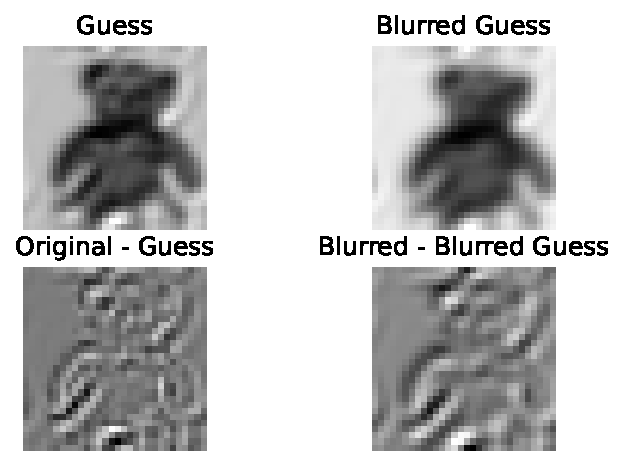
\includegraphics{aad_files/figure-pdf/fig-imagereconstructionresult-output-1.pdf}

}

\caption{\label{fig-imagereconstructionresult}Resultat des Schärfens und
Differenz zum Original}

\end{figure}

Das vollständige Programm kann auch \href{deblurImage.py}{hier}
heruntergeladen werden.

\hypertarget{sec-modulMathAad}{%
\section{\texorpdfstring{Das Modul
\texttt{mathaad}}{Das Modul mathaad}}\label{sec-modulMathAad}}

In diesem Kapitel schreiben wir ein Modul \texttt{mathaad}, welches eine
Auswahl an mathematischen Funktionen beinhaltet, die auf
\texttt{FloatAad}-Objekte angewendet werden können. Wir gehen dabei
analog zum Kapitel~\ref{sec-modulMathSad} vor, beschränken uns aber auf
die Funktionen \texttt{sqrt}, \texttt{exp}, \texttt{log} und die drei
trigonometrischen Funktionen. Ausserdem verwenden wir Funktionen aus
\texttt{numpy} weil wir als Argumente auch Arrays von
\texttt{FloatAad}-Objekte übergeben wollen. Die Funktion soll in diesem
Fall elementweise angewendet werden, wofür der Decorator
\texttt{@np.vectorize} sorg. Der folgende Code sollte in einer Datei
\texttt{mathaad.py} gespeichert und im gleichen Ordner wie die anderen
Dateien abgelegt werden.

\begin{Shaded}
\begin{Highlighting}[]
\ImportTok{import}\NormalTok{ numpy }\ImportTok{as}\NormalTok{ np}
\ImportTok{from}\NormalTok{ floataad }\ImportTok{import}\NormalTok{ FloatAad}

\AttributeTok{@np.vectorize}
\KeywordTok{def}\NormalTok{ sqrt(x):}
\NormalTok{    newValue }\OperatorTok{=}\NormalTok{ np.sqrt(x.value)}
\NormalTok{    newDerivative }\OperatorTok{=}\NormalTok{ (}
\NormalTok{        (x, }\FloatTok{1.} \OperatorTok{/}\NormalTok{ (}\DecValTok{2} \OperatorTok{*}\NormalTok{ np.sqrt(x.value))),}
\NormalTok{    )}
    \ControlFlowTok{return}\NormalTok{ FloatAad(newValue, newDerivative)}

\AttributeTok{@np.vectorize}
\KeywordTok{def}\NormalTok{ exp(x):}
\NormalTok{    newValue }\OperatorTok{=}\NormalTok{ np.exp(x.value)}
\NormalTok{    newDerivative }\OperatorTok{=}\NormalTok{ (}
\NormalTok{        (x, newValue),}
\NormalTok{    )}
    \ControlFlowTok{return}\NormalTok{ FloatAad(newValue, newDerivative)}

\AttributeTok{@np.vectorize}
\KeywordTok{def}\NormalTok{ log(x):}
\NormalTok{    newValue }\OperatorTok{=}\NormalTok{ np.log(x.value)}
\NormalTok{    newDerivative }\OperatorTok{=}\NormalTok{ (}
\NormalTok{        (x, }\FloatTok{1.} \OperatorTok{/}\NormalTok{ x.value),}
\NormalTok{    )}
    \ControlFlowTok{return}\NormalTok{ FloatAad(newValue, newDerivative)}

\AttributeTok{@np.vectorize}
\KeywordTok{def}\NormalTok{ sin(x):}
\NormalTok{    newValue }\OperatorTok{=}\NormalTok{ np.sin(x.value)}
\NormalTok{    newDerivative }\OperatorTok{=}\NormalTok{ (}
\NormalTok{        (x, np.cos(x.value)),}
\NormalTok{    )}
    \ControlFlowTok{return}\NormalTok{ FloatAad(newValue, newDerivative)}

\AttributeTok{@np.vectorize}
\KeywordTok{def}\NormalTok{ cos(x):}
\NormalTok{    newValue }\OperatorTok{=}\NormalTok{ np.cos(x.value)}
\NormalTok{    newDerivative }\OperatorTok{=}\NormalTok{ (}
\NormalTok{        (x, }\OperatorTok{{-}}\NormalTok{np.sin(x.value)),}
\NormalTok{    )}
    \ControlFlowTok{return}\NormalTok{ FloatAad(newValue, newDerivative)}

\AttributeTok{@np.vectorize}
\KeywordTok{def}\NormalTok{ tan(x):}
    \ControlFlowTok{return}\NormalTok{ sin(x) }\OperatorTok{/}\NormalTok{ cos(x)}
\end{Highlighting}
\end{Shaded}

Die Datei kann \href{mathaad.py}{hier} heruntergeladen werden.

\hypertarget{das-modul-mathaad-im-einsatz}{%
\section{\texorpdfstring{Das Modul \texttt{mathaad} im
Einsatz}{Das Modul mathaad im Einsatz}}\label{das-modul-mathaad-im-einsatz}}

Zum Schluss wollen wir uns ein einfaches neuronales Netz zur Lösung
eines berühmten Klassifikationsproblems programmieren.

\hypertarget{ein-einaches-neuronales-netz-zur-klassifikation-von-lilien}{%
\subsection{Ein einaches neuronales Netz zur Klassifikation von
Lilien}\label{ein-einaches-neuronales-netz-zur-klassifikation-von-lilien}}

Wir verwenden für dieses Beispiel einen der bekanntesten Datensätze,
nämlich Fisher's Datensatz zu Lilien. Er wurde bereits 1936 vom
britischen Biologen und Statistier Ronald Fisher verwendet und ist heute
nach ihm benannt. Auch in Barot u.~a. (2022) (S. 160) wird auf diesen
Datensatz Bezug genommen. Die Datei \url{iris.data} kann von Fisher
(1936) heruntergeladen werden. Über diesen Datensatz liest man dort

\begin{quote}
{[}It is{]} A small classic dataset from Fisher, 1936. One of the
earliest datasets used for evaluation of classification methodologies.
{[}\ldots{]} This is perhaps the best known database to be found in the
pattern recognition literature. Fisher's paper is a classic in the field
and is referenced frequently to this day.
\end{quote}

Die Datei enthält 150 Datensätze (Zeilen) mit je 5 Spalten. Die 1.
Spalte gibt die Länge des Kelchblattes (Sepalum) an, die 2. Spalte die
Breite des Kelchblattes, die 3. Spalte enthält die Länge des Kornblattes
(Petalum) und die 4. Spalte enthält die Breite des Kornblattes. Die 5.
Spalte schliesslich gibt an, von welcher Lilienart die Daten stammen. Im
Datensatz gibt es drei Arten von Lilien (Iris setosa, Iris versicolor
und Iris virginica) und von jeder Art sind 50 Messungen enthalten.

Unser Ziel wird es sein, auf Grund der vier gemessenen Grössen (Länge
und Breite des Kelch- bzw. Kornblattes) die Art vorher zu sagen. Als
erstes wollen wir die Daten grafisch als Scatterplot darstellen (Frochte
(2021), S. 71). Zunächst ändern wir aber die Label in der 5. Spalte noch
zu \texttt{0} (Iris setosa), \texttt{1} (Iris versicolor), bzw.
\texttt{2} (Iris virginica)

\begin{Shaded}
\begin{Highlighting}[]
\ImportTok{import}\NormalTok{ numpy }\ImportTok{as}\NormalTok{ np}
\ImportTok{import}\NormalTok{ matplotlib.pyplot }\ImportTok{as}\NormalTok{ plt}
\ImportTok{from}\NormalTok{ time }\ImportTok{import}\NormalTok{ time}

\ImportTok{from}\NormalTok{ floataad }\ImportTok{import}\NormalTok{ float2FloatAad, getValues, getGradient}
\ImportTok{import}\NormalTok{ mathaad}

\CommentTok{\# Daten einlesen und Labels ändern}
\NormalTok{fString }\OperatorTok{=} \BuiltInTok{open}\NormalTok{(}\StringTok{\textquotesingle{}iris.data\textquotesingle{}}\NormalTok{,}\StringTok{\textquotesingle{}r\textquotesingle{}}\NormalTok{)}
\NormalTok{fFloat  }\OperatorTok{=} \BuiltInTok{open}\NormalTok{(}\StringTok{\textquotesingle{}iris.csv\textquotesingle{}}\NormalTok{,}\StringTok{\textquotesingle{}w\textquotesingle{}}\NormalTok{)}

\ControlFlowTok{for}\NormalTok{ line }\KeywordTok{in}\NormalTok{ fString:}
\NormalTok{    line }\OperatorTok{=}\NormalTok{ line.replace(}\StringTok{\textquotesingle{}Iris{-}setosa\textquotesingle{}}\NormalTok{, }\StringTok{\textquotesingle{}0\textquotesingle{}}\NormalTok{)}
\NormalTok{    line }\OperatorTok{=}\NormalTok{ line.replace(}\StringTok{\textquotesingle{}Iris{-}versicolor\textquotesingle{}}\NormalTok{, }\StringTok{\textquotesingle{}1\textquotesingle{}}\NormalTok{)}
\NormalTok{    line }\OperatorTok{=}\NormalTok{ line.replace(}\StringTok{\textquotesingle{}Iris{-}virginica\textquotesingle{}}\NormalTok{, }\StringTok{\textquotesingle{}2\textquotesingle{}}\NormalTok{)}
\NormalTok{    fFloat.write(line)}

\NormalTok{fString.close()}
\NormalTok{fFloat.close()}

\NormalTok{fFloat }\OperatorTok{=} \BuiltInTok{open}\NormalTok{(}\StringTok{\textquotesingle{}iris.csv\textquotesingle{}}\NormalTok{,}\StringTok{\textquotesingle{}r\textquotesingle{}}\NormalTok{)}
\NormalTok{dataset }\OperatorTok{=}\NormalTok{ np.loadtxt(fFloat, delimiter }\OperatorTok{=} \StringTok{\textquotesingle{},\textquotesingle{}}\NormalTok{)}
\NormalTok{fFloat.close()}

\CommentTok{\# Daten plotten}
\NormalTok{fig }\OperatorTok{=}\NormalTok{ plt.figure(}\DecValTok{1}\NormalTok{)}

\NormalTok{ax }\OperatorTok{=}\NormalTok{ fig.add\_subplot(}\DecValTok{2}\NormalTok{,}\DecValTok{2}\NormalTok{,}\DecValTok{1}\NormalTok{)}
\NormalTok{ax.scatter(dataset[}\DecValTok{0}\NormalTok{:}\DecValTok{50}\NormalTok{,}\DecValTok{0}\NormalTok{], dataset[}\DecValTok{0}\NormalTok{:}\DecValTok{50}\NormalTok{,}\DecValTok{1}\NormalTok{], }
\NormalTok{            c }\OperatorTok{=} \StringTok{\textquotesingle{}red\textquotesingle{}}\NormalTok{, s }\OperatorTok{=} \DecValTok{20}\NormalTok{, alpha }\OperatorTok{=} \FloatTok{0.6}\NormalTok{)}
\NormalTok{ax.scatter(dataset[}\DecValTok{50}\NormalTok{:}\DecValTok{100}\NormalTok{,}\DecValTok{0}\NormalTok{], dataset[}\DecValTok{50}\NormalTok{:}\DecValTok{100}\NormalTok{,}\DecValTok{1}\NormalTok{], }
\NormalTok{            c }\OperatorTok{=} \StringTok{\textquotesingle{}green\textquotesingle{}}\NormalTok{, marker }\OperatorTok{=} \StringTok{\textquotesingle{}\^{}\textquotesingle{}}\NormalTok{, s }\OperatorTok{=} \DecValTok{20}\NormalTok{, alpha }\OperatorTok{=} \FloatTok{0.6}\NormalTok{)}
\NormalTok{ax.scatter(dataset[}\DecValTok{100}\NormalTok{:}\DecValTok{150}\NormalTok{,}\DecValTok{0}\NormalTok{], dataset[}\DecValTok{100}\NormalTok{:}\DecValTok{150}\NormalTok{,}\DecValTok{1}\NormalTok{], }
\NormalTok{            c }\OperatorTok{=} \StringTok{\textquotesingle{}blue\textquotesingle{}}\NormalTok{, marker }\OperatorTok{=} \StringTok{\textquotesingle{}*\textquotesingle{}}\NormalTok{, s }\OperatorTok{=} \DecValTok{20}\NormalTok{, alpha }\OperatorTok{=} \FloatTok{0.6}\NormalTok{)}
\NormalTok{ax.set\_xlabel(}\StringTok{\textquotesingle{}Kelchblattlaenge (cm)\textquotesingle{}}\NormalTok{)}
\NormalTok{ax.set\_ylabel(}\StringTok{\textquotesingle{}Kelchblattbreite (cm)\textquotesingle{}}\NormalTok{)}

\NormalTok{ax }\OperatorTok{=}\NormalTok{ fig.add\_subplot(}\DecValTok{2}\NormalTok{,}\DecValTok{2}\NormalTok{,}\DecValTok{2}\NormalTok{)}
\NormalTok{ax.scatter(dataset[}\DecValTok{0}\NormalTok{:}\DecValTok{50}\NormalTok{,}\DecValTok{2}\NormalTok{], dataset[}\DecValTok{0}\NormalTok{:}\DecValTok{50}\NormalTok{,}\DecValTok{3}\NormalTok{], }
\NormalTok{            c }\OperatorTok{=} \StringTok{\textquotesingle{}red\textquotesingle{}}\NormalTok{, s }\OperatorTok{=} \DecValTok{20}\NormalTok{, alpha }\OperatorTok{=} \FloatTok{0.6}\NormalTok{)}
\NormalTok{ax.scatter(dataset[}\DecValTok{50}\NormalTok{:}\DecValTok{100}\NormalTok{,}\DecValTok{2}\NormalTok{], dataset[}\DecValTok{50}\NormalTok{:}\DecValTok{100}\NormalTok{,}\DecValTok{3}\NormalTok{], }
\NormalTok{            c }\OperatorTok{=} \StringTok{\textquotesingle{}green\textquotesingle{}}\NormalTok{, marker }\OperatorTok{=} \StringTok{\textquotesingle{}\^{}\textquotesingle{}}\NormalTok{, s }\OperatorTok{=} \DecValTok{20}\NormalTok{, alpha }\OperatorTok{=} \FloatTok{0.6}\NormalTok{)}
\NormalTok{ax.scatter(dataset[}\DecValTok{100}\NormalTok{:}\DecValTok{150}\NormalTok{,}\DecValTok{2}\NormalTok{], dataset[}\DecValTok{100}\NormalTok{:}\DecValTok{150}\NormalTok{,}\DecValTok{3}\NormalTok{], }
\NormalTok{            c }\OperatorTok{=} \StringTok{\textquotesingle{}blue\textquotesingle{}}\NormalTok{, marker }\OperatorTok{=} \StringTok{\textquotesingle{}*\textquotesingle{}}\NormalTok{, s }\OperatorTok{=} \DecValTok{20}\NormalTok{, alpha }\OperatorTok{=} \FloatTok{0.6}\NormalTok{)}
\NormalTok{ax.set\_xlabel(}\StringTok{\textquotesingle{}Kronblattlaenge (cm)\textquotesingle{}}\NormalTok{)}
\NormalTok{ax.set\_ylabel(}\StringTok{\textquotesingle{}Kronblattbreite (cm)\textquotesingle{}}\NormalTok{)}

\NormalTok{ax }\OperatorTok{=}\NormalTok{ fig.add\_subplot(}\DecValTok{2}\NormalTok{,}\DecValTok{2}\NormalTok{,}\DecValTok{3}\NormalTok{)}
\NormalTok{ax.scatter(dataset[}\DecValTok{0}\NormalTok{:}\DecValTok{50}\NormalTok{,}\DecValTok{0}\NormalTok{], dataset[}\DecValTok{0}\NormalTok{:}\DecValTok{50}\NormalTok{,}\DecValTok{2}\NormalTok{], }
\NormalTok{            c }\OperatorTok{=} \StringTok{\textquotesingle{}red\textquotesingle{}}\NormalTok{, s }\OperatorTok{=} \DecValTok{20}\NormalTok{, alpha }\OperatorTok{=} \FloatTok{0.6}\NormalTok{)}
\NormalTok{ax.scatter(dataset[}\DecValTok{50}\NormalTok{:}\DecValTok{100}\NormalTok{,}\DecValTok{0}\NormalTok{], dataset[}\DecValTok{50}\NormalTok{:}\DecValTok{100}\NormalTok{,}\DecValTok{2}\NormalTok{], }
\NormalTok{            c }\OperatorTok{=} \StringTok{\textquotesingle{}green\textquotesingle{}}\NormalTok{, marker }\OperatorTok{=} \StringTok{\textquotesingle{}\^{}\textquotesingle{}}\NormalTok{, s }\OperatorTok{=} \DecValTok{20}\NormalTok{, alpha }\OperatorTok{=} \FloatTok{0.6}\NormalTok{)}
\NormalTok{ax.scatter(dataset[}\DecValTok{100}\NormalTok{:}\DecValTok{150}\NormalTok{,}\DecValTok{0}\NormalTok{], dataset[}\DecValTok{100}\NormalTok{:}\DecValTok{150}\NormalTok{,}\DecValTok{2}\NormalTok{], }
\NormalTok{            c }\OperatorTok{=} \StringTok{\textquotesingle{}blue\textquotesingle{}}\NormalTok{, marker }\OperatorTok{=} \StringTok{\textquotesingle{}*\textquotesingle{}}\NormalTok{, s }\OperatorTok{=} \DecValTok{20}\NormalTok{, alpha }\OperatorTok{=} \FloatTok{0.6}\NormalTok{)}
\NormalTok{ax.set\_xlabel(}\StringTok{\textquotesingle{}Kelchblattlaenge (cm)\textquotesingle{}}\NormalTok{)}
\NormalTok{ax.set\_ylabel(}\StringTok{\textquotesingle{}Kronblattlaenge (cm)\textquotesingle{}}\NormalTok{)}

\NormalTok{ax }\OperatorTok{=}\NormalTok{ fig.add\_subplot(}\DecValTok{2}\NormalTok{,}\DecValTok{2}\NormalTok{,}\DecValTok{4}\NormalTok{)}
\NormalTok{ax.scatter(dataset[}\DecValTok{0}\NormalTok{:}\DecValTok{50}\NormalTok{,}\DecValTok{1}\NormalTok{], dataset[}\DecValTok{0}\NormalTok{:}\DecValTok{50}\NormalTok{,}\DecValTok{3}\NormalTok{], }
\NormalTok{            c }\OperatorTok{=} \StringTok{\textquotesingle{}red\textquotesingle{}}\NormalTok{, s }\OperatorTok{=} \DecValTok{20}\NormalTok{, alpha }\OperatorTok{=} \FloatTok{0.6}\NormalTok{)}
\NormalTok{ax.scatter(dataset[}\DecValTok{50}\NormalTok{:}\DecValTok{100}\NormalTok{,}\DecValTok{1}\NormalTok{], dataset[}\DecValTok{50}\NormalTok{:}\DecValTok{100}\NormalTok{,}\DecValTok{3}\NormalTok{], }
\NormalTok{            c }\OperatorTok{=} \StringTok{\textquotesingle{}green\textquotesingle{}}\NormalTok{, marker }\OperatorTok{=} \StringTok{\textquotesingle{}\^{}\textquotesingle{}}\NormalTok{, s }\OperatorTok{=} \DecValTok{20}\NormalTok{, alpha }\OperatorTok{=} \FloatTok{0.6}\NormalTok{)}
\NormalTok{ax.scatter(dataset[}\DecValTok{100}\NormalTok{:}\DecValTok{150}\NormalTok{,}\DecValTok{1}\NormalTok{], dataset[}\DecValTok{100}\NormalTok{:}\DecValTok{150}\NormalTok{,}\DecValTok{3}\NormalTok{], }
\NormalTok{            c }\OperatorTok{=} \StringTok{\textquotesingle{}blue\textquotesingle{}}\NormalTok{, marker }\OperatorTok{=} \StringTok{\textquotesingle{}*\textquotesingle{}}\NormalTok{, s }\OperatorTok{=} \DecValTok{20}\NormalTok{, alpha }\OperatorTok{=} \FloatTok{0.6}\NormalTok{)}
\NormalTok{ax.set\_xlabel(}\StringTok{\textquotesingle{}Kelchblattbreite (cm)\textquotesingle{}}\NormalTok{)}
\NormalTok{ax.set\_ylabel(}\StringTok{\textquotesingle{}Kronblattbreite (cm)\textquotesingle{}}\NormalTok{)}

\NormalTok{plt.show()}
\end{Highlighting}
\end{Shaded}

\begin{figure}[H]

{\centering 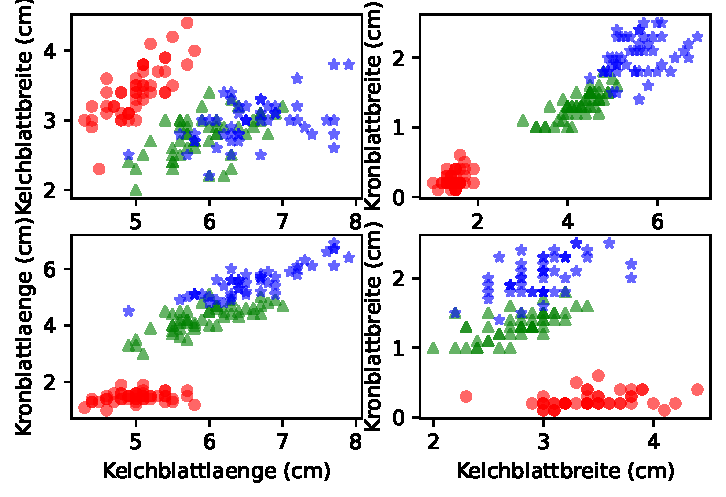
\includegraphics{aad_files/figure-pdf/fig-imageirisscatterplot-output-1.pdf}

}

\caption{\label{fig-imageirisscatterplot}Scatter Plots der Fisher Iris
Daten}

\end{figure}

Nun wählen wir uns aus den 150 Einträgen des Datensatzes zufällig 30
heraus, welche wir als Testdaten verwenden. Die übrigen 120 Einträge
dienen uns als Trainingsdaten, mit denen wir unser neuronales Netz
trainieren werden.

\begin{Shaded}
\begin{Highlighting}[]
\CommentTok{\# Daten in Trainings{-} und Testdaten aufteilen}
\NormalTok{X }\OperatorTok{=}\NormalTok{ dataset[:, }\DecValTok{0}\NormalTok{:}\DecValTok{4}\NormalTok{] }\CommentTok{\# Messwerte}
\NormalTok{Y }\OperatorTok{=}\NormalTok{ dataset[:, }\DecValTok{4}\NormalTok{]   }\CommentTok{\# Label}
\NormalTok{allData }\OperatorTok{=}\NormalTok{ np.arange(}\DecValTok{0}\NormalTok{, X.shape[}\DecValTok{0}\NormalTok{])}
\NormalTok{testIndices }\OperatorTok{=}\NormalTok{ np.random.choice(X.shape[}\DecValTok{0}\NormalTok{], size }\OperatorTok{=} \DecValTok{30}\NormalTok{, replace }\OperatorTok{=} \VariableTok{False}\NormalTok{)}
\NormalTok{trainIndices }\OperatorTok{=}\NormalTok{ np.delete(allData, testIndices)}
\NormalTok{dataRecords }\OperatorTok{=} \BuiltInTok{len}\NormalTok{(testIndices)}
\NormalTok{XTrain }\OperatorTok{=}\NormalTok{ X[trainIndices, :]}
\NormalTok{YTrain }\OperatorTok{=}\NormalTok{ np.array(Y[trainIndices], dtype }\OperatorTok{=}\NormalTok{ np.int32)}
\NormalTok{XTest }\OperatorTok{=}\NormalTok{ X[testIndices, :]}
\NormalTok{YTest }\OperatorTok{=}\NormalTok{ Y[testIndices]}
\end{Highlighting}
\end{Shaded}

Unser Netz soll aus 4 Inputneuronen und 3 Outputneuronen bestehen. Die
vier Inputs stehen für die vier Messwerte
\texttt{X{[}0{]},\ ...,\ X{[}3{]}}. Wenn dort die entsprechenden
Messwerte eingegeben wurden, dann werden bei den Outputneuronen
\texttt{Y{[}0{]},\ ...,\ Y{[}2{]}} vier Werte zwischen \(0\) und \(1\)
generiert, welche die Wahrscheinlichkeiten darstellen, dass es sich um
die entsprechende Lilienart handelt. Das Neuron mit dem grössten Wert
stellt unsere Vorhersage dar. Das neuronale Netz hat also die folgende
Architektur:

\begin{figure}

{\centering 

\begin{figure}[H]

{\centering \includegraphics[width=4in,height=3.5in]{aad_files/figure-latex/dot-figure-2.png}

}

\end{figure}

}

\caption{\label{fig-FisherNNArchitecture}Neuronales Netz für den
Lilienklassifikator.}

\end{figure}

Entlang jeder Kante multiplizeren wir den Wert \(x_i\) mit einem Gewicht
\(w_{ij}\) und addieren die vier Werte. Zu dieser Summe addieren wir
noch einen Bias \(b_i\) so entstehen drei Zwischenwerte \[
z_i = \sum_{j=0}^3 w_{ij}x_j + b_i \quad\textrm{für}\quad i\in\lbrace0, 1, 2\rbrace
\] In Matrixschreibweise können wir das ausdrücken als \[
\vec{z} = W\cdot \vec{x} + \vec{b}
\] mit \(W\in \mathbb{R}^{3\times 4}\), \(\vec{x}\in\mathbb{R}^4\) und
\(\vec{b}, \vec{z} \in \mathbb{R}^3\). Die Zwischenwerten \(z_i\) müssen
nun noch so skaliert werden, dass sie eine Wahrscheinlichkeitsverteilung
darstellen. Das erreichen wir, die Softmax Funktion anwenden: \[
\hat y_i = \sigma_i(\vec z) = \frac{e^{z_i}}{\sum_{k=0}^2 e^{z_k}} \quad\textrm{für}\quad i\in\lbrace0, 1, 2\rbrace
\] Mehr zur Softmax Funktion findet man z.B. in Frochte (2021) (S. 240).
Im folgenden Programm unterscheiden wir noch, ob wir die Funktion auf
einen Vektor aus Zahlen oder einen Vektor aus \texttt{FloatAad}-Objekten
anwenden.

\begin{Shaded}
\begin{Highlighting}[]
\CommentTok{\# Softmax Funktion für Vektor z}
\KeywordTok{def}\NormalTok{ softmax(z):}
    \ControlFlowTok{if}\NormalTok{ z.dtype }\OperatorTok{==} \StringTok{"object"}\NormalTok{:}
        \ControlFlowTok{return}\NormalTok{ [mathaad.exp(x) }\OperatorTok{/} \BuiltInTok{sum}\NormalTok{(mathaad.exp(z)) }\ControlFlowTok{for}\NormalTok{ x }\KeywordTok{in}\NormalTok{ z]}
    \ControlFlowTok{else}\NormalTok{:}
        \ControlFlowTok{return}\NormalTok{ [np.exp(x) }\OperatorTok{/} \BuiltInTok{sum}\NormalTok{(np.exp(z)) }\ControlFlowTok{for}\NormalTok{ x }\KeywordTok{in}\NormalTok{ z]}
\end{Highlighting}
\end{Shaded}

Unsere Vorhersage ist dann der Wert \[
y = \operatorname{argmax} \hat y_i \in \lbrace0, 1, 2\rbrace 
\]

Die Frage ist also, wie wir die 12 Gewichte \(w_{ij}\) und die Bias
\(b_i\) wählen. Letztere setzen wir einfach auf \(b_i = 1\) für alle
\(i\). Bei der Bestimmung der Gewichte kommen unsere Trainingsdaten ins
Spiel. Wir definieren uns eine Loss Funktion
\(J : \mathbb{R}^{12} \rightarrow \mathbb{R}\), welche als Input die
Gewichte \(W\) erhält und als Output die so genannte Cross-Entropy
liefert, welche ein Mass für die Abweichung von der korrekten
Klassifikation ist. Sie wird bestimmt, indem man zuerst \[
D(\vec y, \vec {\hat y}) = - \sum_i y_i\cdot \ln(\hat y_i)
\] berechnet, wobei die \(\hat y_i\) wie oben definiert sind und
\(\vec y = (y_i)_{i=0, 1, 2}\) die One-Hot Codierung der korrekten
Labels ist, d.h. \begin{align*}
    \vec y &= (\matrix{1, 0, 0})^\intercal \quad\textrm{falls der korrekte Label 0 (Iris setosa) ist,} \\
    \vec y &= (\matrix{0, 1, 0})^\intercal \quad\textrm{falls der korrekte Label 1 (Iris versicolor) ist,} \\ 
    \vec y &= (\matrix{0, 0, 1})^\intercal \quad\textrm{falls der korrekte Label 2 (Iris virginica) ist.}
\end{align*}

Die Cross-Entropy über alle \(N=120\) Beispiele erhält man dann als
Mittelwert dieser Grössen \[
J(W) = \frac{1}{N}\sum_{n=0}^{N-1} D(\vec y^{(n)}, \vec{\hat y}^{(n)})
\] Weitere Details zur Cross-Entropy findet man ebenfalls in Frochte
(2021) (S. 241). In der Python Funktion wandeln wir die Gewichte zuerst
in \texttt{FloatAad}-Objete um und geben am Schluss den Wert \(J(W)\)
und die den Gradienten \(\nabla J (W)\) zurück.

\begin{Shaded}
\begin{Highlighting}[]
\KeywordTok{def}\NormalTok{ loss(Weights, bias, XTrain, YTrain):}
    
\NormalTok{    N }\OperatorTok{=} \BuiltInTok{len}\NormalTok{(YTrain) }\CommentTok{\# Anzahl Trainingsdaten}
    
    \CommentTok{\# Gewichte als FloatAad{-}Matrix}
\NormalTok{    Wtemp }\OperatorTok{=}\NormalTok{ float2FloatAad(Weights)}
\NormalTok{    WtempMatrix }\OperatorTok{=}\NormalTok{ np.reshape(Wtemp, [}\DecValTok{4}\NormalTok{, }\DecValTok{3}\NormalTok{])}
    
    
    \CommentTok{\# Labels als One{-}Hot Encoding}
\NormalTok{    YOneHot }\OperatorTok{=}\NormalTok{ np.zeros([N, }\DecValTok{3}\NormalTok{])}
\NormalTok{    YOneHot[}\BuiltInTok{range}\NormalTok{(N), YTrain] }\OperatorTok{=} \DecValTok{1}

\NormalTok{    Z }\OperatorTok{=}\NormalTok{ XTrain }\OperatorTok{@}\NormalTok{ WtempMatrix }\OperatorTok{+}\NormalTok{ bias}
    \CommentTok{\# Softmax auf jede Zeile anwenden}
\NormalTok{    Yhat }\OperatorTok{=}\NormalTok{ np.apply\_along\_axis(softmax, }\DecValTok{1}\NormalTok{, Z)}
    
    \CommentTok{\# Cross Entropy}
\NormalTok{    D }\OperatorTok{=}\NormalTok{ [}\OperatorTok{{-}}\NormalTok{ YOneHot[i] }\OperatorTok{@}\NormalTok{ mathaad.log(Yhat[i]) }\ControlFlowTok{for}\NormalTok{ i }\KeywordTok{in} \BuiltInTok{range}\NormalTok{(N) ]}
\NormalTok{    J }\OperatorTok{=} \BuiltInTok{sum}\NormalTok{(D) }\OperatorTok{/}\NormalTok{ N}
\NormalTok{    LossValue }\OperatorTok{=}\NormalTok{ getValues(J)}
\NormalTok{    LossGrad }\OperatorTok{=}\NormalTok{ np.array(getGradient(Wtemp, J))}
    \ControlFlowTok{return}\NormalTok{ [LossValue, LossGrad]}
\end{Highlighting}
\end{Shaded}

Man beachte, dass das Matrixprodukt in der Zeile
\texttt{Z\ =\ XTrain\ @\ WtempMatrix\ +\ bias} eigentlich
\(X\cdot W^\intercal + \vec b^\intercal\) ist, mit
\(X\in\mathbb{R}^{120\times 4}\) und
\(W^\intercal \in \mathbb{R}^{4\times 3}\). Die Addition von
\texttt{bias} wird dann auf jede Zeile
\(X\cdot W^\intercal \in \mathbb{R}^{120\times 3}\) angewendet.

Nun verwenden wir wieder das Gradient Descent Verfahren, um ein lokales
Minimum der Loss Funktion zu finden und damit die Gewichte zu
optimieren. Wir initialisieren die Gewichte mit zufälligen Werten.

\begin{Shaded}
\begin{Highlighting}[]
\CommentTok{\# Gewichte initialisieren}
\NormalTok{W }\OperatorTok{=}\NormalTok{ np.random.random(}\DecValTok{4} \OperatorTok{*} \DecValTok{3}\NormalTok{)}
\NormalTok{b }\OperatorTok{=}\NormalTok{ np.ones(}\DecValTok{3}\NormalTok{)  }\CommentTok{\# bias}

\CommentTok{\# Fit mit Gradient Descent}
\NormalTok{lam }\OperatorTok{=} \FloatTok{0.5} \CommentTok{\# Lernrate}
\NormalTok{tol }\OperatorTok{=} \FloatTok{1e{-}2}
\NormalTok{start }\OperatorTok{=}\NormalTok{ time()}
\NormalTok{[Lval, Lgrad] }\OperatorTok{=}\NormalTok{ loss(W, b, XTrain, YTrain)}
\ControlFlowTok{while}\NormalTok{ np.linalg.norm(Lgrad) }\OperatorTok{\textgreater{}}\NormalTok{ tol:}
\NormalTok{    W1 }\OperatorTok{=}\NormalTok{ W }\OperatorTok{{-}}\NormalTok{ lam }\OperatorTok{*}\NormalTok{ Lgrad}
\NormalTok{    [Lval, Lgrad] }\OperatorTok{=}\NormalTok{ loss(W1, b, XTrain, YTrain)}
\NormalTok{    W }\OperatorTok{=}\NormalTok{ W1}
\NormalTok{end }\OperatorTok{=}\NormalTok{ time()}
\NormalTok{zeit }\OperatorTok{=}\NormalTok{ end }\OperatorTok{{-}}\NormalTok{ start}
\BuiltInTok{print}\NormalTok{(}\StringTok{"Der Lernprozess dauerte }\SpecialCharTok{\%1.2f}\StringTok{ Sekunden."} \OperatorTok{\%}\NormalTok{zeit)}
\end{Highlighting}
\end{Shaded}

\begin{verbatim}
Der Lernprozess dauerte 11.35 Sekunden.
\end{verbatim}

Zum Schluss wenden wir die Matrix mit den optimierten Gewichten auf die
30 Testdaten an, welche wir im Trainingsprozess noch nicht verwendet
hatten, und zählen, wie viele davon durch unser Netz korrekt
klassifiziert werden.

\begin{Shaded}
\begin{Highlighting}[]
\CommentTok{\# Test des Modells}
\NormalTok{W }\OperatorTok{=}\NormalTok{ np.reshape(W, [}\DecValTok{4}\NormalTok{, }\DecValTok{3}\NormalTok{])}
\NormalTok{Z }\OperatorTok{=}\NormalTok{ XTest }\OperatorTok{@}\NormalTok{ W }\OperatorTok{+}\NormalTok{ b}
\NormalTok{Yp }\OperatorTok{=}\NormalTok{ Yp }\OperatorTok{=}\NormalTok{ np.apply\_along\_axis(softmax, }\DecValTok{1}\NormalTok{, Z)}
\NormalTok{Y }\OperatorTok{=}\NormalTok{ np.apply\_along\_axis(np.argmax, }\DecValTok{1}\NormalTok{, Yp)}

\CommentTok{\# Vergleich mit Resultaten}
\NormalTok{nCorrect }\OperatorTok{=} \BuiltInTok{sum}\NormalTok{(Y }\OperatorTok{==}\NormalTok{ YTest)}
\BuiltInTok{print}\NormalTok{(}\StringTok{"}\SpecialCharTok{\%d}\StringTok{ von }\SpecialCharTok{\%d}\StringTok{ wurden korrekt klassifiziert."} \OperatorTok{\%}\NormalTok{(nCorrect, dataRecords))}
\end{Highlighting}
\end{Shaded}

\begin{verbatim}
26 von 30 wurden korrekt klassifiziert.
\end{verbatim}

Das vollständige Program kann \href{FisherClassification.py}{hier}
heruntergeladen werden.

\bookmarksetup{startatroot}

\hypertarget{sec-ausblick}{%
\chapter{Ausblick: Moderne Bibliotheken für automatische
Differentiation}\label{sec-ausblick}}

Zum Schluss werfen wir einen kurzen Blick auf PyTorch, einer Open Source
Machine Learning Bibliothek (Paszke u.~a. (2019)). Diese kann von
\href{https://pytorch.org/}{PyTorch} heruntergeladen werden. Von den
zahlreichen verfügbaren Modulen beschränken wir uns hier auf
\emph{Autograd}, das zur Berechnung von Ableitungen benutzt wird.

Neben der Dokumentation auf
\href{https://pytorch.org/docs/stable/autograd.html}{PyTorch 2.0
documentation} gibt auch das folgende Video von
\href{https://www.youtube.com/@elliotwaite}{Elliot Waite} {[}letzter
Aufruf 06.06.2023{]} eine gute Einführung in die Funktionsweise und
Bedienung von Autograd.

\url{https://www.youtube.com/watch?v=MswxJw-8PvE\&t=1s\&ab_channel=ElliotWaite}

\hypertarget{vergleich-von-pytorch.autograd-mit-floatsad-und-floataad}{%
\section{\texorpdfstring{Vergleich von \texttt{pytorch.autograd} mit
\texttt{FloatSad} und
\texttt{FloatAad}}{Vergleich von pytorch.autograd mit FloatSad und FloatAad}}\label{vergleich-von-pytorch.autograd-mit-floatsad-und-floataad}}

In einem ersten Beispiel berechnen wir einen mathematischen Ausdruck
ohne dafür eine Funktion zu definieren.

\begin{example}[]\protect\hypertarget{exm-FunctionEvaluationPyTorch}{}\label{exm-FunctionEvaluationPyTorch}

Betrachten wir als erstes die Funktion von
Übungsaufgabe~\ref{exr-FunToGraphProg}, nämlich
\(y = f(x) = \frac{\ln(x^2 + 1)}{\sqrt{x^2 + 1 + x}}\). Wir wollen an
der Stelle \(x_0 = 2\) den Funktionswert und den Wert der Ableitung
berechnen und verwenden dazu einmal unsere Klassen \texttt{FloatSad}
bzw. \texttt{FloatAad} und einmal \texttt{pytorch.autgrad}.

\section{\texorpdfstring{\texttt{FloatSad}}{FloatSad}}

\begin{Shaded}
\begin{Highlighting}[]
\ImportTok{from}\NormalTok{ floatsad }\ImportTok{import}\NormalTok{ FloatSad}
\ImportTok{import}\NormalTok{ mathsad}

\NormalTok{x0 }\OperatorTok{=}\NormalTok{ FloatSad(}\DecValTok{2}\NormalTok{)}
\NormalTok{y0 }\OperatorTok{=}\NormalTok{ mathsad.log(x0}\OperatorTok{**}\DecValTok{2} \OperatorTok{+} \DecValTok{1}\NormalTok{) }\OperatorTok{/}\NormalTok{ mathsad.sqrt(x0}\OperatorTok{**}\DecValTok{2} \OperatorTok{+} \DecValTok{1} \OperatorTok{+}\NormalTok{ x0)}

\BuiltInTok{print}\NormalTok{(y0)}
\end{Highlighting}
\end{Shaded}

\begin{verbatim}
< 0.6083103524142255 ; 0.08511788111658697 >
\end{verbatim}

Funktionen \(f:\mathbb{R} \rightarrow \mathbb{R}\) können direkt
evaluiert werden.

\section{\texorpdfstring{\texttt{FloatAad}}{FloatAad}}

\begin{Shaded}
\begin{Highlighting}[]
\ImportTok{from}\NormalTok{ floataad }\ImportTok{import}\NormalTok{ float2FloatAad, getGradient}
\ImportTok{import}\NormalTok{ mathaad}

\NormalTok{x }\OperatorTok{=}\NormalTok{ float2FloatAad([}\DecValTok{2}\NormalTok{])}
\NormalTok{y }\OperatorTok{=}\NormalTok{ mathaad.log(x[}\DecValTok{0}\NormalTok{]}\OperatorTok{**}\DecValTok{2} \OperatorTok{+} \DecValTok{1}\NormalTok{) }\OperatorTok{/}\NormalTok{ mathaad.sqrt(x[}\DecValTok{0}\NormalTok{]}\OperatorTok{**}\DecValTok{2} \OperatorTok{+} \DecValTok{1} \OperatorTok{+}\NormalTok{ x[}\DecValTok{0}\NormalTok{])}

\CommentTok{\# Werte extrahieren}
\NormalTok{y0 }\OperatorTok{=}\NormalTok{ y.value}
\NormalTok{dy }\OperatorTok{=}\NormalTok{ getGradient(x,y)}

\BuiltInTok{print}\NormalTok{(y0)}
\BuiltInTok{print}\NormalTok{(dy[}\DecValTok{0}\NormalTok{])}
\end{Highlighting}
\end{Shaded}

\begin{verbatim}
0.6083103524142255
0.08511788111658698
\end{verbatim}

Die Funktion \texttt{getGradient} erwartet Listen, deshalb muss man auch
für Funktionen in einer Variablen dem Konstruktor eine Liste übergeben.

\section{\texorpdfstring{\texttt{autograd}}{autograd}}

\begin{Shaded}
\begin{Highlighting}[]
\ImportTok{import}\NormalTok{ torch}

\NormalTok{x0 }\OperatorTok{=}\NormalTok{ torch.tensor(}\FloatTok{2.}\NormalTok{, requires\_grad}\OperatorTok{=}\VariableTok{True}\NormalTok{)}
\NormalTok{y }\OperatorTok{=}\NormalTok{ torch.log(x0}\OperatorTok{**}\DecValTok{2} \OperatorTok{+} \DecValTok{1}\NormalTok{) }\OperatorTok{/}\NormalTok{ torch.sqrt(x0}\OperatorTok{**}\DecValTok{2} \OperatorTok{+} \DecValTok{1} \OperatorTok{+}\NormalTok{ x0)}

\NormalTok{y.backward() }\CommentTok{\# Ableitungen mit AAD berechnen}
\NormalTok{dy }\OperatorTok{=}\NormalTok{ x0.grad }\CommentTok{\# Ableitung von dy nach dx0}

\CommentTok{\# Werte aus Tensor extrahieren}
\NormalTok{y0 }\OperatorTok{=}\NormalTok{ y.item()}
\NormalTok{dy0 }\OperatorTok{=}\NormalTok{ dy.item()}

\BuiltInTok{print}\NormalTok{(y0)}
\BuiltInTok{print}\NormalTok{(dy0)}
\end{Highlighting}
\end{Shaded}

\begin{verbatim}
0.6083104014396667
0.08511786162853241
\end{verbatim}

Der Datentyp in \texttt{PyTorch} heisst \texttt{tensor} und entspricht
in etwa unserem \texttt{FloatAad}. Beachte, dass dem Konstruktor ein
\texttt{Float} übergeben werden muss, also z.B. \texttt{2.0} und nicht
\texttt{2}. Mit Hilfe der \texttt{tensor}-Variablen \texttt{x} und den
speziell implementierten mathematischen Funktionen berechnen wir den
Audruck \texttt{y}. Jede \texttt{tensor}-Variable hat unter anderem ein
Attribut \texttt{requires\_grad}, welches speichert, ob die Ableitung
von \texttt{y} nach dieser Variablen, also \(\partial y / \partial x\)
benötigt wird. Der Standardwert dafür ist \texttt{False}. Bei der
Berechnung von \texttt{y} wird der computational graph kreiert und mit
\texttt{y.backward()} werden die Ableitungen nach der AAD-Methode
berechnet. Dabei wird in jeder Variable, die zur Berechnung von
\texttt{y} benötigt wird und deren Attribut \texttt{requires\_grad=True}
ist, der Wert der partiellen Ableitung in einem Attribut \texttt{grad}
gespeichert.

\end{example}

\begin{center}\rule{0.5\linewidth}{0.5pt}\end{center}

Im nächsten Beispiel betrachten wir die Berechnung des Gradienten einer
Funktion \(f : \mathbb{R}^3 \rightarrow \mathbb{R}\). Wieder vergleichen
wir die Implementation in \texttt{autograd} mit unserer Klasse
\texttt{FloatAad}.

\begin{example}[]\protect\hypertarget{exm-GradientPyTorchVsFloatAad}{}\label{exm-GradientPyTorchVsFloatAad}

Wir betrachten nochmals die Funktion aus
Beispiel~\ref{exm-gradientsWithAAD}.

\section{\texorpdfstring{\texttt{FloatAad}}{FloatAad}}

\begin{Shaded}
\begin{Highlighting}[]
\ImportTok{from}\NormalTok{ floataad }\ImportTok{import}\NormalTok{ float2FloatAad, getGradient}

\KeywordTok{def}\NormalTok{ f(x):}
\NormalTok{    v1 }\OperatorTok{=}\NormalTok{ x[}\DecValTok{0}\NormalTok{] }\OperatorTok{*}\NormalTok{ x[}\DecValTok{1}\NormalTok{]}\OperatorTok{**}\DecValTok{2}
\NormalTok{    v2 }\OperatorTok{=} \DecValTok{2}\OperatorTok{**}\NormalTok{x[}\DecValTok{1}\NormalTok{] }\OperatorTok{/}\NormalTok{ x[}\DecValTok{2}\NormalTok{]}
\NormalTok{    v3 }\OperatorTok{=} \DecValTok{2} \OperatorTok{/}\NormalTok{ x[}\DecValTok{2}\NormalTok{]}\OperatorTok{**}\DecValTok{2}
\NormalTok{    y }\OperatorTok{=}\NormalTok{ v1 }\OperatorTok{+}\NormalTok{ v2 }\OperatorTok{{-}}\NormalTok{ v3}
    \ControlFlowTok{return}\NormalTok{ y}

\NormalTok{x0 }\OperatorTok{=}\NormalTok{ [}\DecValTok{3}\NormalTok{,}\DecValTok{2}\NormalTok{,}\OperatorTok{{-}}\DecValTok{1}\NormalTok{]}
\NormalTok{x0 }\OperatorTok{=}\NormalTok{ float2FloatAad(x0)}

\NormalTok{y }\OperatorTok{=}\NormalTok{ f(x0)}
\NormalTok{y0 }\OperatorTok{=}\NormalTok{ y.value}
\NormalTok{dy }\OperatorTok{=}\NormalTok{ getGradient(x0, y)}

\BuiltInTok{print}\NormalTok{(y0)}
\BuiltInTok{print}\NormalTok{(dy)}
\end{Highlighting}
\end{Shaded}

\begin{verbatim}
6.0
[4.0, 9.227411277760218, -8.0]
\end{verbatim}

\section{\texorpdfstring{\texttt{autograd}}{autograd}}

\begin{Shaded}
\begin{Highlighting}[]
\ImportTok{import}\NormalTok{ torch}

\KeywordTok{def}\NormalTok{ f(x):}
\NormalTok{    v1 }\OperatorTok{=}\NormalTok{ x[}\DecValTok{0}\NormalTok{] }\OperatorTok{*}\NormalTok{ x[}\DecValTok{1}\NormalTok{]}\OperatorTok{**}\DecValTok{2}
\NormalTok{    v2 }\OperatorTok{=} \DecValTok{2}\OperatorTok{**}\NormalTok{x[}\DecValTok{1}\NormalTok{] }\OperatorTok{/}\NormalTok{ x[}\DecValTok{2}\NormalTok{]}
\NormalTok{    v3 }\OperatorTok{=} \DecValTok{2} \OperatorTok{/}\NormalTok{ x[}\DecValTok{2}\NormalTok{]}\OperatorTok{**}\DecValTok{2}
\NormalTok{    y }\OperatorTok{=}\NormalTok{ v1 }\OperatorTok{+}\NormalTok{ v2 }\OperatorTok{{-}}\NormalTok{ v3}
    \ControlFlowTok{return}\NormalTok{ y}

\NormalTok{x0 }\OperatorTok{=}\NormalTok{ [}\FloatTok{3.}\NormalTok{, }\FloatTok{2.}\NormalTok{, }\OperatorTok{{-}}\FloatTok{1.}\NormalTok{]}
\NormalTok{x0 }\OperatorTok{=}\NormalTok{ torch.tensor(x0, requires\_grad}\OperatorTok{=}\VariableTok{True}\NormalTok{)}

\NormalTok{y }\OperatorTok{=}\NormalTok{ f(x0)}
\NormalTok{y0 }\OperatorTok{=}\NormalTok{ y.item() }\CommentTok{\# Funktionswert aus Tensor extrahieren}

\NormalTok{y.backward()  }\CommentTok{\# AAD anwenden}
\NormalTok{dy }\OperatorTok{=}\NormalTok{ x0.grad}

\BuiltInTok{print}\NormalTok{(y0)}
\BuiltInTok{print}\NormalTok{(dy)}
\end{Highlighting}
\end{Shaded}

\begin{verbatim}
6.0
tensor([ 4.0000,  9.2274, -8.0000])
\end{verbatim}

\end{example}

\begin{center}\rule{0.5\linewidth}{0.5pt}\end{center}

Als letztes Beispiel vergleichen wir die Berechnung der Jacobi Matrix
einer Funktion \(f : \mathbb{R}^2 \rightarrow \mathbb{R}^3\).

\begin{example}[]\protect\hypertarget{exm-JacobianAutogradVsFloatSad}{}\label{exm-JacobianAutogradVsFloatSad}

Betrachte die Funktion aus Beispiel~\ref{exm-ExFunctionR2ToR3}. Zur
Berechnung der Jacobi Matrix \(Jf \in \mathbb{R}^{3\times 2}\) benötigt
man mit \texttt{FloatSad} zwei Funktionsaufrufe (je einen für jede
Spalte) und mit \texttt{FloatAad} drei Funktionsaufrufe (je einen für
jede Zeile). Wir verwenden daher \texttt{FloatSad}, beschränken uns aber
auf die Berechnung der ersten Spalte von \(Jf\). In \texttt{PyTorch}
gibt es eine spezielle Funktion zur Berechnung der Jacobi Matrix.

\section{\texorpdfstring{\texttt{FloatSad}}{FloatSad}}

\begin{Shaded}
\begin{Highlighting}[]
\ImportTok{from}\NormalTok{ floatsad }\ImportTok{import} \OperatorTok{*}
\ImportTok{import}\NormalTok{ mathsad}

\KeywordTok{def}\NormalTok{ f(x):}
\NormalTok{    xdot }\OperatorTok{=}\NormalTok{ [}\DecValTok{1}\NormalTok{, }\DecValTok{0}\NormalTok{]}
\NormalTok{    x }\OperatorTok{=}\NormalTok{ float2FloatSad(x, xdot)}
\NormalTok{    y1 }\OperatorTok{=}\NormalTok{ x[}\DecValTok{0}\NormalTok{]}\OperatorTok{*}\NormalTok{mathsad.sqrt(x[}\DecValTok{1}\NormalTok{]) }\OperatorTok{+} \DecValTok{3}\OperatorTok{*}\NormalTok{x[}\DecValTok{1}\NormalTok{]}
\NormalTok{    y2 }\OperatorTok{=}\NormalTok{ mathsad.cos(x[}\DecValTok{0}\NormalTok{]) }\OperatorTok{/}\NormalTok{ x[}\DecValTok{1}\NormalTok{]}
\NormalTok{    y3 }\OperatorTok{=}\NormalTok{ mathsad.exp(x[}\DecValTok{0}\NormalTok{]}\OperatorTok{**}\DecValTok{2} \OperatorTok{*}\NormalTok{ x[}\DecValTok{1}\NormalTok{])}
    \ControlFlowTok{return}\NormalTok{ [y1, y2, y3]    }

\NormalTok{x0 }\OperatorTok{=}\NormalTok{ (}\DecValTok{2}\NormalTok{, }\DecValTok{1}\NormalTok{)}
\NormalTok{y0 }\OperatorTok{=}\NormalTok{ f(x0)}
\BuiltInTok{print}\NormalTok{(getValues(y0))}
\BuiltInTok{print}\NormalTok{(getDerivatives(y0))}
\end{Highlighting}
\end{Shaded}

\begin{verbatim}
[ 5.         -0.41614684 54.59815003]
[  1.          -0.90929743 218.39260013]
\end{verbatim}

\section{\texorpdfstring{\texttt{autograd}}{autograd}}

\begin{Shaded}
\begin{Highlighting}[]
\ImportTok{import}\NormalTok{ torch}
\ImportTok{from}\NormalTok{ torch.autograd.functional }\ImportTok{import}\NormalTok{ jacobian}

\KeywordTok{def}\NormalTok{ f(x):}
\NormalTok{    y1 }\OperatorTok{=}\NormalTok{ x[}\DecValTok{0}\NormalTok{]}\OperatorTok{*}\NormalTok{torch.sqrt(x[}\DecValTok{1}\NormalTok{]) }\OperatorTok{+} \DecValTok{3}\OperatorTok{*}\NormalTok{x[}\DecValTok{1}\NormalTok{]}
\NormalTok{    y2 }\OperatorTok{=}\NormalTok{ torch.cos(x[}\DecValTok{0}\NormalTok{]) }\OperatorTok{/}\NormalTok{ x[}\DecValTok{1}\NormalTok{]}
\NormalTok{    y3 }\OperatorTok{=}\NormalTok{ torch.exp(x[}\DecValTok{0}\NormalTok{]}\OperatorTok{**}\DecValTok{2} \OperatorTok{*}\NormalTok{ x[}\DecValTok{1}\NormalTok{])}
    \ControlFlowTok{return}\NormalTok{ torch.stack([y1, y2, y3])}

\NormalTok{x0 }\OperatorTok{=}\NormalTok{ torch.tensor([}\FloatTok{2.}\NormalTok{, }\FloatTok{1.}\NormalTok{], requires\_grad}\OperatorTok{=}\VariableTok{True}\NormalTok{)}

\NormalTok{y0 }\OperatorTok{=}\NormalTok{ f(x0)}
\NormalTok{j }\OperatorTok{=}\NormalTok{ jacobian(f, x0)}

\BuiltInTok{print}\NormalTok{(y0)}
\BuiltInTok{print}\NormalTok{(j)}
\end{Highlighting}
\end{Shaded}

\begin{verbatim}
tensor([ 5.0000, -0.4161, 54.5981], grad_fn=<StackBackward0>)
tensor([[  1.0000,   4.0000],
        [ -0.9093,   0.4161],
        [218.3926, 218.3926]])
\end{verbatim}

\end{example}

\begin{center}\rule{0.5\linewidth}{0.5pt}\end{center}

\bookmarksetup{startatroot}

\hypertarget{sec-reflexion}{%
\chapter{Reflexion}\label{sec-reflexion}}

\hypertarget{reflexion-zur-lerneinheit}{%
\section{Reflexion zur Lerneinheit}\label{reflexion-zur-lerneinheit}}

\hypertarget{reflexion-zu-den-klassen-und-beispielprogrammen}{%
\subsection{Reflexion zu den Klassen und
Beispielprogrammen}\label{reflexion-zu-den-klassen-und-beispielprogrammen}}

Die in der Lerneinheit entwickelten Klassen sind ein Produkt meines
eigenen Lernprozesses. Im Nachhinein würde ich einige Funktionen anders
implementieren. Die im Kapitel~\ref{sec-AADmitOperatorOverloading}
verwendete Methode, zuerst eine Funktion für die Operation zu definieren
und damit den Operator zu überladen, ist insgesamt übersichtlicher, als
die direkte Methode, die in
Kapitel~\ref{sec-SadImplementationOperatorOverloading} verwendet wurde.
Die grösste Herausforderung war die Klasse \texttt{FloatAad} aus Kapitel
Kapitel~\ref{sec-AADmitOperatorOverloading}, obwohl ich hier auf die gut
geschriebene Einführung von Radcliffe (2021) zurückgreifen konnte. Das
Bedürfnis nach weiteren Funktionalitäten wie \texttt{getGradient} oder
\texttt{getJacobian} ergab sich erst später in Anwendungen und mussten
nachträglich ergänzt werden. Schwierigkeiten bereitete dabei oft das
Zusammenspiel zwischen meiner eigenen Klasse und \texttt{numpy}, weil
Funktionen wie \texttt{getDerivatives} auf das Attribut
\texttt{y.derivatives} zugreifen, die ein \texttt{np.array} nicht
besitzt. Hier den Überblick zu behalten war nicht immer einfach.

Bei der Darstellung der Theorie und den Programmen legte ich den Fokus
auf das Verständnis der Methode und nicht auf eine effiziente
Implementierung. Die Auswertung der Ableitung geschieht zwar effizient,
auch in der AAD Methode, allerdings werden dabei viele Hilfsvariablen
angelegt. Die dafür benötigten Speicherzugriffe sind nehmen dabei mehr
Zeit in Anspruch, als die eigentliche Berechnung (Griewank und Walther
(2008), S. 61). AD-Implementationen in modernen Programmiersprachen wie
Julia versuchen, diese Probleme zu verhindern (Baydin u.~a. (2018), S.
22).

Bei der gezeigten Implementation der AAD in
Kapitel~\ref{sec-AADmitOperatorOverloading} stösst man schnell an
Grenzen, weil durch den rekursiven Aufruf von
\texttt{computeDerivatives} die maximale Rekursionstiefe überschritten
wird. Dies merkt man am deutlichsten am Beispiel des Schärfens von
Bildern in Kapitel~\ref{sec-deblurringImages}. Dort musste die Auflösung
des Bildes auf 30 \(\times\) 30 Pixel reduziert und die Farbinformation
entfernt werden. Abhilfe könnte hier die Überladung der
\texttt{numpy}-Operatoren bieten, so dass Arrays bestehend aus
\texttt{FloatAad}-Objekten miteinander verknüpft werden können, ohne die
einzelnen Elemente zu entpacken.

\hypertarget{was-noch-fehlt}{%
\subsection{Was noch fehlt}\label{was-noch-fehlt}}

Hier gäbe es noch ganz viel zu sagen. Das zeigt allein die Tatsache,
dass jedes Buch der im Vorwort erwähnten Standardliteratur mehrere
hundert Seiten dick ist. Eine Frage, die sich früher oder später den
Schüler:innen stellen wird ist, ob man auch die zweite oder höhere
Ableitungen mit AD-Methoden berechnen kann. Die kurze Antwort lautet:
Ja! Wir beschränken uns an dieser Stelle aber auf ein Zitat aus Naumann
(2012) (S. 91): \textgreater{} Forward and reverse modeAD transform
implementations of multivariate vector functions into tangent-linear and
adjoint code. The reapplication of the same ideas yields higher
derivative code. Second- and higher-order tangent-linear code is
obtained by recursive application of forward mode AD. Sequences of
applications of forward and reverse mode that involve at least one
application of reverse mode result in higher-order adjoint code. An
exponential number of combinations can be considered, for example,
fourth-order adjoint code generated in
forward-over-reverse-over-forward-over-reverse mode.

\hypertarget{reflexion-zum-einsatz-im-unterricht}{%
\section{Reflexion zum Einsatz im
Unterricht}\label{reflexion-zum-einsatz-im-unterricht}}

\hypertarget{voraussetzungen-fuxfcr-die-einzelnen-kapitel}{%
\subsection{Voraussetzungen für die einzelnen
Kapitel}\label{voraussetzungen-fuxfcr-die-einzelnen-kapitel}}

Zu Beginn der Lerneinheit in Kapitel~\ref{sec-AbleitungenUndAnwendungen}
sollten Schüler:innen die Ableitungen aller Grundfunktionen und die
Ableitungsregeln kennen. Diese werden im
Kapitel~\ref{sec-AbleitungenUebersicht} nochmals kurz zusammengefasst.
Die hyperbolischen Funktionen werden der vollständigkeit halber
ebenfalls erwähnt, im Rest der Arbeit werden sie aber nicht verwendet.
In Kapitel~\ref{sec-NumerischeVerfahren} werden das Newtonverfahren und
die Gradient Descent Methode kurz eingeführt, es macht aber Sinn, diese
Verfahren vorher im Unterricht ausführlicher zu behandeln. Alternativ
kann dieser Abschnitt auch weggelassen werden. Aus dem
Programmierunterricht sollte das Konzept einer Funktion mit Rückgabewert
und die Verwendung von Bibliotheken bekannt sein. Im
Kapitel~\ref{sec-NumerischeVerfahren} wird ausserdem das Modul
\texttt{matplotlib} verwendet, das vorgängig installiert werden muss.
Alle Programme, ausser denen, die dieses Modul verwenden, können auch in
\href{https://tigerjython.ch/}{TigerJython} ausgeführt werden.

In Kapitel~\ref{sec-ADisnot} wird das Modul \texttt{sympy} verwendet,
das vorgängig installiert werden muss. Dieser Abschnitt kann auch
übersprungen werden.

Kapitel~\ref{sec-SADforOneDimFunctions} kann mit den gleichen
Voraussetzungen wie Kapitel~\ref{sec-AbleitungenUndAnwendungen}
bearbeitet werden. Für die Übungsaufgabe~\ref{exr-SADmitSchleife} sollte
die \texttt{for}-Schleife bekannt sein.
Übungsaufgabe~\ref{exr-BillardSADmanualSOlution} und
Übungsaufgabe~\ref{exr-MinDistlSolution} beziehen sich auf die
entsprechenden Aufgaben im Kapitel~\ref{sec-NumerischeVerfahren}. In
Kapitel~\ref{sec-SadImplementationOperatorOverloading} werden Klassen
und das Überladen von Operatoren verwendet, um AD zu implementieren.
Wenn die Schüler:innen damit noch nicht vertraut sind, kann das Konzept
auch am Beispiel der AD eingeführt werden, wobei sicherlich zusätzliche
Erklärungen durch die Lehrperson nötig sein werden. In
Kapitel~\ref{sec-sadPowerOperator} benötigt man logarithmisches
Differenzieren. Die Methode wir dort im Detail vorgeführt, falls sie
jedoch nicht aus dem Mathematikunterricht bekannt ist, ist es sinnvoll,
einige zusätzliche Übungsaufgaben dazu bereit zu stellen. Die
Übungsaufgabe~\ref{exr-billardMathsadSolutions} und
Übungsaufgabe~\ref{exr-minDistSolutionWithSAD} beziehen sich wiederum
auf die entsprechenden Aufgaben in
Kapitel~\ref{sec-NumerischeVerfahren}.

Kapitel~\ref{sec-HigherDimFunctions}, Kapitel~\ref{sec-AAD} und
Kapitel~\ref{sec-ausblick} setzen höherdimensionale Analysis, wie sie in
einer Analysis 2 Vorlesung im ersten Studienjahr eingeführt werden,
voraus. Insbesondere die Begriffe des Gradienten und der Jacobi Matrix
sollten bekannt sein. Es wird in den Kapiteln auf Literatur verwiesen,
in denen diese Begriffe kurz erklärt werden. Nichtsdestotrotz sollten
auch diese Abschnitte für interessierte und leistungsstarke
Schüler:innen zugänglich sein. Sie beinhalten weniger Übungsaufgaben und
sind mehr als Ausblick für Interessierte gedacht. Es wird hier vom Modul
\texttt{numpy} Gebrauch gemacht, das vorgängig installiert werden muss.
Die benötigten Funktionen aus \texttt{numpy} werden ohne Kommentare
verwendet. Im Kapitel~\ref{sec-ausblick} vergleichen wir unsere Klassen
mit \texttt{autograd}, welches in \texttt{pytorch} enthalten ist. Dieses
muss ebenfalls installiert werden (Paszke u.~a. (2019)).

\hypertarget{durchfuxfchrung-der-lerneinheit}{%
\subsection{Durchführung der
Lerneinheit}\label{durchfuxfchrung-der-lerneinheit}}

Ich habe Teile der Lerneinheit mit zwei Schulklassen durchgeführt. Die
erste war eine 6. Klasse (Abschlussjahrgang des Langzeitgymnasiums) des
Ergänzungsfachs Informatik. Ich unterrichtete die Klasse zwar nicht
selber, aber im 2. Semester des Abschlussjahrs führen wir in den
Ergänzungsfächern eine Sonderwoche durch, während der ich einen Tag
gestaltet hatte. Die Klasse hatte Erfahrung in der Programmierung mit
Java, aber nicht mit Python und auch objektorientierte Programmierung
war vorher erst angeschnitten worden.

Als Einstieg und Motivation für das Thema wählte ich das
Newtonverfahren. Einige der Schüler:innen besuchten das Schwerpunktfach
Physik/Anwendungen der Mathematik, in dem ich das Newtonverfahren
bereits eingeführt hatte. Für die anderen beschränkte ich mich auf die
Herleitung der Iterationsvorschrift und die Visualisierung mit GeoGebra
im Kapitel~\ref{sec-NumerischeVerfahren}. Dass es auch Funktionen gibt,
die sich nicht so leicht als eine einzeilige kompakte Formel
hinschreiben lassen, wird schön durch das Billardproblem in
Beispiel~\ref{exm-Billard} illustriert.

Da noch nicht alle Schüler:innen mit Python programmiert hatten, folgte
als nächstes eine kurze Einführung in die Syntax. Als
Programmierumgebung habe ich \href{https://codeboard.io/}{Codeboard.io}
verwendet, welches im Browser verwendet werden kann und im Gegensatz zu
\href{https://tigerjython.ch/}{TigerJython} auch \texttt{numpy} und
\texttt{matplotlib} unterstützt. Bei letzterer muss allerdings die
Ausgabe als Bild abgespeichert werden und dann auf der Konsole
ausgedruckt werden. Das folgende einfache Beispiel verdeutlicht das
Vorgehen:

\begin{Shaded}
\begin{Highlighting}[]
\ImportTok{import}\NormalTok{ matplotlib}
\NormalTok{matplotlib.use(}\StringTok{\textquotesingle{}Agg\textquotesingle{}}\NormalTok{)}
\ImportTok{import}\NormalTok{ matplotlib.pyplot }\ImportTok{as}\NormalTok{ plt}

\NormalTok{x }\OperatorTok{=}\NormalTok{ [}\DecValTok{0}\NormalTok{,}\DecValTok{1}\NormalTok{,}\DecValTok{2}\NormalTok{,}\DecValTok{3}\NormalTok{,}\DecValTok{4}\NormalTok{]}
\NormalTok{y }\OperatorTok{=}\NormalTok{ [}\DecValTok{0}\NormalTok{,}\DecValTok{1}\NormalTok{,}\DecValTok{4}\NormalTok{,}\DecValTok{9}\NormalTok{,}\DecValTok{16}\NormalTok{]}

\NormalTok{plt.plot(x,y)}
\NormalTok{plt.savefig(}\StringTok{\textquotesingle{}plot.png\textquotesingle{}}\NormalTok{)}
\BuiltInTok{print}\NormalTok{(}\StringTok{"\textless{}img width=}\CharTok{\textbackslash{}"}\StringTok{350px}\CharTok{\textbackslash{}"}\StringTok{ src=}\CharTok{\textbackslash{}"}\StringTok{/resources/plot.png}\CharTok{\textbackslash{}"}\StringTok{\textgreater{}"}\NormalTok{)}
\end{Highlighting}
\end{Shaded}

Um mit der Lerneinheit starten zu können, reicht es zu wissen, wie
Bibliotheken wie z.B. \texttt{math} eingebunden werden und wie
Funktionen definiert werden. Die Konzepte waren den Schüler:innen
bekannt, nur die Syntax war neu, weshalb ich bei der Einführung gleich
die Beispiele aus Kapitel~\ref{sec-ProgFunc} verwendete. Die
Übungsaufgaben dieses Kapitels reichten auch schon aus, um sich mit der
Syntax vertraut zu machen. Die Schüler:innen bearbeiteten danach
selbständig die Aufgaben im Kapitel~\ref{sec-ProgFunc} und die
schnelleren unter ihnen beschäftigten sich danach auch mit den Übungen
im Kapitel~\ref{sec-NumerischeVerfahren}. Das Kapitel~\ref{sec-ADisnot}
diskutierten wir danach kurz im Plenum, bevor sich die Schüler:innen in
Paaren mit Kapitel~\ref{sec-SadManualImplementation} beschäftigten. Mit
dem verlinkten GeoGebra App kann man die Korrektheit der Ausgabe für
beliebige Funktionen überprüfen und ist nicht auf die Beispiele und
Übungen beschränkt. Die Übungsaufgaben, die sich auf das Newtonverfahren
und das Gradient Descent Verfahren beziehen, wurden wiederum nur von den
schnelleren Schüler:innen bearbeitet.

Nach der Mittagspause widmeten wir uns dem
Kapitel~\ref{sec-SadImplementationOperatorOverloading} zu. Der Begriff
der Klasse war den Schüler:innen aus Java bekannt, sie hatten jedoch
noch nicht viel Erfahrung mit dem Schreiben von eigenen Klassen und das
für Python typische Operator Overloading war neu. Daher habe ich durch
die ersten Abschnitte bis zur Implementation des Additionsoperators
(Kapitel~\ref{sec-implementAddSubtract}) geführt und ausführlichere
Erklärungen gegeben, als im Skript. Danach konnten sie wieder
selbständig weiterarbeiten. Es gibt natürlich viele Aspekte der
objektorientierten Programmierung, die in dieser Lerneinheit gar nicht
angesprochen wurden, aber die Schüler:innen hatten ein erstes
Erfolgserlebnis, bis zum Ende des Tages ihre erste funktionierende
Klasse programmiert zu haben.

Die zweite Durchführung geschah in einer 5. Klasse des Schwerpunktfaches
Physik/Anwendungen der Mathematik, die ich selber unterrichte. Im
Gegensatz zur 6. Klasse war diese die erste, welche im Vorjahr eine
Einführung in Python im Rahmen des obligatorischen Fachs Informatik
hatte. Wir beschäftigten uns vorher mit Anwendungen der
Differentialrechnung und insbesondere mit dem Newtonverfahren. Es bot
sich daher an, Algorithmisches Differenzieren als eine Ergänzung zu
behandeln. Dies geschah im regulären Unterricht während insgesammt drei
Doppellektionen à 90 Minuten. Da im Grundlagenfach zu diesem Zeitpunkt
auch Optimierungsaufgaben besprochen wurden, habe ich die
Übungsaufgabe~\ref{exr-OptimierungsproblemProgrammieren} als Einstieg
ergänzt.

In der ersten Doppellektion beschäftigten wir uns mit
Kapitel~\ref{sec-AbleitungenUndAnwendungen}, diesmal in chronologischer
Abfolge. Das Newtonverfahren hatten wir bereits früher programmiert und
dabei die Funktion jeweils ``von Hand'' abgeleitet, d.h. neben der
Funktion \texttt{f} auch eine Funktion \texttt{df} definiert. Ich
beauftragte die Schüler:innen, eine Methode zu entwickeln, die die
Ableitung automatisch berechnet. Die Idee, den Wert der Ableitung durch
einen Differenzenquotienten mit kleinem \texttt{h} zu approximieren, kam
wider erwarten erst, als ich den Hinweis gab, dass wir die Funktion nur
an einer bestimmten Stelle auszuwerten brauchen und die Definition der
Ableitung in Erinnerung gerufen hatte. Der Fokus der Schüler:innen lag
zunächst nur auf dem Anwenden von Ableitungsregeln.

In der zweiten Lektion konnte ich hier anknüpfen und
Kapitel~\ref{sec-ADisnot} besprechen. Danach bearbeiteten die
Schüler:innen wieder selbständig das
Kapitel~\ref{sec-SadManualImplementation}. Im Gegensatz zum
Ergänzungsfach legte ich den Fokus etwas stärker auf das Newtonverfahren
und die Lösung des Billardproblems, da sie mit dieser Fragestellung
bereits vertraut waren.

Die dritte Lektion benutzten wir dazu, die angefangenen Übungsaufgaben
abzuschliessen und ich gab in Form eines Lehrervortrags einen Ausblick
auf die Kapitel~\ref{sec-HigherDimFunctions} und Kapitel~\ref{sec-AAD},
welche einige Anwendungen der AD aufzeigen.

Meine Hoffnung haben sich damit weitestgehend erfüllt, dass die
vorliegende Arbeit sowohl im Informatik- wie auch im
Mathematikunterricht gewinnbringend eingesetzt werden kann. Allerdings
habe ich sie erst mit Schüler:innen durchgeführt, die sich für eines von
diesen oder für beide Fächer entschieden haben. Der eigentliche Test,
nämlich der Einsatz in einem Grundlagenfach mit allen Schüler:innen, ist
noch ausstehend.

\hypertarget{potential-fuxfcr-den-mathematikunterricht}{%
\subsection{Potential für den
Mathematikunterricht}\label{potential-fuxfcr-den-mathematikunterricht}}

Bevor ich mit der Einführung von Differentialrechnung beginne, mache ich
mit der Klasse häufig Übungen, in denen die Schüler:innen mathematische
Terme möglichst präzise beschreiben sollen. Der Term
\(\frac{2+\sqrt x}{x^2-2^x}\) kann beispielsweise so beschrieben werden:
\textbar{} Der Term ist ein Quotient. Der Dividend ist eine Summe, deren
erster Summand eine Konstante Zwei und deren zweiter Summand die
Quadratwurzel von \(x\) ist. Der Divisor ist eine Differenz. Der Minuend
ist die zweite Potenz von \(x\) und der Subtrahend ist die
Exponentialfunktion zur Basis Zwei.

Das Ziel dieser Übung ist nicht nur, sich die Fachbegriffe anzueignen,
sondern auch, die Struktur eines mathematischen Ausdrucks zu erfassen.
Das ist nicht nur für das Lösen von Gleichungen, sondern insbesondere
auch für die korrekte Anwendung der Ableitungsregeln notwendig. Ich habe
festgestellt, dass das regelmässige Durchführen solcher Übungen die
Häufigkeit von Fehlern in Ableitungen verkleinert. Angeregt zu solchen
Übungen wurde ich durch Josef Züger von der Bündner Kantonsschule.

Die Übungsaufgabe~\ref{exr-OptimierungsproblemNachKonvention},
Übungsaufgabe~\ref{exr-ProgToFun} und
Übungsaufgabe~\ref{exr-FunToGraphProg}, bei denen die Berechnung eines
Ausdrucks in elementare Schritte zerlegt wird, erfüllen den gleichen
Zweck.

Wie das Beispiel zu Beginn von Kapitel~\ref{sec-SadManualImplementation}
zeigt, ist das manuelle Durchführen der SAD eine gute Übung zur
Anwendung der Kettenregel und der anderen Ableitungsregeln. Da an vielen
Schulen nun alle Schüler:innen aus dem Fach Informatik mit Python
vertraut sind, können Aufgaben wie
Übungsaufgabe~\ref{exr-ErstesADBspErweitern},
Übungsaufgabe~\ref{exr-SADKostenfunktionManuell} und
Übungsaufgabe~\ref{exr-SADProduktregel} auch als Ergänzung im
Mathematikunterricht eingesetzt werden, oder sogar als Motivation für
die Einführung der Kettenregel dienen.

Wie im Kapitel~\ref{sec-sadPowerOperator} gezeigt wird, bietet die AD
auch eine Motivation, logarithmisches Differenzieren zu behandeln. An
unserer Schule haben wir das vor einigen Jahren aus dem Curriculum
gestrichen - nicht nur aus Zeitgründen, sondern auch, weil Schüler:innen
nach einiger Zeit müde werden, noch eine Ableitungsregel zu lernen, die
später ohnehing fast nicht mehr gebraucht wurde.

Schliesslich bietet die AD, wie schon an mehreren Stellen in dieser
Arbeit dargelegt wurde, viele echte Anwendungen der
Differentialrechnung, die mindestens so interessant sind wie eine
Kurvendiskussion, welche meist als Anwendung verkauft wird.

\hypertarget{potential-fuxfcr-den-informatikunterricht}{%
\subsection{Potential für den
Informatikunterricht}\label{potential-fuxfcr-den-informatikunterricht}}

An unserer Schule findet das obligatorische Fach in der 3. und 4. Klasse
des Langzeitgymnasiums statt, während die Differentialrechnung im
Mathematikunterricht erst in der 5. Klasse behandelt wird. Daher bietet
sich die Lerneinheit momentan nur für ein Ergänzungsfach an. Hier bietet
sich aber die Gelegenheit, am Beispiel der AD objektorientierte
Programmierung einzuführen, und dabei auch noch viele Querverbindungen
zum Grundlagenfach Mathematik oder zum Schwerpunktfach zu ziehen.

Mit der anstehenden Weiterentwicklung der gymnasialen Maturtät wird das
obligatorische Fach Informatik wohl zum Grundlagenfach erhoben. Es ist
daher auch möglich, dass die Stundendotation des Fachs erhöht und bis in
die 5. Klasse weitergeführt wird. Dann könnte diese Lerneinheit auch in
einem Grundlagenfach Informatik durchgeführt werden.

\hypertarget{verbesserungen-fuxfcr-kuxfcnftige-klassen}{%
\subsection{Verbesserungen für künftige
Klassen}\label{verbesserungen-fuxfcr-kuxfcnftige-klassen}}

Kapitel~\ref{sec-AbleitungenUndAnwendungen} und
Kapitel~\ref{sec-SadManualImplementation} legen den Fokus auf die
Mathematik und die Anwendungen mit dem Newtonverfahren und der Gradient
Descent Methode. Kapitel~\ref{sec-SadImplementationOperatorOverloading}
befasst sich mit den programmiertechnischen Aspekten. Dabei habe ich
versucht, auf eine ausgewogene Anzahl an Übungsaufgaben in allen Teilen
zu achten. Das mag jedoch dazu führen, dass es je nach Zielgruppe zu
viele oder zu wenige Übungsaufgaben gibt. Für den mathematischen Teil
würde ich mehr Aufgaben zum Zeichnen oder Interpretieren von
Computational Graphs anfügen, die auch alle Funktionstypen abdecken,
oder beim manuellen Ableiten von Funktionen auch Beispiele für die
Quotientenregel ergänzen. Andererseits werden auch ``Tricks'' wie List
Comprehensions in diesem Teil verwendet, etwa im
Beispiel~\ref{exm-Billard}, welche Schüler:innen aus dem obligatorischen
Fach Informatik nicht bekannt sein dürften. Die Übungen beim
Implementieren der Klassen wiederum bieten wenig Abwechslung für
Programmierer.

Verschiedene, gekürzte Versionen des Skripts, die besser auf die eine
oder andere Zielgruppe zugeschnitten sind, könnte die Lerneinheit als
ganzes attraktiver machen. Ausserdem werde ich in einer Version, die ich
später im Unterricht einsetze, alle für die Schüler:innen nicht
relevanten Teile - wie diese Reflexion - wieder löschen. Für den Einsatz
im Immersionsunterricht möchte ich ausserdem die Lerneinheit oder Teile
davon zu eine späteren Zeitpunkt noch auf Englisch übersetzen.

\hypertarget{was-ich-persuxf6nlich-gelernt-habe}{%
\section{Was ich persönlich gelernt
habe}\label{was-ich-persuxf6nlich-gelernt-habe}}

Auch für mich war es das erste Mal, dass ich in der Programmiersprache
Python ein grösseres Projekt implementiert habe. Dabei hatte ich auch
die Gelegenheit, mich mit \texttt{matplotlib}, \texttt{numpy},
\texttt{sympy} oder \texttt{pytorch} ein wenig vertraut zu machen,
obschon ich da bestenfalls an der Oberfläche gekratzt habe. Für das
Kapitel~\ref{sec-HigherDimFunctions} und Kapitel~\ref{sec-AAD} konnte
ich einige Konzepte aus der Analysis 2 Vorlesung wieder auffrischen.

Sehr gute Erfahrungen habe ich mit Quarto und dem Erstellen des Skripts
in Form einer Website gemacht. Die Lernkurve war anfangs etwas steil, es
lassen sich danach aber ansprechende Webseiten mit geringem Aufwand
erstellen. Die Kombination von Markdown, Latex und ausführbarem Python
Code werde ich auch in Zukunft für die Erstellung von Lerneinheiten
einsetzen. In Zeiten von Bring Your Own Device erscheint mir eine
Webseite mit interaktiven Elementen zeitgemässer als ein statisches Pdf.

Schliesslich habe ich während dieser Arbeit auch zum ersten Mal intensiv
GitHub verwendet, um Fortschritte zu sichern und die Webseite zu
veröffentlichen. Das zugehörige GitHub Repository könnte allerdings
aufgeräumter sein. Bei Commits sollte ich darauf achten, immer nur
Änderungen zu einem Abschnitt oder zu einem Thema einzufügen, aber
glücklicherweise musste ich das Projekt nie auf einen früheren Zeitpunkt
zurücksetzen. Auf jeden Fall möchte ich die verwendeten Tools auch in
künftigen Projekten nicht missen.

\bookmarksetup{startatroot}

\hypertarget{literaturverzeichnis}{%
\chapter*{Literaturverzeichnis}\label{literaturverzeichnis}}
\addcontentsline{toc}{chapter}{Literaturverzeichnis}

\markboth{Literaturverzeichnis}{Literaturverzeichnis}

\hypertarget{refs}{}
\begin{CSLReferences}{1}{0}
\leavevmode\vadjust pre{\hypertarget{ref-Arens2022}{}}%
Arens, Tilo, Frank Hettlich, Christian Karpfinger, Ulrich Kockelkorn,
Klaus Lichtenegger, und Hellmuth Stachel. 2022. \emph{Mathematik}.
Berlin, Heidelberg: Springer Berlin Heidelberg.

\leavevmode\vadjust pre{\hypertarget{ref-Hromkovic2022}{}}%
Barot, Michael, Britta Dorn, Ghislain Fourny, Jens Gallenbacher, Juraj
Hromkovic, und Regula Lacher. 2022. \emph{{INFORMATIK}, Data Science und
Sicherheit: Grundlagen der Informatik f{ü}r Schweizer
Maturit{ä}tsschulen}. Klett.

\leavevmode\vadjust pre{\hypertarget{ref-Baydin18}{}}%
Baydin, Atilim Gunes, Barak A. Pearlmutter, Alexey Andreyevich Radul,
und Jeffrey Mark Siskind. 2018. {„Automatic Differentiation in Machine
Learning: a Survey``}. \emph{Journal of Machine Learning Research} 18
(153): 1--43. \url{http://jmlr.org/papers/v18/17-468.html}.

\leavevmode\vadjust pre{\hypertarget{ref-Buxfccker_hovland_2000}{}}%
Bücker, Martin, und Paul Hovland. 2000. {„Community Portal for Automatic
Differentiation``}. November 2000. \url{https://autodiff.org/}.

\leavevmode\vadjust pre{\hypertarget{ref-Corliss2002ADo}{}}%
Corliss, George, Christèle Faure, Andreas Griewank, Laurent Hascoët, und
Uwe Naumann, Hrsg. 2002. \emph{Automatic Differentiation of Algorithms:
From Simulation to Optimization}. Computer and Information Science. New
York, NY: Springer. \url{https://doi.org/10.1007/978-1-4613-0075-5}.

\leavevmode\vadjust pre{\hypertarget{ref-Fisher1936}{}}%
Fisher, R. A. 1936. {„Iris``}. UC Irvine Machine Learning Repository.
1936. \url{https://archive-beta.ics.uci.edu/dataset/53/iris}.

\leavevmode\vadjust pre{\hypertarget{ref-Frochte2021}{}}%
Frochte, Jörg. 2021. \emph{Maschinelles Lernen - Grundlagen und
Algorithmen in Python}. 3. Aufl. Hanser.

\leavevmode\vadjust pre{\hypertarget{ref-Gander1992}{}}%
Gander, Walter. 1992. \emph{Computermathematik}. Birkhäuser.

\leavevmode\vadjust pre{\hypertarget{ref-Gander2015}{}}%
---------. 2015. \emph{Learning {MATLAB}: A Problem Solving Approach}.
1. Aufl. UNITEXT. Cham, Switzerland: Springer International Publishing.

\leavevmode\vadjust pre{\hypertarget{ref-Griewank2008EDP}{}}%
Griewank, Andreas, und Andrea Walther. 2008. \emph{Evaluating
Derivatives: {P}rinciples and Techniques of Algorithmic
Differentiation}. 2. Aufl. Other Titles in Applied Mathematics 105.
Philadelphia, PA: SIAM. \url{http://bookstore.siam.org/ot105/}.

\leavevmode\vadjust pre{\hypertarget{ref-Henrard2017ADi}{}}%
Henrard, Marc. 2017. \emph{Algorithmic Differentiation in Finance
Explained}. Financial Engineering Explained. Cham: Palgrave Macmillan.
\url{https://doi.org/10.1007/978-3-319-53979-9}.

\leavevmode\vadjust pre{\hypertarget{ref-Hromkovic2021}{}}%
Hromkovic, Juraj, Jarka Arnold, Cédric Donner, Urs Hauser, Matthias
Hauswirth, Tobias Kohn, Dennis Komm, David Maletinsky, und Nicole Roth.
2021. \emph{{INFORMATIK}, Programmieren und Robotik: Grundlagen der
Informatik f{ü}r Schweizer Maturit{ä}tsschulen}. Klett.

\leavevmode\vadjust pre{\hypertarget{ref-Naumann2012TAo}{}}%
Naumann, Uwe. 2012. \emph{The Art of Differentiating Computer Programs:
{A}n Introduction to Algorithmic Differentiation}. Software,
Environments, and Tools 24. Philadelphia, PA: SIAM.
\url{http://bookstore.siam.org/se24}.

\leavevmode\vadjust pre{\hypertarget{ref-PyTorch}{}}%
Paszke, Adam, Sam Gross, Francisco Massa, Adam Lerer, James Bradbury,
Gregory Chanan, Trevor Killeen, u.~a. 2019. {„PyTorch: An Imperative
Style, High-Performance Deep Learning Library``}. \emph{CoRR}
abs/1912.01703. \url{http://arxiv.org/abs/1912.01703}.

\leavevmode\vadjust pre{\hypertarget{ref-sidsite2021}{}}%
Radcliffe, Sidney. 2021. {„Reverse-mode automatic differentiation from
scratch, in Python``}. 22. Mai 2021.
\url{https://sidsite.com/posts/autodiff/}.

\leavevmode\vadjust pre{\hypertarget{ref-Rall2006}{}}%
Rall, Louis B. 2006. {„Perspectives on Automatic Differentiation: Past,
Present, and Future?``} In \emph{Automatic Differentiation:
Applications, Theory, and Implementations}, 1--14. Lecture notes in
computational science and engineering. Berlin, Heidelberg: Springer
Berlin Heidelberg.

\leavevmode\vadjust pre{\hypertarget{ref-Slater2022}{}}%
Slater, Max. 2022. {„Differentiable programming from scratch``}. Juli
2022. \url{https://thenumb.at/Autodiff/}.

\leavevmode\vadjust pre{\hypertarget{ref-Stocker2022}{}}%
Stocker, Hansjürg, Reto Weibel, Marco Schmid, Regula Sourlier-Künzle,
und Baoswan Wong Dzung. 2022. \emph{Analysis: Aufgaben}. hep Verlag.

\leavevmode\vadjust pre{\hypertarget{ref-Weitz2021}{}}%
Weitz, Edmund. 2021. \emph{Konkrete Mathematik (nicht nur) f{ü}r
Informatiker}. 2. Aufl. Wiesbaden, Germany: Springer Spektrum.

\end{CSLReferences}



\end{document}
